\documentclass{report}

% match packages
\usepackage{amsmath}
\usepackage{xfrac}
\usepackage{breqn}  %line breaking for equations

% \usepackage{enumerate}
\usepackage{fixltx2e}
\usepackage[shortlabels]{enumitem}
% \setlist{nosep} #no separation space between enumerate items

% \usepackage[left=1.5in, right=1in, top=1in, bottom=1in, includefoot, headheight=13.6pt]{geometry}
\usepackage{parskip} %no indention, looks better

\usepackage{xcolor}
\usepackage{sectsty}
% \chapterfont{\color{cyan}}  % sets color of chapters
% \sectionfont{\color{cyan}\LARGE}  % sets color and font of sections
% \subsectionfont{\color{cyan}}
% \subsubsectionfont{\color{cyan}}
% \paragraphfont{\color{cyan}}


% Package and setting for including pictures
\usepackage{graphicx}
\graphicspath{ {./Image/} }
\usepackage[font={small,it}]{caption} % Why arguments? because caption and content look alike and therefore, they look like shit
\usepackage{subcaption}


% Packages for tables
\usepackage{tabularx}	%limiting table width
\usepackage{multirow}
\usepackage{booktabs}

% Package and Settings for table of contents
% Hyperlink Settings
\usepackage{hyperref}
\hypersetup{colorlinks, citecolor=black, filecolor=black, linkcolor=black, urlcolor=black}
% Settings for depth of table of contents
\setcounter{tocdepth}{3}
\setcounter{secnumdepth}{3}

%Package for creating appendix
\usepackage[toc,page]{appendix}

% Packages for citing and reference
\usepackage[numbers]{natbib}

% Packages for plotting
\usepackage{pgfplots}
\pgfplotsset{compat=1.8}
\usepgfplotslibrary{fillbetween}  
\usetikzlibrary{graphs} 
\usepackage{tikz}
% some tikz style defining
\usetikzlibrary{arrows,positioning} 
\tikzset{
    %Define standard arrow tip
    >=stealth',
    %Define style for boxes
    punkt/.style={
           rectangle,
           rounded corners,
           draw=black, very thick,
           text width=3.37cm,
           minimum height=2em,
           text centered},
    % Define arrow style
    pil/.style={
           ->,
           thick,
           shorten <=2pt,
           shorten >=2pt,}
}


% Packages for including code lines
\usepackage{listings}

% Define command for keyword in abstract
\providecommand{\keywords}[1]{\textbf{\textit{Keywords:---}} #1}


%%%%%%%%%%%%%%%%%%%%%%%%%%%%%%%%%%%%%%%%%%%%
%%            Begin Document              %%
%%%%%%%%%%%%%%%%%%%%%%%%%%%%%%%%%%%%%%%%%%%%


\begin{document}

%!TEX root = first try.tex

\begin{titlepage}
    \begin{center}
        \vspace*{1cm}
        
        \textbf{\textcolor{cyan}{Background study and analytical model for railway bridge lateral dynamics}}
        
        \vspace{0.5cm}
        study of dynamics of railway bridges and applicability assessment of simplified dynamic analysing method.
        
        \vspace{1.5cm}
        
        \textbf{\textcolor{cyan}{Sijian Deng}}
        
        \vfill
        
        A thesis presented for the degree of\\
        Master of Science
        
        \vspace{0.8cm}
        
        % 
\includegraphics[width=0.4\textwidth]{TU_d_line_P1_color_1.jpg}
        
        % 
\includegraphics[width=0.4\textwidth]{Iv-Infra.jpg}

        \begin{figure}[h]
        \centering
        \begin{subfigure}[b]{0.3\textwidth}
                
\includegraphics[width=\textwidth]{TU_d_line_P1_color_1.jpg}
        \end{subfigure}
        \begin{subfigure}[b]{0.3\textwidth}
                
\includegraphics[width=\textwidth]{Iv-Infra.jpg}
        \end{subfigure}
        \end{figure}

        \begin{tabular} {cc}
        Faculty of Civil Engineering and Geo-science & Iv-Infra \\
        Delft University of Technology & Iv-Groep\\

        \end{tabular}

        The Netherlands \\
        \today
        
    \end{center}
\end{titlepage}

\begin{abstract}


Dynamics of railway bridges is a complicated problem that normally needs numerical simulation to conduct researches on. However, this thesis takes advantage of the numerical results provided in previous researches and based on these researches, further conclusions are made by using them in simplified model. 

Recently long span railway bridges being designed in the Netherlands are being rejected by a particular Eurocode criterion that requires bridges to possess a first lateral natural frequency higher than $1.2Hz$. Due to the fact that generally bridge's first lateral natural frequency decreases as the span increases, it can be seen that $1.2Hz$ criterion is rejecting almost all bridge with a span longer than 150m. 

This report succeeds in pursuing the original documents of $1.2Hz$ criterion and the knowledge in the documents initiates further researches on the lateral dynamics of railway bridges. Besides $1.2Hz$ criterion itself, following topics are researched with the information provided by previous researches:

\begin{enumerate}
    \item Train-bridge lateral resonance mechanisms, including axle repeat pattern resonance and kinematic movement resonance,
    \item Lateral force on tracks caused by the operation of railway vehicle and key parameters influencing the force.
    % \item Lateral wavelength of trains running in the Netherlands, including axle repeat pattern wavelength and kinematic movement wavelength
\end{enumerate}
    
Taking advantage of the items above, a simplified model for checking the lateral railway bridge dynamics is developed to quantify the lateral dynamic resonance response of railway bridge under horizontal dynamic vehicle load. This method aims to serve for engineering purposes and provide an alternative way of verifying railway bridge lateral dynamics. The practical method is developed by an analytical approach, based on the numerical simulation results provided by other researches.

An illustration of the usage of the practical method is conducted on the basis of a real bridge project. The method is also implemented in Matlab scripts to automate the checking procedure.


\vspace*{1cm}

\keywords{Eurocode, railway bridge dynamics, lateral dynamics, rail dynamics, analytical solution, 1.2Hz criterion, train wavelength, nosing force, lateral force on track}

\end{abstract}




\chapter*{Acknowledgments}

Hereby I would like to express my deepest appreciation to all those who helped me in completing this thesis and my engineering studies.

First of all, I would like to thank to Matthijs van Almen, my daily supervisor at Iv-Infra, for his patient guidance during the entire thesis process. His guidance is like the light that helps me finding the right path in the darkness. Nevertheless, his way of thinking also enlightened me. I would never have completed the thesis without his help. 

I also want to express my appreciation to Prof. Frans Bijaard, Ir. Roland Abspoel, Dr. Micha{\"e}l Steenbergen, Prof. Rolf Dollevoet,  the members of the thesis committee from Delft University of Technology. Their professional knowledge and general interest in the topic were valuable assets to my work.

Special thanks to Michel Koop, who provided me with the opportunity to carry out this research at Iv-Infra, to Charalampos Bouras, who was always eager to provide help whenever I needed, and to all the colleagues at the steel department of Iv-Infra, who provided me a friendly atmosphere.

I really appreciate the help of Ron van der Zwan and the access to ERRI D181 research resources he provided. I also appreciate Paul Vos, Jean-Jacques Reber sharing their background information of D181 committee. Same appreciation goes to Alan Minnis from DeltaRail for providing the information of D181 DT329 researches.

I am deeply grateful to my parents, Guolin Deng and Jiafen Wang, who always believed in me and were supporting my studies in The Netherlands. 

Last but not least, I am thankful to all my friends in Delft, who gave me many unforgettable memories during my studies.

\vspace*{1cm}

Sijian Deng

Delft,  \today


\tableofcontents
\listoffigures
\listoftables

%!TEX root = first try.tex

\chapter{INTRODUCTION}

\section{Summary of topic}

The lateral dynamic behaviour of steel railway bridges are minimally discussed in Eurocodes and designers lack knowledge of background of criteria proposed in the code. For example, there is one criterion in Eurocode requiring railway bridges should have a lateral natural frequency higher than 1.2Hz. However, this criterion is becoming more and more unsuitable because longer span provides lower natural frequencies. For bridges having span more than 100m, it is almost guaranteed that the first lateral natural frequency of the bridge fall below 1.2Hz, unable to meet the requirement of Eurocode. 

Criteria on lateral dynamics of railway bridges are complicated if taking vehicle systems and interaction into account. Designers need a better knowledge on railway dynamics and a tool in calculating the lateral dynamic behaviour of the whole system. This tool needs to be simple to meet the engineering needs.  

\section{Motivation of the thesis}


\section{Objectives and research question}\label{sec:introduction}

The main goal is to think of a method to verify whether a bridge is expected to encounter transverse dynamic problems. 

In the literature study the criteria of different systems involved in dynamic response of steel railway bridges will be investigated. Governing criteria will be selected into an inventory. The criteria inventory is useful by providing what to represent in simplified model. 

The simplified model will be developed based on real train information in order to natively support Dutch designers. The result simplified model output shall be in cooperation with the criteria inventory made in previous steps.

Using the developed model and the knowledge of literature study, an imaginary steel railway bridge can be designed, in order to verify the reliability of the newly developed tool. 

\section{Main steps}

In order to provide a better tool for designers when they encounter lateral dynamic problems on steel railway bridges, following objectives are made:

\begin{enumerate}

\item Literature research of dynamic actions as well as their criteria on railway bridges, rails and train vehicles in order to give a better understanding of the background of the criteria which is unclear to the designers. Study the dynamic behaviour of these system respectively. Then discuss their effects when combined.

\item Develop a method to check if a bridge is prone to encounter dynamic problems. The method should be simple. It should be compatible with FEM software and give suggestions for further bridge modification. However form of the method will depend on output of the literature research.

Several forms of method have been made and will be illustrated during kick-off presentation.

\item Verify the model developed in the previous step by checking a long-span railway bridge. 

\end{enumerate}

\section{Research methodology}
\section{Outline of the report}



%!TEX root = main.tex

\chapter{Theoretical background for lateral railway bridge dynamics}

This chapter contains theoretical basis of lateral railway bridge dynamics. The lateral dynamics of railway bridge is related to both structural dynamics and railway vehicle dynamics. This chapter aims to elaborate the basic concepts of both dynamics topics.

The railway vehicle dynamics part contains knowledge of \emph{Wheel-rail interface}, \emph{Lateral track irregularities} and \emph{Lateral movement of wheelsets}. The structural dynamics part will introduce knowledge about \emph{Bridge natural frequency}.

A brief introduction to the resonant interaction between bridge and vehicle is described in \emph{Lateral vehicle-bridge resonance}.

\section{Wheel-rail interface} 

\paragraph{Wheelset and track dimensions}

\begin{figure}[h!]
\centering
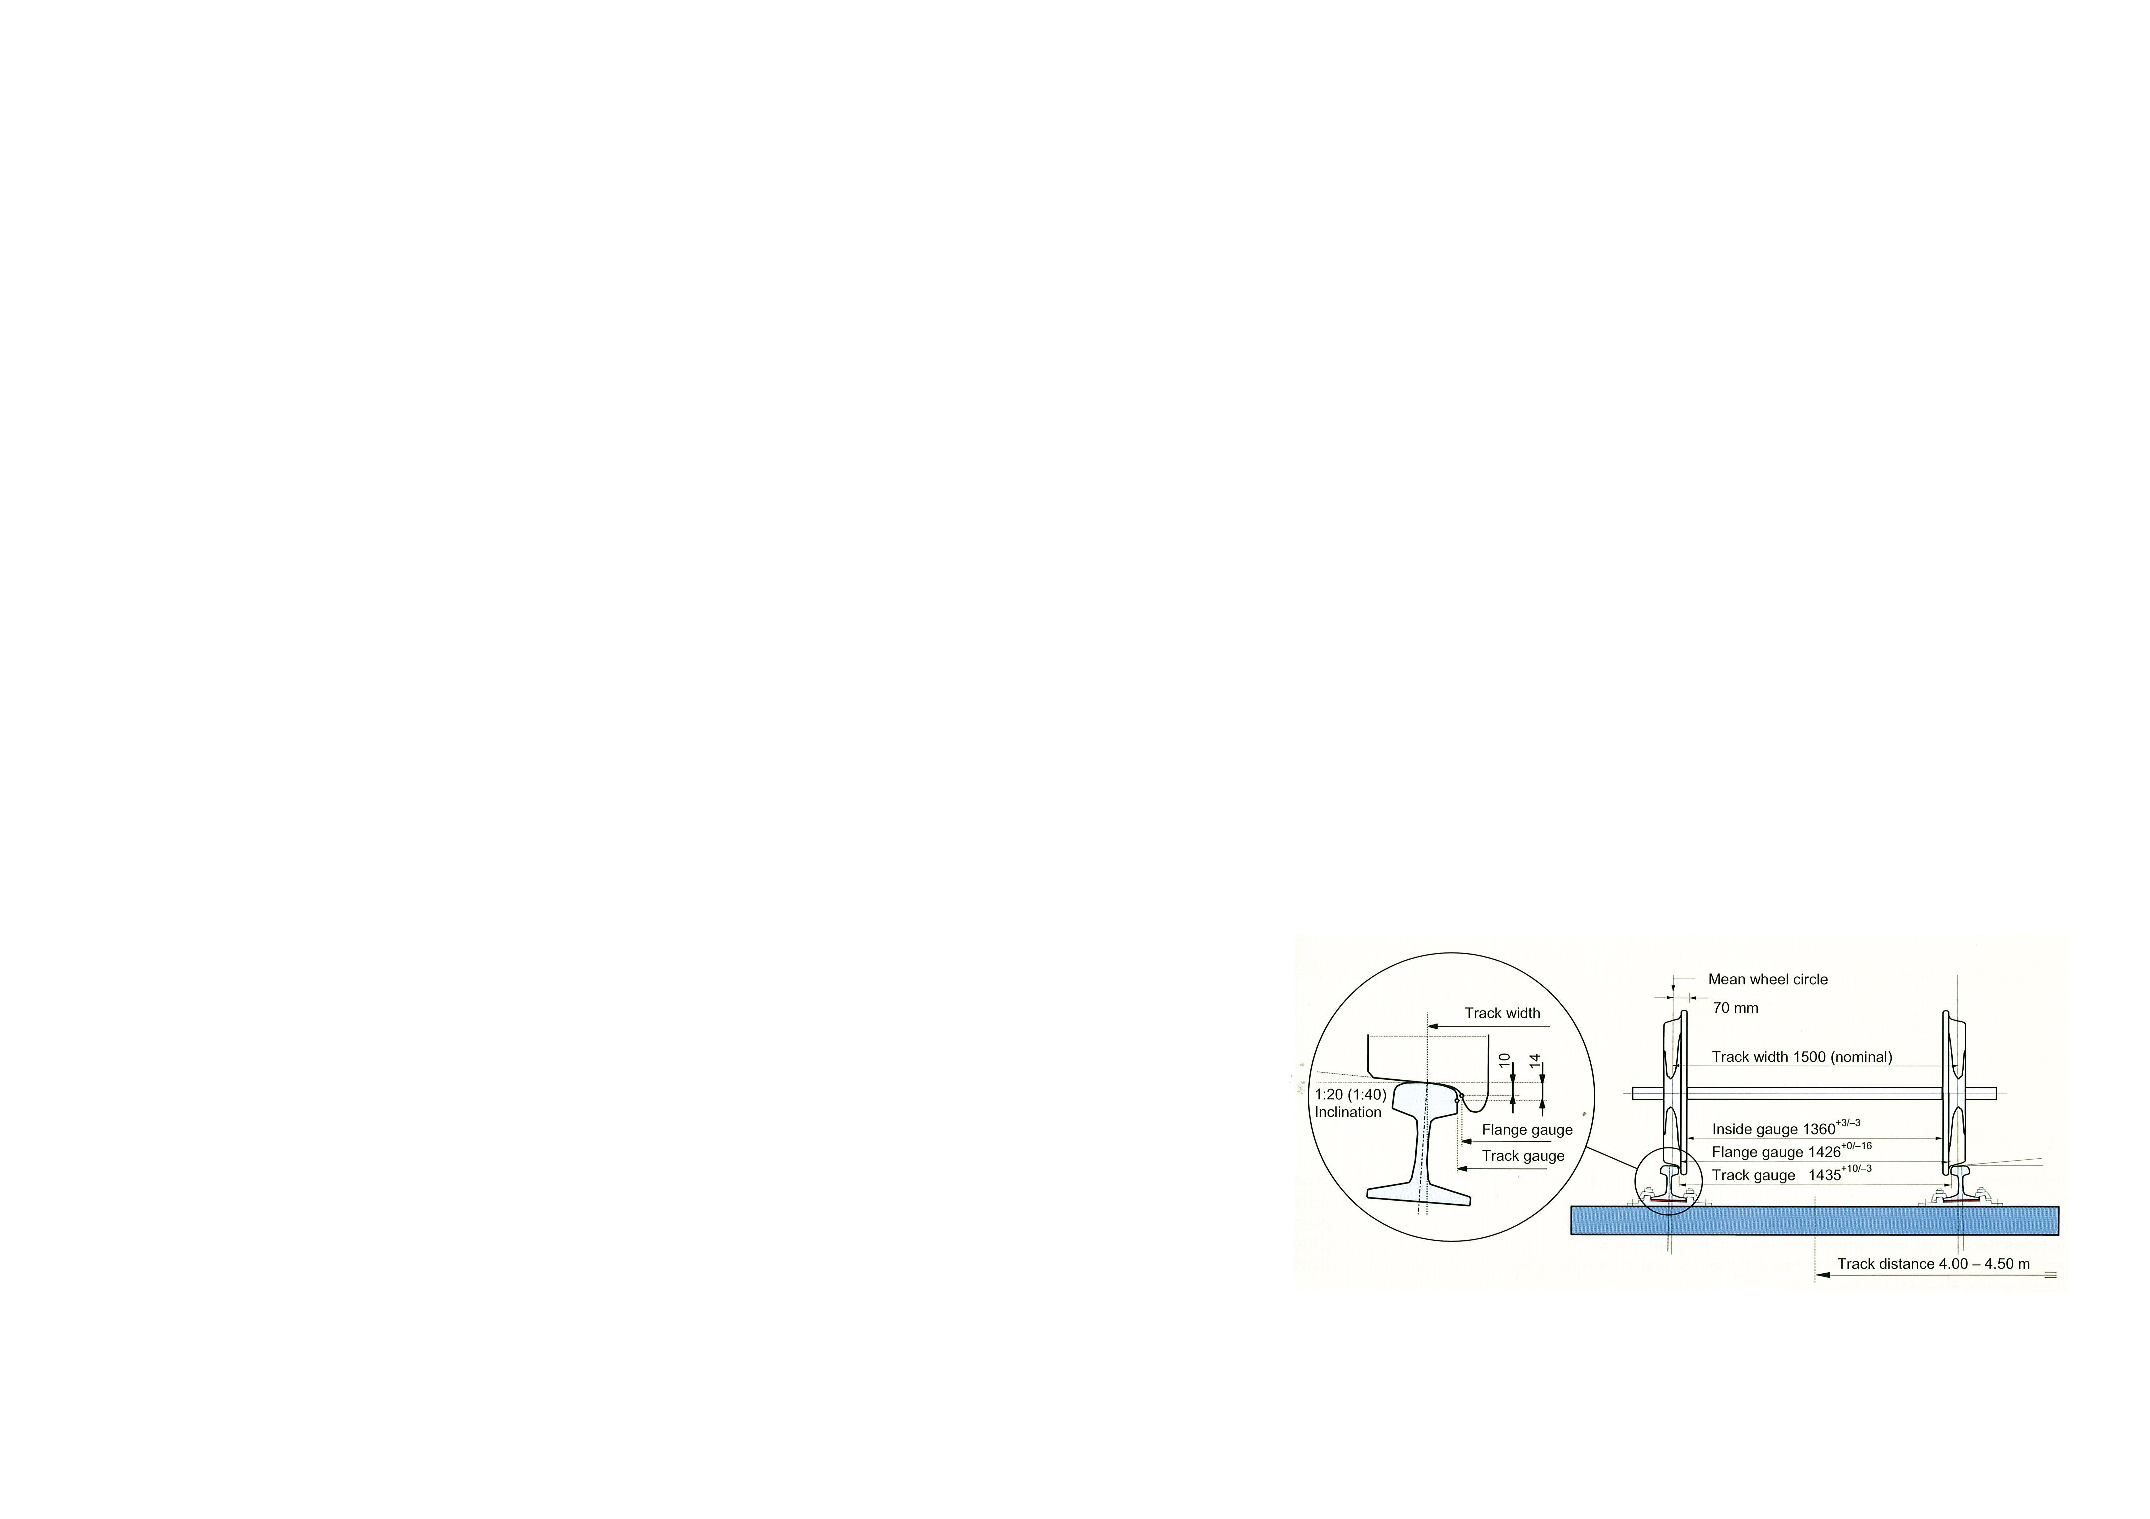
\includegraphics[width=0.5\textwidth]{wheelsettrackdimension.pdf}
\caption{Wheelset and track dimensions. Extracted from \citep[p.17]{esveld2001modern}}
\label{fig:wheelset and track dimensions}
\end{figure}
 
The dimensions of wheelset and track are regulated by International Union of Railways(UIC). Nowadays most of the Dutch rail uses \emph{standard international dimension}. The bridge being designed by Iv-Infra will also apply standard rail dimensions.

The dimension of wheelset and track is explained in Figure.\ref{fig:wheelset and track dimensions}.

Track gauge is defined as a distance between the two rails. On standard track the gauge is $1435^{+10}_{-3}$ mm with with a maximum gradient of $1:3000$. For new track, however, NS apply the following standards\cite{esveld2001modern}:

\begin{enumerate}
\item Mean gauge per 200 m: $1435^{+10}_{-1}$ mm
\item Standard deviation within a 200 m section less than 1 mm
\end{enumerate}

\paragraph{Conicity of wheels and equivalent conicity of wheels}

Conicity of wheels is an important factor influencing the lateral movement of wheelset. Conicity affects the dynamic behavior of wheelsets, therefore affecting the lateral dynamics of the railway vehicles.

The conicity is the inclination of a wheel thread section. Originally conical wheel thread profiles an inclination of 1:20 as shown in Figure.\ref{fig:wheelconicity}. 

\begin{figure}[h!]
	\centering
	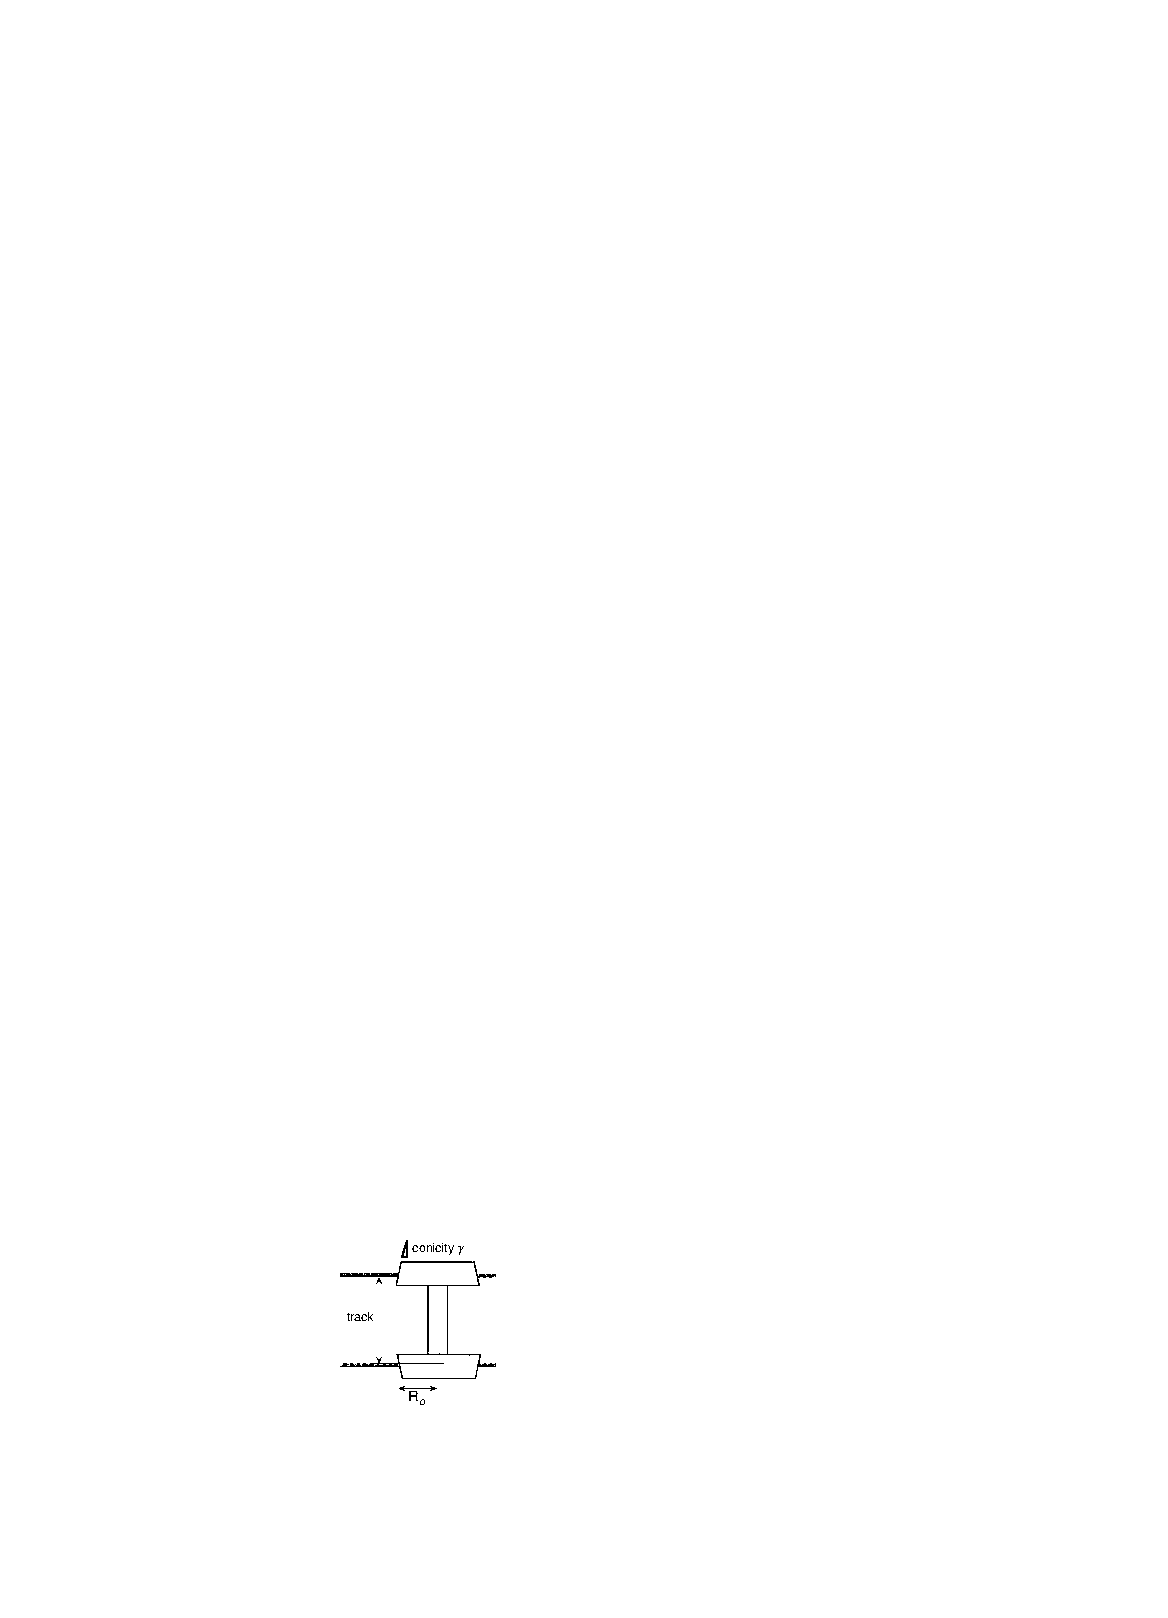
\includegraphics[width=0.3\textwidth]{wheelconicity.pdf}
	\caption{Coning of a wheel thread}
	\label{fig:wheelconicity}
\end{figure}

However, during the manufacturing the tires are given a different shape from a straight conicity. The shape is hollow thus the straight conicity can not effectively describe the geometry of a actual wheel profile. For instance, the S1002 profile defined by UIC is shown in Figure.\ref{fig:s1002}.

\begin{figure}[h!]
	\centering
	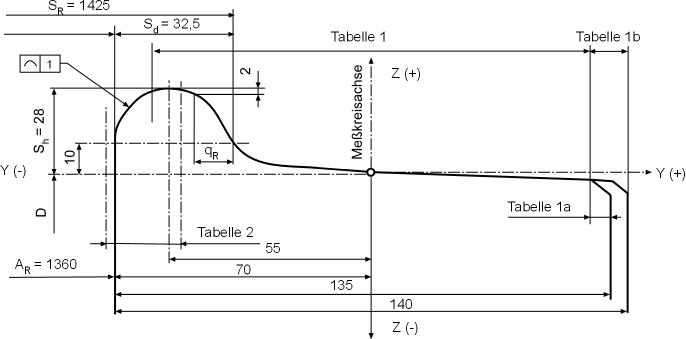
\includegraphics[width=0.5\textwidth]{s1002.jpg}
	\caption{Wheel profile S1002}
	\label{fig:s1002}
\end{figure}

Equivalent conicity is defined to describe the over-all inclination characteristics of a wheel profile. Generally, the equivalent conicity is defined as\cite{esveld2001modern}:

$$ \gamma_e = \frac{\Delta r}{2y} = \frac{r_1 - r_2}{2y}  $$

$r_1 - r_2$ is the instantaneous difference in rolling radius of the wheel treads; generally speaking this is a non-linear function of the lateral displacement y of the wheelset with respect to the central position. 

\paragraph{Worn wheel profiles}

Wheel wears during usage and wheel profiles will change under the effect of wear. Over a period of time wheel profiles stabilize with wear at an equivalent conicity of 0.2 to 0.3\cite{esveld2001modern}. 

\section{Lateral Track Irregularities}
Lateral track irregularities is a source inducing the lateral movement of wheelsets. Track irregularities are minor track deformations that deviate from the original track reference. Well-maintained railway tracks have reduced lateral track irregularities and higher vehicle lateral stability.

The definition is shown in Figure.\ref{fig:lateraldeviationdefine}. See Eurocode\cite{13848} for detailed information about the definition.

\begin{figure}[h]
    \centering
    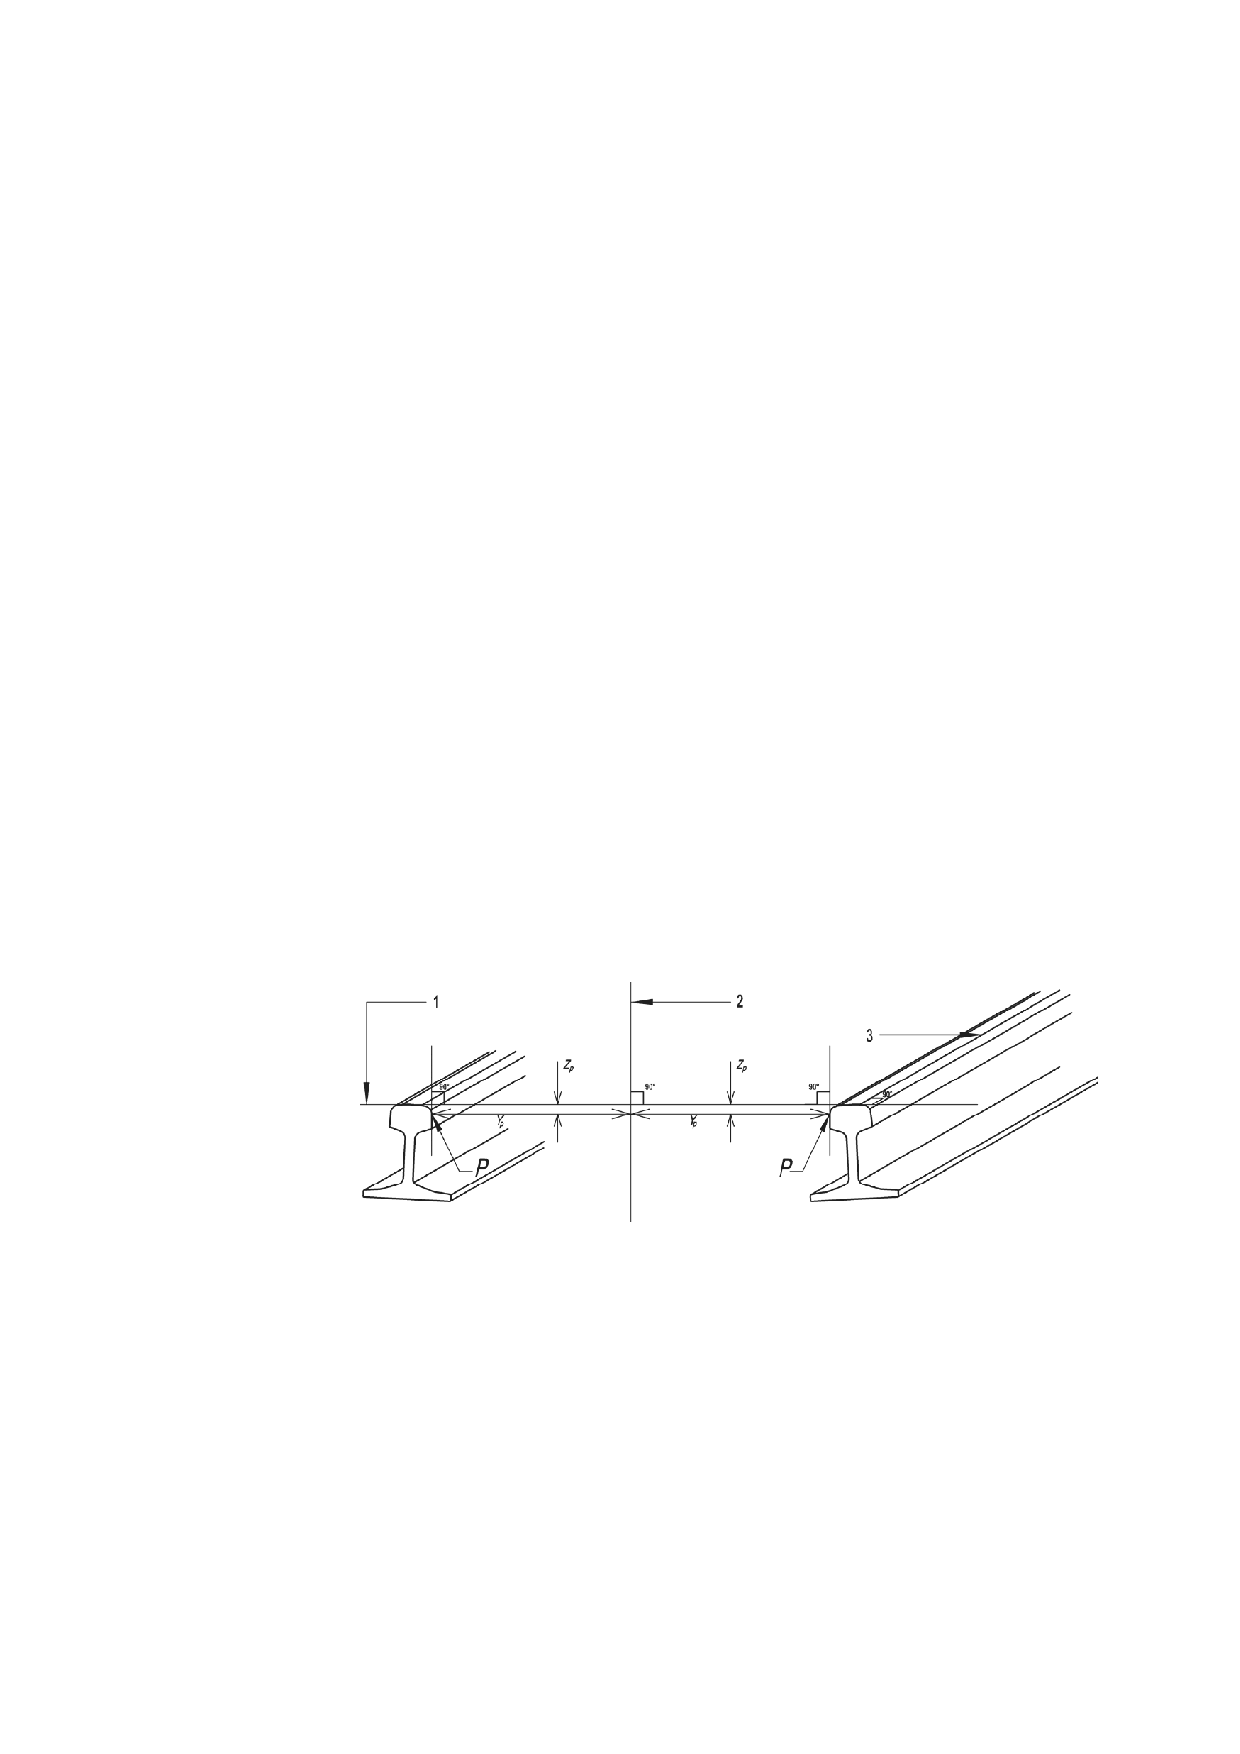
\includegraphics[width=0.8\textwidth]{lateraldeviationdefine}
    \caption{Lateral track irregularity deviation definition\cite{13848}}
    \label{fig:lateraldeviationdefine}
\end{figure}

Table \ref{tab:lateraldeviation}\cite{13848} defines the allowable standard deviation for lateral track irregularities. 

\begin{table}[h]
    \centering
    \caption{Lateral standard deviation\citep[Extracted from][Table B.6]{13848}}
    \begin{tabular}{cc}
        \hline
        Speed(km/h) & Standard deviation(mm) \\
        \hline
        $V\leq 90$ & 1.5 to 1.8 \\
        $80 < V \leq 120$ & 1.2 to 1.5 \\
        $120 < V \leq 160$ & 1.0 to 1.3 \\
        $160 <V \leq 230$ & 0.8 to 1.1 \\
        $230 <V \leq 300$ & 0.7 to 1.0 \\
        \hline
    \end{tabular}
    \label{tab:lateraldeviation}
\end{table}

\section{Lateral movement of wheelsets}
Lateral movement of wheelsets is an essential topic to lateral dynamics of railway bridge because lateral loads on bridge are in direct consequence of lateral movement of wheelsets. 

\paragraph{Contact between wheel and rail}

The movement characteristics of wheels depends on the contact type. There are two types of wheel-rail contact: single-point contact and two-point contact.

In the case of single-point contact, according to Figure.\ref{fig:singlecontact}, wheel load and lateral force act on the same point. This situation occurs when using worn wheel profiles. In the case of two-point contact, shown in Figure.\ref{fig:doublecontract}, the application points do not coincide.

Flanging occurs in the situation of two-point contact. 

\begin{figure}[h!]
\centering
    \begin{subfigure}[b]{0.2\textwidth}
        \centering
        
\includegraphics[width=\textwidth]{singlecontact}
        \caption{Single contact point.  Extracted from \citep[Figure 2.13]{esveld2001modern}}
        \label{fig:singlecontact}
    \end{subfigure}
    \begin{subfigure}[b]{0.5\textwidth}
        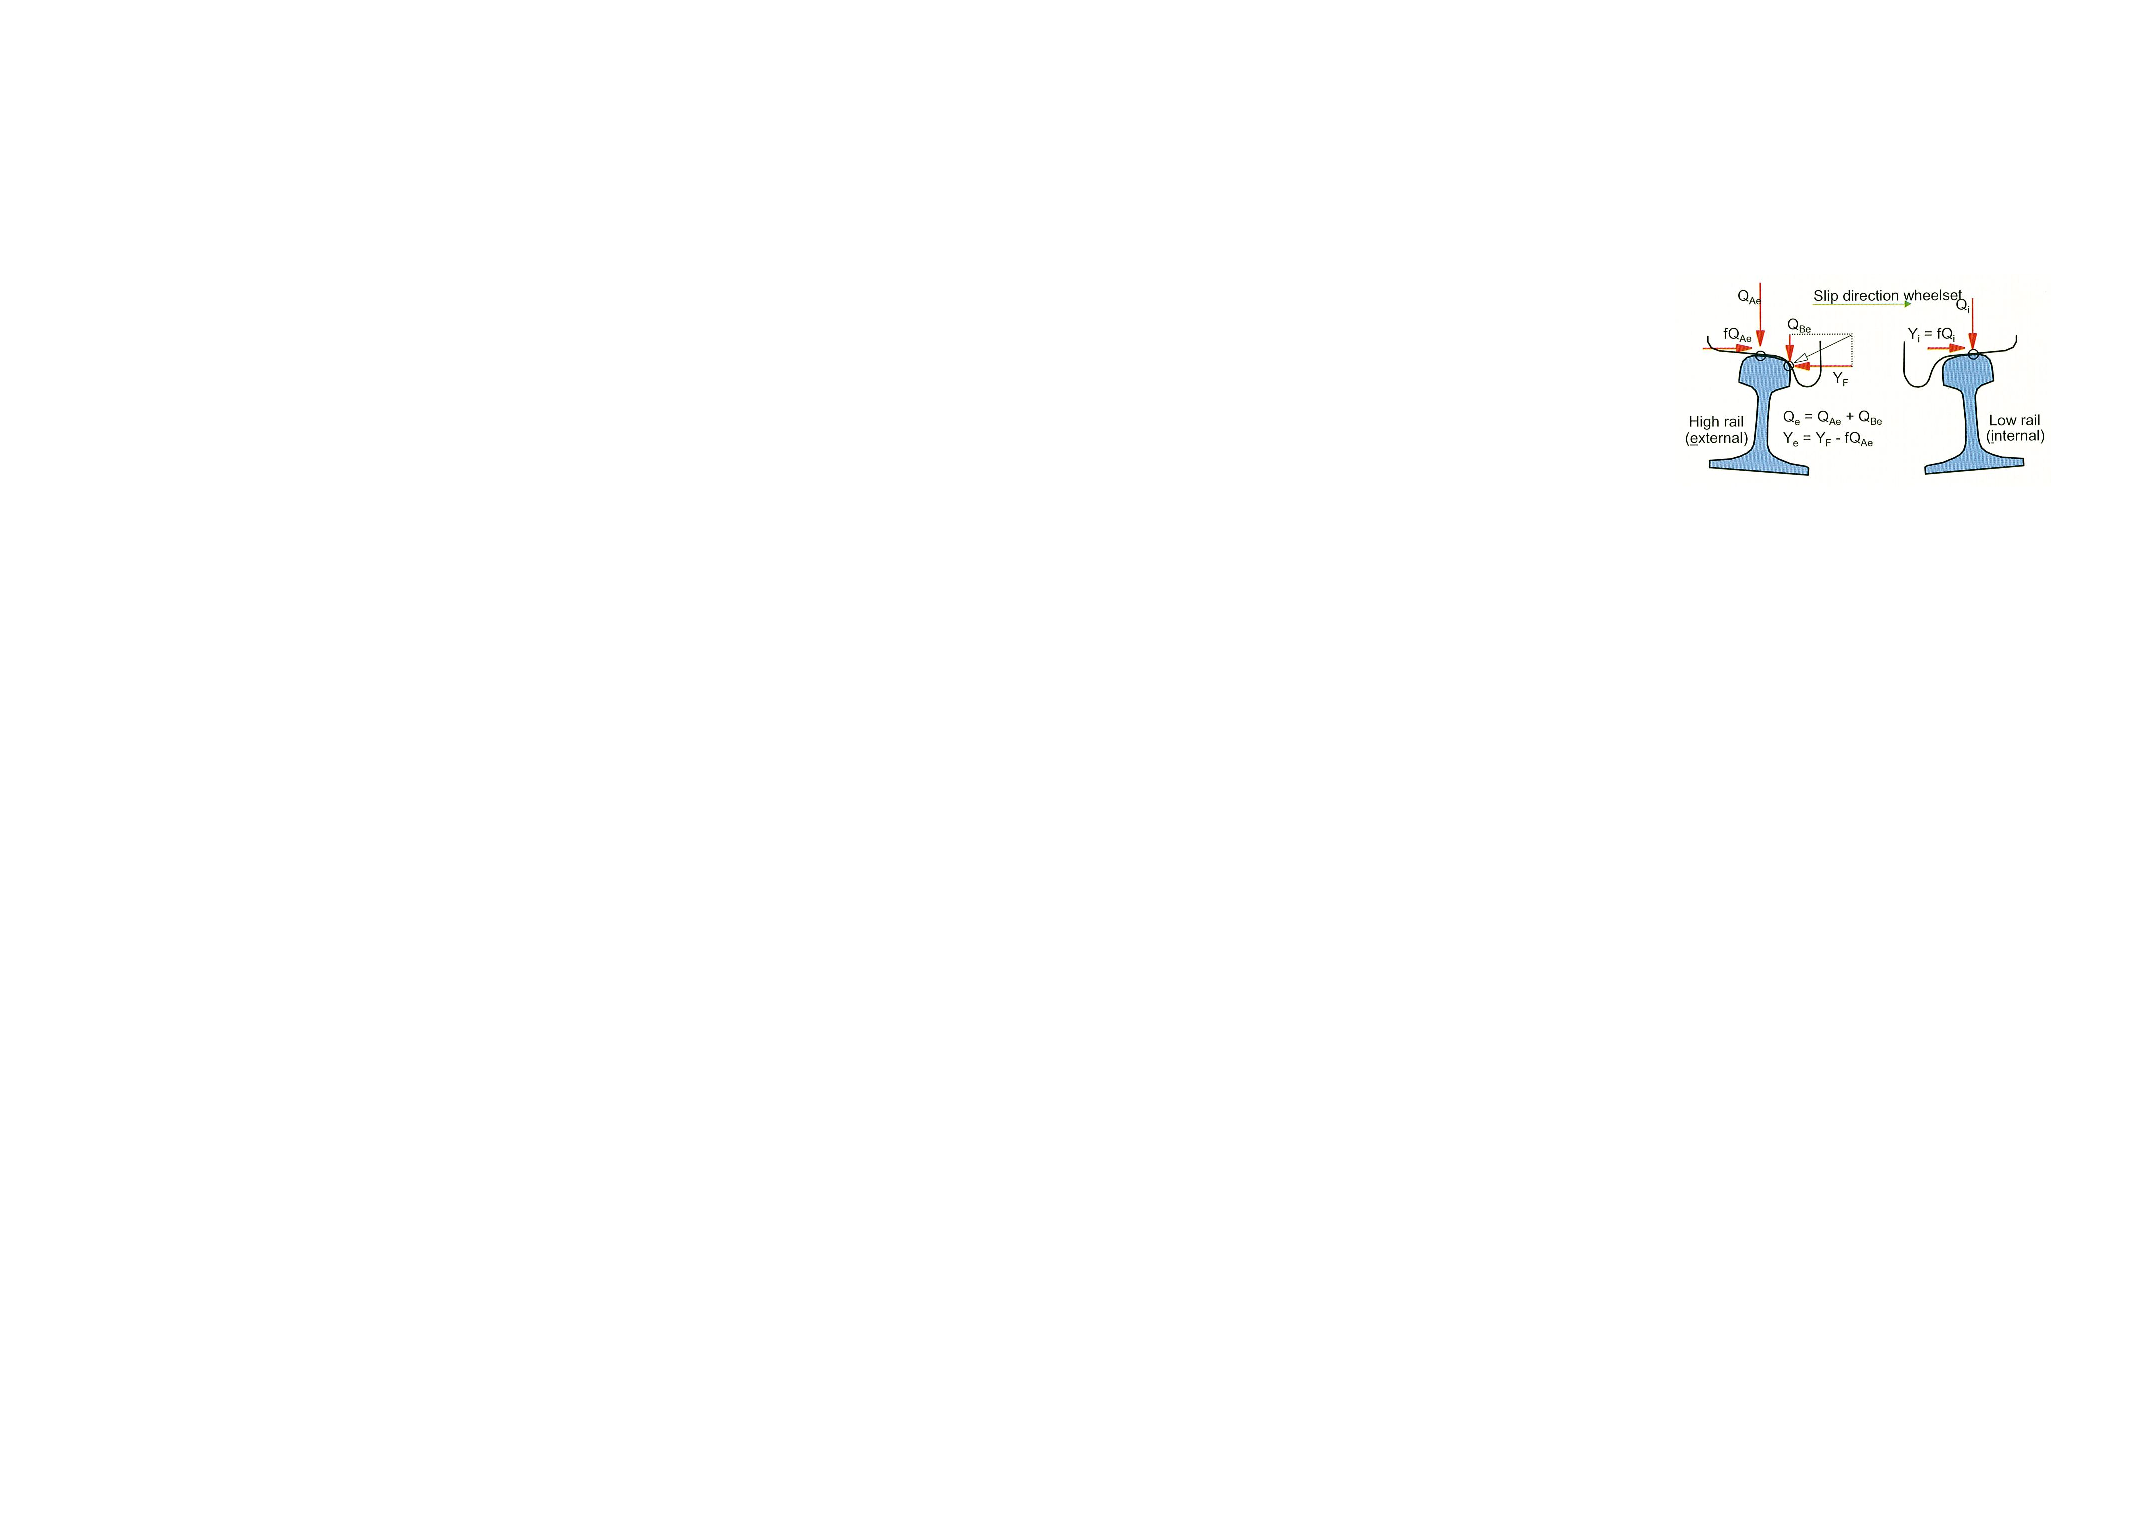
\includegraphics[width=\textwidth]{doublecontact}
        \caption{Double contact points. Forces on rails in case of lateral slip in curves. Extracted from \citep[Figure 2.14]{esveld2001modern}}
        \label{fig:doublecontract}
    \end{subfigure}
    \caption{Single and double contact of wheel-rail interface}
\end{figure}

\paragraph{Klingel movement}

The Klingel movement happens under single-point contact.

Klingel described a periodical movement of the wheelset with conical tire profiles, which is also know as Klingel movement. It was assumed that the wheelset is laterally displaced from central position and the track is ideally straight. This displacement is expected to be counteracted due to different rolling radii of wheels. 

Analysis visualizes the Klingel movement, shown in Figure.\ref{fig:klingelmovement}. The lateral displacement $y$ is a harmonic, undamped function of the distance co-ordinate $x$ as long as the amplitude moves within the wheel flangeway clearance. However, it should be noted that forces play no part in the derivation. Thus Klingel movement is purely a kinematic movement.

\begin{figure}[h]
    \centering
    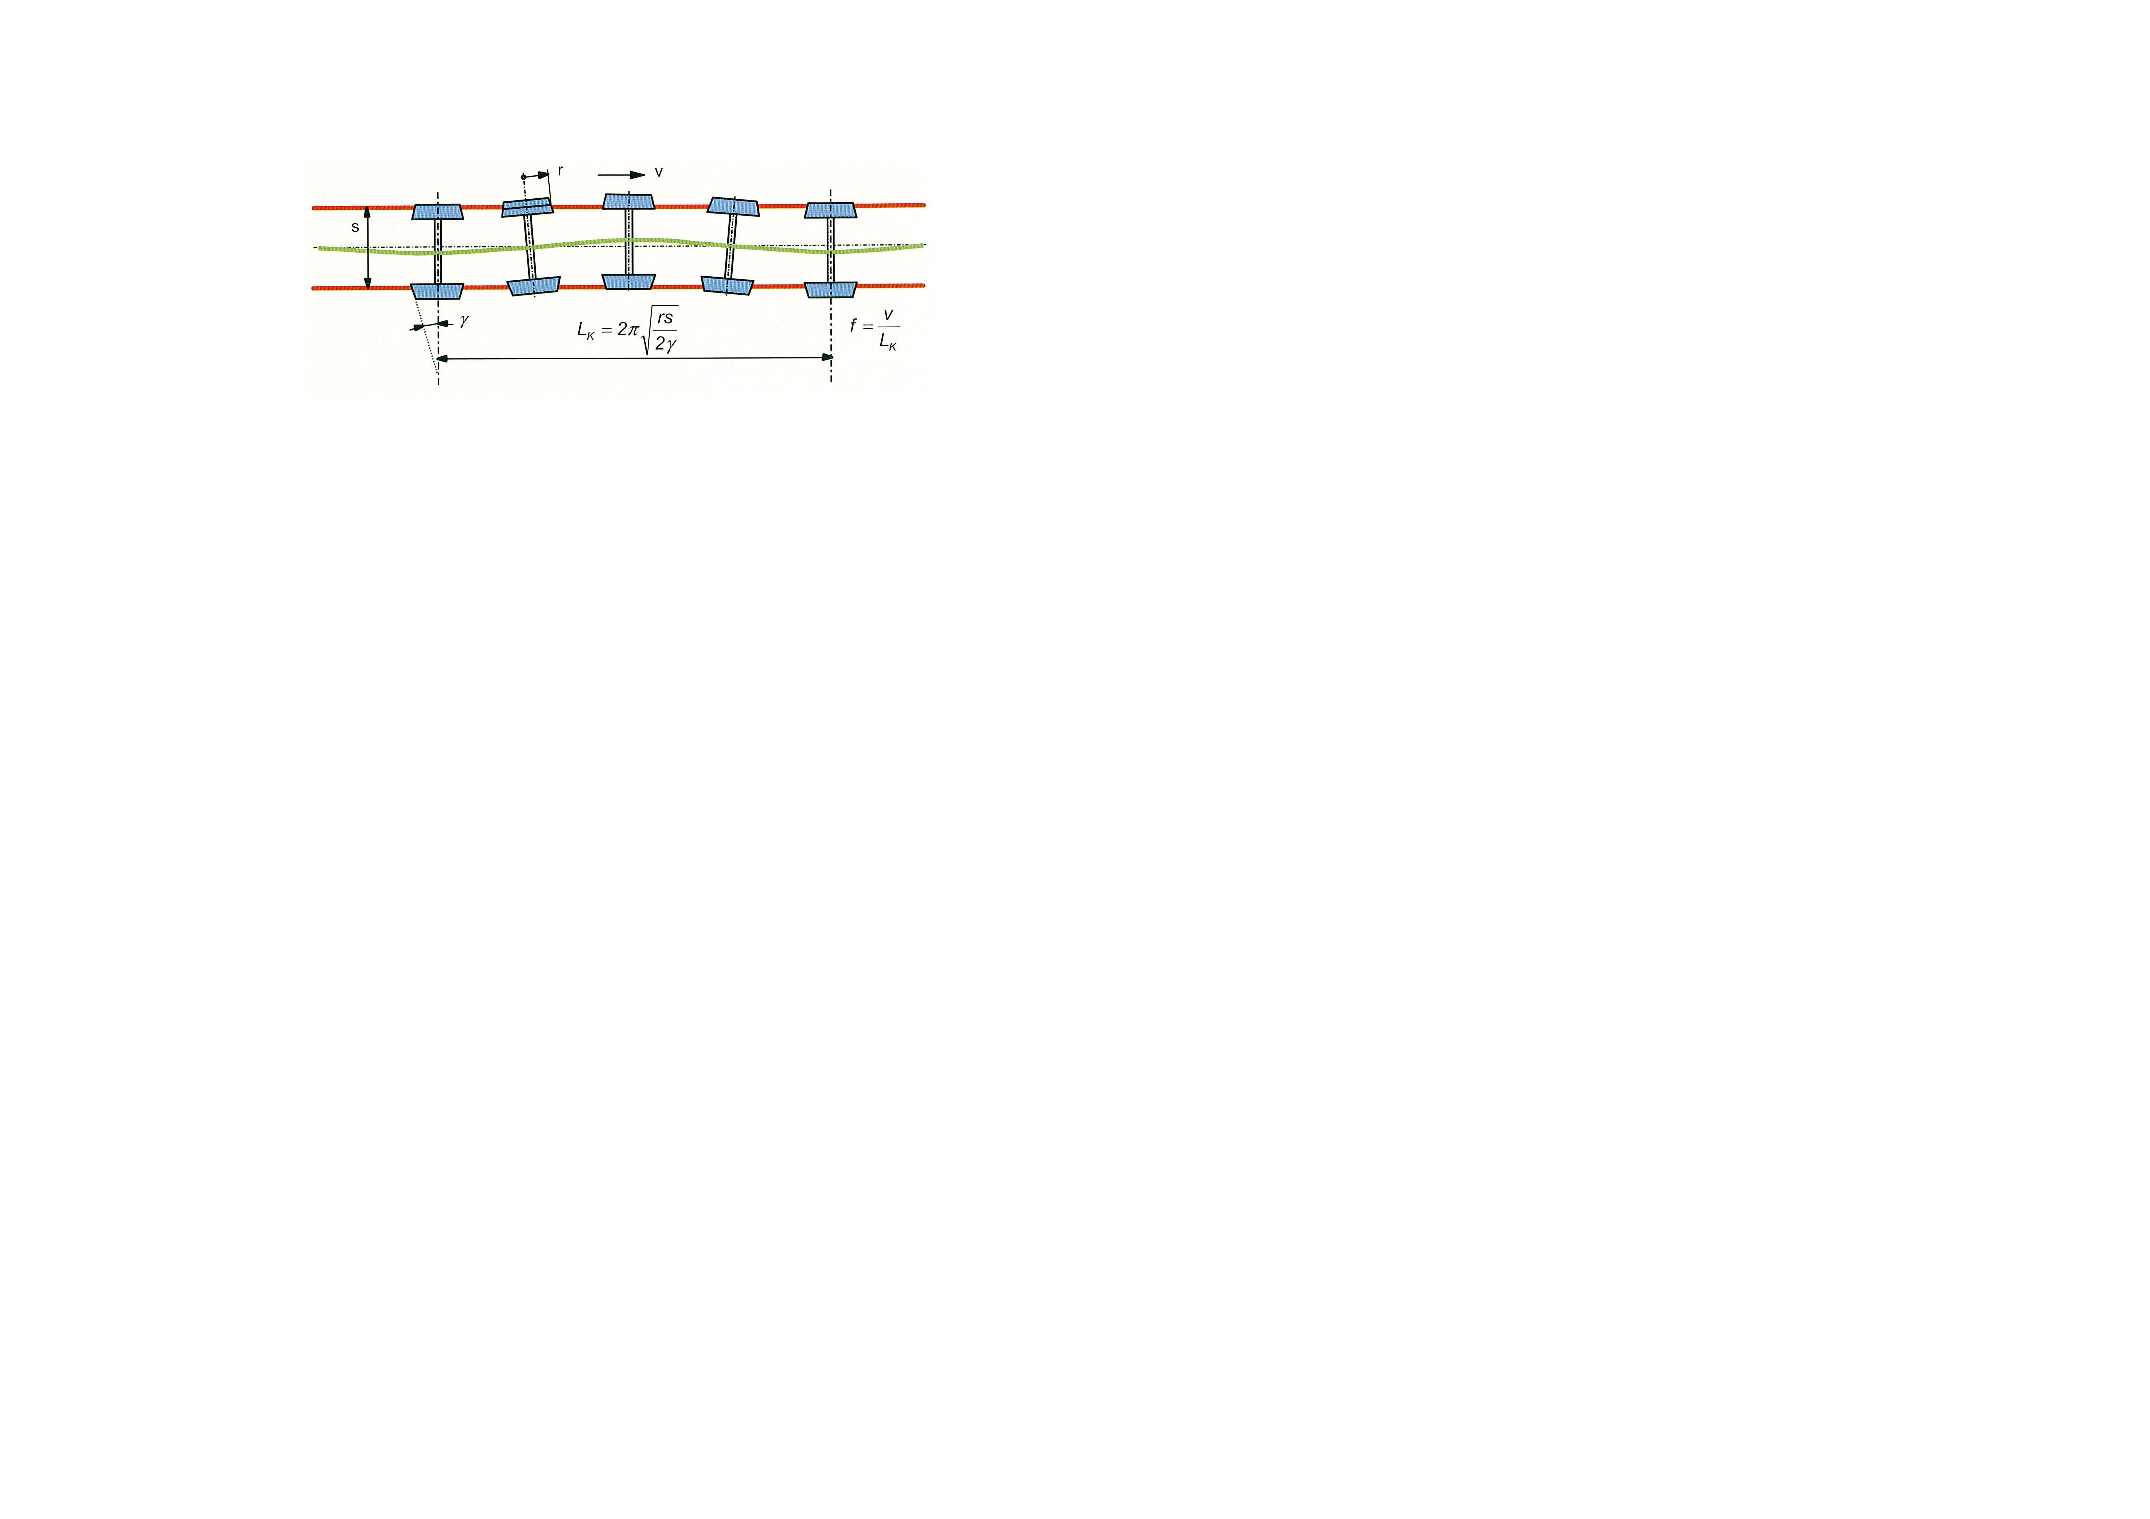
\includegraphics[height = 3cm]{klingelmovement}
    \caption{Klingel movement. Extracted from \citep[Figure 2.3]{esveld2001modern}}
    \label{fig:klingelmovement}
\end{figure}

The expression for wavelength of Klingel movement is shown in Eq.\ref{eq:klingelwavelength}.

\begin{figure}[h]
	\centering
	\begin{equation}
		\label{eq:klingelwavelength}
		L_k = 2\pi\sqrt{\frac{rs}{2\gamma}}
	\end{equation}
	\begin{tabular}{@{}>{$}l<{$}l@{}}
		where: & \\
		L_k & Wavelength of Klingel movement \\
		r & Radius of wheels \\
		s & Gauge distance \\
		\gamma & Conicity of wheels \\
	\end{tabular}
\end{figure}

Introducing the speed, the frequency of Klingel movement is Eq.\ref{eq:klingelfrequency}.

\begin{equation}\label{eq:klingelfrequency}
	f = \frac{V}{L_k} 
\end{equation}

\paragraph{Hunting movement}
The hunting movement happens under two-point contact. Flanging happens in hunting movement.

It should be noted that the Klingel theory is simple and instructive but does not include the effect of coupled axes, mass forces, and adhesion forces. In reality, the amplitude $y_0$ of the Klingel movement is dependent on alignment, dynamic vehicle behavior, and the speed of the rolling stock. 

Generally speaking, $y_0$ due to slip will increase with speed until it is equal to half the flangeway clearance. Flanging then occurs as a result of which the axle will rebound. 

This means that the lateral movement takes on a completely different behavior which is known as hunting. As shown in the drawing in Figure\ref{fig:flangingwheelset} the movement changes from a harmonic to a zig-zag shape. The wavelength becomes shorter and the frequency increases quickly as hunting effect builds up.

\begin{figure}[h]
    \centering
    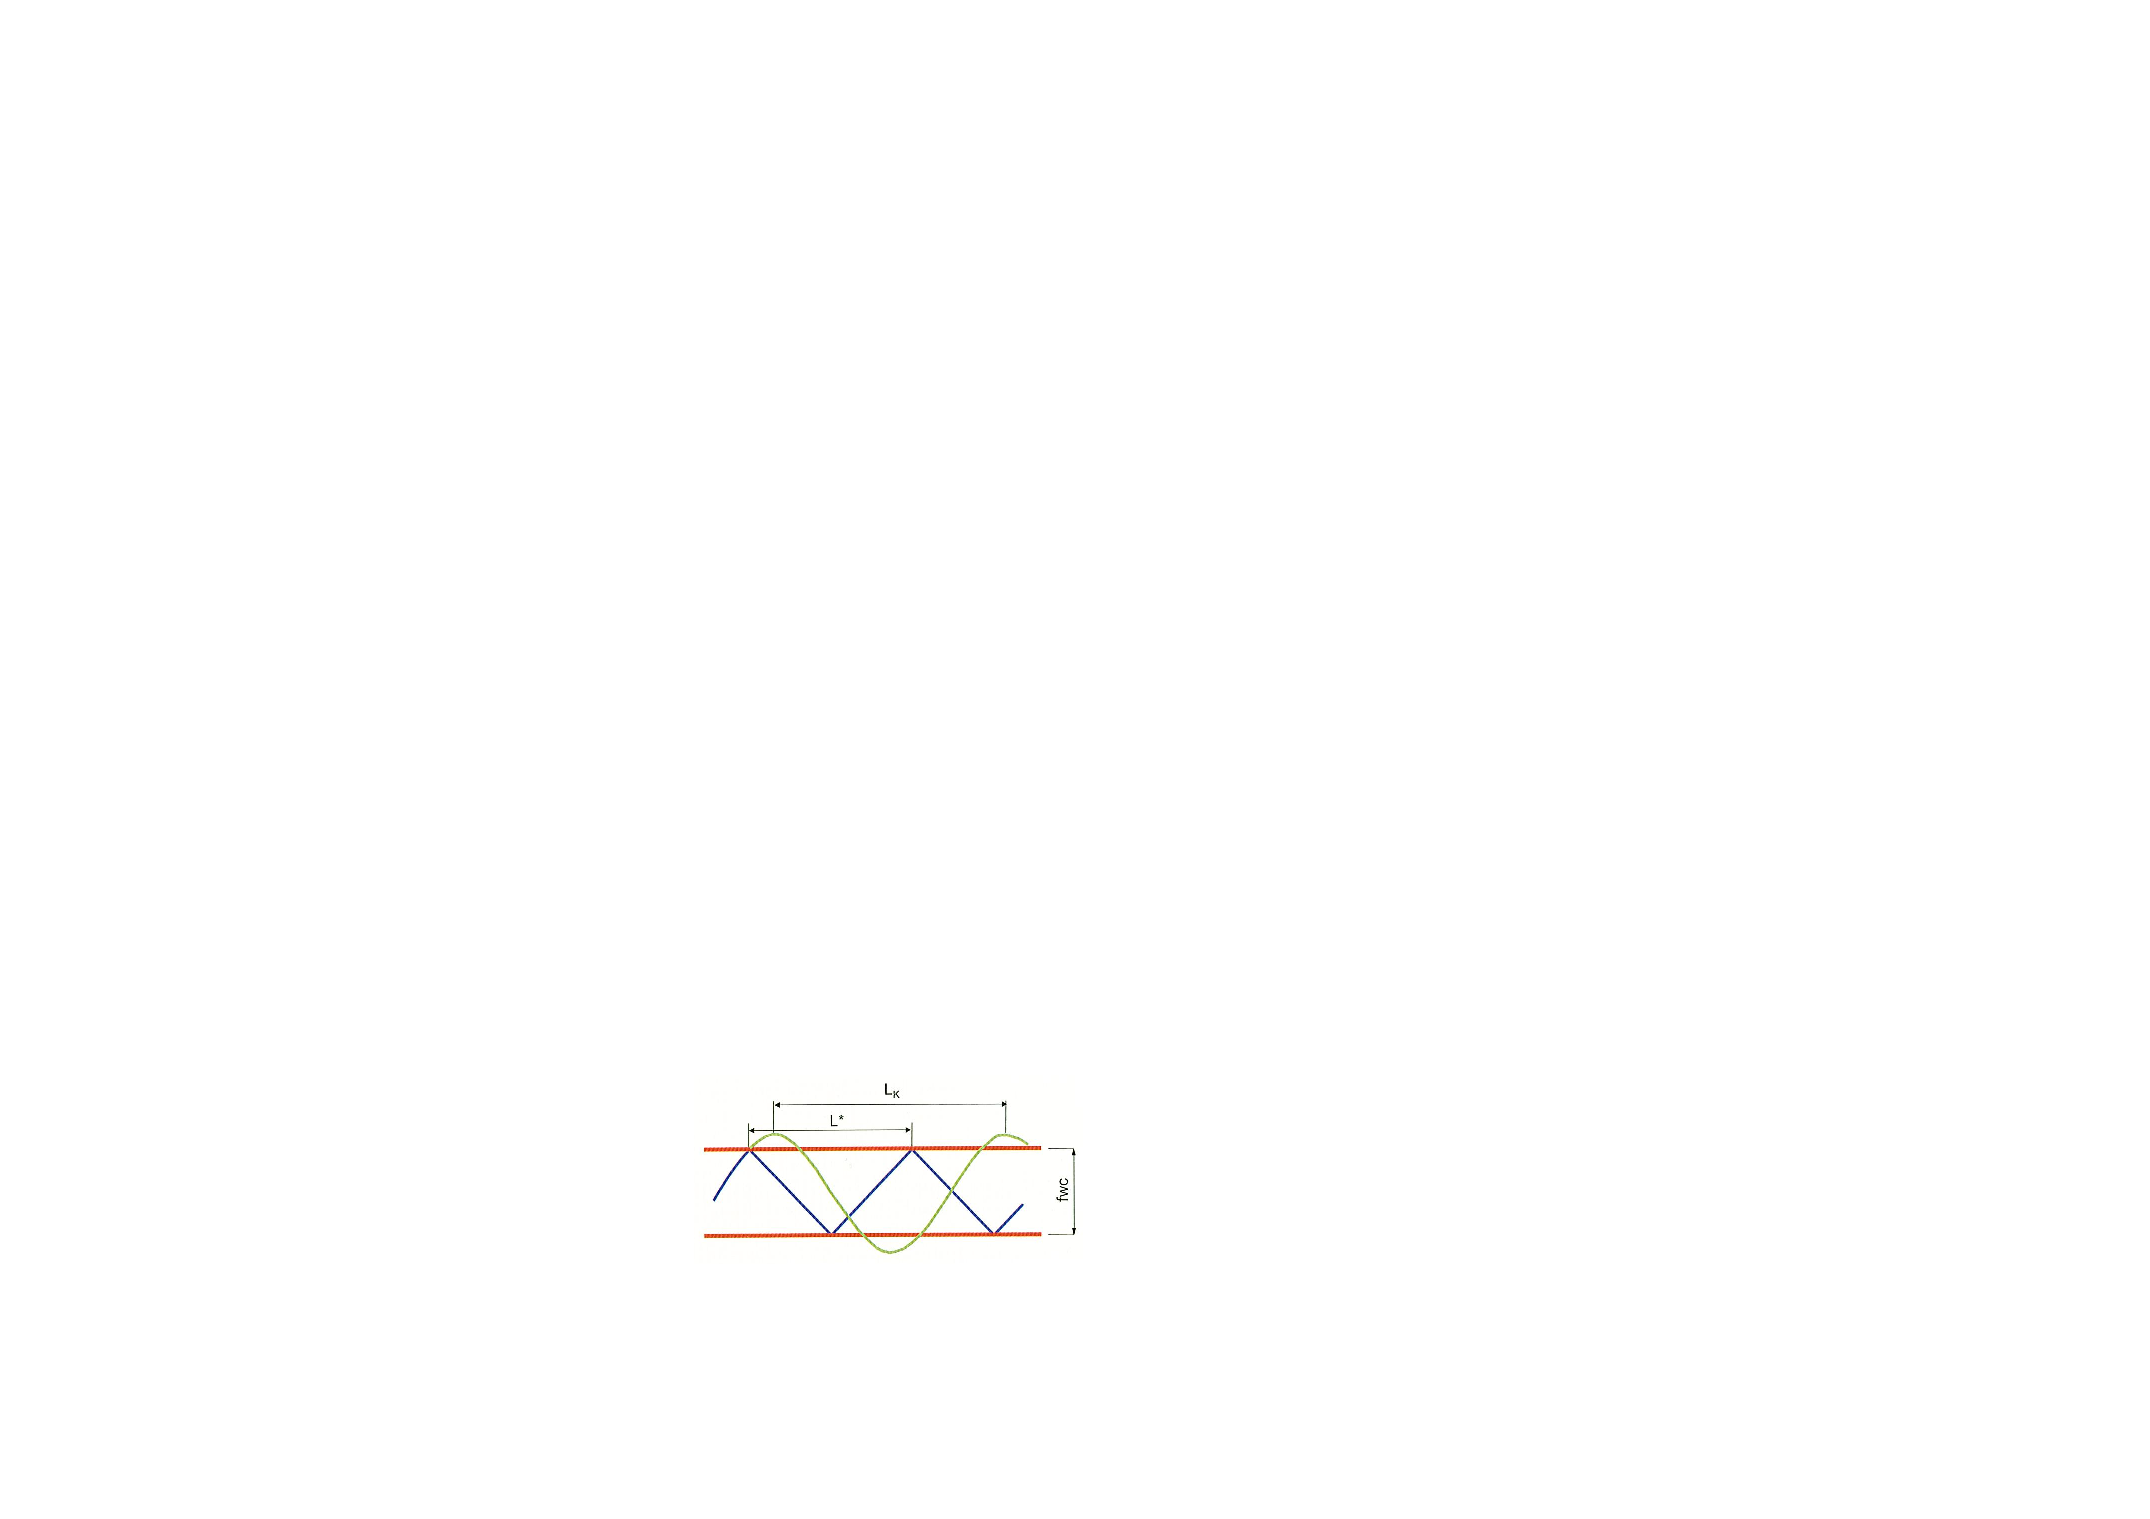
\includegraphics[width=0.5\textwidth]{flangingwheelset}
    \caption{Influence of flanging on lateral wheelset movement. Extracted from \citep[Figure 2.5]{esveld2001modern}}
    \label{fig:flangingwheelset}
\end{figure}

\section{Bridge natural frequency}
The natural frequency of a bridge is an important characteristics of its structural dynamics. 

Research\citep{reberpresentation} shows simplified method can be used to predict the natural frequencies of a bridge. The bridge is modeled as a uniform, simply supported beam. It is validated that the natural frequency of the beam approximately equals to the natural frequency of the bridge.

The beam is simply supported at both ends, and the stiffness of the beam is specified as a deflection at the mid span per unit span length arising from a static point load of 100kN at mid span on the bridge. The length of the beam equals to the span of the bridge. The total mass of the bridge is uniformly distributed over the beam.

The derived natural frequencies of the bridge is shown in Eq.\ref{eq:beamnaturalfrequency}. 

\begin{figure}[h]
	\centering
	\begin{equation}
		\label{eq:beamnaturalfrequency}
		f_r = \frac{r^2 \pi}{2L^2}\sqrt{\frac{EI}{m}}
	\end{equation}
	\begin{tabular}{@{}>{$}l<{$}l@{}}
		where: & \\
		r & Natural mode:1,2,3... \\
		L & Span of the bridge \\
		EI & Equivalent stiffness of the bridge\\
		m & Mass per unit length of the bridge \\
	\end{tabular}
\end{figure}

\section{Lateral vehicle-bridge resonance}
The resonance mechanism between railway vehicle and bridge is a complicated topic. Two types of vehicle-bridge resonance have been validated to be possible by UIC\citep{d181dt329}. They are:

\begin{enumerate}
    \item Resonance caused by axle repeat pattern
    \item Resonance caused by kinematic movement
\end{enumerate}

\paragraph{Resonance caused by axle repeat pattern}
Axle repeat pattern is the periodic pattern of train axles passing on a fixed location. The axle repeat pattern introduces forces to rail track on both vertical and lateral direction. 

The wavelength of the axle repeat pattern is only dependent on the layout of the train. Although the distance between any two axles can form a wavelength, due to the regular arrangement coaches/wagons, there are only a few dominant wavelength. 

Since frequency is speed divided by wavelength, the frequency of the axle repeat patterns vary with train speed. A table of axle repeat pattern lengths, and typical frequencies arising from train speed are given in Figure.\ref{tab:329axlerepeat}

Research\citep[3.4.3]{d181dt329} shows that by running train at different speeds, resonance is possible between train and bridge if the axle passing frequency coincides with the first lateral bridge mode. The resonance effect is more pronounced compared to kinematic movement resonance\citep[Chapter 5, Research Phase II]{d181dt329}.

\paragraph{Resonance caused by kinematic movement}
The lateral kinematic movement of railway vehicles is also wavelength phenomenon. However, the wavelength of lateral kinematic movement is much more complicated than axle repeat pattern. Many factors affect the wavelength of vehicle lateral kinematic movement. These factors include track irregularities, wheel profile, rail profile and other factors that may influence the lateral movement of wheelsets.

The lateral kinematic wavelength of railway vehicles are hard to predict. Research\citep{d181dt329} obtains the lateral kinematic wavelength of the vehicle by numerical modeling a running railway vehicle. 

The frequency of kinematic movement resonance is speed divided by wavelength. By coinciding the lateral kinematic frequency of the vehicle and bridge first lateral natural frequency, the resonance caused by kinematic movement was successfully validated\citep{d181dt329}.

 

%!TEX root = main.tex

\chapter{Analysis of Eurocode criteria}

This chapter aims to analyze the Eurocode criteria that are related to lateral dynamics of railway bridges and discover their background principle. There are two types of criteria: bridge-natural frequency based criterion and vehicle-induced lateral force criterion. 

It has been discovered that UIC research\citep{d181} is the original research that proposed both types of criteria.

\section{Criterion based on bridge natural frequency}

\paragraph{Criterion definition and background}
The bridge natural frequency based criterion is defined in \citep[A24.4.2.4]{EC12} by following statement:

\begin{quote}
	...

	\emph{The first natural frequency of lateral vibration of a span should not be less than $f_{h0}$. The value for $f_{h0}$ may be defined in the National Annex. The recommended value is: $f_{h0}=1.2 Hz$}

	...
\end{quote}

The original proposal can be found in \citep[Proposed criteria]{d181}. The original intension of criterion is explained by following quote text:

\begin{quote}
	\emph{To avoid the occurrence of resonance in the lateral motion of the vehicles due to the lateral motion of the bridge, a limit value lower than the first natural frequency $f_1t$ of the lateral vibration of the span studied should be fixed. The natural frequency for lateral movements is between 0.5 and 0.7 Hz for coaches and between 0.7 and 1 Hz for locomotives. We therefore propose a safety margin $F_{lt} \geq 1.2Hz$}
\end{quote}

\paragraph{Criterion principle} From the original proposal, it can be concluded that this criterion intends to avoid the resonance between the vehicle and the bridge. 

There is no additional explanation about what type of resonance is being avoided. The \emph{natural frequency} in the original text is also unclear. There is no explanation on the natural frequency, either.  

It can be concluded that the original text is referring to the natural frequency of an uncertain vibrating mode of the vehicle. The magnitude of the frequency in original proposal is independent of speed, thus it can be guessed that the frequency refers to the natural frequency of a typical rigid body mode of the vehicle. It may be the lateral swing mode of railway vehicles.

However, the resonance described in the original text does not belong to any resonance type validated in previous research. This is because resonance caused by both axle repeat pattern and kinematic movement happens at frequencies related to vehicle speed. There is no research supports the resonance theory described in this criterion.

As a conclusion, the criterion lacks theoretical support. No evidence proofs the resonance mentioned in the original text can happen.  No background principle can be extracted from this criterion.

\section{Criterion based on vehicle-induced lateral force}
The criterion based on vehicle-induced lateral force is the global criterion governing the validation of structural safety. The criterion itself is generic and unrelated to the topic of lateral dynamics of railway bridge. To be more specific, this section aims to analyze the vehicle-induced lateral force which is a load input for the global criterion.

There are several types of vehicle-induced lateral force mention in Eurocode\citep{EC12} but this thesis only concerns uniform motion and straight railway tracks. Thus one type of force, Nosing force, is selected and analyzed. 

\paragraph{Definition and background of nosing force} 
The nosing force is defined in \citep[6.5.2]{EC12} with following statement:

\begin{quote}
	(1)P The nosing force shall be taken as a concentrated force acting horizontally, at the top of the rails, perpendicular to the centre-line of track. It shall be applied on both straight track and curved track.

	(2)P The characteristic value of the nosing force shall be taken as $Qsk = 100 kN$. It shall not be multiplied by the factor 􏰅$\Phi$ (see 6.4.5) or by the factor $f$ in 6.5.1(4).

	(3) The characteristic value of the nosing force in 6.5.2(2) should be multiplied by the factor 􏰀$\alpha$ in accordance with 6.3.2(3) for values of 􏰀$\alpha$ 􏰁 1.

	(4)P The nosing force shall always be combined with a vertical traffic load.
\end{quote}

The background research\citep{d181dt329} illustrates detailed information about nosing force. The research sets up different scenarios and simulates the scenarios in numerical modeling software. The peak total lateral forces on track are generated from these simulations. After that these peak lateral forces are used to generate the magnitude of the nosing force.

The research obtains peak lateral force by running simulations over a large range of track qualities and wheel conicity from 0.42 mm to 6.2 mm and 0.05 to 0.4 respectively. The track quality range represents a range from best quality high-speed line to poor quality freight track and would therefore be expected to cover the full range of track qualities likely to be found on a railway bridge. The conicity range represents that which can usually be expected to occur for trains running on conventional speed lines.

It has been verified that the peak lateral force on track is greatly affected by track irregularities and wheel conicity. In other words, the poorer the tracks and wheels are maintained, the greater the peak lateral force on track will be. 

\paragraph{Analysis of nosing force}
From the definition of nosing force, it can be seen that nosing force is an imaginary concentrated force which does not represent the real lateral force distribution on track. It aims to represent the total peak lateral force magnitude generated by the whole vehicle. 

For long-span railway bridges, the actual lateral force is axle forces distributed along the the span. Compared to concentrated nosing force, whose magnitude equals to the total sum of magnitude axle forces, the distributed axle force yields lower structural deformation. The nosing force is conservative compared to axle forces in terms of structural mechanics.

However, for nowadays Dutch railways, the wheels and tracks are maintained according to Eurocode regulations so the track irregularities and wheel conicity are well below the most unfavorable scenario simulated in UIC research. This means the peak lateral forces generated by these simulations are too high compared to real peak lateral forces on nowadays Dutch railway tracks. Thus for the same reason, the nosing force whose magnitude is determined using those simulation is too conservative.

\paragraph{Verification on nosing force magnitude}

Nosing force in Eurocode has characteristic value of 100kN, which is lower than the original proposed magnitude in its background research. Additional calculation is carried out to verify if the magnitude is sufficient.

The verification is done by comparing peak displacement caused by 100kN nosing force and peak displacement result of numerical simulation done on the same bridge. The numerical simulation is provide by UIC research\citep{d181dt329}.

\begin{figure}[h!]
    \centering
    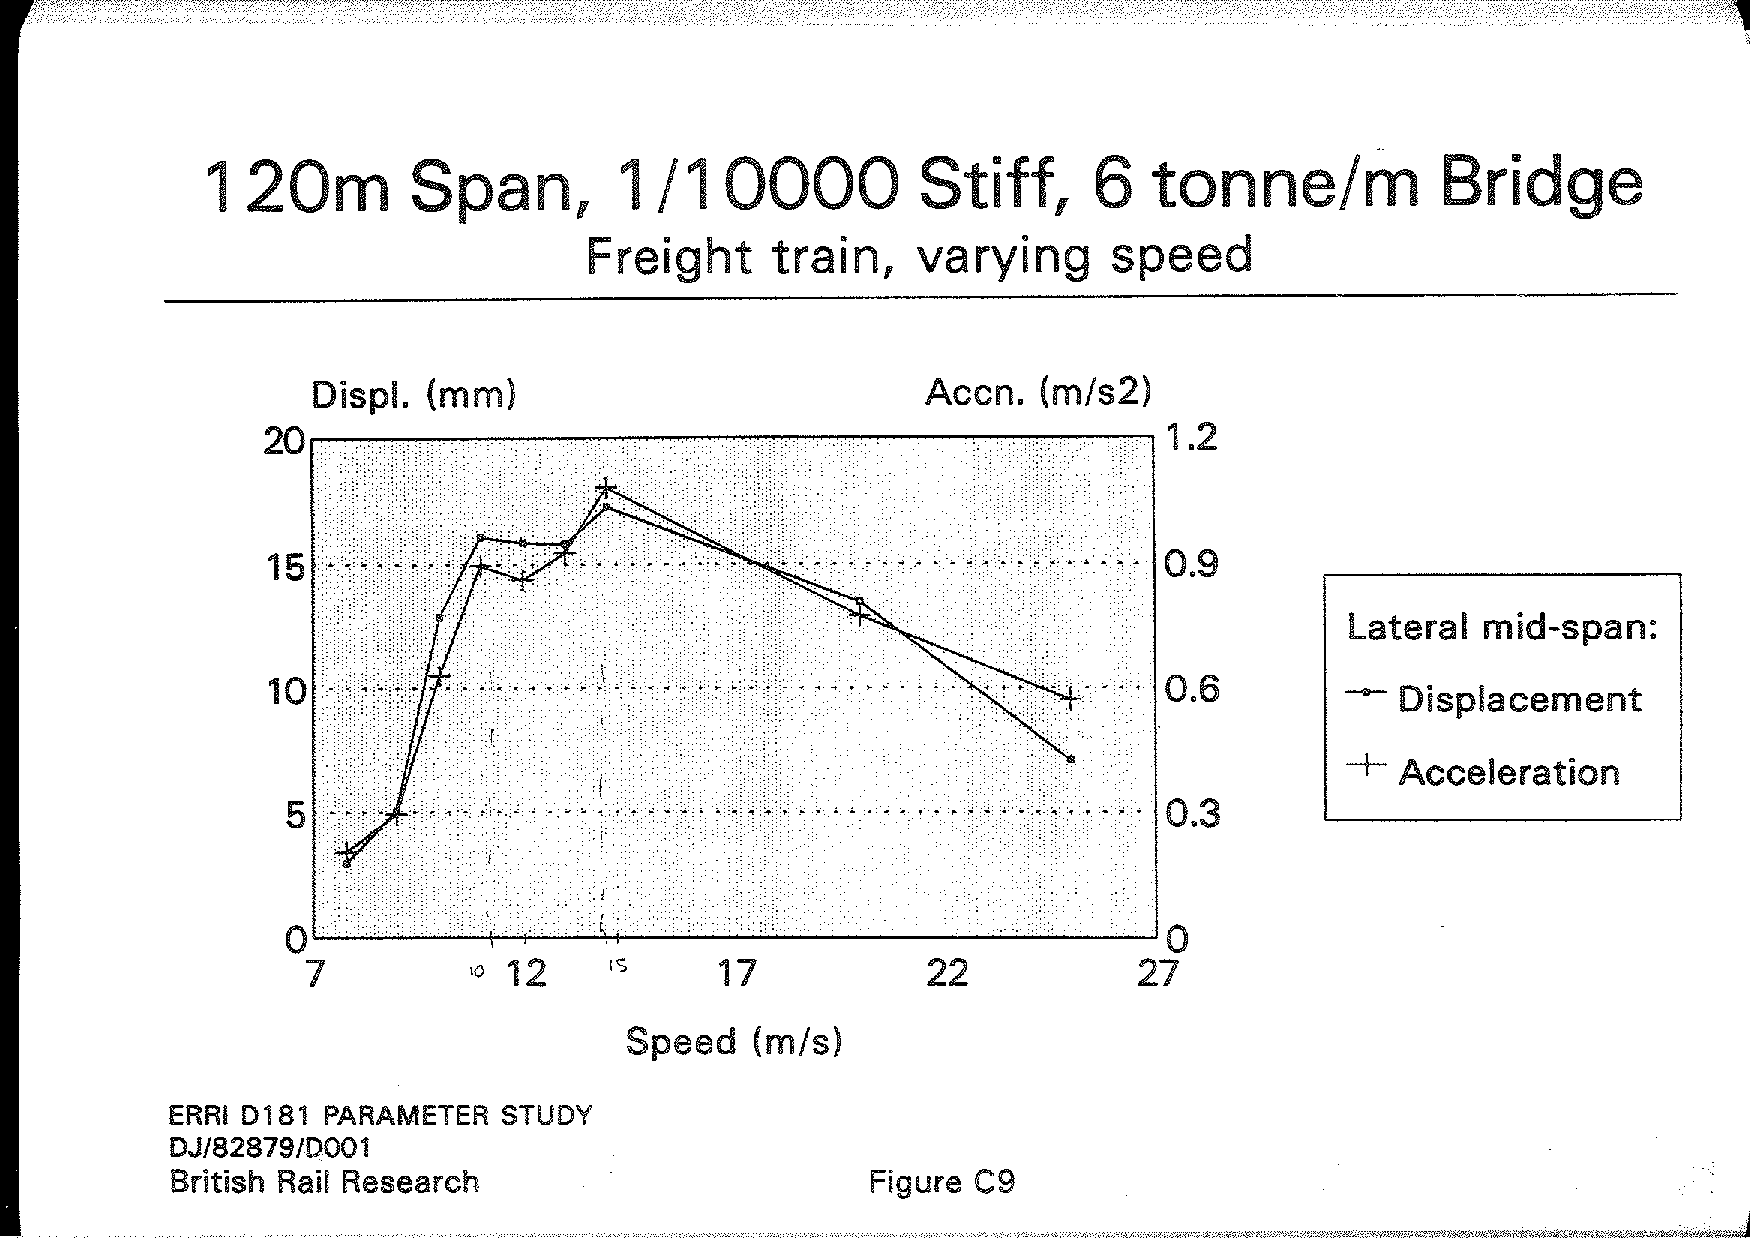
\includegraphics[height = 0.25\textheight]{c9}
    \caption{Figure C9 extracted from \citet{d181dt329} }
    \label{fig:c9}
\end{figure}

Figure.\ref{fig:c9} illustrates a chosen simulation case. The bridge possesses following parameters:

$$
\begin{array}{c}
l = 120m \\ 
Stiff\footnotemark: \sfrac{1}{10000} \\ 
\mu = 6000kg/m\\
\end{array}
$$
\footnotetext{defleciton/span ratio at midspan under 100kN point load at midspan}

Peak result for numerical simulation: 17mm

According to the definition, the characteristic value of the nosing force shall be taken as $Q_{sk} = 100kN$. It shall not be multiplied by the factor $\Phi$ or by the factor $f$. Thus, according to simple support Euler-beam theory, the deflection under 100kN nosing force is:

$$\delta_{nosing} = 120m \cdot \sfrac{1}{10000} = 0.012m = 12mm$$

It can be seen that nosing force does not give conservative result compared to numerical simulations. The reason for the nonconservative result is that this simulation case reproduced vehicle-bridge resonance so the peak displacement is amplified. It can be concluded that nosing force in Eurocode does not take resonance effects into account. It is nonconservative when resonance between vehicle and bridge happens.

\section{Conclusion}
According to the analysis, the Eurocode criterion based on bridge natural frequency lacks theoretical support thus no principle can be extracted from this criterion. The resonance type described in the criterion is not validated by any research and the criterion can not avoid any known resonance type. 

The criterion based on lateral forces is feasible but too conservative in original proposal because nowadays tracks and wheels are well maintained so lateral forces on tracks are much smaller than those generated from UIC simulations. However, nosing force in Eurocode is reduced in magnitude due to unknown reasons and the reduction may result in nonconservative result when resonance happens.

Thus it can be concluded that Eurocode criteria on lateral dynamics of railway bridge lack adequate verification on resonance effects. 

Since the bridge of Iv-Infra can not meet bridge natural frequency based criterion and this criterion is intended to solve resonance issues, the bridge should be verified for its lateral resonance behavior. Since the Eurocode criterion does not make sense, alternative assessment method for lateral railway bridge resonance behavior needs to be applied on the bridge of Iv-Infra.



%!TEX root = main.tex

\chapter{Methods for lateral dynamics assessment}

Several analysing methods for vertical dynamics of railway bridges were briefed in \citet[A6.2]{UIC776-2}. Methods that can be applied also on lateral direction are selected:

\begin{quote}

\emph{...}

\emph{Various programs such as ANSYS, NASTRAN, ABAQUS, SAP, FASTRUDL and so on, can be used to obtain the modal responses of bridge decks. Modeling can be done with beam models using torsional characteristics if the bridge is not a skew bridge and the structure is not a special case (see above). However, spatial modeling is necessary in such cases.}
\emph{...}

\end{quote}


\section{Numerical methods}

When the analysis uses numerical methods to directly integrate the dynamic equation, the loads become the dynamic system in the case of vehicles and their internal behavior impacts the response from the structure.

- the two systems can be considered separate systems,

- the vehicle can be considered a finite element.

This last method takes track profile defects into account and deduces the force of interaction between the structure and the vehicle as well as the internal forces in the dynamic system that is built.

In this method, the equation of the dynamics is solved, with or without prior transformation, by using the conventional algorithms for numerical resolution of second-degree differential equations. These numerical methods calculates the response to regularly spaced time intervals(in general). The selected time pitch determines the accuracy of the results and has a bearing on the length of computer calculations.

Numerical integration methods are all based on the search for balanced solutions of the dynamic equation at regular time intervals.

\paragraph{VAMPIRE}

VAMPIRE is a FEM simulation software developed by DeltaRail. It allows the user to build a dynamic model of any rail vehicle and study the response of the vehicle to real measured track geometry or user specified inputs in the form of track displacements and external force inputs. Rail vehicles can be modeled with simulated instrumentation allowing almost any aspect of behavior to be studied. 

\begin{figure}[h!]
    \centering
    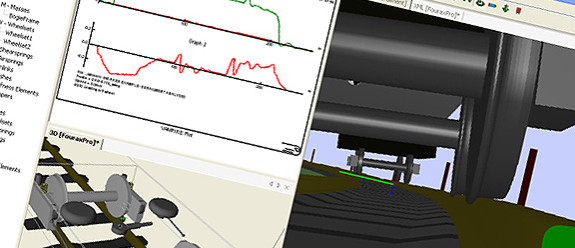
\includegraphics[width=0.8\textwidth]{vampire}
    \caption{A sample project being conducted in VAMPIRE}
    \label{fig:vampire}
\end{figure}

There are also many similar simulation software on the market which puts emphasis on railway vehicle dynamic behavior, but VAMPIRE is specially selected for introduction because it was the software used by UIC committee, whose report series originally proposed 1.2Hz criterion by using the assistance of VAMPIRE. Also, the output results provided by UIC reports is an important foundation for the development of new practical method.

%!TEX root = main.tex

\chapter{Simplified model for assessing lateral railway bridge resonance behavior}
This simplified model aims to simulate the lateral resonance behavior of a railway bridge. 

\section{Assumptions}

It is assumed that the bridge is straight and uniform, simply supported on both ends. One track is installed on the center-line of the bridge. A train is moving uniformly along the track. The train and the bridge are under resonance. Only lateral displacement is taken into account. Deformations of other directions are neglected.

The bridge is modeled as a uniform, simply supported beam. The deflection of the beam represents the lateral deflection of the bridge. The stiffness of the beam is specified as a deflection at the mid span per unit span length arising from a static point load at mid span on the bridge. The length of the beam equals to the span of the bridge. The mass of the beam equals to the mass of the bridge.

A concentrated load presenting the total lateral force induced from the vehicle to the bridge is applied on the beam. The concentrated load is harmonically exciting the beam thus simulating the vehicle-bridge resonance.

The resonance is simulated by setting the magnitude of the concentrated load to oscillate under the same frequency as the first lateral natural frequency of the bridge. The movement of the vehicle is also simulated by setting the load to move at a constant speed, from one end of the beam towards the other end of the beam. 

The force initially locates at one end when time is $0$. Force initial phase is $0$. 

The model diagram is presented Figure.\ref{fig:harmonicloadbeam}.
\begin{figure}[h]
    \centering
    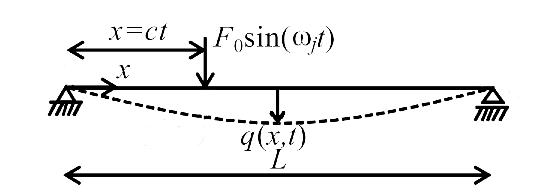
\includegraphics[width=0.5\textwidth]{harmonicloadbeam}
    \caption{Schematic representation of a generic beam crossed by a harmonic load}
    \label{fig:harmonicloadbeam}
\end{figure}

\section{Equation of motion}
The governing equation motion for the model is shown in Eq.\ref{eq:equationofmotion}. 


\begin{figure}[h]
	\centering
	\begin{equation}
		\label{eq:equationofmotion}
		EJ\frac{\partial^4 v(x,t)}{\partial x^4} + \mu\frac{\partial^2 v(x,t)}{\partial t^2} +2\mu\omega_b \frac{\partial v(x,t)}{\partial t} = \delta(x-ct)Q\sin\Omega t
	\end{equation}
	\begin{tabular}{@{}>{$}l<{$}l@{}}
		where: & \\
		EJ & Lateral stiffness of the beam \\
		v & Lateral displacement of the beam \\
		x & Horizontal axis label\\
		\mu & Mass per unit length of the beam \\
		\omega_b & Circular frequency of damping \\
		c & Speed of moving load \\
		Q & Amplitude of load \\
		\Omega & Circular frequency of load. $\Omega$ equals to first lateral \\
		& natural frequency of the bridge \\
		\delta & Delft function \\
	\end{tabular}
\end{figure}


\section{The explicit solution}
The explicit solution of the motion equation is derived by Fryba\citep{fryba1999vibration}. Derived equation for mid-span lateral displacement is Eq.\ref{eq:v(x,t)simpleharmonic}. \emph{This equation will be referred as 'the explicit solution' in following paragraphs.}

\begin{figure}[h]
	\centering
	\begin{equation}
		\label{eq:v(x,t)simpleharmonic}
		v(\sfrac{l}{2},t) = \frac{l^3Q\omega_{(1)}}{\pi^4 EJ}\frac{\cos \omega_{(1)}t}{\omega^2+\omega_b^2}[\omega(\cos\omega t - e^{-\omega_b t})-\omega_b\sin\omega t]
	\end{equation}
	\begin{tabular}{@{}>{$}l<{$}l@{}}
		where: & \\
		l & span of the beam($m$) \\ 
		\zeta & damping ratio \\
		\omega_1 & first natural circular frequency of the beam \\
		& $=\frac{\pi^2}{l^2}\sqrt{\frac{EJ}{\mu}}$\\
		\omega & $= \sfrac{\pi c}{l}$ \\
		\omega_b & = $\frac{1}{2}\zeta\omega_1$ \\ 
	\end{tabular}
\end{figure}

\paragraph{Damping in the expression}
This paragraph aims to derive the correct expression for the damping component in the expression for Eq.\ref{eq:v(x,t)simpleharmonic}.

Eq.\ref{eq:equationofmotion} uses a form of damping expression $\omega_b$, which can be converted from normal damping coefficient. Equation of motion using damping coefficient is shown in Eq.\ref{eq:equationofmotiondampingcoefficient}:

\begin{equation}\label{eq:equationofmotiondampingcoefficient}
    EJ\frac{\partial^4 v(x,t)}{\partial x^4} + \mu\frac{\partial^2 v(x,t)}{\partial t^2} +\chi \frac{\partial v(x,t)}{\partial t} = \delta(x-ct)Q\sin\Omega t 
\end{equation}

where $\chi$ stands for damping coefficient. By comparing \ref{eq:equationofmotiondampingcoefficient} and \ref{eq:equationofmotion}:

\begin{equation}
    \omega_b = \frac{\chi}{2\mu}
\end{equation}

where:

$\omega_b$: circular frequency of damping

$\chi$: damping coefficient

$\mu$: mass per unit length of the bridge

also, in \citep[Page.704]{abu2000vibration} it is mentioned that:

\begin{quote}
    The external and internal damping of the beam are assumed to be proportional to the mass and stiffness of the beam respectively,i.e., $r_a = \gamma_1 \mu$.., where $\gamma_1$ and $\gamma_2$ are proportionality constants.
\end{quote}

thus:


\begin{equation}
    \omega_b = \frac{\gamma_1}{2}
\end{equation}

and it is mentioned in \citep[Eq.8]{abu2000vibration} that:

$$\zeta = \frac{\gamma_1}{\omega_1}$$

so:

$$\gamma_1 = \zeta\omega_1$$

so:

$$\omega_b = \frac{1}{2}\zeta\omega_1 = \frac{1}{2}\frac{\zeta\pi^2}{l^2}\sqrt{\frac{EJ}{\mu}}$$


\section{Mathematical validation of derived expressions}

Since circular frequency of damping $\omega_b$ is not clearly defined by Fryba, it is necessary to verify the correctness of both explicit solution and deduced $\omega_b$ expression.

The verification is done by comparing the result of Eq.\ref{eq:v(x,t)simpleharmonic} with the result of a explicit solution in a different form obtained by another deducing method.  

The result in \citet{abu2000vibration} is selected to be the benchmark for verification. This report is researching vibration of beams with general boundary conditions due to a moving harmonic load. The differential equation is illustrated as follows:

\begin{equation}\label{eq:hilal}
    EIv''''+\mu \ddot{v} + r_a \dot{v}+r_i \dot{v}''' = p(x,t)
\end{equation}

The difference between Eq.\ref{eq:hilal} and Eq.\ref{eq:v(x,t)simpleharmonic} is that it offers broader boundary conditions such as changing speed of the load and various kinds of supports. As a result of more general equation, the deduction steps are much more complicated. However, two solutions should yield same results under same boundary conditions that:

\begin{enumerate}
    \item Load moving at constant speed,
    \item Frequency of load equals frequency of the beam,
    \item Internal damping is 0,
    \item Simple hinge support at both ends of the beam.
\end{enumerate}

One plot from the parametric study of \citet{abu2000vibration} meets the above requirement and is selected and illustrated in Figure. Parameters used in this plot is $\alpha = 0.25$, $\zeta = 0.05$, $\beta  = 1$

\begin{figure}[h!]
    \centering
    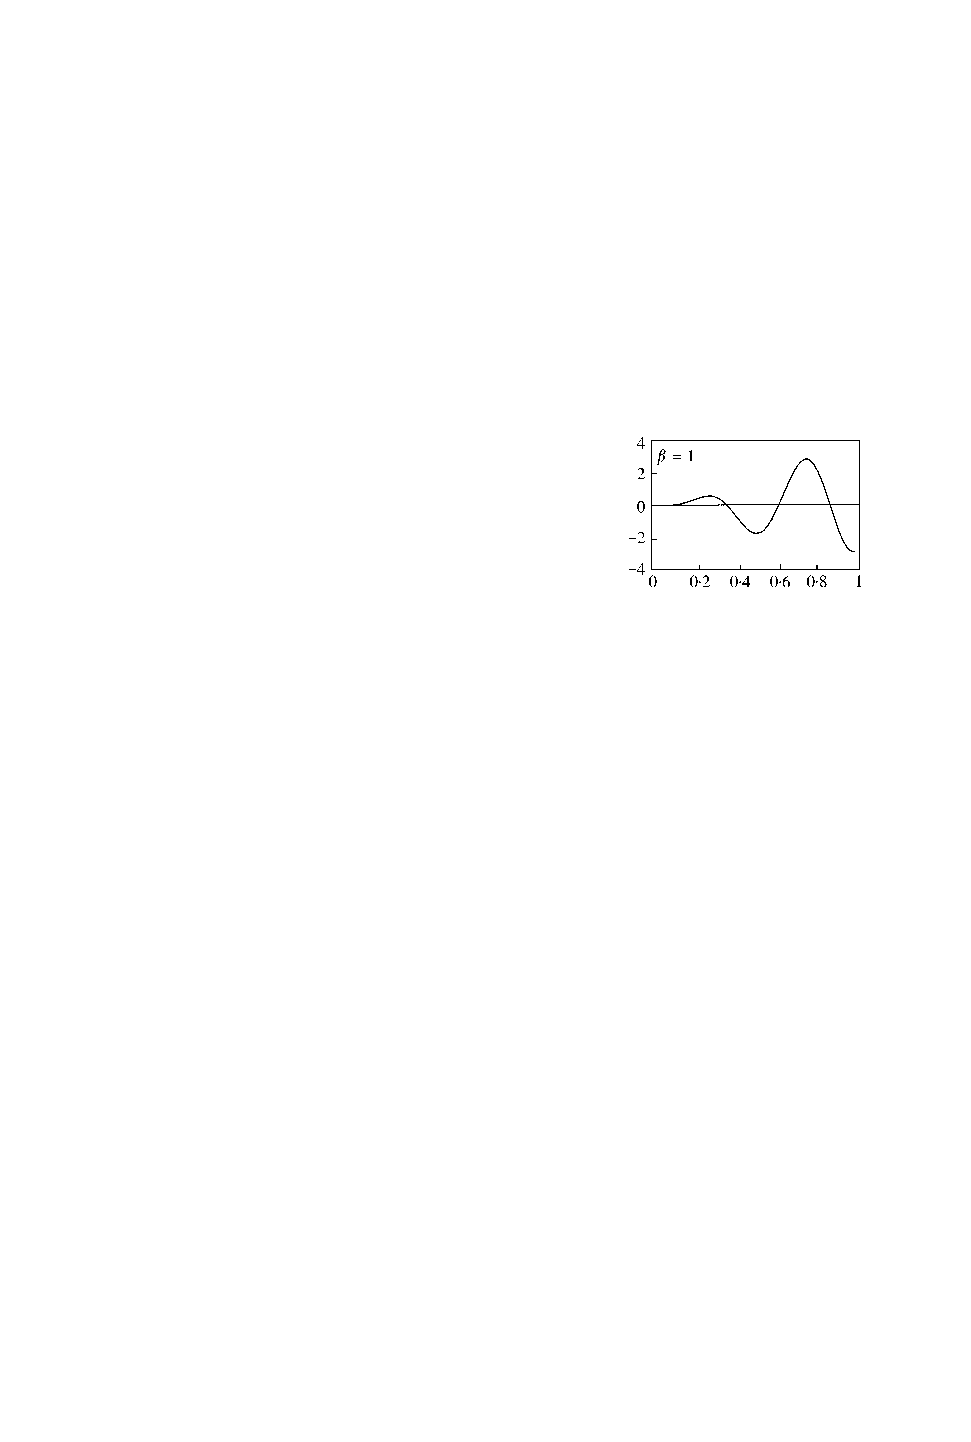
\includegraphics[height = 0.25\textheight]{hilalplot}
    \caption{Reference plot extracted from \citet{abu2000vibration}. Condition: $\alpha = 0.25$, $\zeta = 0.05$, $\beta  = 1$. Y axis for dynamic amplification factor.}
    \label{fig:hilalplot}
\end{figure}

Next step is to translate parameters used in above plot to usable parameters in Eq.\ref{eq:v(x,t)simpleharmonic}.


$$c_{cr} = \frac{\omega_1 L}{\pi} = \frac{\pi}{l}\sqrt{\frac{EJ}{\mu}}$$

$$c = \alpha c_{cr} = \frac{\alpha\pi}{l}\sqrt{\frac{EJ}{\mu}}$$

$EJ$,$\mu$,$l$ needs to be selected to yield value for $c$, thus following values are randomly selected:

$$
\begin{array}{c}
	EJ = 2.43e10 Nm^2 \\
	l = 54m \\
	\mu = 6000 kg/m \\ 
	c_{cr} = 117.05 m/s \\
	c = 29.26 m/s  \\
\end{array}
$$

A Matlab script is written to automate numerical calculating procedure. The script is presented in Appendix.\ref{sec:matlabscripts}. By typing 

\texttt{>>fog(2.43e10,54,6000,29.26,0.05)}

into the console. Figure.\ref{fig:EJ24300000000L54mu6000c29daf.tikz} is obtained.

\begin{figure}[h!]
\centering 
\newlength\figureheight 
\newlength\figurewidth 
\setlength\figureheight{4cm} 
\setlength\figurewidth{4cm} 
% This file was created by matlab2tikz v0.4.7 (commit 949a076472a7bec3ddc3d4cd9cc5273c97709f91) running on MATLAB 8.3.
% Copyright (c) 2008--2014, Nico Schlmer <nico.schloemer@gmail.com>
% All rights reserved.
% Minimal pgfplots version: 1.3
% 
\begin{tikzpicture}

\begin{axis}[%
width=\figurewidth,
height=\figureheight,
scale only axis,
xmin=0,
xmax=2,
ymin=-4,
ymax=4
]
\addplot [color=blue,solid,forget plot]
  table[row sep=crcr]{%
0	0\\
0.00186206896551724	-9.81557918731428e-06\\
0.00372413793103448	-3.92485973868528e-05\\
0.00558620689655172	-8.82641320004888e-05\\
0.00744827586206897	-0.000156808154525201\\
0.00931034482758621	-0.000244807560818895\\
0.0111724137931034	-0.000352170209420864\\
0.0130344827586207	-0.000478784967915698\\
0.0148965517241379	-0.000624521767319481\\
0.0167586206896552	-0.000789231664470319\\
0.0186206896551724	-0.000972746912398953\\
0.0204827586206897	-0.00117488103865367\\
0.0223448275862069	-0.00139542893155333\\
0.0242068965517241	-0.0016341669343347\\
0.0260689655172414	-0.0018908529471638\\
0.0279310344827586	-0.00216522653697387\\
0.0297931034482759	-0.00245700905508991\\
0.0316551724137931	-0.00276590376260297\\
0.0335172413793103	-0.00309159596344666\\
0.0353793103448276	-0.00343375314513037\\
0.0372413793103448	-0.00379202512708536\\
0.0391034482758621	-0.00416604421656322\\
0.0409655172413793	-0.00455542537204366\\
0.0428275862068965	-0.0049597663740878\\
0.0446896551724138	-0.00537864800358338\\
0.046551724137931	-0.00581163422731614\\
0.0484137931034483	-0.0062582723908105\\
0.0502758620689655	-0.00671809341836777\\
0.0521379310344828	-0.00719061202023671\\
0.054	-0.00767532690684718\\
0.0558620689655172	-0.00817172101002975\\
0.0577241379310345	-0.0086792617111522\\
0.0595862068965517	-0.00919740107609054\\
0.061448275862069	-0.00972557609695757\\
0.0633103448275862	-0.0102632089405056\\
0.0651724137931034	-0.0108097072031222\\
0.0670344827586207	-0.0113644641723273\\
0.0688965517241379	-0.0119268590946905\\
0.0707586206896552	-0.0124962574500712\\
0.0726206896551724	-0.0130720112320935\\
0.0744827586206896	-0.0136534592347589\\
0.0763448275862069	-0.0142399273451013\\
0.0782068965517241	-0.0148307288417832\\
0.0800689655172414	-0.0154251646995372\\
0.0819310344827586	-0.0160225238993431\\
0.0837931034482759	-0.0166220837442425\\
0.0856551724137931	-0.0172231101806802\\
0.0875172413793103	-0.0178248581252654\\
0.0893793103448276	-0.0184265717968423\\
0.0912413793103448	-0.019027485053758\\
0.0931034482758621	-0.0196268217362131\\
0.0949655172413793	-0.0202237960135815\\
0.0968275862068965	-0.0208176127365785\\
0.0986896551724138	-0.0214074677941622\\
0.100551724137931	-0.0219925484750448\\
0.102413793103448	-0.0225720338336929\\
0.104275862068966	-0.0231450950606914\\
0.106137931034483	-0.0237108958573492\\
0.108	-0.024268592814415\\
0.109862068965517	-0.0248173357947798\\
0.111724137931034	-0.0253562683200327\\
0.113586206896552	-0.0258845279607415\\
0.115448275862069	-0.026401246730324\\
0.117310344827586	-0.0269055514823772\\
0.119172413793103	-0.0273965643113307\\
0.121034482758621	-0.0278734029562845\\
0.122896551724138	-0.0283351812078991\\
0.124758620689655	-0.0287810093181939\\
0.126620689655172	-0.0292099944131192\\
0.12848275862069	-0.0296212409077586\\
0.130344827586207	-0.03001385092402\\
0.132206896551724	-0.0303869247106758\\
0.134068965517241	-0.0307395610656031\\
0.135931034482759	-0.0310708577600861\\
0.137793103448276	-0.0313799119650312\\
0.139655172413793	-0.0316658206789497\\
0.14151724137931	-0.0319276811575626\\
0.143379310344828	-0.0321645913448785\\
0.145241379310345	-0.0323756503055976\\
0.147103448275862	-0.0325599586586926\\
0.148965517241379	-0.0327166190120181\\
0.150827586206897	-0.0328447363977961\\
0.152689655172414	-0.0329434187088317\\
0.154551724137931	-0.0330117771353033\\
0.156413793103448	-0.0330489266019807\\
0.158275862068966	-0.0330539862057153\\
0.160137931034483	-0.0330260796530559\\
0.162	-0.0329643356978319\\
0.163862068965517	-0.0328678885785568\\
0.165724137931034	-0.0327358784554969\\
0.167586206896552	-0.0325674518472536\\
0.169448275862069	-0.0323617620667063\\
0.171310344827586	-0.0321179696561639\\
0.173172413793103	-0.0318352428215708\\
0.175034482758621	-0.0315127578656171\\
0.176896551724138	-0.0311496996195988\\
0.178758620689655	-0.0307452618738761\\
0.180620689655172	-0.030298647806778\\
0.18248275862069	-0.029809070411802\\
0.184344827586207	-0.0292757529229552\\
0.186206896551724	-0.0286979292380885\\
0.188068965517241	-0.0280748443400706\\
0.189931034482759	-0.0274057547156529\\
0.191793103448276	-0.026689928771875\\
0.193655172413793	-0.0259266472498608\\
0.19551724137931	-0.0251152036358579\\
0.197379310344828	-0.0242549045693701\\
0.199241379310345	-0.0233450702482374\\
0.201103448275862	-0.0223850348305153\\
0.202965517241379	-0.0213741468330077\\
0.204827586206897	-0.0203117695263084\\
0.206689655172414	-0.0191972813262065\\
0.208551724137931	-0.0180300761813122\\
0.210413793103448	-0.0168095639567602\\
0.212275862068966	-0.015535170813849\\
0.214137931034483	-0.0142063395854758\\
0.216	-0.012822530147227\\
0.217862068965517	-0.0113832197839859\\
0.219724137931034	-0.0098879035519203\\
0.221586206896552	-0.0083360946357138\\
0.223448275862069	-0.00672732470090573\\
0.225310344827586	-0.00506114424120609\\
0.227172413793103	-0.00333712292065325\\
0.229034482758621	-0.00155484991048313\\
0.230896551724138	0.000286065779419632\\
0.232758620689655	0.00218599497461664\\
0.234620689655172	0.00414528801588362\\
0.23648275862069	0.00616427444477682\\
0.238344827586207	0.00824326269512078\\
0.240206896551724	0.0103825397905403\\
0.242068965517241	0.0125823710481567\\
0.243931034482759	0.0148429997885672\\
0.245793103448276	0.0171646470522243\\
0.247655172413793	0.0195475113223312\\
0.24951724137931	0.0219917682543657\\
0.251379310344828	0.0244975704123454\\
0.253241379310345	0.027065047011943\\
0.255103448275862	0.0296943036705609\\
0.256965517241379	0.0323854221644705\\
0.258827586206897	0.0351384601931194\\
0.260689655172414	0.0379534511507114\\
0.262551724137931	0.0408304039051558\\
0.264413793103448	0.0437693025844865\\
0.266275862068966	0.0467701063708472\\
0.268137931034483	0.0498327493021337\\
0.27	0.0529571400813884\\
0.271862068965517	0.0561431618940342\\
0.273724137931035	0.059390672233036\\
0.275586206896552	0.0626995027320748\\
0.277448275862069	0.0660694590068173\\
0.279310344827586	0.0695003205043603\\
0.281172413793103	0.0729918403609313\\
0.283034482758621	0.076543745267916\\
0.284896551724138	0.0801557353462911\\
0.286758620689655	0.0838274840295311\\
0.288620689655172	0.0875586379550571\\
0.29048275862069	0.0913488168642963\\
0.292344827586207	0.0951976135114118\\
0.294206896551724	0.0991045935807694\\
0.296068965517241	0.103069295613194\\
0.297931034482759	0.107091230941078\\
0.299793103448276	0.111169883632387\\
0.301655172413793	0.115304710443627\\
0.30351724137931	0.119495140781804\\
0.305379310344828	0.123740576675438\\
0.307241379310345	0.128040392754662\\
0.309103448275862	0.13239393624046\\
0.310965517241379	0.136800526943065\\
0.312827586206897	0.141259457269567\\
0.314689655172414	0.145769992240753\\
0.316551724137931	0.150331369517218\\
0.318413793103448	0.154942799434769\\
0.320275862068966	0.159603465049135\\
0.322137931034483	0.164312522190035\\
0.324	0.169069099524586\\
0.325862068965517	0.173872298630094\\
0.327724137931034	0.17872119407623\\
0.329586206896552	0.1836148335166\\
0.331448275862069	0.188552237789721\\
0.333310344827586	0.193532401029408\\
0.335172413793103	0.198554290784571\\
0.337034482758621	0.203616848148417\\
0.338896551724138	0.208718987897069\\
0.340758620689655	0.213859598637574\\
0.342620689655172	0.219037542965308\\
0.34448275862069	0.224251657630757\\
0.346344827586207	0.229500753715663\\
0.348206896551724	0.23478361681851\\
0.350068965517241	0.240099007249341\\
0.351931034482759	0.245445660233871\\
0.353793103448276	0.250822286126875\\
0.355655172413793	0.256227570634824\\
0.35751724137931	0.261660175047732\\
0.359379310344828	0.267118736480177\\
0.361241379310345	0.272601868121471\\
0.363103448275862	0.278108159494919\\
0.364965517241379	0.283636176726144\\
0.366827586206897	0.289184462820415\\
0.368689655172414	0.294751537948938\\
0.370551724137931	0.300335899744058\\
0.372413793103448	0.305936023603311\\
0.374275862068966	0.311550363002279\\
0.376137931034483	0.317177349816177\\
0.378	0.322815394650113\\
0.379862068965517	0.328462887177965\\
0.381724137931034	0.334118196489785\\
0.383586206896552	0.339779671447686\\
0.385448275862069	0.345445641050113\\
0.387310344827586	0.351114414804436\\
0.389172413793103	0.35678428310779\\
0.391034482758621	0.362453517636058\\
0.392896551724138	0.368120371740943\\
0.394758620689655	0.373783080855018\\
0.396620689655172	0.379439862904672\\
0.39848275862069	0.385088918730867\\
0.400344827586207	0.390728432517602\\
0.402206896551724	0.396356572227985\\
0.404068965517241	0.401971490047827\\
0.405931034482759	0.407571322836642\\
0.407793103448276	0.413154192585953\\
0.409655172413793	0.418718206884799\\
0.41151724137931	0.424261459392328\\
0.413379310344828	0.429782030317375\\
0.415241379310345	0.435277986904894\\
0.417103448275862	0.440747383929147\\
0.418965517241379	0.446188264193508\\
0.420827586206897	0.451598659036792\\
0.422689655172414	0.456976588845944\\
0.424551724137931	0.46232006357501\\
0.426413793103448	0.467627083270221\\
0.428275862068966	0.47289563860108\\
0.430137931034483	0.478123711397325\\
0.432	0.483309275191616\\
0.433862068965517	0.488450295767824\\
0.435724137931034	0.49354473171478\\
0.437586206896552	0.498590534985337\\
0.439448275862069	0.503585651460623\\
0.441310344827586	0.508528021519305\\
0.443172413793103	0.513415580611761\\
0.445034482758621	0.518246259838978\\
0.446896551724138	0.523017986536041\\
0.448758620689655	0.527728684860068\\
0.450620689655172	0.532376276382418\\
0.45248275862069	0.536958680685035\\
0.454344827586207	0.541473815960768\\
0.456206896551724	0.545919599617503\\
0.458068965517241	0.550293948885949\\
0.459931034482759	0.554594781430921\\
0.461793103448276	0.558820015965959\\
0.463655172413793	0.562967572871105\\
0.46551724137931	0.567035374813693\\
0.467379310344828	0.571021347371965\\
0.469241379310345	0.574923419661363\\
0.471103448275862	0.578739524963313\\
0.472965517241379	0.582467601356336\\
0.474827586206897	0.586105592349322\\
0.476689655172414	0.589651447516774\\
0.478551724137931	0.59310312313587\\
0.480413793103448	0.596458582825156\\
0.482275862068965	0.599715798184694\\
0.484137931034483	0.602872749437488\\
0.486	0.605927426072021\\
0.487862068965517	0.608877827485703\\
0.489724137931034	0.611721963629069\\
0.491586206896552	0.614457855650545\\
0.493448275862069	0.617083536541579\\
0.495310344827586	0.619597051781993\\
0.497172413793103	0.621996459985335\\
0.499034482758621	0.624279833544076\\
0.500896551724138	0.626445259274457\\
0.502758620689655	0.628490839060793\\
0.504620689655172	0.630414690499073\\
0.50648275862069	0.632214947539652\\
0.508344827586207	0.633889761128852\\
0.510206896551724	0.635437299849293\\
0.512068965517241	0.636855750558771\\
0.513931034482759	0.63814331902748\\
0.515793103448276	0.639298230573417\\
0.517655172413793	0.640318730695758\\
0.51951724137931	0.641203085706045\\
0.521379310344828	0.641949583356971\\
0.523241379310345	0.642556533468602\\
0.525103448275862	0.643022268551835\\
0.526965517241379	0.643345144428911\\
0.528827586206897	0.643523540850792\\
0.530689655172414	0.643555862111235\\
0.532551724137931	0.643440537657353\\
0.534413793103448	0.643176022696495\\
0.536275862068965	0.642760798799259\\
0.538137931034483	0.642193374498452\\
0.54	0.641472285883818\\
0.541862068965517	0.640596097192338\\
0.543724137931034	0.639563401393946\\
0.545586206896552	0.638372820772449\\
0.547448275862069	0.637023007501506\\
0.549310344827586	0.635512644215449\\
0.551172413793103	0.633840444574796\\
0.553034482758621	0.632005153826269\\
0.554896551724138	0.630005549357133\\
0.556758620689655	0.627840441243693\\
0.558620689655172	0.625508672793767\\
0.56048275862069	0.623009121082959\\
0.562344827586207	0.62034069748457\\
0.564206896551724	0.617502348192959\\
0.566068965517241	0.614493054740209\\
0.567931034482759	0.611311834505898\\
0.569793103448276	0.607957741219835\\
0.571655172413793	0.604429865457582\\
0.57351724137931	0.600727335128594\\
0.575379310344828	0.596849315956828\\
0.577241379310345	0.592795011953648\\
0.579103448275862	0.588563665882864\\
0.580965517241379	0.584154559717757\\
0.582827586206897	0.579567015089932\\
0.584689655172414	0.574800393729829\\
0.586551724137931	0.569854097898763\\
0.588413793103448	0.564727570812318\\
0.590275862068966	0.559420297054966\\
0.592137931034483	0.553931802985745\\
0.594	0.548261657134866\\
0.595862068965517	0.542409470591096\\
0.597724137931035	0.536374897379779\\
0.599586206896552	0.530157634831351\\
0.601448275862069	0.523757423940224\\
0.603310344827586	0.51717404971388\\
0.605172413793103	0.510407341512074\\
0.607034482758621	0.503457173375987\\
0.608896551724138	0.496323464347213\\
0.610758620689655	0.489006178776454\\
0.612620689655172	0.481505326621797\\
0.61448275862069	0.473820963736455\\
0.616344827586207	0.465953192145843\\
0.618206896551724	0.457902160313883\\
0.620068965517241	0.449668063398425\\
0.621931034482759	0.441251143495659\\
0.623793103448276	0.432651689873427\\
0.625655172413793	0.42387003919331\\
0.62751724137931	0.414906575721403\\
0.629379310344828	0.405761731527673\\
0.631241379310345	0.396435986673787\\
0.633103448275862	0.386929869389337\\
0.634965517241379	0.377243956236354\\
0.636827586206897	0.367378872262029\\
0.638689655172414	0.357335291139542\\
0.640551724137931	0.347113935296942\\
0.642413793103448	0.336715576033949\\
0.644275862068965	0.326141033626664\\
0.646137931034483	0.315391177420043\\
0.648	0.304466925908124\\
0.649862068965517	0.293369246801887\\
0.651724137931034	0.282099157084721\\
0.653586206896552	0.270657723055406\\
0.655448275862069	0.259046060358566\\
0.657310344827586	0.247265334002526\\
0.659172413793103	0.235316758364535\\
0.661034482758621	0.223201597183277\\
0.662896551724138	0.210921163538648\\
0.664758620689655	0.198476819818751\\
0.666620689655172	0.185869977674043\\
0.66848275862069	0.173102097958634\\
0.670344827586207	0.160174690658672\\
0.672206896551724	0.147089314807804\\
0.674068965517241	0.133847578389661\\
0.675931034482759	0.120451138227375\\
0.677793103448276	0.10690169986007\\
0.679655172413793	0.0932010174063413\\
0.68151724137931	0.079350893414683\\
0.683379310344828	0.0653531787008695\\
0.685241379310345	0.0512097721722685\\
0.687103448275862	0.0369226206390988\\
0.688965517241379	0.0224937186126111\\
0.690827586206897	0.00792510809020755\\
0.692689655172414	-0.00678112167249782\\
0.694551724137931	-0.021622834402677\\
0.696413793103448	-0.0365978470643081\\
0.698275862068966	-0.0517039301252449\\
0.700137931034483	-0.0669388078372642\\
0.702	-0.0823001585291173\\
0.703862068965517	-0.0977856149125212\\
0.705724137931035	-0.113392764401088\\
0.707586206896552	-0.129119149442143\\
0.709448275862069	-0.144962267861408\\
0.711310344827586	-0.160919573220491\\
0.713172413793103	-0.176988475187163\\
0.715034482758621	-0.193166339918363\\
0.716896551724138	-0.209450490455876\\
0.718758620689655	-0.225838207134646\\
0.720620689655172	-0.242326728003651\\
0.72248275862069	-0.258913249259291\\
0.724344827586207	-0.275594925691231\\
0.726206896551724	-0.292368871140608\\
0.728068965517241	-0.309232158970556\\
0.729931034482759	-0.326181822548973\\
0.731793103448276	-0.343214855743434\\
0.733655172413793	-0.360328213428194\\
0.73551724137931	-0.377518812003182\\
0.737379310344828	-0.394783529924907\\
0.739241379310345	-0.412119208249166\\
0.741103448275862	-0.429522651185513\\
0.742965517241379	-0.446990626663316\\
0.744827586206897	-0.464519866909372\\
0.746689655172414	-0.482107069036923\\
0.748551724137931	-0.499748895646021\\
0.750413793103448	-0.51744197543507\\
0.752275862068966	-0.535182903823492\\
0.754137931034483	-0.552968243585347\\
0.756	-0.570794525493843\\
0.757862068965517	-0.588658248976563\\
0.759724137931034	-0.606555882781318\\
0.761586206896552	-0.624483865652484\\
0.763448275862069	-0.64243860701768\\
0.765310344827586	-0.660416487684699\\
0.767172413793103	-0.678413860548483\\
0.769034482758621	-0.696427051308071\\
0.770896551724138	-0.714452359193322\\
0.772758620689655	-0.732486057701319\\
0.774620689655172	-0.750524395342251\\
0.77648275862069	-0.768563596394667\\
0.778344827586207	-0.786599861669912\\
0.780206896551724	-0.80462936928562\\
0.782068965517241	-0.822648275448076\\
0.783931034482759	-0.840652715243304\\
0.785793103448276	-0.858638803436699\\
0.787655172413793	-0.876602635281054\\
0.78951724137931	-0.894540287332788\\
0.791379310344828	-0.912447818276233\\
0.793241379310345	-0.930321269755765\\
0.795103448275862	-0.948156667215639\\
0.796965517241379	-0.96595002074732\\
0.798827586206897	-0.983697325944142\\
0.800689655172414	-1.00139456476311\\
0.802551724137931	-1.01903770639363\\
0.804413793103448	-1.03662270813303\\
0.806275862068966	-1.05414551626864\\
0.808137931034483	-1.07160206696622\\
0.81	-1.08898828716459\\
0.811862068965517	-1.10630009547625\\
0.813724137931034	-1.12353340309376\\
0.815586206896552	-1.14068411470167\\
0.817448275862069	-1.15774812939389\\
0.819310344827586	-1.17472134159613\\
0.821172413793103	-1.19159964199341\\
0.823034482758621	-1.2083789184622\\
0.824896551724138	-1.22505505700717\\
0.826758620689655	-1.24162394270226\\
0.828620689655172	-1.25808146063576\\
0.83048275862069	-1.27442349685944\\
0.832344827586207	-1.29064593934118\\
0.834206896551724	-1.30674467892118\\
0.836068965517241	-1.32271561027131\\
0.837931034482759	-1.33855463285751\\
0.839793103448276	-1.35425765190498\\
0.841655172413793	-1.36982057936584\\
0.84351724137931	-1.38523933488926\\
0.845379310344828	-1.40050984679354\\
0.847241379310345	-1.41562805304017\\
0.849103448275862	-1.43058990220948\\
0.850965517241379	-1.4453913544777\\
0.852827586206897	-1.46002838259521\\
0.854689655172414	-1.47449697286571\\
0.856551724137931	-1.48879312612616\\
0.858413793103448	-1.50291285872708\\
0.860275862068966	-1.51685220351325\\
0.862137931034483	-1.53060721080421\\
0.864	-1.54417394937472\\
0.865862068965517	-1.55754850743462\\
0.867724137931035	-1.57072699360804\\
0.869586206896552	-1.58370553791162\\
0.871448275862069	-1.59648029273158\\
0.873310344827586	-1.60904743379932\\
0.875172413793103	-1.62140316116541\\
0.877034482758621	-1.63354370017161\\
0.878896551724138	-1.64546530242077\\
0.880758620689655	-1.65716424674438\\
0.882620689655172	-1.6686368401674\\
0.88448275862069	-1.67987941887032\\
0.886344827586207	-1.69088834914804\\
0.888206896551724	-1.70166002836545\\
0.890068965517241	-1.7121908859094\\
0.891931034482759	-1.7224773841368\\
0.893793103448276	-1.73251601931877\\
0.895655172413793	-1.74230332258036\\
0.89751724137931	-1.75183586083578\\
0.899379310344828	-1.76111023771883\\
0.901241379310345	-1.77012309450837\\
0.903103448275862	-1.77887111104844\\
0.904965517241379	-1.78735100666293\\
0.906827586206897	-1.79555954106455\\
0.908689655172414	-1.80349351525777\\
0.910551724137931	-1.81114977243564\\
0.912413793103448	-1.81852519887012\\
0.914275862068965	-1.82561672479576\\
0.916137931034483	-1.83242132528648\\
0.918	-1.83893602112529\\
0.919862068965517	-1.84515787966654\\
0.921724137931034	-1.85108401569071\\
0.923586206896552	-1.85671159225129\\
0.925448275862069	-1.86203782151373\\
0.927310344827586	-1.86705996558604\\
0.929172413793103	-1.87177533734095\\
0.931034482758621	-1.87618130122941\\
0.932896551724138	-1.88027527408512\\
0.934758620689655	-1.88405472591992\\
0.936620689655172	-1.88751718070989\\
0.93848275862069	-1.89066021717181\\
0.940344827586207	-1.89348146952989\\
0.942206896551724	-1.8959786282725\\
0.944068965517241	-1.89814944089869\\
0.945931034482759	-1.89999171265432\\
0.947793103448276	-1.90150330725756\\
0.949655172413793	-1.90268214761362\\
0.95151724137931	-1.90352621651842\\
0.953379310344827	-1.90403355735105\\
0.955241379310345	-1.90420227475488\\
0.957103448275862	-1.90403053530698\\
0.958965517241379	-1.90351656817583\\
0.960827586206896	-1.90265866576697\\
0.962689655172414	-1.90145518435654\\
0.964551724137931	-1.89990454471246\\
0.966413793103448	-1.89800523270297\\
0.968275862068965	-1.89575579989265\\
0.970137931034483	-1.89315486412533\\
0.972	-1.89020111009409\\
0.973862068965517	-1.88689328989794\\
0.975724137931034	-1.88323022358511\\
0.977586206896552	-1.87921079968277\\
0.979448275862069	-1.87483397571303\\
0.981310344827586	-1.87009877869496\\
0.983172413793103	-1.86500430563268\\
0.985034482758621	-1.85954972398914\\
0.986896551724138	-1.85373427214557\\
0.988758620689655	-1.8475572598464\\
0.990620689655172	-1.84101806862959\\
0.99248275862069	-1.83411615224208\\
0.994344827586207	-1.82685103704035\\
0.996206896551724	-1.81922232237589\\
0.998068965517241	-1.81122968096549\\
0.999931034482759	-1.80287285924615\\
1.00179310344828	-1.79415167771457\\
1.00365517241379	-1.78506603125105\\
1.00551724137931	-1.77561588942767\\
1.00737931034483	-1.7658012968007\\
1.00924137931034	-1.75562237318698\\
1.01110344827586	-1.74507931392443\\
1.01296551724138	-1.73417239011622\\
1.0148275862069	-1.72290194885885\\
1.01668965517241	-1.71126841345382\\
1.01855172413793	-1.69927228360288\\
1.02041379310345	-1.68691413558676\\
1.02227586206897	-1.67419462242723\\
1.02413793103448	-1.66111447403259\\
1.026	-1.64767449732623\\
1.02786206896552	-1.63387557635847\\
1.02972413793103	-1.6197186724014\\
1.03158620689655	-1.60520482402676\\
1.03344827586207	-1.59033514716674\\
1.03531034482759	-1.57511083515772\\
1.0371724137931	-1.55953315876676\\
1.03903448275862	-1.54360346620095\\
1.04089655172414	-1.52732318309944\\
1.04275862068966	-1.51069381250813\\
1.04462068965517	-1.49371693483709\\
1.04648275862069	-1.4763942078005\\
1.04834482758621	-1.4587273663392\\
1.05020689655172	-1.44071822252582\\
1.05206896551724	-1.42236866545236\\
1.05393103448276	-1.40368066110033\\
1.05579310344828	-1.38465625219338\\
1.05765517241379	-1.36529755803233\\
1.05951724137931	-1.34560677431276\\
1.06137931034483	-1.32558617292503\\
1.06324137931034	-1.30523810173669\\
1.06510344827586	-1.2845649843575\\
1.06696551724138	-1.26356931988678\\
1.0688275862069	-1.24225368264335\\
1.07068965517241	-1.22062072187791\\
1.07255172413793	-1.198673161468\\
1.07441379310345	-1.17641379959545\\
1.07627586206897	-1.15384550840647\\
1.07813793103448	-1.1309712336543\\
1.08	-1.10779399432453\\
1.08186206896552	-1.08431688224316\\
1.08372413793103	-1.06054306166728\\
1.08558620689655	-1.03647576885867\\
1.08744827586207	-1.01211831164013\\
1.08931034482759	-0.987474068934819\\
1.0911724137931	-0.962546490288424\\
1.09303448275862	-0.937339095374474\\
1.09489655172414	-0.911855473482685\\
1.09675862068966	-0.886099282990505\\
1.09862068965517	-0.860074250817898\\
1.10048275862069	-0.833784171865461\\
1.10234482758621	-0.807232908435964\\
1.10420689655172	-0.78042438963941\\
1.10606896551724	-0.753362610781681\\
1.10793103448276	-0.726051632736905\\
1.10979310344828	-0.698495581303635\\
1.11165517241379	-0.670698646544895\\
1.11351724137931	-0.642665082112342\\
1.11537931034483	-0.614399204554451\\
1.11724137931034	-0.585905392609072\\
1.11910344827586	-0.55718808648028\\
1.12096551724138	-0.528251787099785\\
1.1228275862069	-0.499101055372936\\
1.12468965517241	-0.469740511409543\\
1.12655172413793	-0.440174833739573\\
1.12841379310345	-0.410408758513911\\
1.13027586206897	-0.38044707869031\\
1.13213793103448	-0.350294643204681\\
1.134	-0.319956356127899\\
1.13586206896552	-0.289437175808249\\
1.13772413793103	-0.258742113999691\\
1.13958620689655	-0.227876234976094\\
1.14144827586207	-0.196844654631626\\
1.14331034482759	-0.165652539567445\\
1.1451724137931	-0.134305106164915\\
1.14703448275862	-0.102807619645439\\
1.14889655172414	-0.0711653931171906\\
1.15075862068965	-0.0393837866088264\\
1.15262068965517	-0.00746820609047376\\
1.15448275862069	0.0245758975179002\\
1.15634482758621	0.0567430293505014\\
1.15820689655172	0.0890276516119292\\
1.16006896551724	0.121424184605382\\
1.16193103448276	0.153927007772639\\
1.16379310344828	0.18653046074566\\
1.16565517241379	0.219228844409508\\
1.16751724137931	0.252016421976482\\
1.16937931034483	0.284887420071166\\
1.17124137931034	0.317836029826191\\
1.17310344827586	0.350856407988532\\
1.17496551724138	0.383942678036045\\
1.1768275862069	0.417088931304075\\
1.17868965517241	0.450289228121873\\
1.18055172413793	0.483537598958629\\
1.18241379310345	0.516828045578793\\
1.18427586206897	0.550154542206551\\
1.18613793103448	0.583511036699169\\
1.188	0.61689145172896\\
1.18986206896552	0.650289685973619\\
1.19172413793103	0.683699615314713\\
1.19358620689655	0.717115094044015\\
1.19544827586207	0.75052995607753\\
1.19731034482759	0.783938016176824\\
1.1991724137931	0.817333071177532\\
1.20103448275862	0.85070890122469\\
1.20289655172414	0.88405927101465\\
1.20475862068966	0.917377931043391\\
1.20662068965517	0.950658618860812\\
1.20848275862069	0.98389506033091\\
1.21034482758621	1.01708097089743\\
1.21220689655172	1.05021005685482\\
1.21406896551724	1.08327601662411\\
1.21593103448276	1.11627254203361\\
1.21779310344828	1.14919331960395\\
1.21965517241379	1.18203203183734\\
1.22151724137931	1.21478235851071\\
1.22337931034483	1.2474379779724\\
1.22524137931034	1.27999256844227\\
1.22710344827586	1.31243980931476\\
1.22896551724138	1.34477338246478\\
1.2308275862069	1.37698697355603\\
1.23268965517241	1.40907427335151\\
1.23455172413793	1.44102897902596\\
1.23641379310345	1.47284479547986\\
1.23827586206897	1.50451543665486\\
1.24013793103448	1.53603462685009\\
1.242	1.56739610203938\\
1.24386206896552	1.59859361118881\\
1.24572413793103	1.6296209175745\\
1.24758620689655	1.66047180010024\\
1.24944827586207	1.69114005461471\\
1.25131034482759	1.72161949522796\\
1.2531724137931	1.75190395562694\\
1.25503448275862	1.78198729038971\\
1.25689655172414	1.81186337629802\\
1.25875862068966	1.84152611364805\\
1.26062068965517	1.87096942755897\\
1.26248275862069	1.90018726927899\\
1.26434482758621	1.92917361748869\\
1.26620689655172	1.95792247960128\\
1.26806896551724	1.98642789305949\\
1.26993103448276	2.01468392662882\\
1.27179310344828	2.04268468168686\\
1.27365517241379	2.0704242935084\\
1.27551724137931	2.09789693254601\\
1.27737931034483	2.12509680570574\\
1.27924137931034	2.15201815761788\\
1.28110344827586	2.17865527190213\\
1.28296551724138	2.20500247242724\\
1.2848275862069	2.23105412456465\\
1.28668965517241	2.25680463643582\\
1.28855172413793	2.28224846015307\\
1.29041379310345	2.3073800930536\\
1.29227586206897	2.33219407892636\\
1.29413793103448	2.35668500923155\\
1.296	2.3808475243125\\
1.29786206896552	2.40467631459945\\
1.29972413793103	2.42816612180528\\
1.30158620689655	2.45131174011258\\
1.30344827586207	2.47410801735204\\
1.30531034482759	2.49654985617168\\
1.3071724137931	2.51863221519687\\
1.30903448275862	2.54035011018061\\
1.31089655172414	2.56169861514405\\
1.31275862068966	2.5826728635068\\
1.31462068965517	2.60326804920689\\
1.31648275862069	2.62347942780997\\
1.31834482758621	2.64330231760768\\
1.32020689655172	2.6627321007048\\
1.32206896551724	2.68176422409489\\
1.32393103448276	2.70039420072433\\
1.32579310344828	2.71861761054428\\
1.32765517241379	2.73643010155058\\
1.32951724137931	2.7538273908111\\
1.33137931034483	2.77080526548037\\
1.33324137931034	2.78735958380135\\
1.33510344827586	2.80348627609396\\
1.33696551724138	2.81918134573023\\
1.3388275862069	2.83444087009571\\
1.34068965517241	2.84926100153711\\
1.34255172413793	2.86363796829571\\
1.34441379310345	2.87756807542654\\
1.34627586206897	2.89104770570286\\
1.34813793103448	2.90407332050594\\
1.35	2.91664146069982\\
1.35186206896552	2.92874874749085\\
1.35372413793103	2.94039188327174\\
1.35558620689655	2.95156765245004\\
1.35744827586207	2.96227292226073\\
1.35931034482759	2.97250464356278\\
1.3611724137931	2.98225985161945\\
1.36303448275862	2.99153566686216\\
1.36489655172414	3.00032929563768\\
1.36675862068966	3.00863803093857\\
1.36862068965517	3.01645925311657\\
1.37048275862069	3.02379043057877\\
1.37234482758621	3.03062912046646\\
1.37420689655172	3.03697296931646\\
1.37606896551724	3.04281971370463\\
1.37793103448276	3.04816718087165\\
1.37979310344828	3.05301328933062\\
1.38165517241379	3.05735604945658\\
1.38351724137931	3.06119356405757\\
1.38537931034483	3.06452402892729\\
1.38724137931034	3.06734573337898\\
1.38910344827586	3.06965706076065\\
1.39096551724138	3.07145648895127\\
1.3928275862069	3.0727425908379\\
1.39468965517241	3.07351403477369\\
1.39655172413793	3.07376958501649\\
1.39841379310345	3.07350810214801\\
1.40027586206897	3.07272854347342\\
1.40213793103448	3.07142996340134\\
1.404	3.0696115138039\\
1.40586206896552	3.06727244435701\\
1.40772413793103	3.06441210286063\\
1.40958620689655	3.06102993553884\\
1.41144827586207	3.05712548731988\\
1.41331034482759	3.05269840209576\\
1.4151724137931	3.04774842296163\\
1.41703448275862	3.04227539243464\\
1.41889655172414	3.0362792526523\\
1.42075862068966	3.0297600455503\\
1.42262068965517	3.0227179130196\\
1.42448275862069	3.01515309704288\\
1.42634482758621	3.00706593981022\\
1.42820689655172	2.99845688381388\\
1.43006896551724	2.98932647192233\\
1.43193103448276	2.9796753474333\\
1.43379310344828	2.96950425410585\\
1.43565517241379	2.95881403617157\\
1.43751724137931	2.94760563832466\\
1.43937931034483	2.93588010569106\\
1.44124137931034	2.92363858377641\\
1.44310344827586	2.91088231839311\\
1.44496551724138	2.89761265556616\\
1.4468275862069	2.88383104141794\\
1.44868965517241	2.86953902203197\\
1.45055172413793	2.85473824329555\\
1.45241379310345	2.83943045072127\\
1.45427586206897	2.82361748924756\\
1.45613793103448	2.80730130301815\\
1.458	2.79048393514046\\
1.45986206896552	2.77316752742312\\
1.46172413793103	2.75535432009242\\
1.46358620689655	2.73704665148785\\
1.46544827586207	2.71824695773687\\
1.46731034482759	2.69895777240865\\
1.4691724137931	2.67918172614723\\
1.47103448275862	2.65892154628378\\
1.47289655172414	2.63818005642833\\
1.47475862068966	2.61696017604078\\
1.47662068965517	2.59526491998148\\
1.47848275862069	2.57309739804124\\
1.48034482758621	2.55046081445104\\
1.48220689655172	2.52735846737145\\
1.48406896551724	2.50379374836176\\
1.48593103448276	2.47977014182907\\
1.48779310344828	2.4552912244573\\
1.48965517241379	2.43036066461634\\
1.49151724137931	2.40498222175134\\
1.49337931034483	2.37915974575235\\
1.49524137931034	2.35289717630426\\
1.49710344827586	2.32619854221745\\
1.49896551724138	2.29906796073892\\
1.5008275862069	2.27150963684433\\
1.50268965517241	2.24352786251089\\
1.50455172413793	2.21512701597134\\
1.50641379310345	2.18631156094911\\
1.50827586206897	2.15708604587483\\
1.51013793103448	2.12745510308432\\
1.512	2.09742344799826\\
1.51386206896552	2.06699587828364\\
1.51572413793103	2.03617727299715\\
1.51758620689655	2.0049725917108\\
1.51944827586207	1.97338687361971\\
1.52131034482759	1.94142523663254\\
1.5231724137931	1.90909287644444\\
1.52503448275862	1.87639506559295\\
1.52689655172414	1.84333715249682\\
1.52875862068966	1.80992456047818\\
1.53062068965517	1.77616278676804\\
1.53248275862069	1.74205740149544\\
1.53434482758621	1.70761404666037\\
1.53620689655172	1.67283843509083\\
1.53806896551724	1.63773634938397\\
1.53993103448276	1.60231364083181\\
1.54179310344828	1.56657622833155\\
1.54365517241379	1.5305300972808\\
1.54551724137931	1.49418129845791\\
1.54737931034483	1.45753594688764\\
1.54924137931034	1.42060022069238\\
1.55110344827586	1.38338035992923\\
1.55296551724138	1.34588266541308\\
1.5548275862069	1.30811349752595\\
1.55668965517241	1.27007927501297\\
1.55855172413793	1.23178647376492\\
1.56041379310345	1.1932416255881\\
1.56227586206897	1.15445131696118\\
1.56413793103448	1.11542218777982\\
1.566	1.0761609300889\\
1.56786206896552	1.03667428680298\\
1.56972413793103	0.996969050414972\\
1.57158620689655	0.957052061693447\\
1.57344827586207	0.916930208368785\\
1.57531034482759	0.876610423808494\\
1.5771724137931	0.836099685681924\\
1.57903448275862	0.795405014614693\\
1.58089655172414	0.754533472833041\\
1.58275862068966	0.713492162798518\\
1.58462068965517	0.672288225833134\\
1.58648275862069	0.630928840735399\\
1.58834482758621	0.589421222387485\\
1.59020689655172	0.547772620353747\\
1.59206896551724	0.505990317471045\\
1.59393103448276	0.464081628430972\\
1.59579310344828	0.422053898354493\\
1.59765517241379	0.379914501359069\\
1.59951724137931	0.337670839118835\\
1.60137931034483	0.295330339417868\\
1.60324137931034	0.252900454697023\\
1.60510344827586	0.210388660594604\\
1.60696551724138	0.167802454481152\\
1.6088275862069	0.125149353988706\\
1.61068965517241	0.0824368955347899\\
1.61255172413793	0.0396726328414738\\
1.61441379310345	-0.00313586455014921\\
1.61627586206897	-0.0459810127698149\\
1.61813793103448	-0.0888552151118905\\
1.62	-0.131750863532865\\
1.62186206896552	-0.174660340152219\\
1.62372413793103	-0.217576018756199\\
1.62558620689655	-0.260490266304447\\
1.62744827586207	-0.303395444438885\\
1.62931034482759	-0.346283910994752\\
1.6311724137931	-0.389148021513328\\
1.63303448275862	-0.431980130756066\\
1.63489655172414	-0.47477259421984\\
1.63675862068966	-0.517517769652992\\
1.63862068965517	-0.5602080185717\\
1.64048275862069	-0.602835707776611\\
1.64234482758621	-0.645393210869144\\
1.64420689655172	-0.68787290976735\\
1.64606896551724	-0.730267196220853\\
1.64793103448276	-0.772568473324615\\
1.64979310344828	-0.814769157031215\\
1.65165517241379	-0.856861677661293\\
1.65351724137931	-0.898838481411805\\
1.65537931034483	-0.940692031861823\\
1.65724137931034	-0.982414811475503\\
1.65910344827586	-1.02399932310194\\
1.66096551724138	-1.06543809147161\\
1.6628275862069	-1.1067236646889\\
1.66468965517241	-1.14784861572074\\
1.66655172413793	-1.18880554388062\\
1.66841379310345	-1.22958707630801\\
1.67027586206897	-1.27018586944265\\
1.67213793103448	-1.31059461049349\\
1.674	-1.35080601890192\\
1.67586206896552	-1.39081284779905\\
1.67772413793103	-1.43060788545653\\
1.67958620689655	-1.47018395673094\\
1.68144827586207	-1.50953392450099\\
1.68331034482759	-1.54865069109771\\
1.6851724137931	-1.58752719972684\\
1.68703448275862	-1.62615643588352\\
1.68889655172414	-1.66453142875869\\
1.69075862068966	-1.70264525263706\\
1.69262068965517	-1.74049102828627\\
1.69448275862069	-1.77806192433695\\
1.69634482758621	-1.81535115865342\\
1.69820689655172	-1.85235199969466\\
1.70006896551724	-1.88905776786537\\
1.70193103448276	-1.92546183685665\\
1.70379310344828	-1.96155763497626\\
1.70565517241379	-1.99733864646787\\
1.70751724137931	-2.03279841281928\\
1.70937931034483	-2.06793053405921\\
1.71124137931034	-2.10272867004232\\
1.71310344827586	-2.13718654172233\\
1.71496551724138	-2.17129793241282\\
1.7168275862069	-2.20505668903552\\
1.71868965517241	-2.23845672335581\\
1.72055172413793	-2.27149201320515\\
1.72241379310345	-2.30415660369013\\
1.72427586206897	-2.33644460838801\\
1.72613793103448	-2.36835021052827\\
1.728	-2.3998676641602\\
1.72986206896552	-2.43099129530599\\
1.73172413793103	-2.46171550309931\\
1.73358620689655	-2.49203476090891\\
1.73544827586207	-2.52194361744722\\
1.73731034482759	-2.55143669786355\\
1.7391724137931	-2.58050870482167\\
1.74103448275862	-2.60915441956166\\
1.74289655172414	-2.63736870294562\\
1.74475862068966	-2.66514649648711\\
1.74662068965517	-2.69248282336419\\
1.74848275862069	-2.71937278941559\\
1.75034482758621	-2.74581158412003\\
1.75220689655172	-2.77179448155841\\
1.75406896551724	-2.79731684135852\\
1.75593103448276	-2.82237410962239\\
1.75779310344828	-2.84696181983562\\
1.75965517241379	-2.87107559375896\\
1.76151724137931	-2.89471114230165\\
1.76337931034483	-2.91786426637638\\
1.76524137931034	-2.94053085773578\\
1.76710344827586	-2.96270689979017\\
1.76896551724138	-2.98438846840641\\
1.7708275862069	-3.00557173268775\\
1.77268965517241	-3.02625295573431\\
1.77455172413793	-3.04642849538433\\
1.77641379310345	-3.06609480493576\\
1.77827586206897	-3.08524843384816\\
1.78013793103448	-3.10388602842476\\
1.782	-3.12200433247443\\
1.78386206896552	-3.13960018795364\\
1.78572413793103	-3.15667053558795\\
1.78758620689655	-3.17321241547324\\
1.78944827586207	-3.18922296765625\\
1.79131034482759	-3.2046994326945\\
1.7931724137931	-3.21963915219543\\
1.79503448275862	-3.23403956933457\\
1.79689655172414	-3.2478982293527\\
1.79875862068966	-3.26121278003185\\
1.80062068965517	-3.27398097215016\\
1.80248275862069	-3.28620065991525\\
1.80434482758621	-3.29786980137628\\
1.80620689655172	-3.30898645881447\\
1.80806896551724	-3.31954879911196\\
1.80993103448276	-3.32955509409908\\
1.81179310344828	-3.33900372087978\\
1.81365517241379	-3.34789316213535\\
1.81551724137931	-3.35622200640613\\
1.81737931034483	-3.36398894835135\\
1.81924137931034	-3.371192788987\\
1.82110344827586	-3.37783243590154\\
1.82296551724138	-3.38390690344966\\
1.8248275862069	-3.38941531292378\\
1.82668965517241	-3.39435689270347\\
1.82855172413793	-3.39873097838265\\
1.83041379310345	-3.40253701287454\\
1.83227586206897	-3.40577454649439\\
1.83413793103448	-3.40844323701999\\
1.836	-3.41054284972983\\
1.83786206896552	-3.41207325741903\\
1.83972413793103	-3.41303444039307\\
1.84158620689655	-3.41342648643908\\
1.84344827586207	-3.41324959077505\\
1.84531034482759	-3.4125040559767\\
1.8471724137931	-3.41119029188209\\
1.84903448275862	-3.40930881547414\\
1.85089655172414	-3.4068602507409\\
1.85275862068966	-3.40384532851367\\
1.85462068965517	-3.40026488628306\\
1.85648275862069	-3.39611986799301\\
1.85834482758621	-3.39141132381271\\
1.86020689655172	-3.38614040988669\\
1.86206896551724	-3.3803083880629\\
};
\end{axis}
\end{tikzpicture}% 
\caption{Time history of dynamic amplification factor in mid-span of the beam. Parameters:$EJ=2.43e10Nm^2$,$L=54m$,$\mu=6000kg/m$,$c=29.26m/s$} 
\label{fig:EJ24300000000L54mu6000c29daf.tikz} 
\end{figure}

By observing Figure.\ref{fig:hilalplot} and Figure.\ref{fig:EJ24300000000L54mu6000c29daf.tikz} it can be concluded that results are the same on y-axis. The difference of x-axis is because in Figure.\ref{fig:hilalplot} time axis is scaled to 1 but in Figure.\ref{fig:EJ24300000000L54mu6000c29daf.tikz} time is not scaled. Then it can be further concluded that Eq.\ref{eq:v(x,t)simpleharmonic} and expression for $\omega_b$ are both correct.

\section{Parameter calculation}
The parameters needed for solving the explicit solution(Eq.\ref{eq:v(x,t)simpleharmonic}) are:

\begin{table}[h!]
	\centering
	\begin{tabular}{cc}
		\hline
		$l$ & Length of the beam \\ 
		$\zeta$ & Damping ratio \\
		$Q$ & Amplitude of the load \\
		$EJ$ & Lateral stiffness of the beam \\
		$\mu$ & Mass per unit length \\
		$c$ & Speed of train \\
		\hline
	\end{tabular}
\end{table}
	

Despite parameter $Q$, other parameters are the fundamental attributes of bridge and vehicle which do not need further derivation. Thus this section aims to derive the expression for $Q$.

The expression of $Q$ will be determined in following sequence:

Firstly a \emph{hypothesis expression} for amplitude $Q$ will be made depend on a \emph{peak lateral force model}. Then the hypothesis amplitude, together with the explicit solution embedding it, will be validated by confirming if the explicit solution is able to reproduce similar results with numerical vehicle-bridge resonance simulations.\footnote{Lateral resonance research\citep[Figure.C1,C2,...,C30]{d181dt329} provides input and output data of these simulations}.

Paragraphs in this section are arranged accordingly to above sequence. They are written in following layout:

\begin{enumerate}
	\item Peak lateral model
	\item Hypothesis expression for $Q$
	\item Validation of the explicit solution
\end{enumerate}

\subsection{Peak lateral force model}\label{sec:peaklateralforcemodel}

The peak lateral force model is obtained by statistically fitting the peak force results of different train speeds provided by UIC research\citep{d181dt329}. The model is expected to describe the relationship between peak lateral force and train speed. 

The peak lateral force of different train types under different train speeds are presented in Table.\ref{tab:peaklateralforce}. Two figures(bold numbers) are modified\footnote{
	The original values are 160 and 250 respectively. Output data in the table should have been filtered by standard deviation filter. The table data does not represent true maximum lateral force but a value greater than 99.5\% of all force values. However, it is obvious that output data of 160kN was not filtered. It is the greatest value among all raw output data of freight train running at 100 km/h. It is not possible to calculate the explicit standard value because raw data are presented in the form of chart image. The modified value of 80kN is obtained by approximate observation. As a result, the total lateral force is modified to 170kN.} from original table.
The data in the table will be used to create the speed-based expression for peak lateral force model. 

\begin{table}[h!]
    \centering
    \caption{Peak Lateral Track Force Over All Track Qualities. Extracted From \citet[Tab. B1]{d181dt329}}
    \begin{tabular}{cccc}

        \hline
         & \multicolumn{3}{c}{Peak lateral force(kN)} \\
        Train type and speed & Locomotive & Coach/Wagon & Total \\ 
        \hline
        Freight 60 km/h & 50 & 60 & 110\\
        Freight 100 km/h & 90 & \textbf{\textit{80}}& \textbf{\textit{170}}\\
        Freight 120 km/h & 75 & 110 & 185 \\
        Passenger 200 km/h & 140 & 50 & 190 \\
        High Speed 350 km/h & 125 & 125 & 250 \\
        Passenger 200 km/h(worn) & 190 & 80 & 270 \\
        High Speed 350 km/h & 330 & 225 & 555 \\
        \hline
    \end{tabular}
    \label{tab:peaklateralforce}
\end{table}

The model is created by fitting the data in Table.\ref{tab:peaklateralforce} to a function. The function should be able to satisfy following characteristics:

\begin{enumerate}
	\item 0kN lateral force when speed is 0km/h
	\item Simply increasing in value but generally decreasing in increment\footnote{It can be observed from Table.\ref{tab:peaklateralforce}  that the relationship between lateral force and speed is not linear. The fact that force increment decreases as speed increases can also be observed.}
\end{enumerate}

Finally function form $F=a*v^b$ is selected because its satisfying characteristics. The first regression is conducted according to freight train data because it possesses the most sets of data. R language was used to perform regression process. 

The fitting result is presented in Formula.\ref{for:regressionfreight}. It is in good likelihood with original data. Achieved convergence tolerance is $2.868e-06$.  See Appendix.\ref{sec:Rregression} for code.

\begin{equation}
\label{for:regressionfreight}
F_{lf} = 5.2064\cdot v^{0.7495}
\end{equation}

Since 1 set of data is available for passenger train, Formula.\ref{for:regressionfreight} is scaled by a constant factor to create regression for passenger trains. Please note that this regression can not be verified because lack of data. However, since freight train has a greater lateral force then passenger train, it is conservative to adopt lateral force of freight train when calculating consequences related to passenger trains. It is still reasonable to adopt this regression since passenger trains are just simply less stiff than freight trains. 

The scale factor $k_{pf}$ is obtained by comparing force value yielded by Formula.\ref{for:regressionfreight} at 200km/h and original passenger train force(190kN) data at 200km/h.

$$k_{pf} = \frac{190}{a_{lf}\cdot 200^{b_{lf}}}$$
$$a_{lp} = a_{lf}\cdot k_{pf}$$
merge above two equations, yield
$$a_{lp} = \frac{190}{200^{b_{lf}}} = \frac{190}{200^{0.7495}} \approx 3.58$$

and 

$$F_{lp} = a_{lp}\cdot v^{0.7495}$$

thus

\begin{equation}\label{for:regressionpassenger}
F_{lp} = 3.58\cdot v^{0.7495}
\end{equation}

Lateral force for high speed train were obtained in same manner. The scale factor $k_{hf}$ is obtained by comparing force value yielded by Formula.\ref{for:regressionfreight} at 350km/h and original high speed train force(250kN) data at 350km/h.

$$k_{hf} = \frac{250}{a_{lf}\cdot 350^{b_{lf}}}$$
$$a_{lh} = a_{lf}\cdot k_{hf}$$
merge above two equations, yield
$$a_{lh} = \frac{250}{350^{b_{lf}}} = \frac{250}{350^{0.7495}} \approx 3.10$$

and 

$$F_{lh} = a_{lh}\cdot v^{0.7495}$$
thus

\begin{equation}\label{for:regressionhighspeed}
F_{lh} = 3.10\cdot v^{0.7495}
\end{equation}


\begin{figure}[h!]
    \centering
    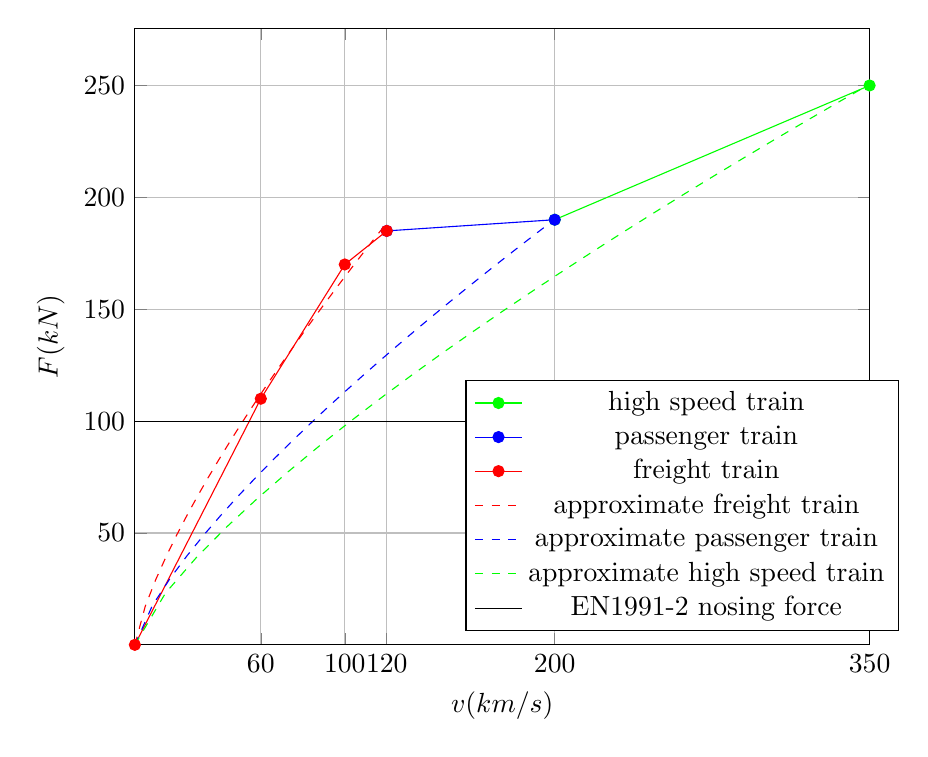
\begin{tikzpicture}
    \begin{axis}[
    % title = {Peak lateral track forces over all track qualities(worn profile scenario neglected)},
    width = 0.9\textwidth,
    xlabel={$v(km/s)$},
    ylabel={$F(kN)$},
    ymin = 0, xmin = 0, xmax = 350,
    grid = both,
    ytick = {50,100,...,250},
    xtick = {60,100,120,200,350},
    legend style={
    at={(0,0)},
    anchor=north west,at={(axis description cs:0.45,0.43)}}] 
    ]
    \addplot[name path = C,mark=*, green] coordinates {(200,190) (350,250)};
    \addplot[blue,name path = B,mark=*] coordinates {(120,185) (200,190)};
    \addplot[red,name path = A,mark=*] coordinates {(0,0) (60,110) (100,170) (120,185)};
    \addplot[red,name path = D, domain = 0:120, dashed]{5.2064*x^0.7498};
    \addplot[blue,name path = E, domain = 0:200, dashed]{3.58*x^0.7498};
    \addplot[name path = F, domain = 0:350, dashed, green]{3.1*x^0.7498};
    \addplot[domain = 0:350] {100};
    \legend{high speed train, passenger train, freight train, approximate freight train ,approximate passenger train, approximate high speed train, EN1991-2 nosing force},
    \end{axis}
\end{tikzpicture}
\caption{Total peak lateral track forces over all track qualities(worn profile scenario neglected)}
\label{fig:peaklateralforceregression}
\end{figure}

\paragraph{Evaluation on the peak lateral force model}
By examining the magnitude of forces illustrated in Figure.\ref{fig:peaklateralforceregression}, it is found that these forces are not reasonable because their magnitude is obviously too high.

The reason for this phenomenon is because the force data are extracted from simulations whose track quality ranges from well-maintained to very poor\footnote{Up to 6mm deviation}. Poor tracks result in extremely high lateral forces, however such tracks are not allowed in the Netherlands. 

The magnitude of forces can be calibrated if simulations based on realistic data of Dutch rails are provided. See Section.\ref{sec:recommendationsonsimulations} for recommendations on conducting simulations.


\subsection{Hypothesis expression for amplitude $Q$}

In this chapter a hypothesis expression for amplitude $Q$ is obtained. The hypothesis is based on \emph{peak lateral force model} in Section.\ref{sec:peaklateralforcemodel} and \emph{numerical simulation results}\footnote{All the numerical simulation results used in this chapter are extracted from a lateral force research\citep{d181dt329}. The correctness of these numerical simulations are verified during the research.}. 

The numerical simulations\citep[among Figure.C1,C2,...,C30]{d181dt329} used in this section successfully produced resonance between railway vehicle and bridge. Thus they are suitable for calculating the parameters of resonance model. Simulations used in this paragraph uses input from normal tracks and wheels data which is representative for British railway tracks and vehicles in 1990s. Thus although the peak lateral force model is very conservative, the amplitude determined based on representative simulations still generates reasonable results. 

There are two steps to create the hypothesis:

\begin{enumerate}
	\item Calculate the magnitude of $Q$ using inputs of different numerical simulation
	\item Make hypothesis based on calculated magnitude
\end{enumerate}
	
The following paragraphs of this section are written in above order.

\paragraph{Magnitude of $Q$} Inputs of 3 simulation cases are selected to calculate $Q$. They are abbreviated to C1,C3,C9\footnote{Abbreviations are used in following paragraphs to represent simulation cases } and presented in Figure.\ref{fig:c1},\ref{fig:c3} and \ref{fig:c9} respectively. $Q$ is calculated by substituting the peak displacement value of simulation output into the left hand side of the explicit solution and simulation inputs into right hand side of the same equation. With 3 sets of input and output data, 3 values of $Q$ are obtained. They are illustrated in Table.\ref{tab:parametersetupsandequivalentforce} together with the corresponding input data.


\begin{figure}[h!]
    \centering
    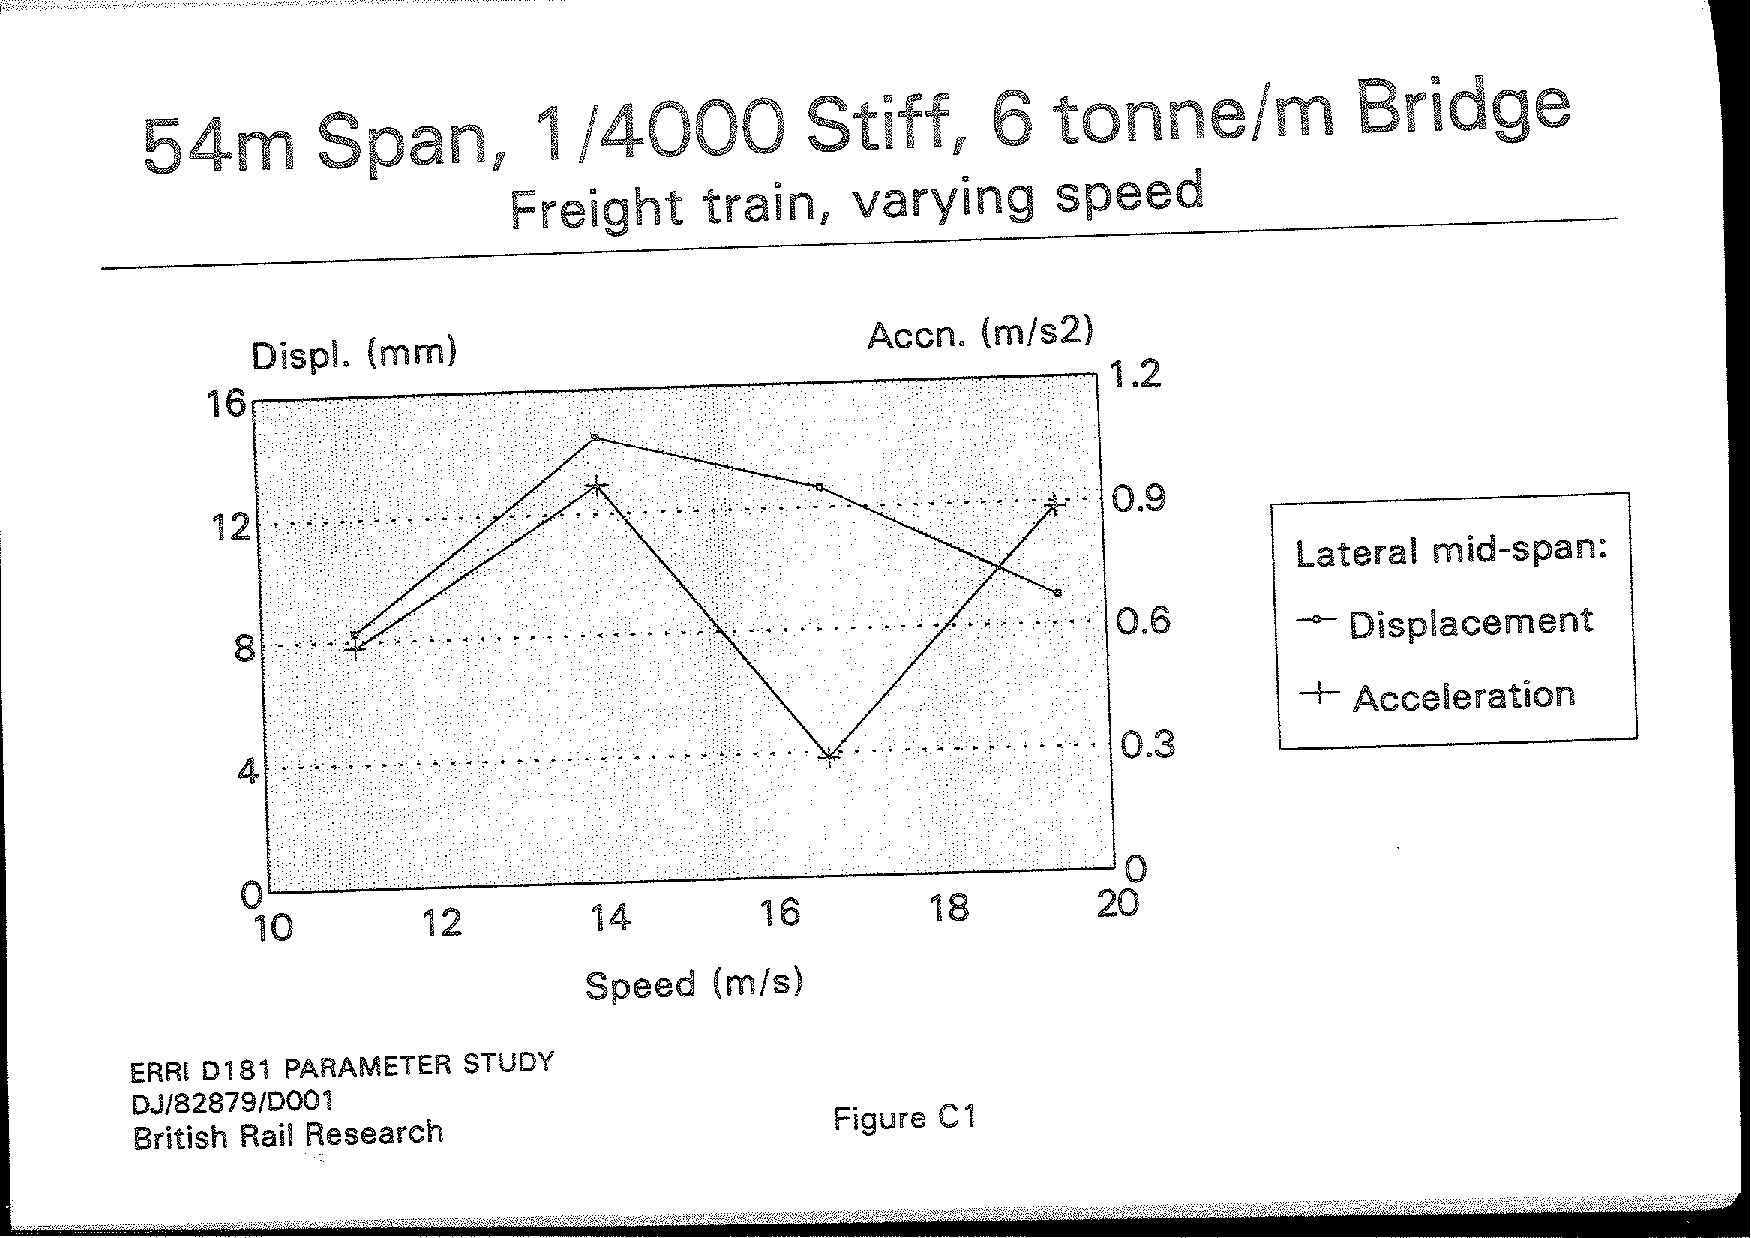
\includegraphics[height = 0.25\textheight]{c1}
    \caption{Figure C1 extracted from \citet{d181dt329} }
    \label{fig:c1}
\end{figure}

\begin{figure}[h!]
    \centering
    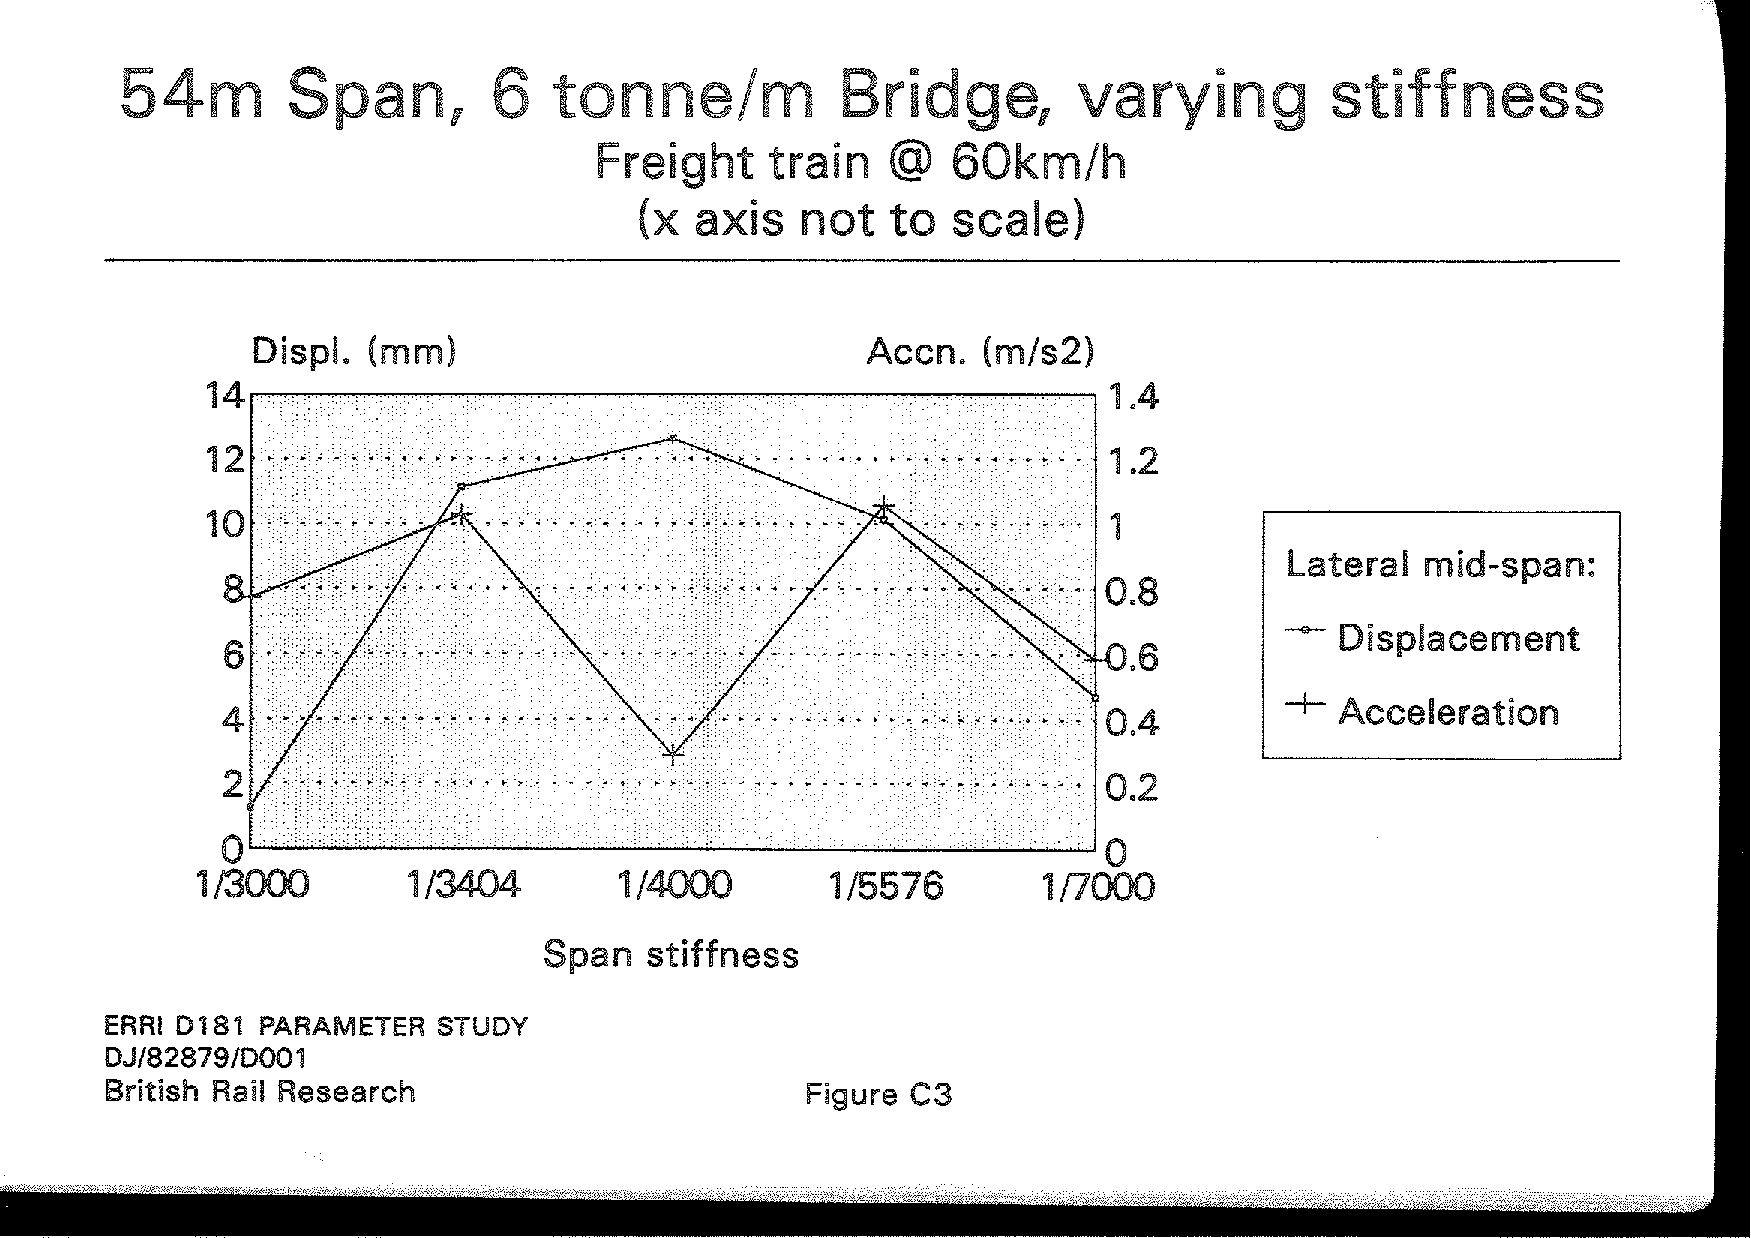
\includegraphics[height = 0.25\textheight]{c3}
    \caption{Figure C3 extracted from \citet{d181dt329} }
    \label{fig:c3}
\end{figure}



\begin{table}[ht!]
    \centering
    \caption{Parameter inputs and magnitude of amplitude $Q$}
    \begin{tabularx}{\textwidth}{c|XXX}
        \hline
        & \multicolumn{3}{c}{Simulation cases}  \\
        Parameters & C1 & C3 & C9 \\
        \hline
        $EJ$($\sfrac{\delta_0}{l}$) & 1/4000 & 1/4000 & 1/10000 \\
        $l$($m$) & 54m & 54 & 120 \\ 
        $\mu$($kg/m$) & 6000 & 6000 & 6000\\
        $c$($m/s$) & 14 & 16.67(60km/h) & 14\\
        $\zeta$ & 1\% & 1\% & 1\%\\
        Train  & Freight & Freight & Freight \\
        Track &  Freight  & Freight & Freight \\
        \hline
        Amplitude $Q$(kN) & 14 & 15 & 14 \\
        \hline
    \end{tabularx}
    \label{tab:parametersetupsandequivalentforce}
\end{table}

\paragraph{Hypothesis expression}By observing calculated magnitudes of amplitude $Q$, it is found that $Q$ possesses the general characteristics of peak lateral force model that the lateral force is only relevant to speed if track quality and wheel conicity are fixed. And lateral force is irrelevant to the bridge parameters.
 
Because amplitude $Q$ possesses the general lateral force characteristics, it is further expected that $Q$ also has a similar form of force-speed relationship as peak lateral force model. Thus hypothesis expression is created by scaling Eq.\ref{for:regressionfreight}. 

The exponential component does not change when scaling, so to scale the equation one set of input and output data is needed. Data $(Q = 14kN, c=14m/s)$ from C1 is selected. Please note only C1 was used in creating the hypothesis expression so C3 and C9 remains available for the verification.

The hypothesis expression for amplitude $Q$, which is the result of scaling, is presented in Eq.\ref{eq:hypothesisexpression}.

\begin{equation}\label{eq:hypothesisexpression}
    Q= 1928\times c^{0.7495}
\end{equation}

Please note that this hypothesis expression is created based on a specifically chosen simulation case C1. To be scientific, expression based on other simulations will be investigated in Section.\ref{sec:supplementaryparametercalculation}.

\section{Benchmark for the model}
Since amplitude $Q$ is a function of train speed $c$, the explicit solution is fully derived and only contains basic parameters. This sections aims to validate the capability of the explicit solution in yielding reasonable output.

New simulation cases\footnote{To assure conservativeness during the validation process, only axle repeat pattern resonance simulations are selected because their output are more pronounced than kinematic resonance effect.\citep{d181dt329}} C12,C13,C14\footnote{Abbreviation in original research. These abbreviation will continually be used in the following paragraphs.} are selected to take part in validation process. They are presented in Figure.\ref{fig:c12}, \ref{fig:c13} and \ref{fig:c14} respectively. As mentioned above, C3 and C9 are also available for the validation, therefore there are altogether 5 sets of simulation can be used for validation.

\begin{figure}[h!]
    \centering
    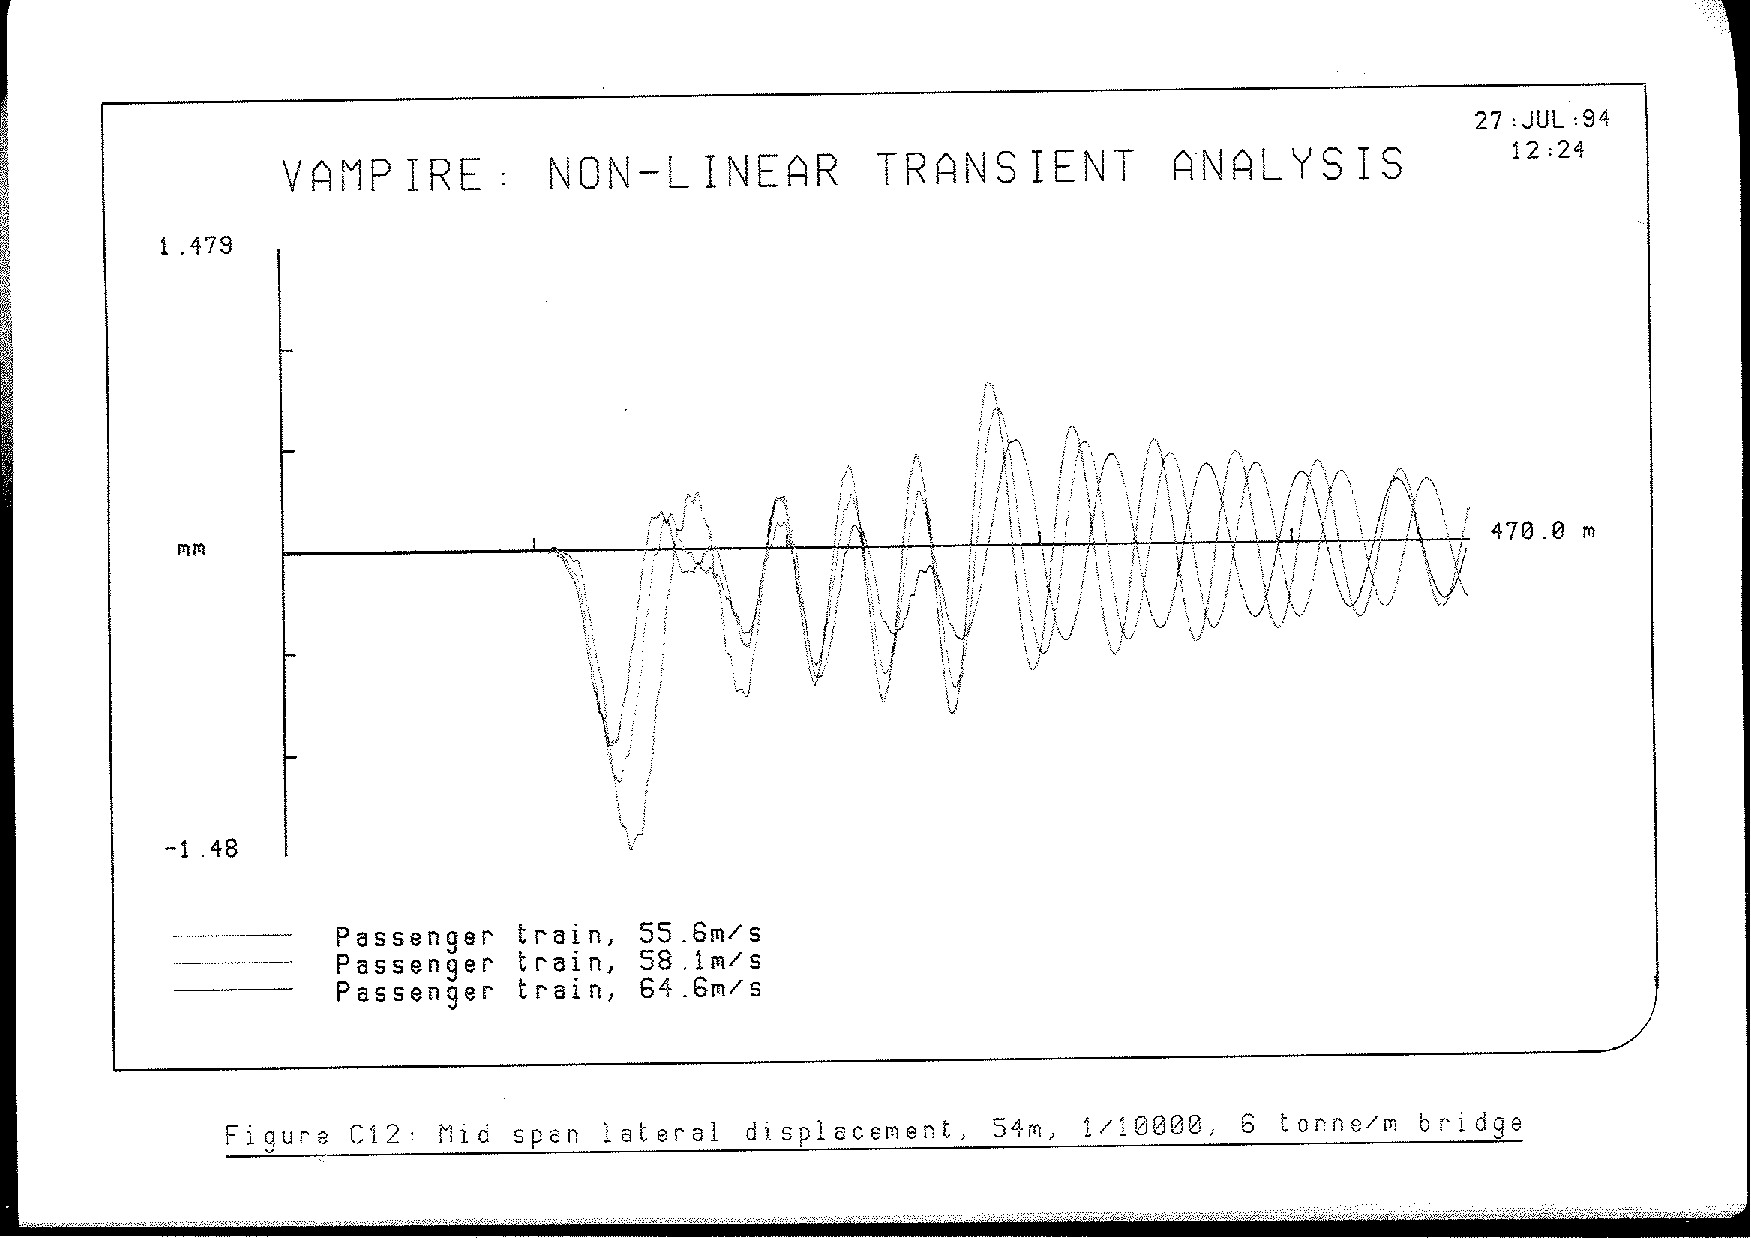
\includegraphics[height = 0.25\textheight]{c12}
    \caption{Figure C12 extracted from \citet{d181dt329} }
    \label{fig:c12}
\end{figure}

\begin{figure}[h!]
    \centering
    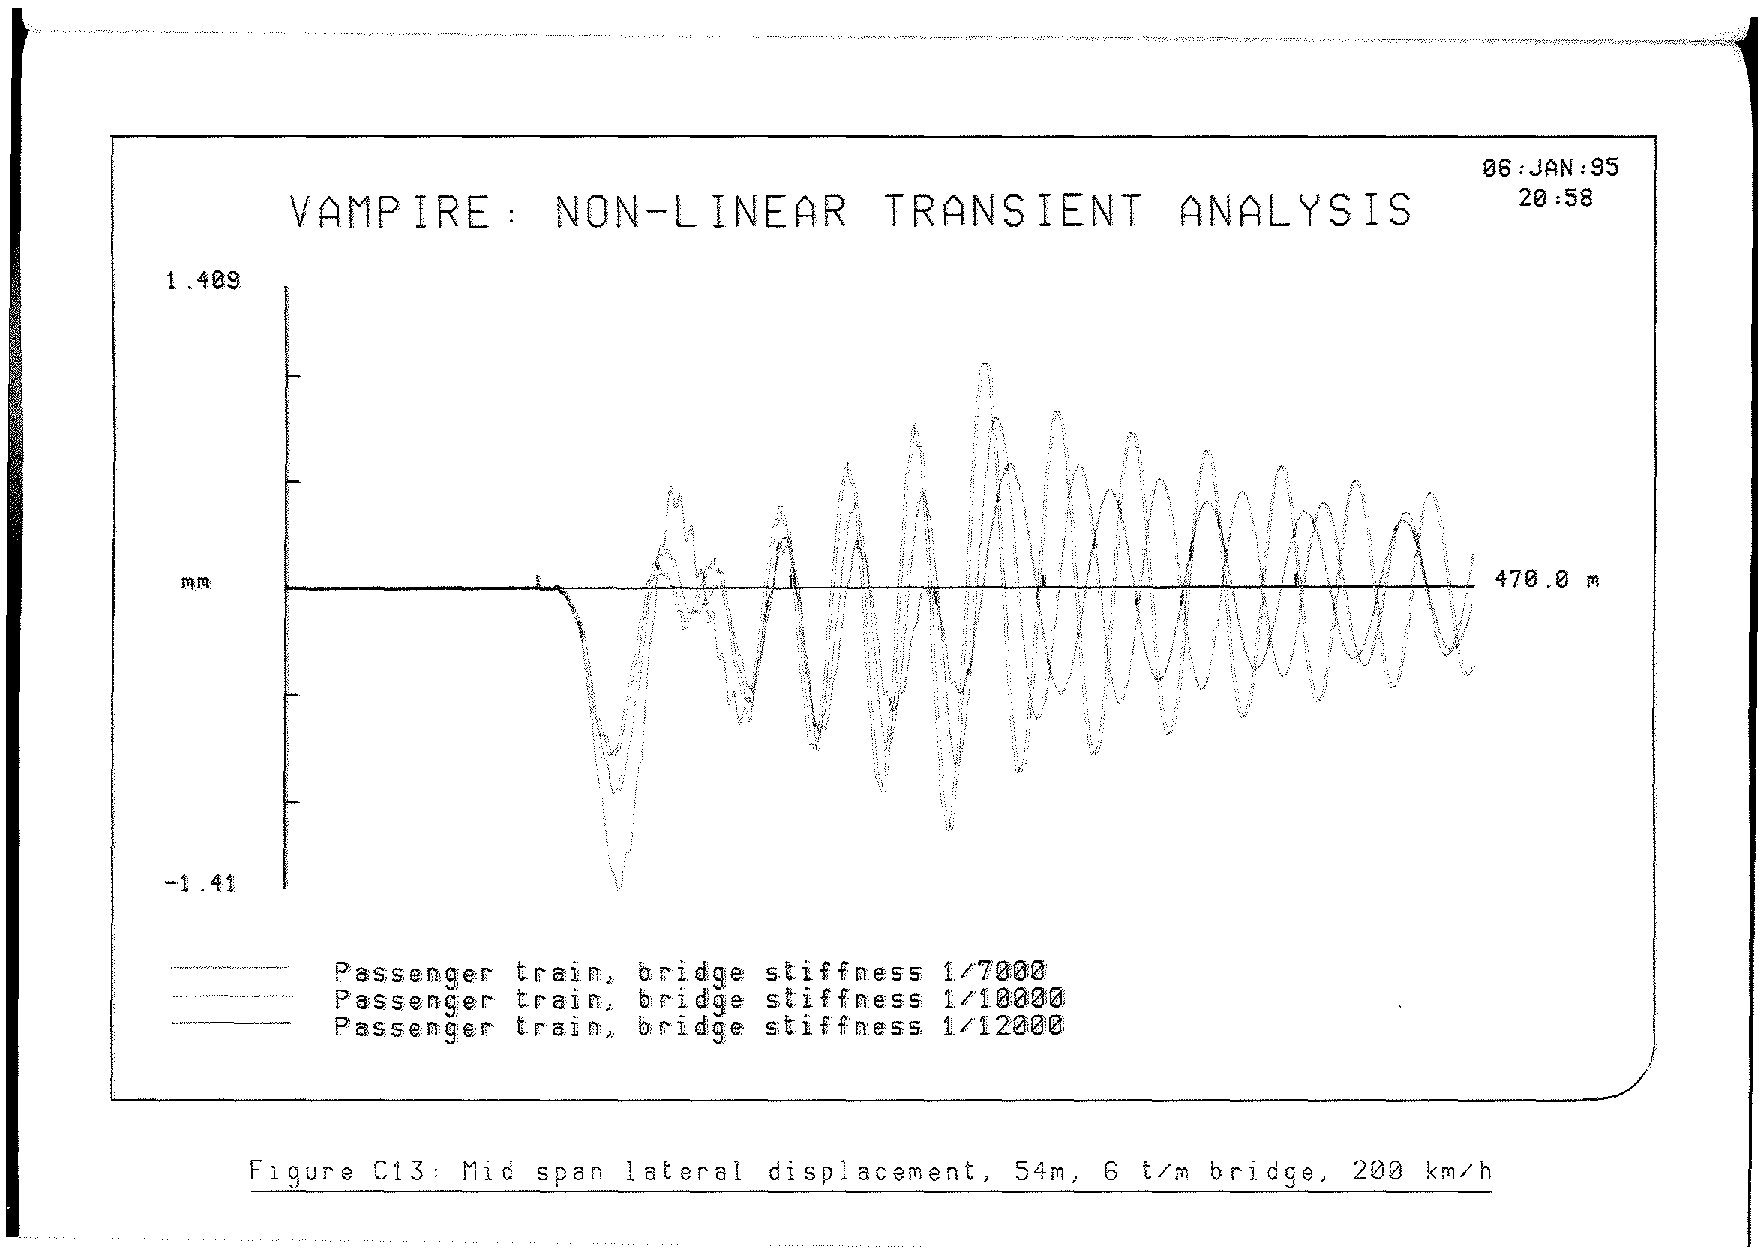
\includegraphics[height = 0.25\textheight]{c13}
    \caption{Figure C13 extracted from \citet{d181dt329} }
    \label{fig:c13}
\end{figure}

\begin{figure}[h!]
    \centering
    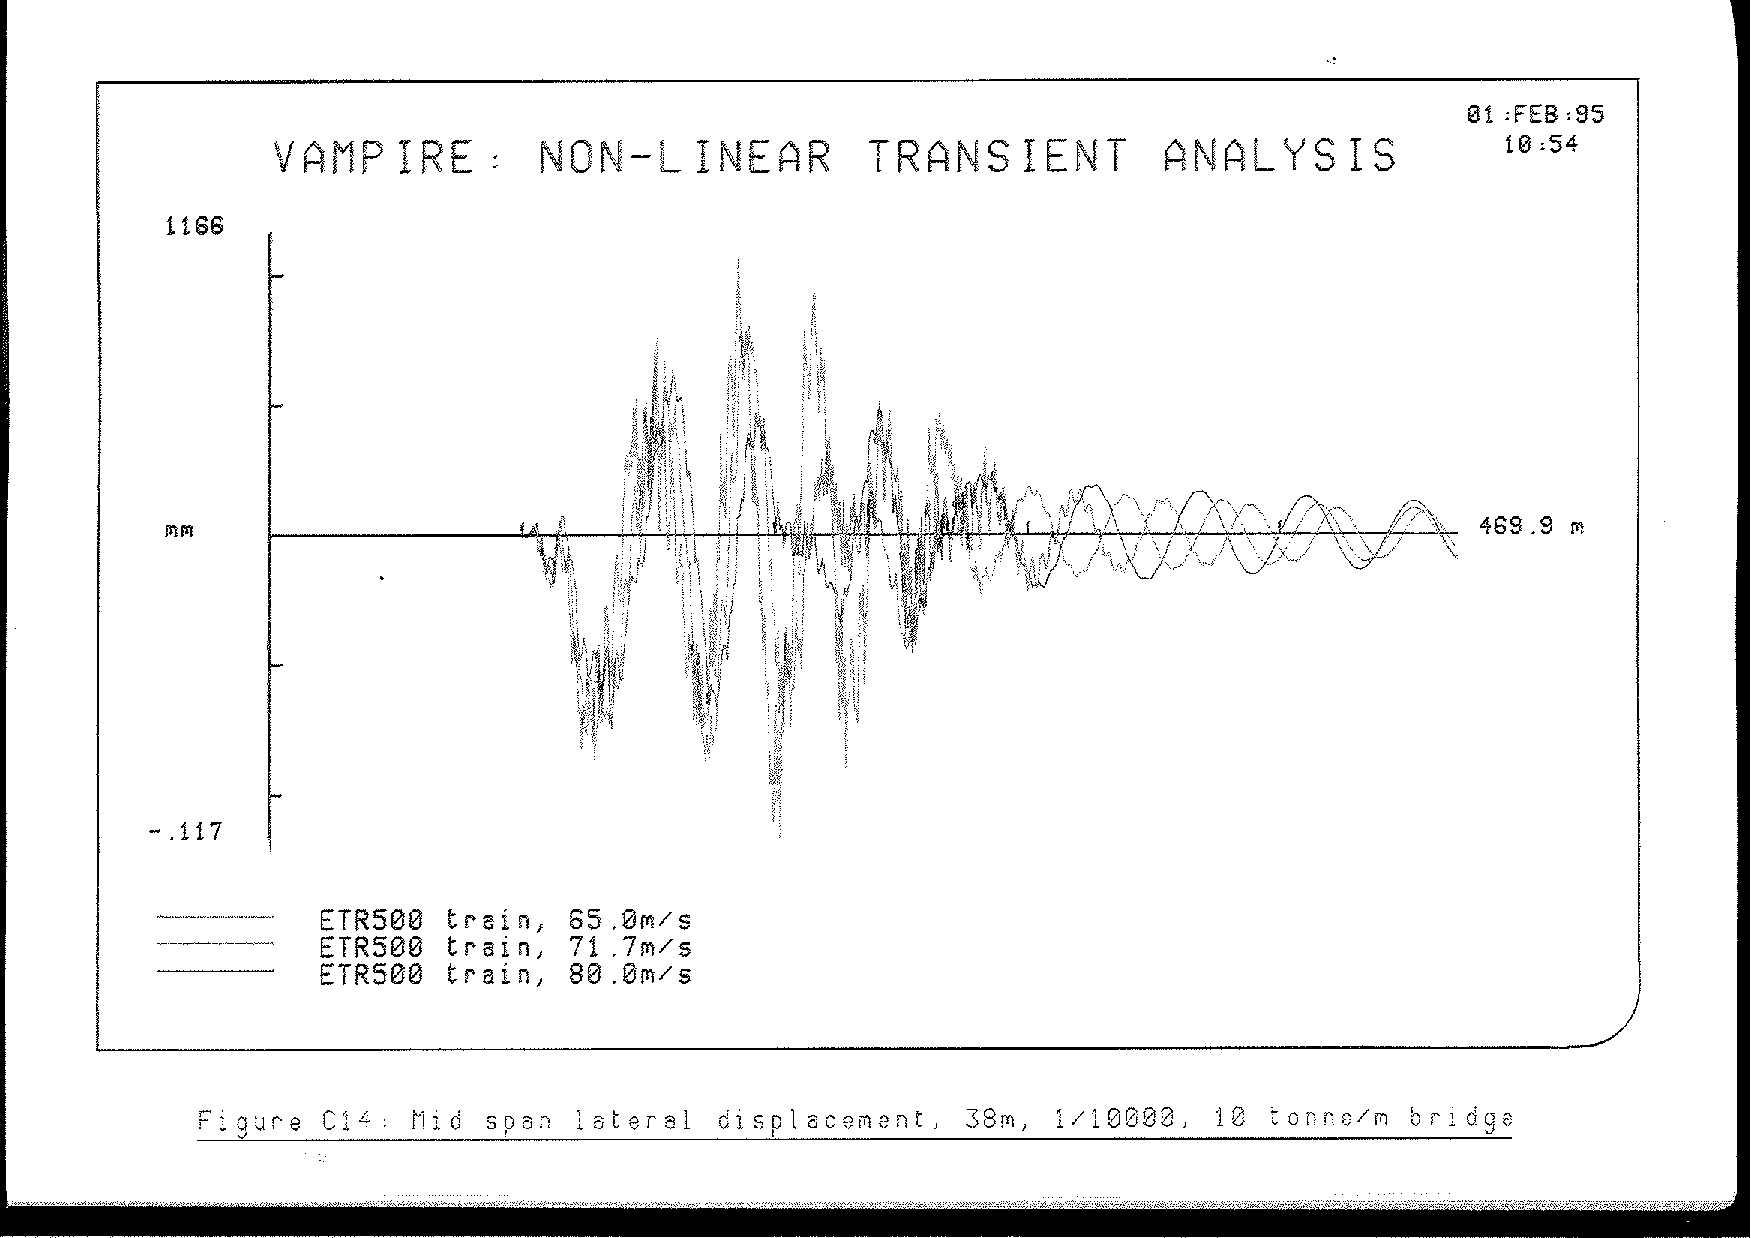
\includegraphics[height = 0.25\textheight]{c14}
    \caption{Figure C14 extracted from \citet{d181dt329}. An minor error is observed in y-axis label. Upper boundary of y-axis should be 0.116 }
    \label{fig:c14}
\end{figure}

The explicit solution is solved by inputing bridge parameters and trains speed of these 5 cases(C3,C9,C12,C13,C14). The results and their corresponding parameters are presented in Table.\ref{tab:comparisonresultssimulationanalytical}.

\begin{table}[h!]
    \centering
    \caption{Comparison of results of simulation output and analytical output using refined load model}
    \begin{tabularx}{\textwidth}{X|XXXXX}
        \hline
        & \multicolumn{5}{c}{Simulation cases} \\
        Parameters & C3 & C9 & C12 & C13 & C14\\
        \hline
        $EJ$($\sfrac{\delta_0}{t}$) &1/4000 & 1/10000& 1/10000 & 1/12000 & 1/10000\\
        $l$($m$) & 54 & 120 & 54 & 54 & 38\\
        $\mu$($kg/m$) & 6000 & 6000 & 6000 & 6000 & 10000\\
        $c$($m/s$) &16.67 & 14 & 55.6 & 55.6 & 65\\
        $\zeta$ & 1\% & 1\% & 1\% & 1\% & 1\%\\
        Train & Freight & Freight & Passenger & Passenger & High speed \\
        Track & Freight & Freight & Passenger  & Passenger  & High speed \\
        \hline
        PSD($mm$) & 12.5 & 17.8 & 1.48 & 1.41 & 0.117\\
        RES($mm$) & 14.1 & 19.7 & 6.6 & 5.8 & 3.0 \\
        \hline
    \end{tabularx}
    \begin{flushleft}
    	\vspace{0.5cm}
    	PSD: Peak simulation displacement \\
    	RES: Result of the explicit solution
    \end{flushleft}
    \label{tab:comparisonresultssimulationanalytical}
\end{table}

To clearer illustrate the comparison of both peak results from simulation and explicit solution, Figure.\ref{fig:comparisonpeaksimulationanalytical} is created with rearranged order to make descending trend more obvious.

\begin{figure}[h!]
\centering
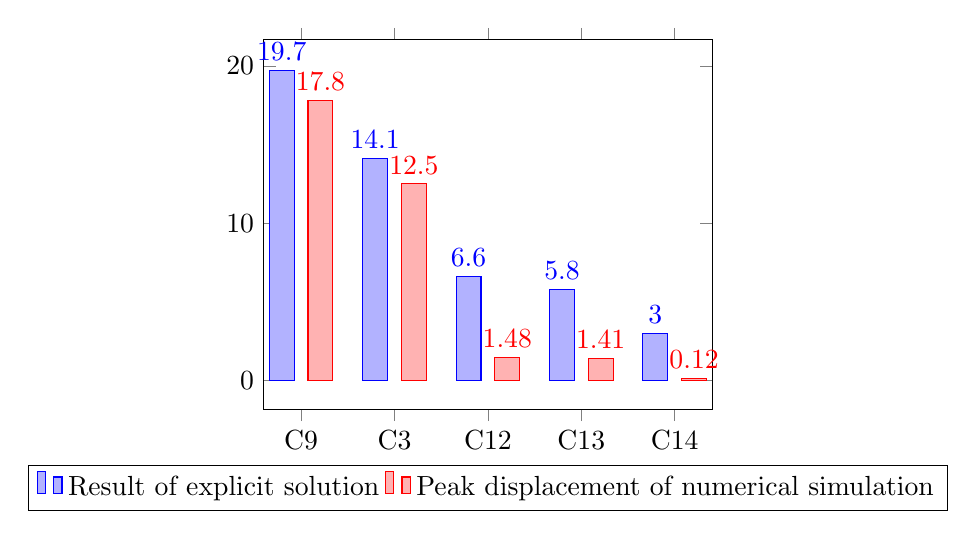
\begin{tikzpicture}
\begin{axis}[
	width = 0.6\textwidth,
    symbolic x coords={C9,C3,C12,C13,C14},
    xtick=data,
    legend style={at={(0.5,-0.15)},
        anchor=north,legend columns=-1},
    ybar=5pt,% configures `bar shift'
    bar width=9pt,
    nodes near coords,
]
\addplot 
    coordinates {(C9, 19.7) (C3, 14.1)   (C12,6.6) (C13,5.8) 
        (C14, 3.0) };
\addplot 
    coordinates {(C9, 17.8) (C3, 12.5)  (C12,1.48) (C13,1.41)
         (C14,0.117) };
\legend{Result of explicit solution,Peak displacement of numerical simulation}
\end{axis}
\end{tikzpicture}
\caption{Comparison between VAMPIRE peak simulation result and analytical peak result}
\label{fig:comparisonpeaksimulationanalytical}
\end{figure}

\paragraph{Benchmark conclusion}

It can be seen that explicit solution results always keep a conservative margin above the numerical simulation results. 

Difference between explicit solution and numerical simulation result for C12,C13 and C14 is bigger compared to difference for C9 and C3. It is due to the fact that the amplitude $Q$ is calculated based on freight train lateral forces and freight trains induce greater lateral force compared to passenger trains and high speed trains(See Figure.\ref{fig:peaklateralforceregression}).

The descending trend of explicit solution results follows the descending trend of numerical simulation results perfectly regardless of train types. 

Thus considering above reasons, the model shows satisfying performance. However, since there are few data available as benchmark, this model is still not verified for real-life application.

\section{Supplementary parameter calculation and benchmark}\label{sec:supplementaryparametercalculation}
Although the hypothesis expression based on C1 has been validated, this process is not generic because C1 is chosen specifically. To be scientific it is also necessary to derive expression of amplitude $Q$ based on other 5 simulation cases. 

The load equivalent amplitude of other 5 setups are calculated and their constant component are presented in the Table.\ref{tab:allLoadEquivalentAmplitude}. Their corresponding benchmarks are presented in Table.\ref{tab:allBenchmark}. Calculation processes are omitted because they are conducted in the same way as C1-based amplitude $Q$.

\begin{table}[h!]
    \centering
    \caption{Constant component of amplitude $Q$($N$) from all available setups}
    \begin{tabular}{cccccc}
        \hline
        C1 & C3 & C9 & C12 & C13 & C14 \\
        \hline
        1928 & 1721 & 1760 & 427 & 463 & 228 \\
        \hline
    \end{tabular}
    \label{tab:allLoadEquivalentAmplitude}
\end{table}

\begin{table}[h!]
	\tiny
    \centering
    \caption{Benchmark of explicit solution results}
    \begin{tabularx}{\textwidth}{XXXXXXX}
        \hline
         & \multicolumn{6}{c}{Analytical results of cases}\\
        \cline{2-7}
        Base simulation cases for $Q$ & C1 & C3 & C9 & C12 & C13 & C14 \\
        \hline
        C1 & 0.0145 & 0.0141 & 0.0197 & 0.0066 & 0.0058 & 0.003 \\
        C3 & 0.013 & 0.0125 & 0.0174 & 0.0059 & 0.0051 & 0.0036 \\
        C9 & 0.013 & 0.0128 & 0.0178 & 0.0061 & 0.0053 & 0.0032 \\
        C12 & 0.0032 & 0.0031 & 0.0043 & 0.00148 & 0.0013 & 0.0008 \\
        C13 & 0.0035 & 0.0034 & 0.0047 & 0.0016 & 0.00141 & 0.0002 \\
        C14 & 0.0021 & 0.0020 & 0.0028 & 0.0010 & 0.0008 & 0.00012 \\
        \hline
        Simulation Peak Displacement & 0.014 & 0.0125 & 0.0178 & 0.00148 & 0.00141 & 0.00012 \\
        \hline
        \label{tab:allBenchmark}
    \end{tabularx}
\end{table}

Among all amplitude $Q$, the one created from C1 is most satisfying because its outputs are all conservative towards numerical simulation output. Other  amplitude shows at least one nonconservative output. 

It can also be observed that the results of C12,C13 and C14 are unacceptable due to the reason that their output are too small compared to numerical simulation output . They can't predict reliable result for C1,C3 and C9.

Since there is few data available, it's meaningless to conduct further statistical procedures. The rest of the thesis will use amplitude $Q$ base C1 because it is conservative on all benchmark. 

\section{Evaluation on the model}
A simplified model for checking lateral resonance response of railway bridge is developed in this chapter. This model is capable of simulating a resonance scenario where the bridge is passed by a moving railway vehicle. However, several disadvantages of the current model should be noted:

\begin{enumerate}
	\item Only one concentrated force is modeled to represent the lateral dynamic effect induced by railway vehicle. It means the load in the model can not represent the distribution of vehicle axle forces. 
	\item Amplitude $Q$ is calculated based on a specifically chosen numerical simulation case. However, the aim of the model is to generically simulate vehicle-bridge response behavior, and such specifically choosing may be against this principle of generic.  
	\item The model is not fully validated because of the small quantity of available simulation results for validation. These simulation scenarios can not represent generic real-life scenarios.
	\item The model is not calibrated for modern Dutch railway because model parameter $Q$ is based on data generated by old railway vehicles.\footnote{Simulations\citep{d181dt329} were conducted during 1990s using parameters extracted from real trains at the time. Compared to trains of 1990s, modern railway vehicles possess more sophisticated suspension systems designed to suppress the lateral motion of the vehicle thus they are expected to induce lower lateral forces to tracks.} 
\end{enumerate}

%!TEX root = main.tex

\chapter{Practical usage of simplified model}

In practical usage, the speed that generates the highest peak response is unknown. Thus it is necessary to obtain the peak response for all speeds within the possible speed range. This is done by iteratively solving the explicit solution Eq.\ref{eq:v(x,t)simpleharmonic} with a speed range. The increment in speed iteration is set in a way that ensures at least 1000 runs are done to guarantee precession. An example is illustrated as follows to show the usage on a real bridge project.

A case study is done to illustrate the work flow in using the simplified model. Matlab scripts are written to automate the process. Scripts are presented in Appendix.\ref{sec:matlabscripts}.

\section{Case study}
For an arch railway bridge located near Amsterdam, first step to is to collect following parameters:

$L = 255m$, $m = 5222e3kg$, $\mu = 2.0478e4 kg/m$, $EJ = 6.56e12Nm^2$

where:

$L$: span of the bridge

$\mu$: uniform mass per unit length of the bridge

$EJ$: lateral stiffness of the bridge

to test through a speed range of $1m/s - 30m/s$

By inputting following command into Matlab console\footnote{Before beginning the calculation, make sure fog.m and Speedenvelop.m are in current working directory. }, 

\texttt{>>Speedenvelop(6.56e12,255,2.0478e4,1,30,0.01)}


the envelop for displacement is generated and illustrated in Figure.\ref{fig:spedefEJ6560000000000L255min1max30mu20478.tikz}

\begin{figure}[h!]
\centering 
% \newlength\figureheight 
% \newlength\figurewidth 
\setlength\figureheight{6cm} 
\setlength\figurewidth{6cm} 
% This file was created by matlab2tikz v0.4.7 (commit 29117077607177efe915cc01d961cced006239c8) running on MATLAB 8.3.
% Copyright (c) 2008--2014, Nico Schlmer <nico.schloemer@gmail.com>
% All rights reserved.
% Minimal pgfplots version: 1.3
% 
\begin{tikzpicture}

\begin{axis}[%
width=\figurewidth,
height=\figureheight,
scale only axis,
xmin=0,
xmax=30,
ymin=0.0075,
ymax=0.011,
title={SpeedEnvelop def from1 to30}
]
\addplot [color=blue,solid,forget plot]
  table[row sep=crcr]{%
1	0.00781568842060085\\
1.2	0.00840892567977264\\
1.4	0.0088768875903958\\
1.6	0.00925769529057003\\
1.8	0.00957910144655464\\
2	0.00982648840148397\\
2.2	0.0100372557099215\\
2.4	0.0102060089657038\\
2.6	0.010347841028453\\
2.8	0.0104753362289414\\
3	0.010566090236029\\
3.2	0.0106426943938749\\
3.4	0.0107156879259678\\
3.6	0.0107656368912521\\
3.8	0.0108134770961416\\
4	0.0108433829006734\\
4.2	0.0108762461970553\\
4.4	0.0109009754438711\\
4.6	0.0109137058875431\\
4.8	0.0109063964703489\\
5	0.0109283926778865\\
5.2	0.0109354115709882\\
5.4	0.010934364378216\\
5.6	0.010925358882146\\
5.8	0.0109155184260617\\
6	0.0109160952245694\\
6.2	0.0109022893020932\\
6.4	0.0108894990281659\\
6.6	0.0108791296950589\\
6.8	0.0108683159097076\\
7	0.0108485530748728\\
7.2	0.0108354499334163\\
7.4	0.0108143121429067\\
7.6	0.0107967054438007\\
7.8	0.0107826189027167\\
8	0.0107571129205081\\
8.2	0.0107450192698353\\
8.4	0.0107182431373167\\
8.6	0.0107081009100856\\
8.8	0.0106810097968274\\
9	0.0106647893596357\\
9.2	0.0106368269751327\\
9.4	0.0106244435627288\\
9.6	0.0105902161380316\\
9.8	0.0105787489298167\\
10	0.0105530497685275\\
10.2	0.0105311301588914\\
10.4	0.0105155111529359\\
10.6	0.0104818416711415\\
10.8	0.0104658192794055\\
11	0.0104515232844051\\
11.2	0.0104195968460413\\
11.4	0.0103992383576141\\
11.6	0.0103875827376142\\
11.8	0.0103585518798102\\
12	0.0103282987036047\\
12.2	0.0103183620397562\\
12.4	0.0103012474040927\\
12.6	0.0102668977746374\\
12.8	0.0102449204320541\\
13	0.0102354809790005\\
13.2	0.0102169579397151\\
13.4	0.0101865143682396\\
13.6	0.0101530378665145\\
13.8	0.0101488592884028\\
14	0.0101342026283539\\
14.2	0.0101129828210581\\
14.4	0.0100781640001081\\
14.6	0.010051230942275\\
14.8	0.0100463931273211\\
15	0.0100339102223161\\
15.2	0.0100154789040376\\
15.4	0.00998674150551577\\
15.6	0.00995047989615967\\
15.8	0.00993544019804088\\
16	0.00993088834100722\\
16.2	0.0099199018939231\\
16.4	0.00990104705345698\\
16.6	0.00987441551082942\\
16.8	0.00984237739719204\\
17	0.00980928040956712\\
17.2	0.0098093242438416\\
17.4	0.00980329783311577\\
17.6	0.00979122702961792\\
17.8	0.00977314390458511\\
18	0.00974908670711774\\
18.2	0.00972108217302529\\
18.4	0.0096776691907686\\
18.6	0.00966812567615805\\
18.8	0.0096672743699076\\
19	0.00966167442250244\\
19.2	0.00965133478148734\\
19.4	0.00963626874305325\\
19.6	0.00961649393213872\\
19.8	0.00959203227865456\\
20	0.00956290998985286\\
20.2	0.0095021185042862\\
20.4	0.00950695108828918\\
20.6	0.00950797086177456\\
20.8	0.00950518266938973\\
21	0.00949859410737403\\
21.2	0.00948821551471712\\
21.4	0.00947405996230233\\
21.6	0.00945635016311157\\
21.8	0.00943490732597904\\
22	0.00940971735699768\\
22.2	0.00931048059107463\\
22.4	0.00931929357671497\\
22.6	0.00932536783564737\\
22.8	0.00932827887006457\\
23	0.00932803971339443\\
23.2	0.00932466491318731\\
23.4	0.00931817052503146\\
23.6	0.00930857410555171\\
23.8	0.00929589470449585\\
24	0.0092803683442182\\
24.2	0.00926243390849551\\
24.4	0.0092414380792758\\
24.6	0.00916278336234724\\
24.8	0.00909609061802426\\
25	0.00910564521095271\\
25.2	0.00911382028447303\\
25.4	0.00911959836984988\\
25.6	0.00912274595493189\\
25.8	0.00912328389307619\\
26	0.00912136767440461\\
26.2	0.00911807810466714\\
26.4	0.00911219402539695\\
26.6	0.00910373969614448\\
26.8	0.0090927400294876\\
27	0.00907945686157787\\
27.2	0.00906461860626204\\
27.4	0.00904726523290454\\
27.6	0.00902380873477224\\
27.8	0.00882644457839617\\
28	0.00883996385182427\\
28.2	0.00885231633946435\\
28.4	0.00886244919403873\\
28.6	0.00887051931610704\\
28.8	0.00887784576510649\\
29	0.0088829756466977\\
29.2	0.00888593368675971\\
29.4	0.00888785865101469\\
29.6	0.00888798738354364\\
29.8	0.00888597303168551\\
30	0.00888235391855735\\
};
\end{axis}
\end{tikzpicture}% 
\caption{Peak deflection at mid-span with regard to changing train speed. Parameters: $EJ = 6.56e12Nm^2$, $L= 255m$,$\mu = 20478 kg/m$, $c_{min}=1m/s$, $c_{max} = 30m/s$} 
\label{fig:spedefEJ6560000000000L255min1max30mu20478.tikz} 
\end{figure}

The plot shows that the critical speed appears at approximately $5m/s$ and corresponding peak deflection response is approximately $11mm$. 

Since the relationship between end support rotation angle and mid-span deflection is widely known as:

$$ \varphi = \frac{3}{L}\cdot \delta_0  $$

and rotation is yielded as:

$$ \varphi = \frac{3}{255}\times 0.011 = 0.00013 $$

This value is much lower than the rotation value regulated in EN1991-2. See Section.\ref{sec:Transverse-deformations-and-vibrations} for criteria details.

Thus the conclusion can be made that this bridge is safe subjected to lateral dynamic load.

\section{Conclusion}

A general conclusion of practical method is, for a certain bridge, faster train speed does not necessary result in higher resonance response of the bridge. As can be seen in Figure.\ref{fig:spedefEJ6560000000000L255min1max30mu20478.tikz}, critical speed appears at approximately $5m/s$, and response start to fall when speed is higher than $5m/s$. This means comparing to higher load amplitude caused by higher train speed, the shorter loading time caused by same reason is more dominating. By considering the fact in Figure.\ref{fig:comparisonpeaksimulationanalytical} that the explicit solution is even more conservative for higher speed. Tt can be concluded that high-speed trains cause less dynamic problem for lateral bridge dynamics.

Matlab scripts are already written and attached for the convenience of designers. Since the explicit solution has been given in the chapter, it's completely possible to adopt them in other mathematical software for different preferences.

%!TEX root = main.tex

\chapter{Conclusion}

This thesis successfully fulfilled the required tasks in the research objectives and question.

To assist the design of a long-span bridge of Iv-infra, a simplified model for assessing lateral bridge resonance behavior is developed in this thesis. This model is validated to be conservative and reasonable by benchmark. 

However, due to the lack of data available in creating the model, the model is not validated to be applied universally on real-life project. Currently it has following disadvantages:

\begin{enumerate}
	\item Only one concentrated force is modeled to represent the lateral dynamic effect induced by railway vehicle. It means the load in the model can not represent the distribution of vehicle axle forces. 
	\item Amplitude $Q$ is calculated based on a specifically chosen numerical simulation case. However, the aim of the model is to generically simulate vehicle-bridge response behavior, and such specifically choosing may be against this principle of generic.  
	\item The model is not fully validated because of the small quantity of available simulation results for validation. These simulation scenarios can not represent generic real-life scenarios.
	\item The model is not calibrated for modern Dutch railway because model parameter $Q$ is based on data generated by old railway vehicles.\footnote{Simulations\citep{d181dt329} were conducted during 1990s using parameters extracted from real trains at the time. Compared to trains of 1990s, modern railway vehicles possess more sophisticated suspension systems designed to suppress the lateral motion of the vehicle thus they are expected to induce lower lateral forces to tracks.} 
	\item The longest bridge in numerical simulation is 120m long. Thus the model is not validated for bridges longer than 120m.
\end{enumerate}

Despite the disadvantages of the current model, it provides a direction of analyzing lateral dynamics of railway bridges which is different from nowadays available analyzing techniques. It offers a simple approach to avoid heavy numerical simulations during the analysis and therefore, saves the effort and cost for designers. The model shall be regarded as a prototype that can be improved and expanded by future researches. See Chapter.\ref{sec:recommendations} for details of recommendations for future researches.

%!TEX root = main.tex

\chapter{Recommendations for future researches}\label{sec:recommendations}

The recommendations aims to guide future researches to be conducted according to the disadvantages mentioned in previous chapter.

General recommendations:

\begin{enumerate}
	\item Improve the model by make more sophisticated assumption to better reflect real-life scenario. For example: use more than one concentrated force to represent the lateral dynamic load. 
	\item It is recommended to use a larger database when determining the expression for parameters.
	\item Conduct more numerical simulations to provide database for the sake of creation and validation of the model. See Section.\ref{sec:recommendationsonsimulations} for detailed explanation on how to conduct these simulations.
\end{enumerate}

\section{Recommendations on numerical simulations}\label{sec:recommendationsonsimulations}

More accurate statistical result can be yielded with more simulation data. Since now only 6 sets of data are used, the simplified model is not globally reliable. However, it is recommended that future research uses a larger simulation data base to further improve the accuracy of the model.

It is possible to modify the amplitude of the model to a less conservative value according to newly conducted simulations. It is expected that newly conducted simulations yield smaller lateral force on tracks because of the advanced suspension systems implemented in modern vehicle designs and better track quality.

Therefore, numerical simulations are recommended to be conducted according to following suggestions:

\begin{enumerate}
    \item Use more realistic and up-to-date data on modern Dutch train vehicles and railway. The result will help the model to be applicable for Dutch bridges.
    \item Investigate over a broader range of bridge span(greater than 150m).
\end{enumerate}



% %!TEX root = main.tex

\chapter{Criteria regarding lateral railway bridge dynamics included in EN1991-2 and their origins}\label{Chap:selectedCriteria}

In this chapter, firstly, several criteria regarding lateral railway bridge dynamics included in Eurocode EN1991-2 are selected. The reason for the selection is that the selected criteria tend to causing inevitable violation for modern long-span railway bridge designs. 

Then, in order to assess the feasibility and the reliability of the selected criteria, their origin were traced and interpreted. By interpreting the original intension during the creation process of these selected criteria, assessment and remarks can be conducted further on.

Also, within the original research paper, more useful information can be extracted. These information can contribute to further improvement of the criteria or the creation of new validation method.

\section{Selected criteria}

Altogether two criteria were found in EN1991-2 with regard to lateral railway bridge dynamics. They are:

\begin{enumerate}
	\item 1.2Hz Criterion
	\item Nosing force
\end{enumerate}

\subsection{1.2Hz Criterion}
1.2 Hz criterion is defined in \citet[A24.4.2.4]{EC12} with following statement:

\begin{quote}
	...

	\textbf{The first natural frequency of lateral vibration of a span should not be less than $f_{h0}$. The value for $f_{h0}$ may be defined in the National Annex. The recommended value is: $f_{h0}=1.2 Hz$}

	...

\end{quote}

This criteria rejects almost all bridge designs that have span longer than 150m. This is due to the reason that longer span bridges possess lower lateral natural frequency. When the span is over 150m, normally the lateral natural frequency of the bridge fall below 1.2Hz. 

\subsection{Nosing force}\label{sec:nosingforce}
Nosing force is defined in Eurocode 1991-2. 

The characteristic value of the nosing force shall be taken as $Q_{sk} = 100kN$. It shall not be multiplied by the factor $\Phi$ (\citet[6.45]{EC12}) or by the factor $f$ in \citet[6.51]{EC12}. 

The characteristic value of the nosing force should be multiplied by the factor $\alpha$ in accordance with \citet[6.3.2]{EC12} for values of $\alpha \geq 1$

The nosing force shall always be combined with a vertical traffic load.


\subsection{Origins of selected criteria}
The selected criteria shares the same original research project conducted by ERRI(former UIC). The project is called: \textit{D181: Lateral forces on railway bridges}. 

\paragraph{Origin of 1.2Hz Criterion}
Its original proposal can be found in \citet[Proposed criteria]{d181}. The evidence of the this statement is that both definition use almost the same language. The original one explained the reason for choosing 1.2Hz frequency but EN1991-2 omitted the reason for choosing. The original definition is extracted as following for reference:

\begin{quote}
	To avoid the occurrence of resonance in the lateral motion of the vehicles due to the lateral motion of the bridge, a limit value lower than the first natural frequency $f_1t$ of the lateral vibration of the span studied should be fixed. The natural frequency for lateral movements is between 0.5 and 0.7 Hz for coaches and between 0.7 and 1 Hz for locomotives. We therefore propose a safety margin $F_{lt} \geq 1.2Hz$
\end{quote}

\paragraph{Origin of nosing force}
Its original background can be found in \citet[Proposed criteria]{d181}. It is defined as a representation of actions, in combine with actions like vertical loads, dynamic effects, centrifugal forces, traction and braking forces, etc.

The evidence of RP6 is the background of nosing force in EN1991-2 is the following repeating literature:

In \citet[6.5.2]{EC12}:
\begin{quote}
	(1)P The nosing force shall be taken as a concentrated force acting horizontally, at the top of the rails, perpendicular to the centre-line of track. It shall be applied on both straight track....
\end{quote}

In \citet[4.1B]{d181}:
\begin{quote}
	These forces shall be applied at the top of the rails in the most unfavourable position and acting horizontally, perpendicular to the track centreline...
\end{quote}

With another statement also helps proofing RP6 is the background of nosing force in EN1991-2 in \citet[4:Draft Recommendations]{d181}:

\begin{quote}
	These can therefore be expressed as follows: (Article \textbf{6.5.2} of ENV 1991-3 of 1994)...
\end{quote}

ENV 1991-3 was renamed to EN 1991-2 in 2003.

Originally in \citet[4:Draft Recommendations]{d181}, nosing forces was defined as lateral forces from vehicle/bridge interaction as a result of \textbf{hunting}.

\section{Conclusion}
Since all criteria regarding lateral railway bridge dynamics come from the same research project: \textit{D181:Lateral Forces on Railway Bridges}, it's essential to interpret the whole report series in order to have a better understanding on its proposed criteria. Next chapter will lay emphasis on interpreting and in the end, conduct assessment on the criteria.


\chapter{Interpretation of report series created by D181 Committee Group}\label{sec:D181reportseries}


\section{Introduction}

This chapter aims to interpret several key documents within the research report series D181. The interpreted documents contains relative contents to the problem-causing criteria filtered out already in Chapter.\ref{Chap:selectedCriteria}.

D181 Committee Group is created by UIC, in order to investigate Lateral Forces on Railway Bridges. Some of the proposed criteria in reports created by this committee group are adopted by Eurocode Committee to created Eurocode 1991-2. The goal of this interpretation is to summarize the research done by D181 report series and and give further conclusion.

The interpretation will be done in following aspects:

\begin{enumerate}
    \item Interpretation of DT329
    \item Interpretation of RP6
    \item Conclusion of D181 report series
\end{enumerate}

In this thesis document DT 329 and document RP 6 are obtained and studied, but other reports in English version are not available to the researcher.
For an overview of structure of report series, please refer to Appendix.\ref{app:generalInformationD181}.

\section{Items of interests in report series}

\begin{enumerate}
    \item Resonance mechanisms studied. They are discussed in DT329. See Section.\ref{sec:resonance329}
    \item The proposed 1.2 Hz Criterion and its background. It is discussed in RP6. See Section.\ref{sec:1.2criterion329}
    \item  Lateral forces(Nosing force) on the bridges. See Section.\ref{sec:lateralforce329}
\end{enumerate}


\section{Methodology of Parametric Research DT329}

The DT329 research was conducted in two phases. It is noted that all studies were done using VAMPIRE software. The reliability of simulation has been discussed and confirmed in a previous report of \citet{d181rp2}.

In the initial phase 11 sets of bridge parameters were selected for the simulation. 52 combinations of bridge parameters and train configurations were examined. The goal of the initial phase is to filter out most influencing parameters for bridge dynamics.

In the secondary phase, the influence of selected parameters were categorized into 3 cases. They include:
\begin{enumerate}
 \item the influence of multiple span bridges (viaducts)
 \item the influence of track quality
 \item the influence of stiffness/span/frequency on the resonant behaviour of the bridge
\end{enumerate}
They were studied by using the same simulation method used in initial research phase.


\section{Interpretation of resonance phenomenon studied in DT329}\label{sec:resonance329}

2 types of resonance were studied in DT329, including:

\begin{enumerate}
    \item Resonance caused by axle repeat pattern
    \item Resonance caused by kinematic movement
\end{enumerate}

The summary of these resonances effects are presented in following paragraphs. 

Frequency shift phenomenon is an important characteristics observed from resonance effects lists above. It is explained in Section \ref{sec:apparentshift}

\subsubsection{Resonance caused by axle repeat pattern}

Axle repeat patterns are wavelength phenomena - regardless of vehicle speed, the repeat length is constant. However, since frequency is speed divided by wavelength, the frequency of the axle repeat patterns vary with train speed. A table of axle repeat pattern lengths, and typical frequencies arising from train speed are given in Figure.\ref{tab:329axlerepeat}

By running train at different speeds shows resonance is possible between train and bridge if the axle passing frequency coincides with the first lateral bridge mode. The effect occurring in bridge lateral displacement over a limited frequency range around the resonance frequency.


However, the speed on theory which should yield resonance effect may be different from the speed that actually triggered resonance.

\subsubsection{Resonance caused by kinematic movement of trains} 
Kinematic wavelength also gives rise to frequencies which vary with speed for the same reason. For first lateral bending mode coincidence with kinematic frequency, the kinematic wavelength of each train type had to be established, by running each train at a range of typical operating speeds over a discrete lateral irregularity, and examining the frequency content of the lateral wheel motion. The resulting wavelength ranges are tabulated in Table.\ref{tab:329kinematicwavelength}. See Figure \ref{fig:workflow329kinematic} for an overview of workflow of this study.

The most likely possible resonance in the initial studies to be of this type was between the passenger train at 200 km/h (55.556 m/s) on passenger track and BR PI wheel profiles, and a span of 54 m, stiffness 1/10000, mass/length of 6 tonnes/m. This combination was examined by varying the speed between 55.556 - 64.6 m/s over the span, and by varying the stiffness of the span between 117000 and 1112000 running the train at 55.556 m/s. Another combination was examined - the ETR500 train running between 65 - 80 m/s on high speed track and BR PI wheel profiles, for a span of 38 m, stiffness 1110000, and mass/length 10 tonne/m; the span in this case was chosen to coincide with the kinematic wavelength of the coaches.

Coincidence of vehicle kinematic frequency with bridge first lateral bending mode may cause resonance to occur over a broad range of frequencies to a less pronounced effect than coincidence of axle passing frequencies. Evidence of coincidence of kinematic wavelength with length of span has been found in the lateral acceleration of bridges, but was not demonstrated in the lateral bridge displacement in the cases examined. For short kinematic wavelengths, this effect could not be seen, possibly because of lack of time for the bridge to respond.


\begin{figure}[h]
\centering
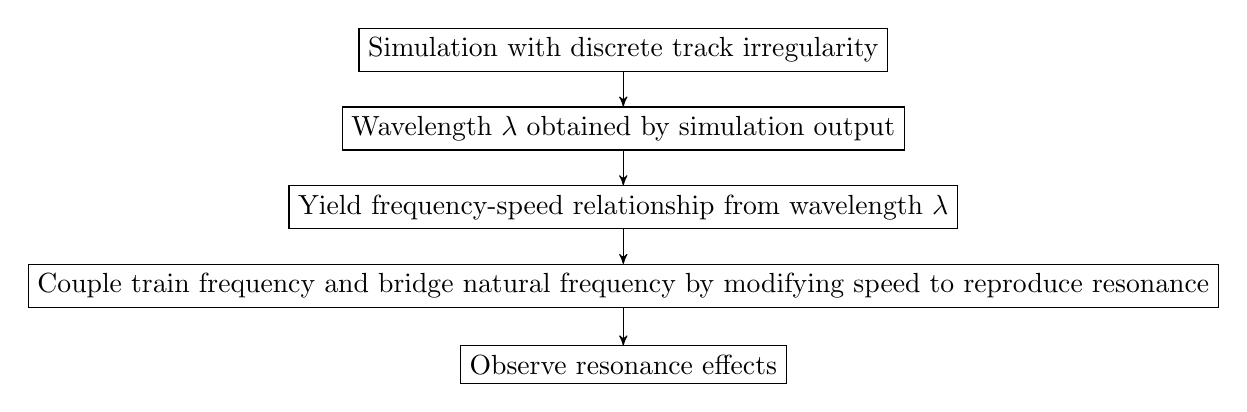
\begin{tikzpicture}
    \node[draw] (simulation1) at (0, 0) {Simulation with discrete track irregularity};

    \node[draw] (analysis) at (0, -1) {Wavelength $\lambda$ obtained by simulation output};

    \node[draw] (yielding) at (0, -2) {Yield frequency-speed relationship from wavelength $\lambda$};

    \node[draw] (matching) at (0,-3) {Couple train frequency and bridge natural frequency by modifying speed to reproduce resonance};

    \node[draw] (observe) at (0, -4) {Observe resonance effects};

    \draw[->] (simulation1) to (analysis);

    \draw[->] (analysis) to (yielding);

    \draw[->] (yielding) to (matching);

    \draw[->] (matching) to (observe);
\end{tikzpicture}
\caption{Workflow of kinematic resonance research}
\label{fig:workflow329kinematic}
\end{figure}

\subsubsection{Apparent shift in resonance frequency}\label{sec:apparentshift}
It is frequently observed in the output of both resonance effects that apparent resonance happens at some frequencies higher than frequencies calculated on theory. This is explained in following quote on \citet[Page 13, Secondary Phase]{d181dt329}. However, the explanation wasn't verified by further studies. They can only be treated as hypothesis.

\begin{quote}
Although the peak mid span displacement was expected to occur at 28.5 mis, it can be seen that for the runs with just the coaches that the peak occurs at about 32 m/s. This is confirmed to be a resonance-type effect rather than a discrete event in the time histories of the runs, a selection of which are shown in Figure C6(Original report), of which an extract of 100-285m follows as Figure C7(Original report). This speed is mid way between axle passing frequency coinciding with first bending mode of the bridge, and kinematic frequency coinciding with the first bending mode. So, the apparent shift in resonant frequency may be due to a combination of these effects (see discussion of kinematic frequency resonance results). However, an alternative explanation may be that as track forces generally increase with speed, the deflection of the span would be expected to increase. If this effect continued through a resonant band, the peak displacement would appear greater at a speed slightly above that calculated for resonance, as sketched in Figure \ref{fig:apparentshift}.
\end{quote}

\begin{figure}[h]
    \centering
    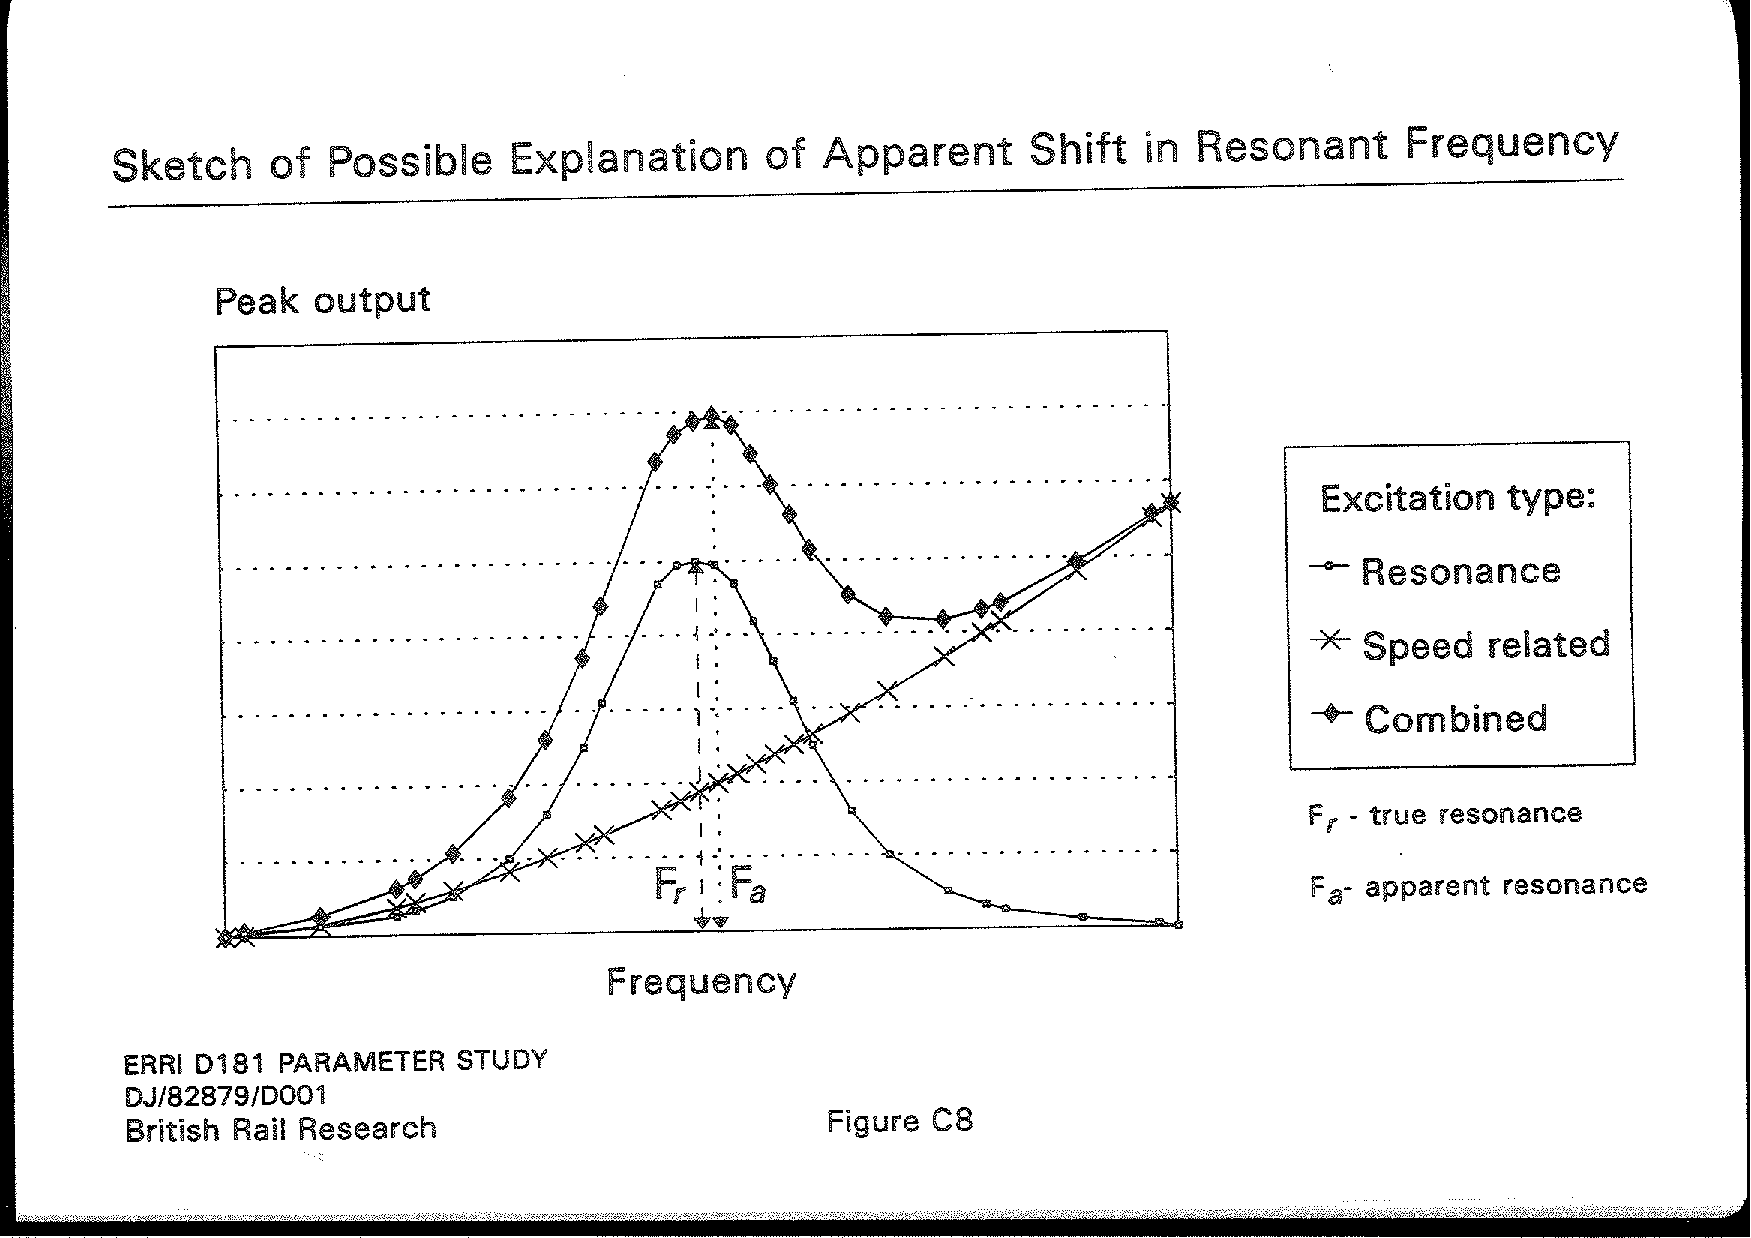
\includegraphics[width=\textwidth]{apparentshift}
    \caption{Sketch of Possible Explanation for Apparent Shift in Resonant Frequency. Extract from \citet[Appendix 2]{d181dt329}}
    \label{fig:apparentshift}
\end{figure}

In the sketch of possible explanation of apparent shift in resonant frequency(Figure \ref{fig:apparentshift}), the combined effect is the superposition of both resonance effect and speed-related effect. Speed-related effect simply increase when speed increase regardless of resonance. Speed is linear to frequency. Thus speed-related effect also simply increase when frequency increases. Resonance effect has an impact where frequency of train and bridge coincides. Speed-related effects is the cause for the frequency shift of combined peak output.

Both explanations indicate that apparent resonance frequency can hardly be predicted. Apparent frequency may even shift into domain lower than theory frequency. 


\section{Investigation of RP6}

\subsection{Debate on proposed 1.2Hz criterion}\label{sec:1.2criterion329}

The value of frequency limit, 1.2Hz is explained in \citet[p3.2: Criterion 2]{d181}:

\begin{quote}
To avoid the occurrence of resonance in the lateral motion of the vehicles due to the lateral motion of the bridge, a limit value lower than the first natural frequency $f_1t$ of the lateral vibration of the span studied should be fixed. The natural frequency for lateral movements is between 0.5 and 0.7 Hz for coaches and between 0.7 and 1 Hz for locomotives. We therefore propose a safety margin $F_{lt} \geq 1.2Hz$

\end{quote}

The original author of report RP6, mr.Graham Scott, was contacted to reveal the background of 'natural frequency for lateral movements'. Mr.Scott is still in charge of the development of software VAMPIRE and he's still active in the field. Unfortunately he was unable to remember what did 'natural frequency for lateral movements' stand for in previous quotes since it was written nearly 20 years ago. He passed me to his colleague Alan Minnis for further questions. Mr.Minnis stated following:

\begin{quote}
Looking at the values I think they would refer to typical rigid body modes of a vehicle.  These are independent of speed and a typical passenger coach with air suspension will have a lower sway frequency of around 0.6Hz which is within 0.5-0.7Hz.  Locomotives tend to have a slightly stiffer suspension hence the slightly higher frequency range.
\end{quote}

Mr.Minnis statements, combined with results yielded in supporting parametric report DT329 proves 1.2Hz criterion is aiming to avoid occurrence of resonance. But this isn't a feasible strategy for the following reasons:

\begin{enumerate} 
    \item The resonance between rigid body mode of train and first lateral vibration mode of the bridge has never been discussed in all D181 report series. No research proofed this kind of resonance can be critical in real life scenario.

    \item There are lots of evidence can be found in report DT329, showing resonance can happen on a bridge with a first lateral natural frequency even higher than 1.2Hz, which is self-conflicting with 1.2Hz criterion. In fact, the resonance could happen at any frequency on theory. However, the magnitude of resonance effect ranges from less pronounced to more pronounced from case to case.  

    For example, \citet[Page 14,Phase II]{d181dt329} shows resonance occurs on 1.71Hz:
        \begin{quote}
            The first lateral bending mode of this bridge is at 1. 71 Hz. The kinematic wavelength of the passenger coaches is around 34-38 m, giving a kinematic frequency range of 1.46 - 1.63Hz.Speeds of 58.14 m/s(1.53-1.71 Hz)and 64.6m/s(1.7-1.9Hz)were also done. The mid span lateral displacement for each of the time histories are shown in Figure C12(Orignial report). The slowest speed appears to show the greatest resonance.
        \end{quote}
\end{enumerate}

\subsection{Lateral forces on railway bridges}\label{sec:lateralforce329}

\subsubsection{Basic characteristics of lateral force on railway bridges}
It is concluded in initial phase of the study that presence of the bridge doesn't influence the track forces and track quality is a major factor in determining the lateral forces generated by a particular train on \citet[Page 7, Secondary Phase]{d181dt329}



\begin{quote}
    From the initial study [1], it was concluded that the track quality on a bridge is a major factor in determining the lateral forces generated by a particular train. The D181 Committee therefore asked BRR to determine the peak track forces generated over a wide range of track qualities.

    The length of a bridge is small compared to the overall length of a railway track and so track quality on a single bridge may not be representative of that on other bridges on the same route. However the initial study concluded that, in general, the lateral track forces are not influenced by the presence of the bridge.
\end{quote}

The resonance effects mentioned in the previous sections were only observed in deflection and acceleration domain due to the reason that the presence of the bridge doesn't influence the track forces. 


Influence on the total lateral force as a result of hunting of single vehicle bodies were examined. Three parameters were involved in this parametric research. They were vehicle speed, track irregularities deviation and wheel conicity.

Vehicle speed plays a key role. When speed is 60 km/h for freight trains, in the response output, there is very limited influence by increasing both track deviation and conicity. Different conicity tends to yield same force output. Same as track deviation. See Figure.\ref{fig:b1}.

\begin{figure}[h!]
    \centering
    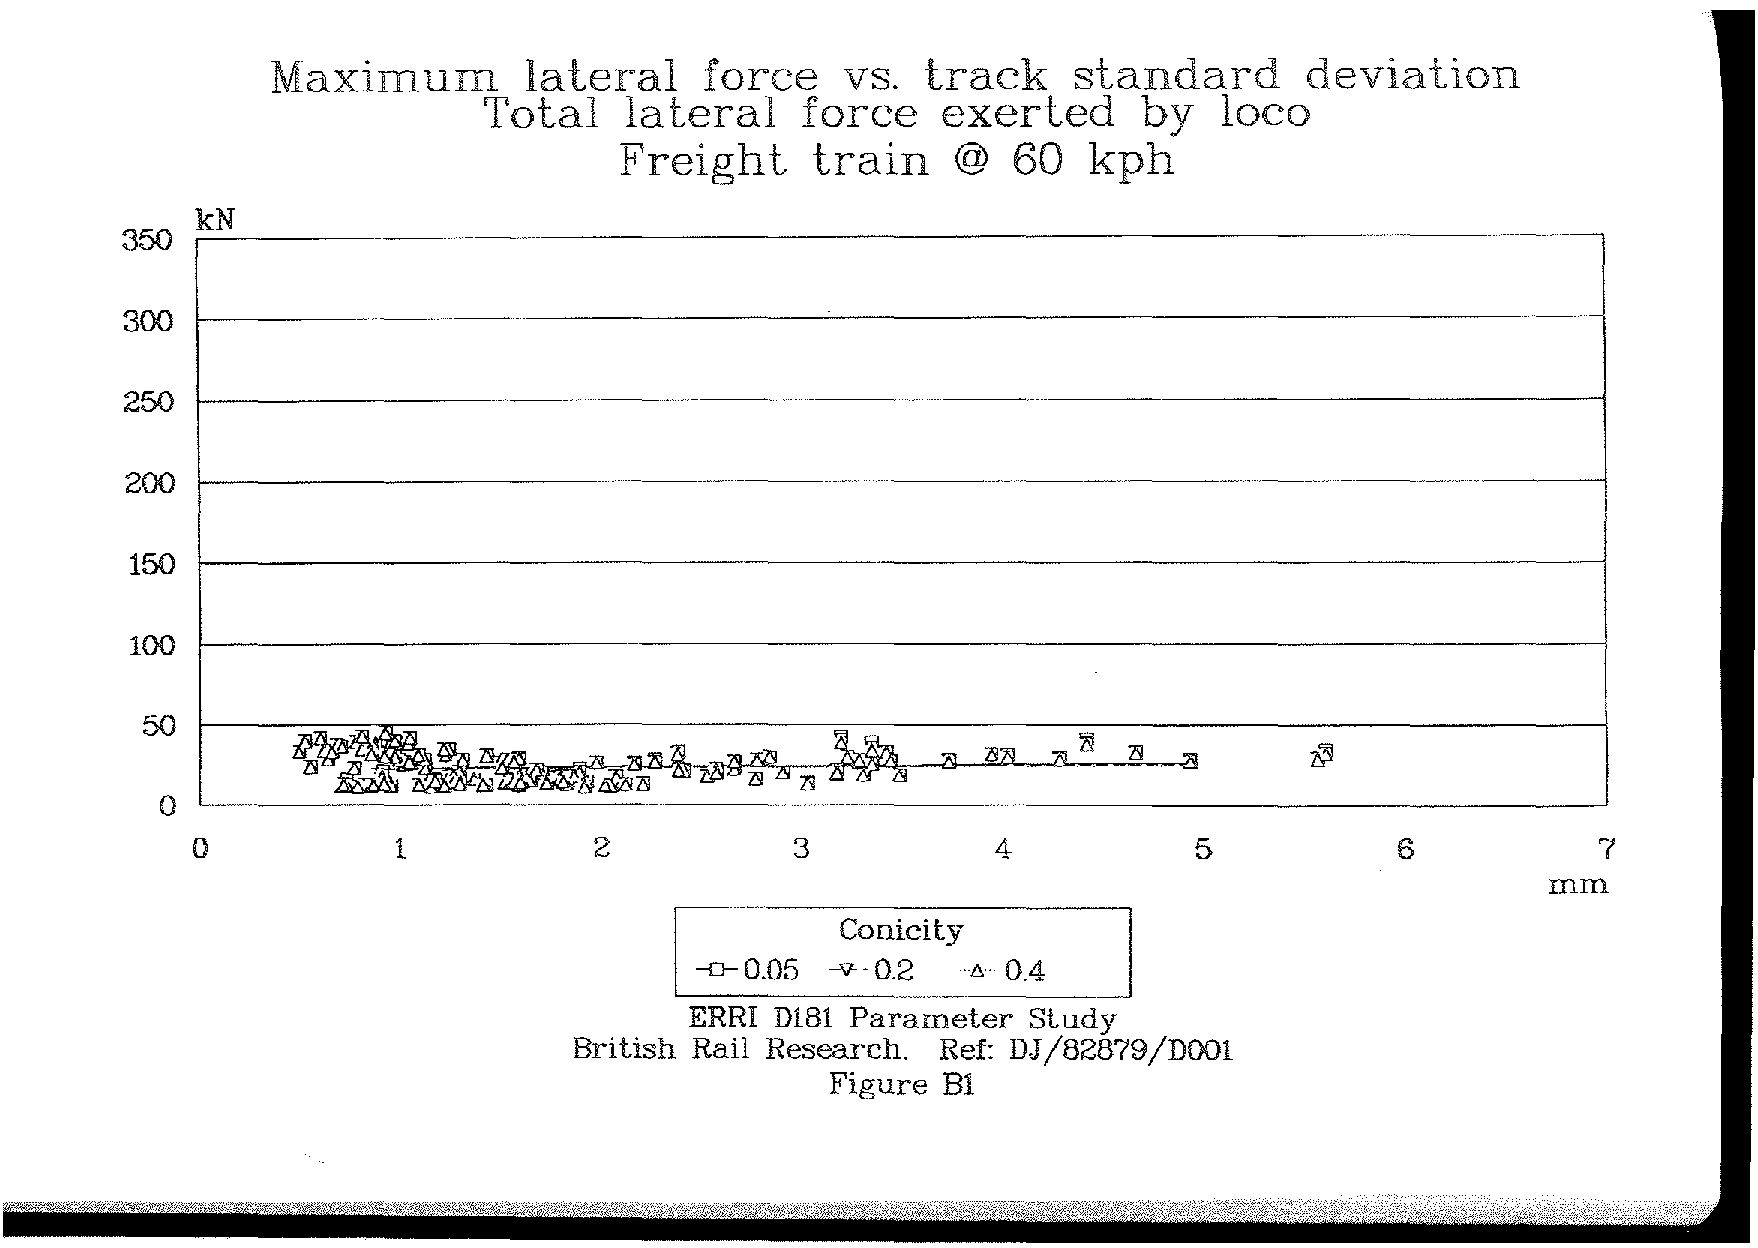
\includegraphics[width=0.8\textwidth]{b1}
    \caption{Figure B1 extracted from \citet{d181dt329}}
    \label{fig:b1}
\end{figure}


When speed increases, output of different conicity on same track deviation is more scattered. Similarly, increased deviation yields yields greater output. They are two basic trends observed in all output data.

However, it is uncertain which conicity will yield greater output compared to other 2 conicity setups. Surprisingly, in some cases, best maintained wheel profile (effective conicity 0.05) generates greater output than poorly maintained wheels (effective conicity 0.4). See Figure.\ref{fig:b2}. The most obvious case of this kind is freight train running at 100 km/h on track with 5.7mm (approximate) deviation.

\begin{figure}[h!]
    \centering
    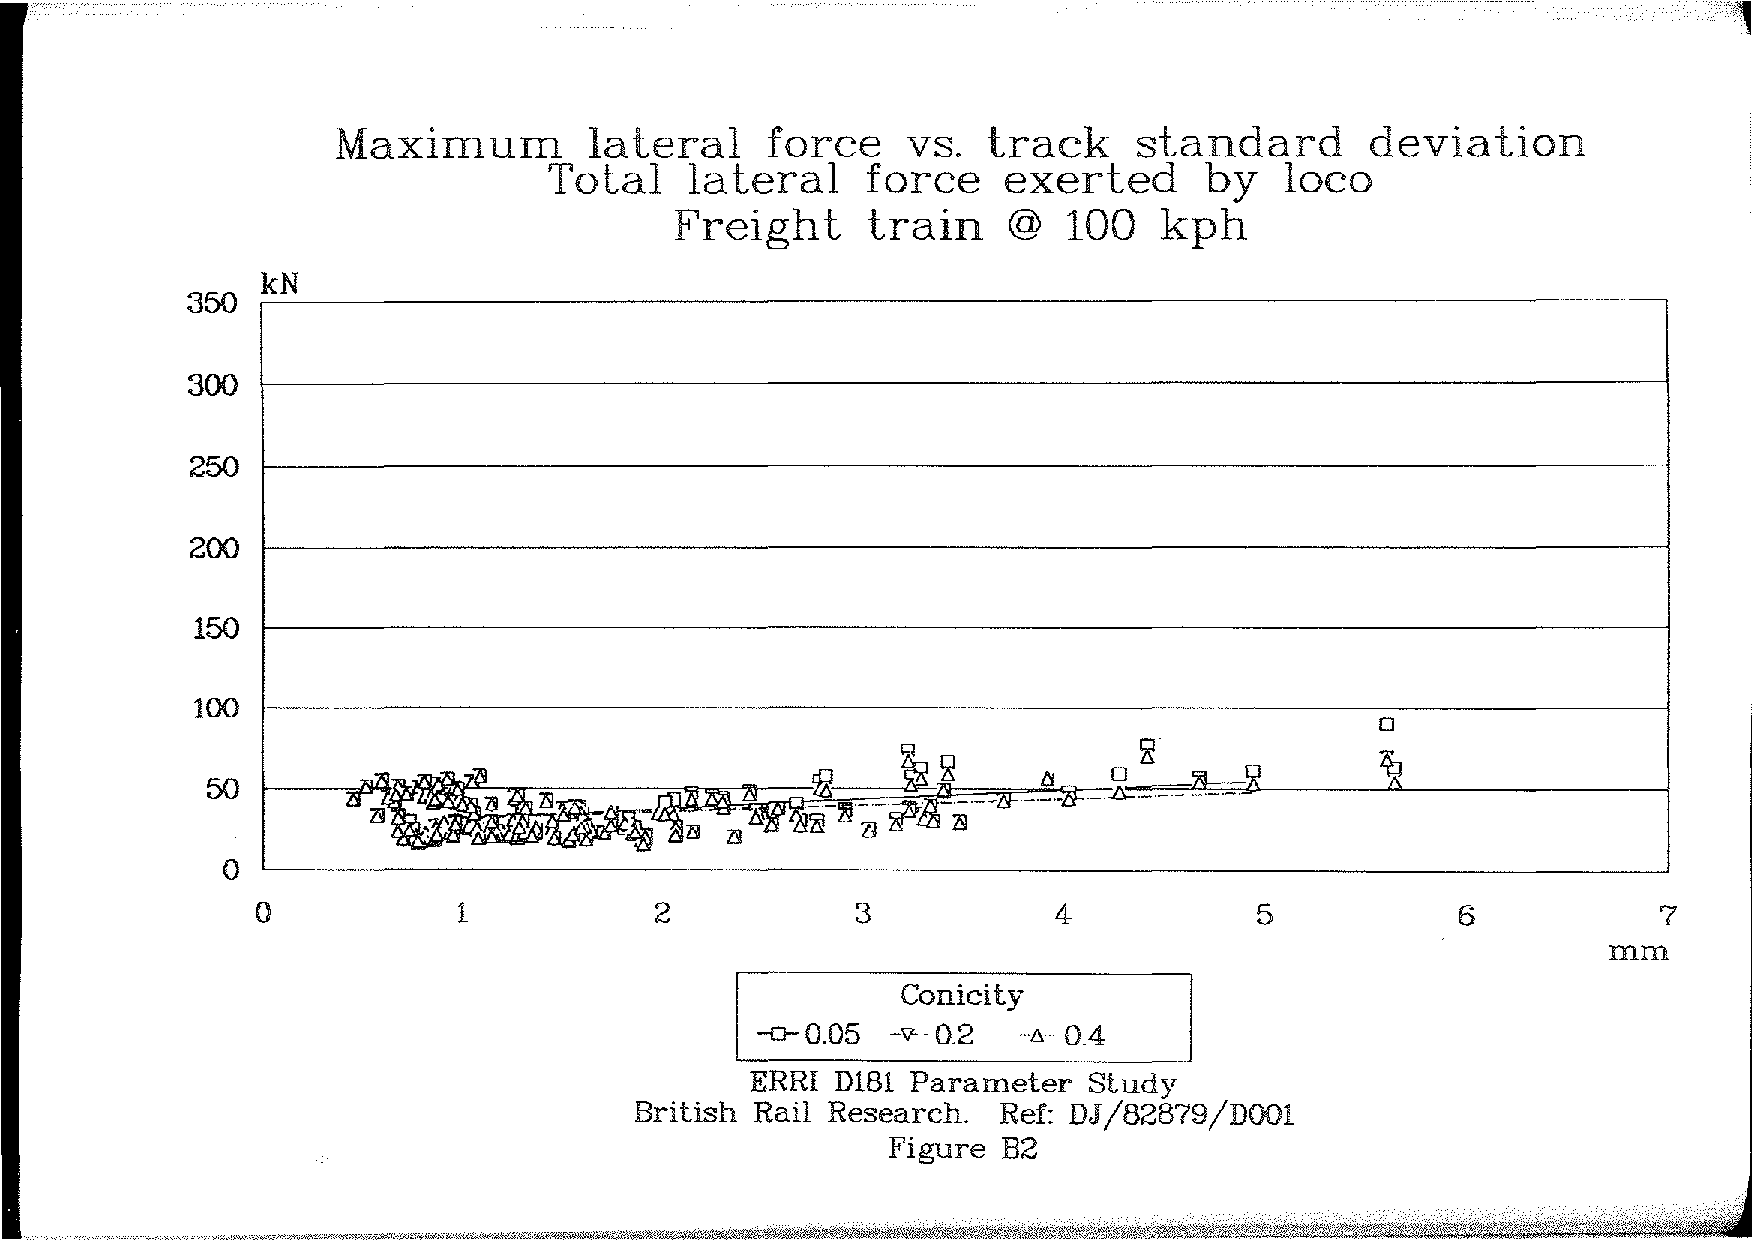
\includegraphics[width=0.8\textwidth]{b2}
    \caption{Figure B2 extracted from \citet{d181dt329}}
    \label{fig:b2}
\end{figure}

Different from conicity, the influence of increasing track deviation is simply predictable. Research report DT329 provided an approximate linear function for relationship between lateral force and track deviation. These linear functions can be extracted from plots B1-B30 of DT329.

Since peak force output of 120 km/h freight train and 200 km/h passenger train are close(2\% difference), it is reasonable to conclude that passenger train tends to yield smaller result than freight train at same speed. This is probably due to passenger trains have more sophisticated suspension system designed to suppress lateral motion of the vehicle. Unfortunately, only one speed of 200km/h configuration was available in DT329. But since freight train yields greater output, it is conservative for designer to adopt force output of freight trains for speeds of 60km/h, 100km/h, 120km/h.

It is worthy to point out a suspicious mistake of DT329 in Table.\ref{tab:peaklateralforce}. Report claimed that output data were filtered by statistical analysis. The peak lateral track force was determined from a statistical analysis of lateral track forces as $M \pm 3\sigma$ where $M$ is the mean lateral force value over the segment and $\sigma$ is the standard deviation over the segment. It does not give a true maximum lateral force but on which is greater than 99.5\% of all force values. It is obvious in Table.\ref{tab:peaklateralforce} that output data of 160kN for freight train wagon was not filtered by statistical analysis. It is the greatest value among all raw output data of freight train running at 100 km/h. See Figure.\ref{fig:b7}. This data of 160kN also illustrates that 
peak forces will be influenced by discrete features in the track geometry which may not be reflected thoroughly in the standard deviation. This thesis report suggest substitute 160kN with 80kN(value by approximate observation). See Table.[note1]\ref{tab:peaklateralforce}

\begin{figure}[h!]
    \centering
    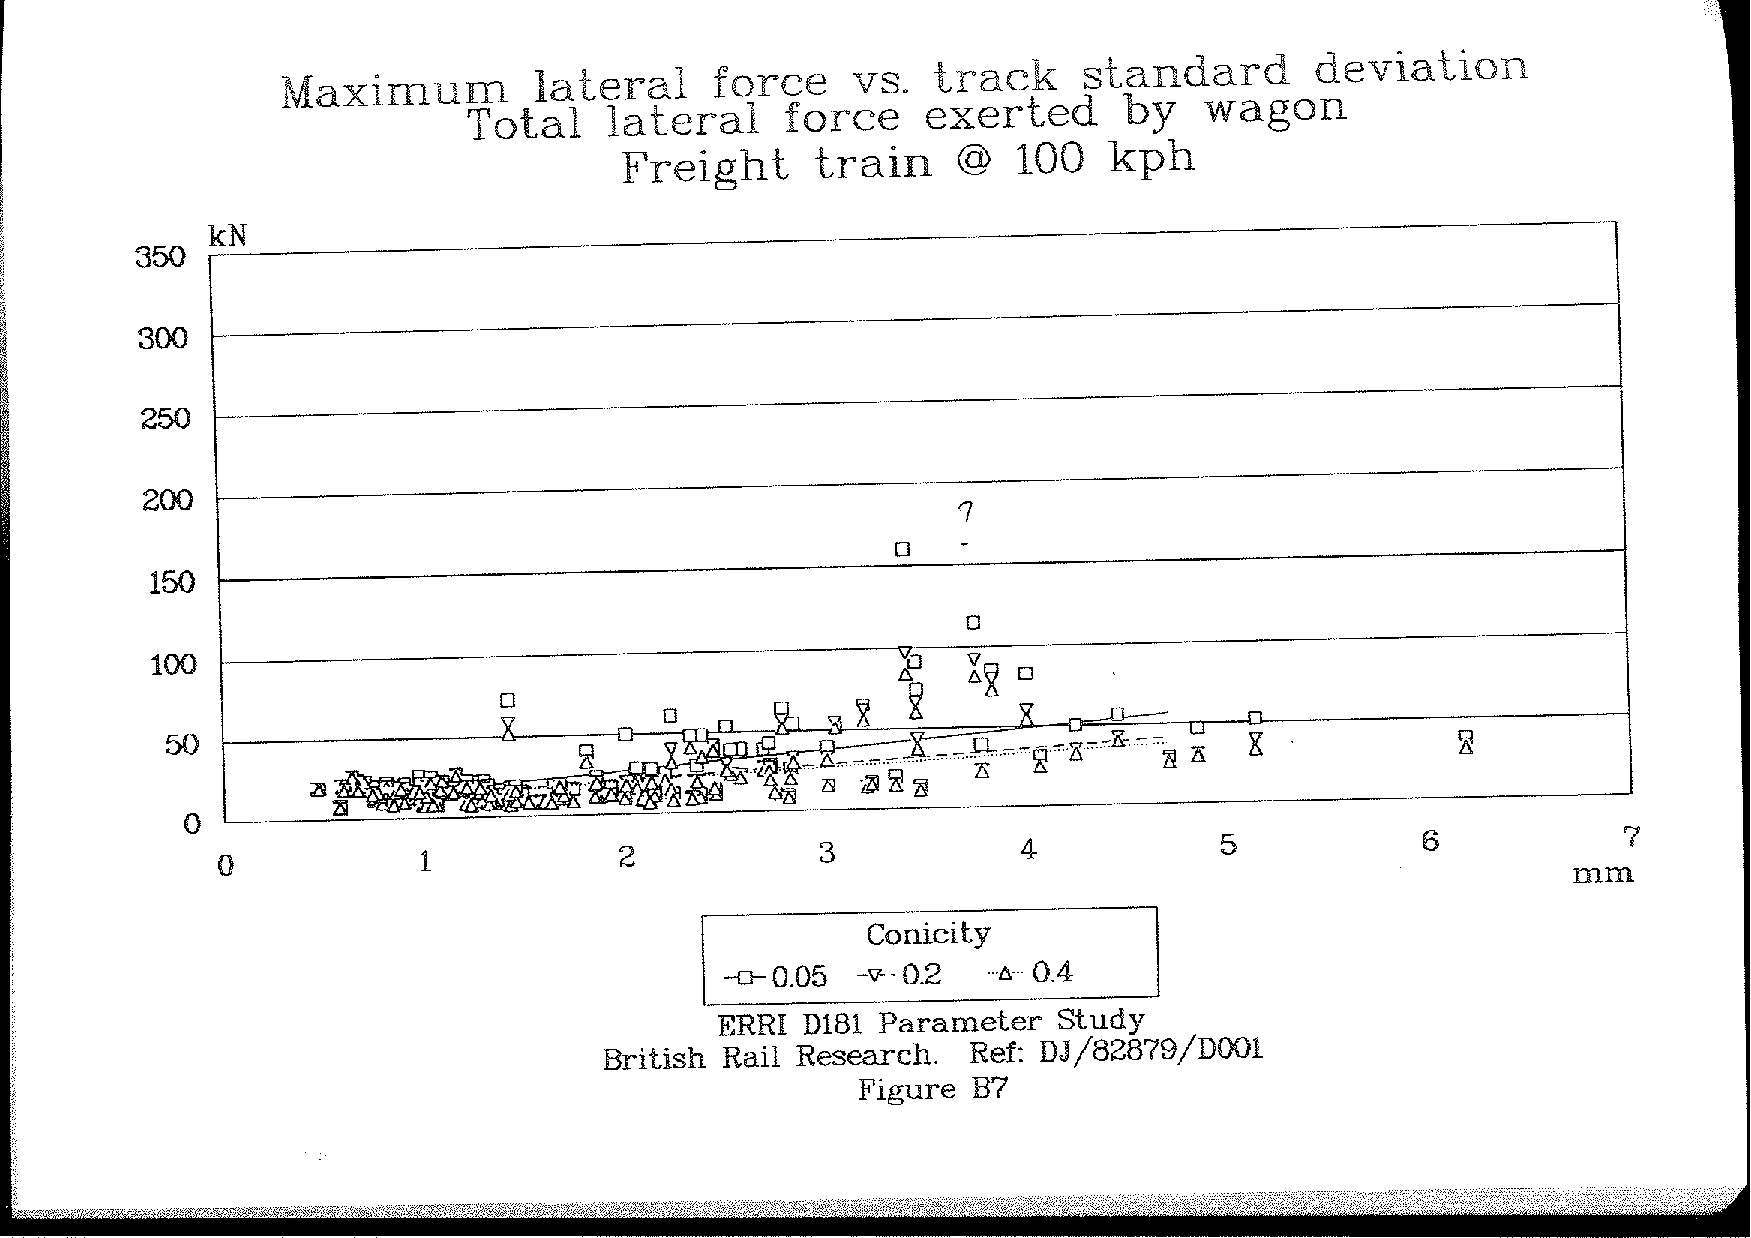
\includegraphics[width=0.8\textwidth]{b7}
    \caption{Figure B7 extracted from \citet{d181dt329}}
    \label{fig:b7}
\end{figure}

\begin{table}[h!]
    \centering
    \caption{Peak Lateral Track Force Over All Track Qualities. Extracted From \citet[Tab. B1]{d181dt329}}
    \begin{tabular}{cccc}
        \hline
        Peak lateral force(kN) & Locomotive Total & Coach/Wagon & Total \\ 
        \hline
        Freight 60 km/h & 50 & 60 & 110\\
        Freight 100 km/h & 90 & 160(\textbf{\textit{80}})$^1$ & 250(\textbf{\textit{170}})$^1$\\
        Freight 120 km/h & 75 & 110 & 185 \\
        Passenger 200 km/h & 140 & 50 & 190 \\
        High Speed 350 km/h & 125 & 125 & 250 \\
        Passenger 200 km/h(worn wheels) & 190 & 80 & 270 \\
        High Speed 350 km/h(worn wheels) & 330 & 225 & 555 \\
        \hline
    \end{tabular}
    \begin{flushleft}
    Note1: Force value 160kN for wagon of freight train running at 100 km/h is not representative. But it is not filtered by statistical analysis. It is advised to substitute 160kN with 80kN. 80kN is obtained by approximate observation of \citet[Figure B7]{d181dt329}. As a result, total force is reduced from 250kN to 170kN.
    \end{flushleft}
    \label{tab:peaklateralforce}
\end{table}

Speed and track quality are two most sensitive parameters. Control of track quality is more advisable compared to control of wheel conicity due to the reason that influence of track quality deviation is simply approximate linear to force output, whereas influence of wheel conicity has an unpredictable characteristic. Moreover, track quality can be controlled by using a maintenance regime.

\subsubsection{Refining of lateral force model}

Figure.\ref{fig:peaklateralforceregression} is created to plot total peak force illustrated in Table.\ref{tab:peaklateralforce}. 5 sets of data available were used to create the plot. 3 of them are data of freight train running at 60km/h, 100km/h and 120km/h. The other 2 sets of data are passenger train running at 200km/h and high speed train running at 350km/h respectively. Data produced with worn wheels profiles are neglected because they are not representative for normally maintained railway vehicles. Adjacent points were connected by solid lines. Different colour stands for different train types. Red lines and dots stand for freight trains. Blue stands for passenger trains and black stands for high speed trains. 

It is indicated that freight trains tends to have the biggest lateral force on track compared to other two kind of trains. And high speed train has lowest lateral force on track. This can be explained by freight trains possessing the most stiff suspension systems, while high speed trains possessing complicated suspension system to suppress lateral motion.

It can also be concluded that the relationship between lateral force and speed is not linear. As a general phenomenon observed, force increment decreases as speed increases. Regressions were made to better illustrate the trend of lateral force increment. Please note these regressions are only sufficient within the speed range plotted.

The first regression made was on freight train because it has the most sets of data. The form of function should satisfy:

\begin{enumerate}  
    \item 0kN lateral force when speed is 0km/h
    \item Simply increasing in value but generally decreasing in increment
\end{enumerate}

Finally function form $F=a*v^b$ is selected because its satisfying characteristics. R language was used to perform regression process. The regression result is also in good likelihood with original data. Achieved convergence tolerance was 2.868e-06. The result is presented in Formula.\ref{for:regressionfreight}. See Appendix.\ref{sec:Rregression} for code.

\begin{equation}
\label{for:regressionfreight}
F_{lf} = 5.2064\cdot v^{0.7495}
\end{equation}

Since 1 set of data is available for passenger train, Formula.\ref{for:regressionfreight} is scaled by a constant factor to create regression for passenger trains. Please note that this regression can not be verified because lack of data. However, since freight train has a greater lateral force then passenger train, it is conservative to adopt lateral force of freight train when calculating consequences related to passenger trains. It is still reasonable to adopt this regression since passenger trains are just simply less stiff than freight trains. 

Unfortunately, conducting such transient simulations is extremely time and resource consuming. It is impossible for this thesis to carry out more simulations to verify the sufficiency of following scaled regression. More data on passenger train and high speed train is recommended to be produced by future researches.

The scale factor $k_{pf}$ is obtained by comparing force value yielded by Formula.\ref{for:regressionfreight} at 200km/h and original passenger train force(190kN) data at 200km/h.

$$k_{pf} = \frac{190}{a_{lf}\cdot 200^{b_{lf}}}$$
$$a_{lp} = a_{lf}\cdot k_{pf}$$
merge above two equations, yield
$$a_{lp} = \frac{190}{200^{b_{lf}}} = \frac{190}{200^{0.7495}} \approx 3.58$$

and 

$$F_{lp} = a_{lp}\cdot v^{0.7495}$$

thus

\begin{equation}\label{for:regressionpassenger}
F_{lp} = 3.58\cdot v^{0.7495}
\end{equation}

Lateral force for high speed train were obtained in same manner. The scale factor $k_{hf}$ is obtained by comparing force value yielded by Formula.\ref{for:regressionfreight} at 350km/h and original high speed train force(250kN) data at 350km/h.

$$k_{hf} = \frac{250}{a_{lf}\cdot 350^{b_{lf}}}$$
$$a_{lh} = a_{lf}\cdot k_{hf}$$
merge above two equations, yield
$$a_{lh} = \frac{250}{350^{b_{lf}}} = \frac{250}{350^{0.7495}} \approx 3.10$$

and 

$$F_{lh} = a_{lh}\cdot v^{0.7495}$$
thus

\begin{equation}\label{for:regressionhighspeed}
F_{lh} = 3.10\cdot v^{0.7495}
\end{equation}


\begin{figure}[h]
    \centering
    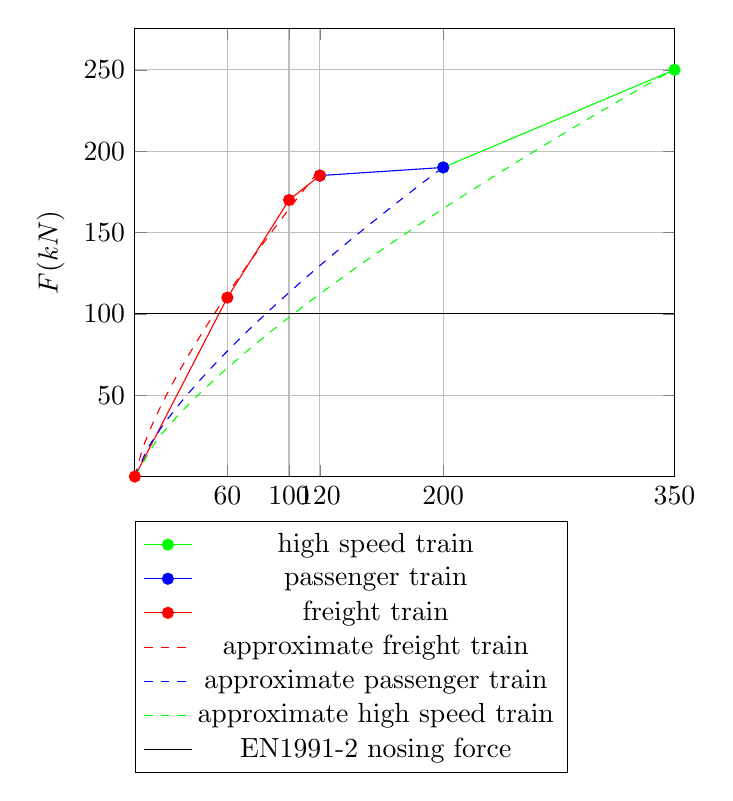
\begin{tikzpicture}
    \begin{axis}[
    % title = {Peak lateral track forces over all track qualities(worn profile scenario neglected)},
    xlabel={$v(km/s)$},
    ylabel={$F(kN)$},
    ymin = 0, xmin = 0, xmax = 350,
    grid = both,
    ytick = {50,100,...,250},
    xtick = {60,100,120,200,350},
    legend style={
    at={(0,0)},
    anchor=north west,at={(axis description cs:0,-0.1)}}] 
    ]
    \addplot[name path = C,mark=*, green] coordinates {(200,190) (350,250)};
    \addplot[blue,name path = B,mark=*] coordinates {(120,185) (200,190)};
    \addplot[red,name path = A,mark=*] coordinates {(0,0) (60,110) (100,170) (120,185)};
    \addplot[red,name path = D, domain = 0:120, dashed]{5.2064*x^0.7498};
    \addplot[blue,name path = E, domain = 0:200, dashed]{3.58*x^0.7498};
    \addplot[name path = F, domain = 0:350, dashed, green]{3.1*x^0.7498};
    \addplot[domain = 0:350] {100};
    \legend{high speed train, passenger train, freight train, approximate freight train ,approximate passenger train, approximate high speed train, EN1991-2 nosing force},
    \end{axis}
\end{tikzpicture}
\caption{Total peak lateral track forces over all track qualities(worn profile scenario neglected)}
\label{fig:peaklateralforceregression}
\end{figure}

\subsubsection{Application of lateral force model}
Formula\ref{for:regressionfreight},\ref{for:regressionpassenger} and \ref{for:regressionhighspeed} can be used as load forces for different design scenario. However, these loads are normally higher than the load defined in EN1991-2\citet[6.5.2 Nosing force]{EC12}. EN 1991-2 states that the characteristic value of the nosing force shall be taken as $Q_sk = 100 kN$. 

It is worthy to note that although in RP6\citet[Proposed criteria]{d181} several load model with loading magnitude ranging from 70 kN to 270 kN were originally proposed, EN1991-2 uses a single characteristic value of 100 kN for all design scenarios. 


Since no document has explained this modification, this is probably due to the consideration of lower track irregularity deviation during the creation of EN1991-2.

As explained in previous chapter, peak force is generally linear to track standard deviation. Most of the peak lateral force described in DT329 was obtained on track with 7mm standard deviation, while EN13848-5\citet{13848} allows much lower track standard deviation defined in Table \ref{tab:lateraldeviation}. This means peak lateral force on tracks(if maintained according to Eurocode regulations) is also much smaller than peak force obtained in DT329. 

EN1991-2 states the usage of nosing force. See \ref{sec:nosingforce}. Moreover, since loading model is obtained in Figure.\ref{fig:peaklateralforceregression}, a response solution of the bridge can also be obtained. 

This can be done by using the solution in \ref{sec:analyticalmodel} and substitute peak force into the formula as the amplitude of harmonic force $F$. Development of this method is presented in Chapter.\ref{sec:parcticalmethod}. 
 
It should be noted that the proposed model in RP6, as well as modified model in EN1991-2, is based on the investigation of first two traction units of the train. It is suspected that when bridge is longer, more traction units can run on the bridge simultaneously, introducing bigger force to the bridge. This can lead to a problem that EN1991-2 is non-conservative in the magnitude of nosing force when applied to longer bridges. However, this suspecting hypothesis is not verified in this chapter.  

\section{Evaluating nosing force proposed by EN1991-2}
The evualtation is done by comaparing peak result of calculation adopting nosing force and of FEM VAMPIRE simulation on the same bridge.

The bridge in Figure.\ref{fig:c9} is choosen with following parameters:

$l = 120m$

$Stiff: \sfrac{1}{10000}$  (defleciton/span ratio at midspan under 100kN point load at midspan )

$\mu = 6000kg/m$

Peak result for VAMPIRE simulation: 17mm

Accoridng to section.\ref{sec:nosingforce}, the characteristic value of the nosing force shall be taken as $Q_{sk} = 100kN$. It shall not be multiplied by the factor $\Phi$ or by the factor $f$. Thus, according to simple support Euler-beam theory, the deflection under 100kN nosing force is:

$\delta_{nosing} = 120m \cdot \sfrac{1}{10000} = 0.012m = 12mm$

It can be seen that nosing force doesn't give conservative result compared to VAMPIRE simulations. A resonance effect was reproduced in simulation. Thus the  reason for the nonconservative result is although some dynamic actions are taken into account by nosing force, the resonance effect is not included.


\section{Conclusion of D181 report series}
The report series managed to create load models for lateral dynamics railway effects. It is worthy to note that the lateral force on the track wasn't influenced by the presence of the bridge. The major influencing parameter for lateral force is track quality and conicity of the wheel profile. 

The resonance phenomenon was successfully reproduced and observed, though its only visible in deflection and acceleration domain. A basic characteristic of resonance, regardless of the type of resonance, is that apparent resonance frequency will shift from resonance frequency calculated on theory. The shift is unpredictable in the sense of both direction and magnitude. The effect related to speed start to creep in when speed is higher, making the effect of resonance less pronounced in higher speed(Figure \ref{fig:apparentshift}). 

Please note that every bridge will always have resonance with running train because axle repeat pattern and kinematic movement are both wavelength phenomenon, which means there is always a speed of train yielding a vibration frequency coincides with the first lateral natural frequency of bridge. However, the effect of resonance happening on long-span bridge is usually unpronounced since the speed of the train is low as 2.5m/s to 14m/s when resonance occurs.  

Some of the conclusion and proposed criteria in RP6 were adopted in Eurocode 1991-2. One of them is 1.2Hz criterion. It was adopted without amending. The other one is lateral force models. They were adopted in a different name as 'nosing force' in \citet[A6.5.2]{EC12}. 

The 1.2Hz criterion was under debate and proofed unreliable in fulfilling its original intention, avoiding occurrence of resonance. There is no research in D181 report series supporting this criterion, nor there exists literature behind the natural frequency of vehicles. This criterion ignored the fact that future bridge designs with long span would certainly have a natural frequency lower than 1.2 Hz. It is advised that Eurocode review this criterion and revise it.

Also, the nosing force proposed doesn't provide conservative result when there is resonance between the vehicle and the bridge.


% %!TEX root = main.tex


\chapter{Learning the lateral wavelength of Dutch railway vehicles by using the simulation results presented in D181 reports}\label{sec:wavelengthstudy}

As a conclusion in DT329 report, the lateral dynamic effects of railway vehicles are all wavelength phenomenon. The lateral wavelength of trains is a constant characteristics of themselves which doesn't change with outer environment. However, while the wavelength for axle repeat pattern is easy to get, the wavelength for kinematic movement normally requires heavy FEM simulations and post analysis of the response spectrum. 

Although it has been concluded in the previous chapter that avoiding resonance frequency is not a correct strategy for dynamics design in general, investigating the wavelength of trains can serve for the practical analysing methods that will be developed in following chapters in an alternative way.

This research aims to investigate both wavelength of trains running in the Netherlands. The axle repeat pattern wavelength is created by collecting all the possible axle layouts. The kinematic movement wavelength is created by developing a approximate methods that avoids heavy FEM simulations. 


\section{Effects investigated in wavelength study}

Effects investigated in this report will be the same effects investigated in DT 329, which is described in Sec.\ref{sec:resonance329}. However, according to the statement in Sec.2.3[Summary of results] in the same report,

\begin{quote}
Even when the axle repeat frequency matches the first lateral bending mode of each span, there is no evidence that the resonant behaviour of the span and train has any effect on subsequent spans, since the resonant effects do not appear to grow from span to span.
\end{quote}

the third investigated resonance effect 'coincidence between the length of the span and the kinematic wavelength of the trailing vehicles' is neglected in this thesis because it is concluded in \citet{d181dt329} that resonance do not grow from span to span. 


\section{Equivalent conicity used in this study}
According to \citet[Section.2.6]{esveld2001modern}, 

\begin{quote}
    Practical research has shown that over a period of time wheel profiles stabilise with wear at an equivalent conicity of 0.2 to 0.3. With regards to running stability, the equivalent conicity must remain below 0.4 and to ensure the centering effect it must be greater than 0.1.
\end{quote}

conicity range will be 0.2 to 0.3.

It is suggested by this report that vehicle maintenance sector ensure wheels of train wheels stay in the safe zone of conicity. 


\section{Study on wavelength of lateral kinematic movement}

The kinematic movememnt of the train on the rail is much similar to klingel movement. This section aims to assess the capability of using klingel formula to predict the wavelength of the whole train.

Klingel movement is proposed by Klingel which can well predict the moving trend of a single wheelset on a straight railway track. However, the kinematic movement of a certain wheelset assembled into a running train is different from the movement of a single free wheelset. This is due to multiple bodies interact with each other, introducing more complicated mechanism in wheel/rail interaction. 

This  study focuses on Klingel movement of a bogie. First part of the  study will try to discuss the relationship of Klingle frequency of a wheelset and kinematic movement frequency of a whole train. Second part of the study will use realistic data of Dutch railway/vehilces to assess the frequency bandwidth of Dutch native trains.

This section will include following parameters to be studied:

\begin{enumerate}[-]
	\item Speed of train, radius of the wheel and conicity of the wheel. 
	\item Gauge distance is fixed to 1435mm according to UIC standard. 
	\item Frequency is linear to speed if other parameters are fixed.
\end{enumerate}


\subsection{Comparison between Klingle movement and train kinematic movement studied in D181 DT329}

In this section the kinematic wave length of trains used in D181 VAMPIRE simulations will be calculated by klingel's formula and compared with the wavelength value obtained in VAPIRE simulation.

Klingel's formula:
Klingel has done experiments and has given that the wavelength of a single wheelset:

$$ \lambda_0 = 2 \pi \sqrt{\frac{rG}{2\gamma} }$$

where:

G = Dynamic Gauge

r = Dynamic Wheels Radius

g = Conicity

For 2 wheelsets connected by a bogie:

$$ \lambda = \lambda_0 \sqrt{1+(\frac{I}{G})^2}  $$

where:

I = Rigid wheel base

By inputting the related train parameters used in VAMPIRE simulations into the Klingel formula, following table is obtained.

\begin{table}[h]
  \centering
  \caption{Approxiamte letaral kinematic wavelength calcualted by improved Klingel formula}
    \begin{tabular}{cccccccccccccccc}
    \toprule
    & Gauge & BWD & Radius & Conicity & Wavelength($\lambda_0$) &Wavelength($\lambda$) & \\
    \midrule
    BR CLASS 56 LOCO  & 1435 & 4180 & 290 & 0.05 & 12.8175 & 39.4750 \\
    FS E444 LOCO  & 1435 & 2600 & 550 & 0.05 & 17.6517 & 36.5301 \\
    FS ETR500 LOCO  & 1435 & 3000 & 550 & 0.05 & 17.6517 & 40.9070\\
    UIC FREIGHT WAGON  & 1435 & 0 & 460 & 0.05 & 16.1430 & 16.1430 \\
    FS ETR500 COACH  & 1435 & 3000 & 440 & 0.05 & 15.7882 & 36.5883 & \\
    UIC COACH  & 1435 & 2560 & 445 & 0.05 & 15.8776 & 32.4718 &  \\
    \bottomrule
    \end{tabular}%
  \label{tab:wavelengthkinematic}%
\end{table}%


By comparing the result from Table.\ref{tab:wavelengthkinematic} and kinematic wavelength obtained by D181, extracted as Table.\ref{tab:329kinematicwavelength}, parametric study results show close prediction for kinematic wavelength of freight train locomotive/coach/wagon. It's because freight train suspension system is simpler and stiffer compared to passenger train's, making the behaviour of train acts more similar to the behaviour of a single wheelset of bigger mass. 


Wavelength for UIC freight wagon is a special case and it's not meeting the wavelength results in VAMPIRE simulations. This is probably because this car has a different design. It can be seen from in Figure.\ref{fig:uicoach} that only 2 axles are installed and there's no wagon installed. See Figure.\ref{fig:2axlefreight} and Figure.\ref{fig:4axlefreight} for their different axle configurations.

\begin{figure}[h]
	\centering
	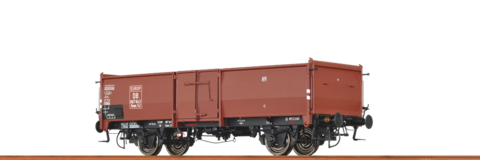
\includegraphics[width=0.5\textwidth]{2alxefreight.png}
	\caption{Example of a 2-axle freight wagon}
	\label{fig:2axlefreight}
\end{figure}

\begin{figure}[h]
	\centering
	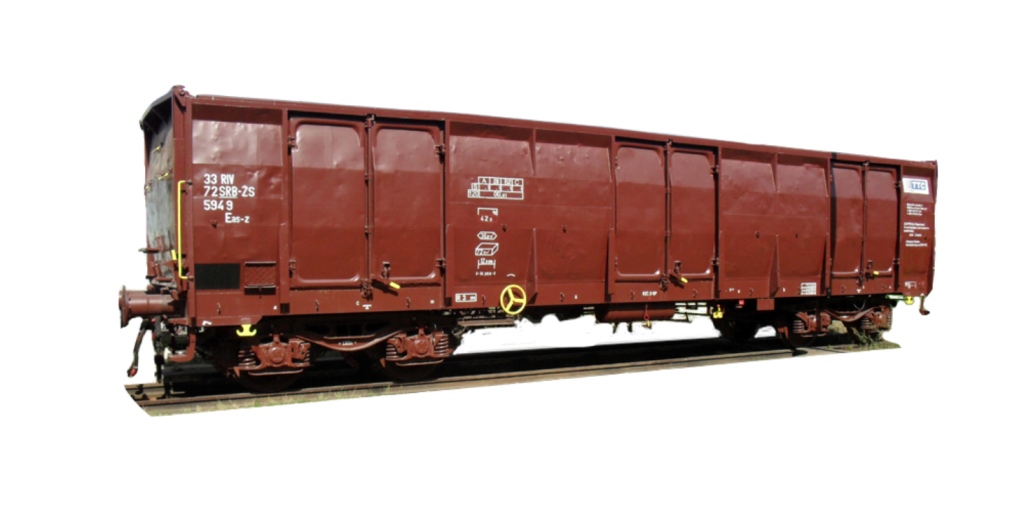
\includegraphics[width=0.5\textwidth]{4alxefreight.png}
	\caption{Example of a 4-axle freight wagon}
	\label{fig:4axlefreight}
\end{figure}


The train parameter used in this part of parametric study is attached in the Appendix.\ref{app:mu}. 


\section{Assess of wavelength bandwidth based on realistic data of Dutch Rail/Vehicle}

The wavelength of passenger coach is highly related to the characteristics of its suspension systems. These data are often difficult to obtain. Since the improved Klingel formula ignored the effect of suspension system, the results in this section is only approximate value for the wavelength of kinematic movement.


Future research is highly recommended to be conducted to study the kinematic wavelength of complete vehicles in the Netherlands, using realistic data of their suspension systems.


Table.\ref{tab:wavelengthrealistic} is created by processing Dutch wheel radius and wheelbase data collected from document\citet{trainparameters}. 
Thus range of $\lambda$ is obtained by inputting realistic data in Kingel formula, illustrated in Table.\ref{tab:wavelengthrealistic}.

\begin{table}[h]
  \centering
  \caption{Wavelength of kinematic movement generated by realistic value}
    \begin{tabular}{cccccccccccccccc}
    \toprule
    & Gauge & BWD & Radius & Conicity & Wavelength\_0() &Wavelength & \\
    \midrule
    \textbf{Freight 2-axle} & 1435 & 0 & 500 & 0.05 & 16.8303 & 16.8303 \\
    \textbf{} & 1435 & 0 & 500 & 0.2 & 8.4151 & 8.4151  \\
    \textbf{} & 1435 & 0 & 500 & 0.3 & 6.8709 & 6.8709  \\
    \textbf{}       &       &       &       &       &       &       &  \\
    \textbf{Freight 4-axle} & 1435 & 1800 & 500 & 0.05 & 16.8303 & 26.9988 \\
    \textbf{} & 1435 & 1800 & 500 & 0.2 & 8.4151 & 13.4994  \\
    \textbf{} & 1435 & 1800 & 500 & 0.3 & 6.8709 & 11.0222  \\
    \textbf{}       &       &       &       &       &       &       &  \\
    \textbf{Passenger} & 1435 & 2500 & 460 & 0.05 & 16.1430 & 32.4275 \\
    \textbf{} & 1435 & 2500 & 460 & 0.2 & 8.0715 & 16.2137  \\
    \textbf{} & 1435 & 2500 & 460 & 0.3 & 6.5904 & 13.2385 \\
    \textbf{}       &       &       &       &       &       &       &  \\
    \textbf{} & 1435 & 2750 & 460 & 0.05 & 16.1430 & 34.8947 \\
    \textbf{} & 1435 & 2750 & 460 & 0.2 & 8.0715 & 17.4473  \\
    \textbf{} & 1435 & 2750 & 460 & 0.3 & 6.5904 & 14.2457  \\
    \textbf{}       &       &       &       &       &       &       &  \\
    \textbf{Locomotive} & 1435 & 2400 & 500 & 0.05 & 16.8303 & 32.7960 \\
    \textbf{} & 1435 & 2400 & 500 & 0.2 & 8.4151 & 16.3980  \\
    \textbf{} & 1435 & 2400 & 500 & 0.3 & 6.8709 & 13.3889  \\
    \textbf{}       &       &       &       &       &       &       &  \\
    \textbf{} & 1435 & 2950 & 500 & 0.05 & 16.8303 & 38.4751 \\
    \textbf{} & 1435 & 2950 & 500 & 0.2 & 8.4151 & 19.2376  \\
    \textbf{} & 1435 & 2950 & 500 & 0.3 & 6.8709 & 15.7074  \\
    \bottomrule
    \end{tabular}%
  \label{tab:wavelengthrealistic}%
\end{table}%

For conservative usage, please take the value yielded by 0.3 wheel conicity. However, as proved in previous section, this estimation is in closest estimation of simulation results when concity is 0.05.

% Figure.\ref{fig:wavelengthkinematicfreight} and Figure.\ref{fig:wavelengthkinematicpass} are generated according to linear relationship between frequency and speed, using the wavelength $\lambda$ obtained in Table.\ref{tab:wavelengthrealistic}:

% $$ f = v \frac{1}{\lambda} $$


% \begin{figure}[h!]
% \centering
% \begin{tikzpicture}[trim axis left, trim axis right]
% \begin{axis}[
%     xlabel={$v(m/s)$},
%     ylabel={$f(Hz)$},
%     ymin = 0, xmin = 0, xmax = 44.4,
%     legend entries={$\sfrac{1}{\lambda}=0.059$,$\sfrac{1}{\lambda} =0.072$,$v=33.3 m/s$,$f=0.3Hz$},
%     grid = both,
%     minor y tick num= 4,
%     minor x tick num= 4,
%     legend pos = north west,
% ]
% \addplot[blue, domain = 0:44.4,samples=201,name path = A]{0.059*x};
% \addplot[red, domain = 0:44.4,samples=201, name path = B]{0.072*x};
% \addplot[mark=none, dashed]  coordinates {(33.3,0) (33.3,5) };
% \addplot[domain = 0:44.4,samples=10,dashed]{0.3};
% \addplot[gray] fill between[of=A and B];
% \end{axis}
% \end{tikzpicture}
% \caption{Lateral frequency of freight train with respect to speed(Kinematic movement)}
% \label{fig:wavelengthkinematicfreight}
% \end{figure}

% \begin{figure}[h!]
% \centering
% \begin{tikzpicture}[trim axis left, trim axis right]
% \begin{axis}[
%     xlabel={$v(m/s)$},
%     ylabel={$f(Hz)$},
%     ymin = 0, xmin = 0, xmax = 44.4,
%     legend entries={$\sfrac{1}{\lambda}=0.062$,$\sfrac{1}{\lambda}=0.076$,$v=33.3 m/s$,$f=0.3Hz$},
%     grid = both,
%     minor y tick num= 4,
%     minor x tick num= 4,
%     legend pos = north west,
% ]
% \addplot[blue, domain = 0:44.4,samples=201, name path = A]{0.062*x};
% \addplot[red, domain = 0:44.4,samples=201, name path = B]{0.076*x};
% \addplot[mark=none,dashed]  coordinates {(33.3,0) (33.3,3.5) };
% \addplot[domain = 0:44.4,samples=10,dashed]{0.3};
% \addplot[gray] fill between[of=A and B];
% \end{axis}
% \end{tikzpicture}
% \caption{Lateral frequency of passenger train with respect to speed(Kinematic movement)}
% \label{fig:wavelengthkinematicpass}
% \end{figure}

\section{Lateral wavelength of axle repeat pattern of Dutch Railway Vehicles}

This section will generate lateral wavelength value of axle repeat pattern of Dutch Railway Vehicles. Although DT329 provided wavelength values for some trains in Table.\ref{tab:329axlerepeat} but the way of obtaining these values was not mentioned. So an interpretation is needed to understand how to obtain the axle repeat pattern wavelength.

By observing Table.\ref{tab:329axlerepeat}, it can be seen that axle spacing layout is the only raw data needed to generate axle repeat pattern wavelength. The value is regardless of all other parameters. There are several axle space combinations in the table, but only one combination was finally put emphasis on during the analysis phase of axle repeat resonance research. They are

\begin{enumerate}[-]
    \item \textit{'wagon n axle m - wagon n+1 axle m'} for freight train, 
    \item \textit{'coach n axle m - coach n+1 axle m'} for passenger train,
    \item \textit{'coach n axle m - coach n+1 axle m'} for high speed train.
\end{enumerate}

It's still hard to comprehend above combinations so further interpretation is done by comparing it to train parameters in Appendix.\ref{app:dt329data}. It is found 

By comparing Fig.\ref{fig:trainparameters} and Table.\ref{tab:329axlerepeat}. It can be seen that 'wagon n axle m - wagon n+1 axle m' means the distance between one axle in the previous car and another axle in next car in the same location. The same goes for passenger train and high speed train. To better understand this spacing, please see L\_Coa in Figure.\ref{fig:trainparameters}. 

\begin{table}[h!]
  \centering
  \caption{Wavelength of axle repeat pattern($m$)}
    \begin{tabular}{rrrrrrrrr}
    \toprule
    \textbf{Type} & \textbf{L\_coa min} & \textbf{L\_coa max} & \textbf{2*L\_coa min } & \textbf{2*L\_coa max} \\
    \midrule
    \textbf{CB\_1} & 23.8  & 25.3  & 47.6  & 50.6 \\
    \textbf{CB\_2} & 25.3  & 27.5  & 50.6  & 55    \\
    \textbf{AB\_1} & 14.9  & 16    & 29.8  & 32     \\
    \textbf{AB\_2} & 18.8  & 19.5  & 37.6  & 39    \\
    \textbf{AB\_3} & 17    & 17.5  & 34    & 35   \\
    \textbf{AB\_4} & 18.7  & 19.2  & 37.4  & 38.4  \\
    \textbf{SA\_1} & 9.2   & 9.8   & 18.4  & 19.6  \\
    \textbf{SA\_2} & 12.8  & 13.5  & 25.6  & 27    \\

    \bottomrule
    \end{tabular}%
  \label{tab:wavelengthaxlerepeat}%
\end{table}%

Lateral wavelength of axle repeat pattern is then obtained by extracting all possible L\_Coa values from MU standards in \citet{EC15528}, illustrated in Table.\ref{tab:wavelengthaxlerepeat}. Detailed information about MU classes can be found in Appendix.\ref{app:mu}.


After examing the content in analysing section of DT329 resonance study, it is found that double length of L\_Coa is not taken into account in analysis phase. This means although D181 committee calculated double length of L\_Coa, these values were never used. Thus it is advisable for the usage of lateral axle repeat pattern wavelength, extracting only L\_Coa min column and L\_Coa max column.


% \begin{figure}[h!]
% \centering
% \begin{tikzpicture} 
%     \begin{axis}[
%     xlabel={$v(m/s)$},
%     ylabel={$f(Hz)$},
%     ymin = 0, xmin = 0, xmax = 44.4,
%     %legend entries={$i=0.057$,$i=0.07$,$v=33.3 m/s$,$f=0.3Hz$},
%     grid = both,
%     minor y tick num= 4,
%     minor x tick num= 4,
%     ]
%     \addplot[blue,name path=A,domain=0:44.4] {0.036*x};
%     \addplot[red, name path=B,domain=0:44.4] {0.042*x};
%     \addplot[black] fill between[of=A and B];
%     \addplot[blue,name path=C,domain=0:44.4] {0.051*x};
%     \addplot[red, name path=D,domain=0:44.4] {0.053*x};
%     \addplot[black] fill between[of=C and D];
%     \addplot[blue,name path=E,domain=0:44.4] {0.057*x};
%     \addplot[red, name path=F,domain=0:44.4] {0.059*x};
%     \addplot[black] fill between[of=E and F];
%     \addplot[blue,name path=G,domain=0:44.4] {0.063*x};
%     \addplot[red, name path=H,domain=0:44.4] {0.067*x};
%     \addplot[black] fill between[of=G and H];
%     \addplot[blue,name path=I,domain=0:44.4] {0.074*x};
%     \addplot[red, name path=J,domain=0:44.4] {0.078*x};
%     \addplot[black] fill between[of=I and J];
%     \addplot[blue,name path=K,domain=0:44.4] {0.102*x};
%     \addplot[red, name path=L,domain=0:44.4] {0.109*x};
%     \addplot[black] fill between[of=K and L];
%     \addplot[blue,name path=M,domain=0:44.4] {0.018*x};
%     \addplot[red, name path=N,domain=0:44.4] {0.021*x};
%     \addplot[gray] fill between[of=M and N];
%     \addplot[blue,name path=O,domain=0:44.4] {0.026*x};
%     \addplot[red, name path=P,domain=0:44.4] {0.027*x};
%     \addplot[gray] fill between[of=O and P];
%     \addplot[blue,name path=Q,domain=0:44.4] {0.029*x};
%     \addplot[red, name path=R,domain=0:44.4] {0.029*x};
%     \addplot[gray] fill between[of=Q and R];
%     \addplot[blue,name path=S,domain=0:44.4] {0.031*x};
%     \addplot[red, name path=T,domain=0:44.4] {0.034*x};
%     \addplot[gray] fill between[of=S and T];
%     \addplot[blue,name path=U,domain=0:44.4] {0.037*x};
%     \addplot[red, name path=V,domain=0:44.4] {0.039*x};
%     \addplot[gray] fill between[of=U and V];
%     \addplot[blue,name path=W,domain=0:44.4] {0.051*x};
%     \addplot[red, name path=X,domain=0:44.4] {0.054*x};
%     \addplot[gray] fill between[of=W and X];
%     \addplot[dashed,thick,red, domain=0:44.4] {0.3};
% \end{axis}
% \end{tikzpicture}
% \caption{Two repeat pattern frequencies with respect to speed}
% \label{fig:repeatpatternfrequencies}
% \end{figure}

\section{Conclusion of wavelength study}

The lateral resonance effects between running train and railway bridge include two phenomenon: Axle repeat pattern and Kinematic movement. Those two phenomenon are all wavelength phenomenon, which means for every specific train, the wavelength of its axle repeat pattern and kinematic movement remains constant. In other word, the frequency of lateral dynamic effect caused by the operating of trains on bridge is directly related to the speed.

Since the wavelength for the two phenomenon on the same train are not likely to be equal, the possible range of wavelength for both phenomenon were investigated in this chapter. The possible axle repeat pattern wavelength is approximately 10m-30m covering all train types and kinematic wavelength is 13m to 17m covering all train types. It can be seen that axle repeat pattern possess a broader range of wavelength than kinematic movement.

It also can be concluded that for any railway bridge, resonance between the bridge itself and train can happen if the train is running at a corresponding resonance speed according to its wavelength. So avoiding resonance is not a valid strategy to choose, not to mention the apparent frequency shift phenomenon to be discussed in Chapter.\ref{sec:resonance329}. 

To be noted that these wavelength are also not the exact wavelength in real-life scenario but an estimation, especially for kinematic movement. But it gave away a rough idea about the magnitude of trains' wavelength, and, can be used for practical design purposes. To see the usage of studied wavelength, please see Chapter.\ref{sec:parcticalmethod}.

\chapter{Development of new practical method for checking lateral resonance response of railway bridges based on VAMPIRE simulation results }\label{sec:parcticalmethod}

\section{Introduction}

This chapter proposes a new method for checking lateral resonance response of railway bridges. This method aims to provide an engineering solution for checking the deflection and acceleration of railway bridges when resonance happens under horizontal dynamic train load. Both creation and verification of the method is based on VAMPIRE simulation results provided in DT329 research.

The method features the combined usage of a simplified analytical structural model and a more refined lateral force model. The analytical structure model simulates a perfect resonance scenario for railway bridge. And the refined load model, which is a concentrated harmonic moving load, represents the lateral dynamic effects that occur because of the passing of the train. The combination of these two analytical elements will generate a resonance response conservative compared to the simulation output in DT329 because various types of disturbance were included in these simulation runs.

The analytical structural model that was introduced in Appendix.\ref{sec:analyticalmodel} and its explicit solution has already been worked out in the same chapter. Thus the main objective of this chapter is finding a better lateral force load model because current existing ones are too conservative(see Section.\ref{sec:refinedloadmodel}). The refined load model shall be able to be adopted universally for all regular train types. Once this load model is obtained and verified, it is then possible to take advantage of the combination of the load model and analytical solution for practical designing purposes.

\section{Overview of this chapter}

To give a clear overview of this chapter, procedure of development of the method  as following:

\begin{enumerate}
    \item \textit{Developing:} Develop a more practical load model to be used in pair with the analytical model introduced in previous chapter based on the VAMPIRE simulation outputs. See Section.\ref{sec:refinedloadmodel}
        \begin{enumerate}[label*=\arabic*.]
            \item Overview of both VAMPIRE numerical simulation method and analytical method. See Section.\ref{sec:overviewvampireanalytical}
            \item Find the analytical equivalent nosing forces amplitude for freight trains in 3 different cases presented in DT329 resonance research simulation. See Section.\ref{sec:findingequivalentamplitude}
            \item Find regular pattern and key parameter for the magnitude of nosing forces amplitude for freight trains. See Section.\ref{sec:keyparameterforequivalentamplitudeandhypothesis}
            \item Develop a conservative load model based on observed pattern of nosing force of freight trains. See Section.\ref{sec:keyparameterforequivalentamplitudeandhypothesis}
        \end{enumerate} 
    \item \textit{Verifying:} Validate the feasibility of combined usage of conservative load model and analytical model
        % \begin{enumerate}[label*=\arabic*.]
        %     \item What 
        % \end{enumerate}
    \item \textit{Finalizing:} Illustrate the usage of the method by applying it on a real railway bridge
\end{enumerate}

\begin{figure}[h!]
\centering
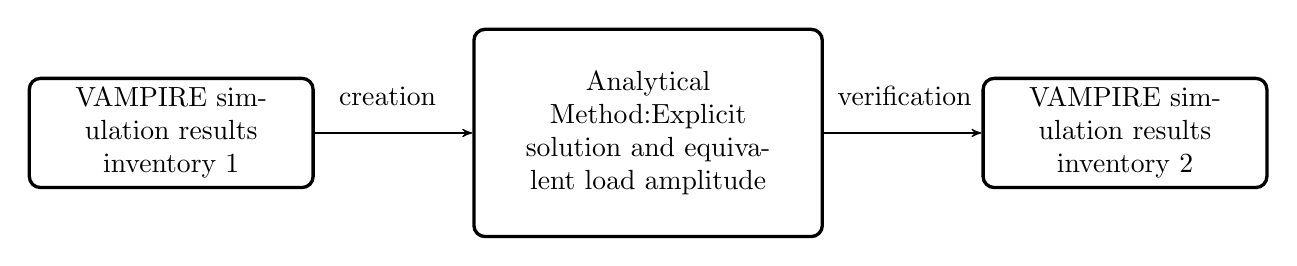
\begin{tikzpicture}[node distance=1cm, auto,]
    \node[punkt] (set1) {VAMPIRE simulation results inventory 1};
    \node[punkt, inner sep=15pt,right=2cm of set1]
        (am) {Analytical Method:Explicit solution and equivalent load amplitude};
    \node[punkt, right=2cm of am] (set2) {VAMPIRE simulation results inventory 2};
    \draw[->] (set1) to (am);
    \draw[->] (am) to (set2);
    \node[right=0.8cm of set1] (dummy1) {};
    \node[above=0.1cm of dummy1] (creation) {creation};
    \node[right=0.9cm of am] (dummy2) {};
    \node[above=0.1cm of dummy2] (verification) {verification};
\end{tikzpicture}
\caption{Workflow of the creation of analytical method}
\label{fig:workflowanalyticalmethod}
\end{figure}

\section{Development of refined load model}\label{sec:refinedloadmodel}

The load model provided in EN1991-2(nosing force) and D181 RP6(proposed criteria) are too conservative for dynamic analysis. The reason is that these forces are obtained by simulations ran on poorest maintained tracks with $7mm$ track irregularity standard deviation. In fact tracks are allowed to have lateral irregularities up to $1.8mm$ according to EN13848(Section.\ref{sec:lateraltrackirrgularities}). So existing lateral force models are enormous compared to real-life scenario. 

In addition, the existing load models are representative for hunting effects\citet[Proposed criteria]{d181}. However, according to \citet{majka2008effects}, although affected by varies parameters, critical speed for hunting effect is normally at 120km/h for modern railway vehicle and tracks. So at least for trains running slower than 120km/h, it can be conclude that hunting is not occurring. And their lateral force should be much less than the force magnitude mentioned in either EN1991-2 or D181 RP6.

Thus these existing load models are too big and not suitable for the analytical solution. A more precise load model is needed for coupled usage for analytical solution.

\subsection{Overview of VAMPIRE numerical simulation method and analytical method}\label{sec:overviewvampireanalytical}

The analytical model itself and its explicit expression have already been introduced and described in previous chapter. This section will give a overview on the input parameters of both VAMPIRE simulation and analytical model. This is not only due to the fact that VAMPIRE simulation was proved by D181 committee to be in close prediction with situ measurements, but also because in following sections VAMPIRE simulation results will be used as benchmark data for the development of analytical model's pairing load model. 

\begin{table}[h!]
    \centering
    \caption{Comparison between input parameters of DT329 VAMPIRE simulations and analytical model}
    \begin{tabular}{c|cc}
        \hline
        & Simulation & Analytical model \\
        \hline
        Bridge structure & simply supported beam & simply supported beam \\
        Span & Yes & Yes \\
        Stiffness & Yes & Yes \\
        Mass & Yes & Yes \\
        Damping & Yes & Yes \\
        Train & complete train as mass spring system & single moving harmonic load \\
        Train Speed & Yes & Yes \\
        Track irregularities & Yes & No \\
        Wheel profile & Yes & No \\
        Wheel-rail interaction & Yes & No \\
        \hline
    \end{tabular}
    \label{tab:comparisonsimulationanalytical}
\end{table}

As demonstrated in Table.\ref{tab:comparisonsimulationanalytical}, while input parameters for simulation are complicated, analytical model possesses less input parameters. 

That table shows that the single moving harmonic load in analytical model shall be capable of providing dynamic effect caused by train speed, track irregularities, wheel profile and wheel-rail interaction to the analytical model. Correct single moving harmonic load input shall yield the same result as VAMPIRE simulation provided that same span, stiffness, mass and damping value are adopted in both two calculating methods.

Thus finding the correct expression for the harmonic moving force is vital to the analytical model. The harmonic moving force has 3 parameters: speed $c$, frequency $\Omega$  and amplitude $Q$. Since speed $c$ simply equals to train speed and frequency $\Omega$ equals to the first natural bending frequency of the beam $\omega_1$, the amplitude of the harmonic force remains to be researched. Further development of the amplitude expression will be discussed in following sections.



\subsection{Finding equivalent lateral force amplitude for specific cases}\label{sec:findingequivalentamplitude}
In this section, equivalent lateral force amplitudes for the analytical solution are obtained. The equivalent lateral force amplitude does not represent real force magnitude in rail/wheel interaction, but a force amplitude that yields same result as VAMPIRE simulations using same input parameters if substituted into analytical solution. So this lateral force amplitude may not be correct if adopted in other structure models. On the other hand, analytical solution may yield imprecise results if not substituted with this exact equivalent force amplitude. They can only be used in pair with each other.

Thus in order to perform the comparison mentioned above, both input and output data of DT 329 VAMPIRE simulations are selected as reference data. The input data will be substituted into analytical model and the output data of VAMPIRE simulation will be compared with output of analytical model. 

3 sets of reference data are extracted from DT329 report. They are C1,C3,C9 in Figure.\ref{fig:c1},\ref{fig:c3} and \ref{fig:c9} respectively. These data are all extracted from resonance study so they are qualified to be used as reference data. Please note that C1,C3,C9 were all done on freight trains on same track sample. Finally 3 equivalent forces are collected from these 3 test samples to see regular pattern and relevant parameters for freight trains.

\begin{figure}[h!]
    \centering
    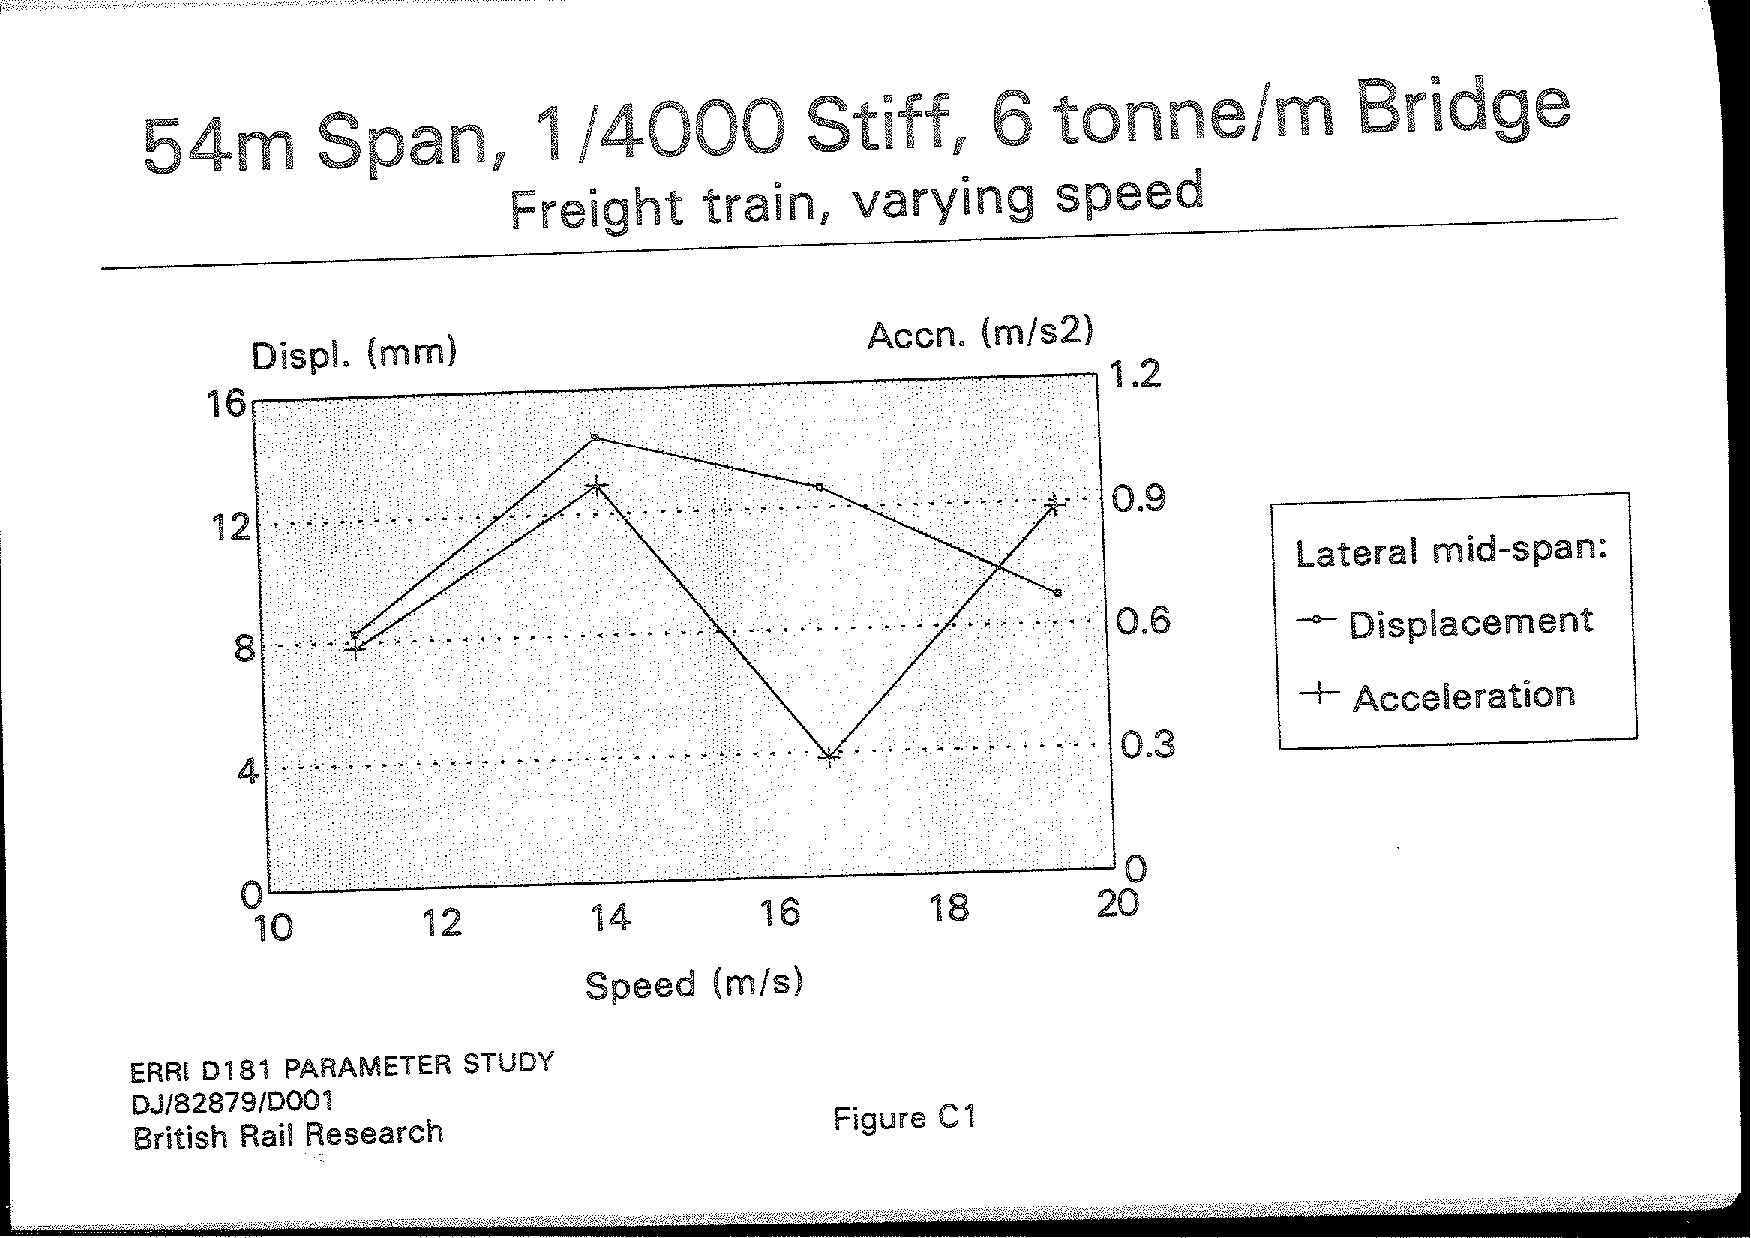
\includegraphics[width=0.8\textwidth]{c1}
    \caption{Figure C1 extracted from \citet{d181dt329} }
    \label{fig:c1}
\end{figure}

\begin{figure}[h!]
    \centering
    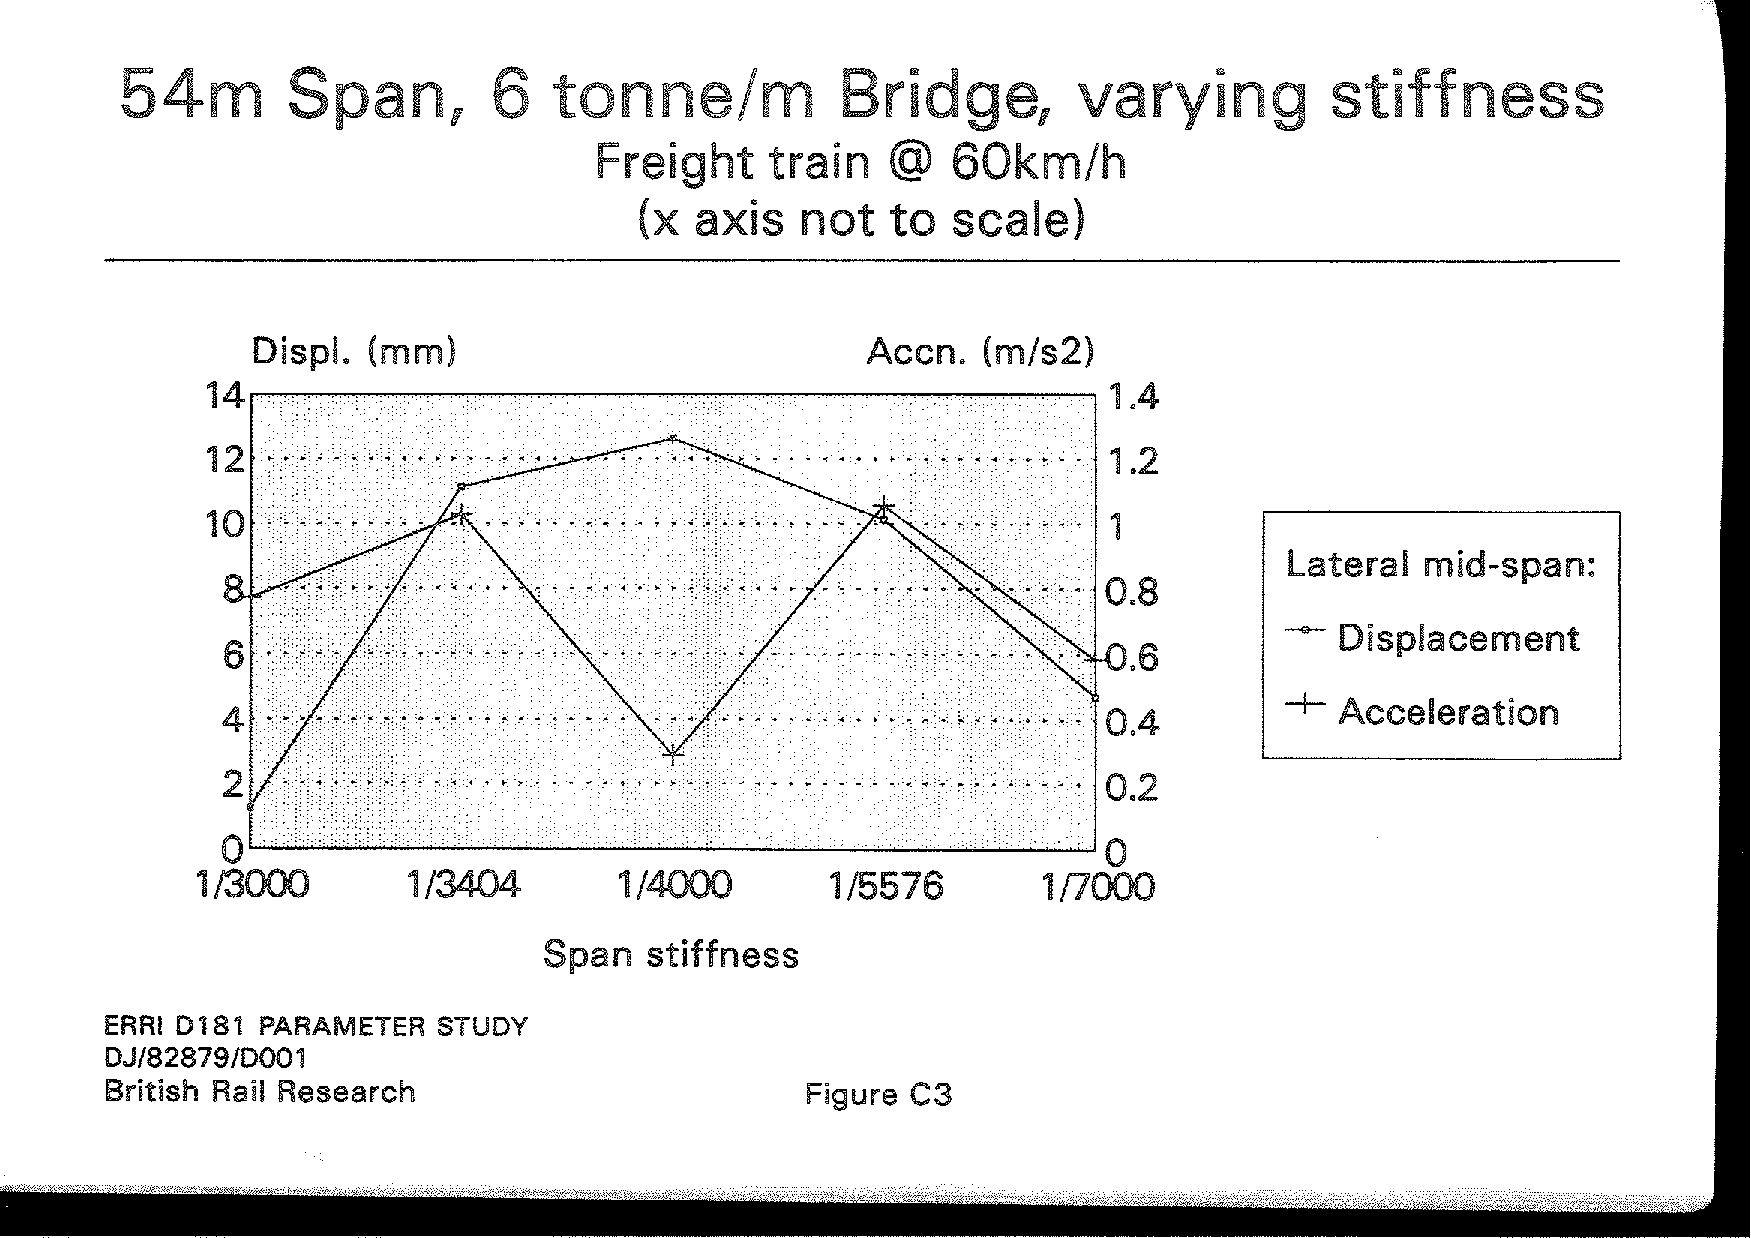
\includegraphics[width=0.8\textwidth]{c3}
    \caption{Figure C3 extracted from \citet{d181dt329} }
    \label{fig:c3}
\end{figure}

\begin{figure}[h!]
    \centering
    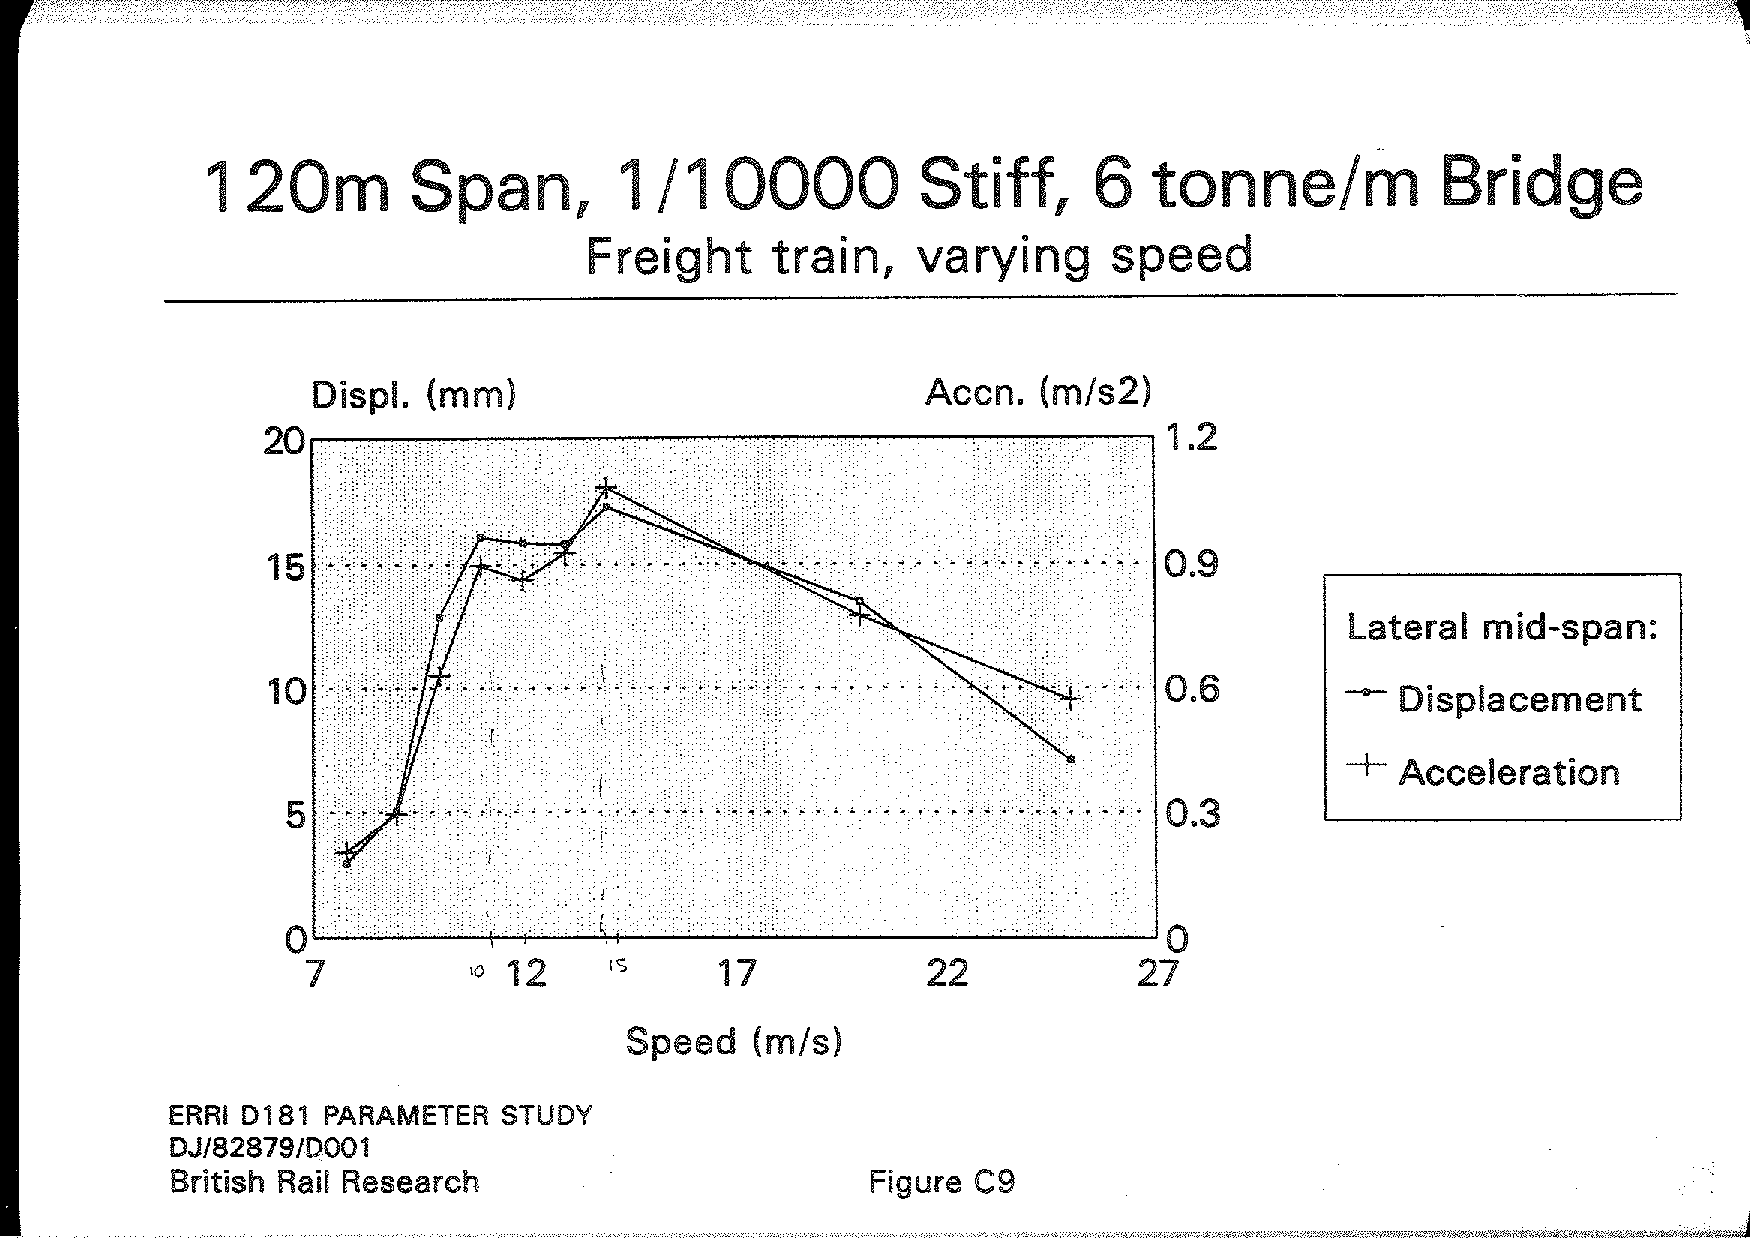
\includegraphics[width=0.8\textwidth]{c9}
    \caption{Figure C9 extracted from \citet{d181dt329} }
    \label{fig:c9}
\end{figure}

By observing Eq.\ref{eq:v(x,t)simpleharmonic}, it is concluded that force amplitude is an independent variable and perfectly linear to the analytical output. Thus the equivalent force is obtained by inputing bridge parameters and train speed into the analytical solution Eq.\ref{eq:v(x,t)simpleharmonic} and manually increasing the force amplitude little by little until the peak response output reaches the same magnitude of peak simulation output. The parameters used and their corresponding results are presented in Table.\ref{tab:parametersetupsandequivalentforce}.


\begin{table}[h!]
    \centering
    \caption{Parameter setups and equivalent force amplitude for C1,C3,C9}
    \begin{tabular}{c|ccc}
        \hline
        & C1 & C3 & C9 \\
        \hline
        Stiffness($\sfrac{\delta_0}{l}$) & 1/4000 & 1/4000 & 1/10000 \\
        Span($m$) & 54m & 54 & 120 \\ 
        Mass per unit length($kg/m$) & 6000 & 6000 & 6000\\
        Speed of train($m/s$) & 14 & 16.67(60km/h) & 14\\
        Damping ratio & 1\% & 1\% & 1\%\\
        Train type & Freight & Freight & Freight \\
        Track & Coupled freight track & Coupled freight track & Coupled freight track \\
        \hline
        Equivalent load amplitude(kN) & 14 & 15 & 14 \\
        \hline
    \end{tabular}
    \label{tab:parametersetupsandequivalentforce}
\end{table}

\subsection{Key parameter for equivalent force amplitude and hypothesis expression for refined load model}\label{sec:keyparameterforequivalentamplitudeandhypothesis}

By observing the equivalent load amplitude illustrated in Table.\ref{tab:parametersetupsandequivalentforce}, it is found that the equivalent load amplitude yielded by analytical solution meets the general principle of lateral track force concluded by DT329 track quality research. The general principle is that the lateral force is only relevant to speed if track quality and wheel conicity are fixed. And lateral force is irrelevant to the bridge parameters.
 
Because equivalent force amplitude meets the general lateral force principle, it is further expected that the equivalent force amplitude also has a similar form of force-speed relationship of DT329 VAMPIRE simulations. Due to the lack of reference data, it is impossible to make a reliable regression. Only a hypothesis expression can be created by scaling Eq.\ref{for:regressionfreight} to 14kN at 14m/s(reference data set C1). Please note only C1 was used in creating the hypothesis expression so C3 and C9 remains available for the verification.

\begin{equation}
    Q= 1928\times c^{0.7495}
\end{equation}

where:

$Q$: equivalent force amplitude($N$)

$c$: speed of the train($m/s$)

This scaling is reasonable because: according to the conclusion of DT329 track quality research, lateral forces generated on 7mm standard deviation tracks has a certain relationship with speed(Eq.\ref{for:regressionfreight}). And it is also concluded that at same speed, lateral forces are linear to the track stand deviation. Thus, since all 3 reference data are run on the same track, force output of analytical model at each speed(14m/s and 16.67m/s) could be scaled from Eq.\ref{for:regressionfreight} 's results at these speeds. Furthermore, a scale factor is then applied on Eq.\ref{for:regressionfreight} to reflect the scaling to the whole speed domain and this yields above equation.

As a conclusion, this hypothesis expression is obtained by processing the output of VAMPIRE simulation on freight trains and coupled freight track(poorer than passenger line and high speed line). So it is in closest prediction in the effects generated by freight trains. However, since passenger trains and high speed trains yields lower lateral force compared with freight trains, this hypothesis expression remains conservative for all train types.

\section{Verification of the method}

In this section the combined usage of analytical model and hypothesis expression for equivalent force amplitude is examined and verified. A matlab script is written to function the analytical model with hypothesis expression for equivalent load amplitude implemented. Now that force amplitude $Q$ is a function of speed, it's no longer necessary to input the force amplitude manually. To verify the correctness of combined usage of these two elements, other reference data from resonance research in DT329 are selected and presented in Figure.\ref{fig:c12}, \ref{fig:c13} and \ref{fig:c14}. 

\begin{figure}[h!]
    \centering
    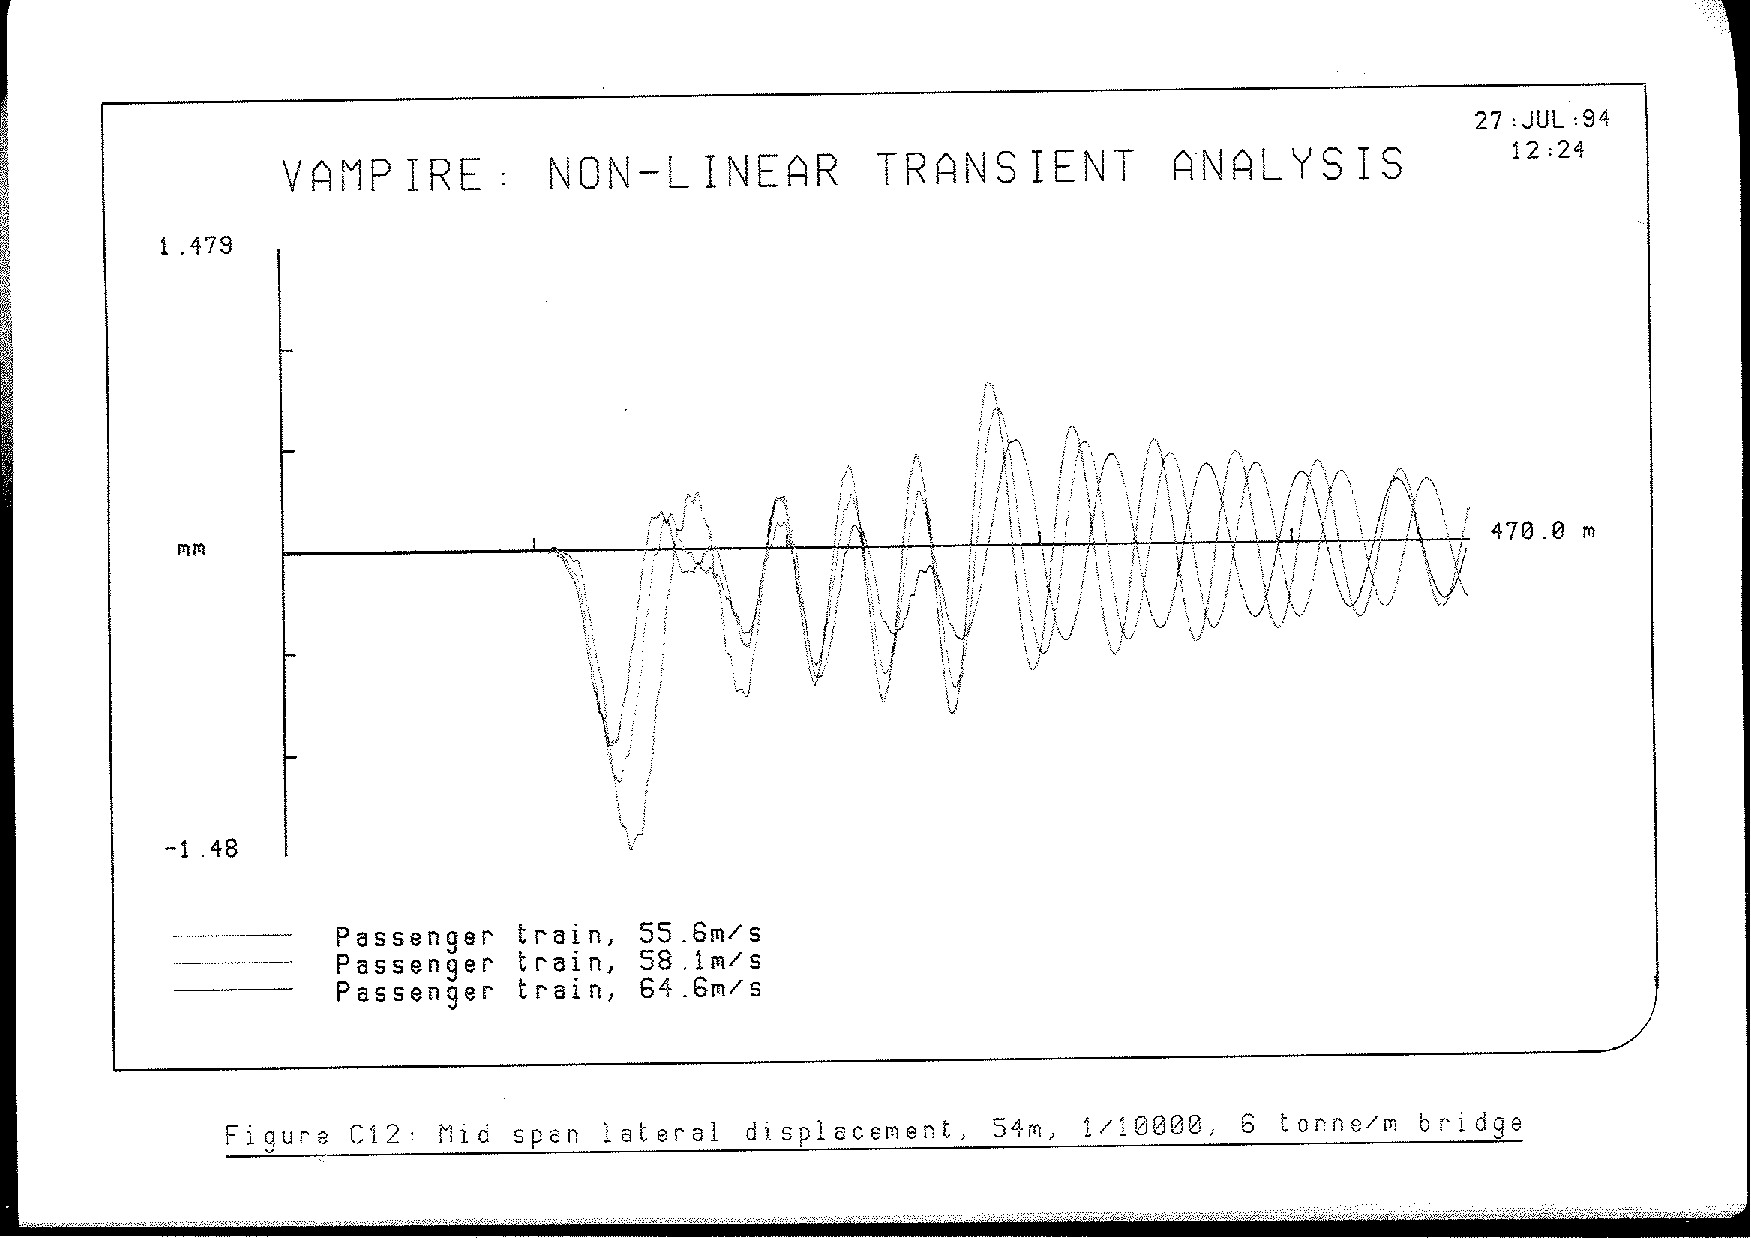
\includegraphics[width=0.8\textwidth]{c12}
    \caption{Figure C12 extracted from \citet{d181dt329} }
    \label{fig:c12}
\end{figure}

\begin{figure}[h!]
    \centering
    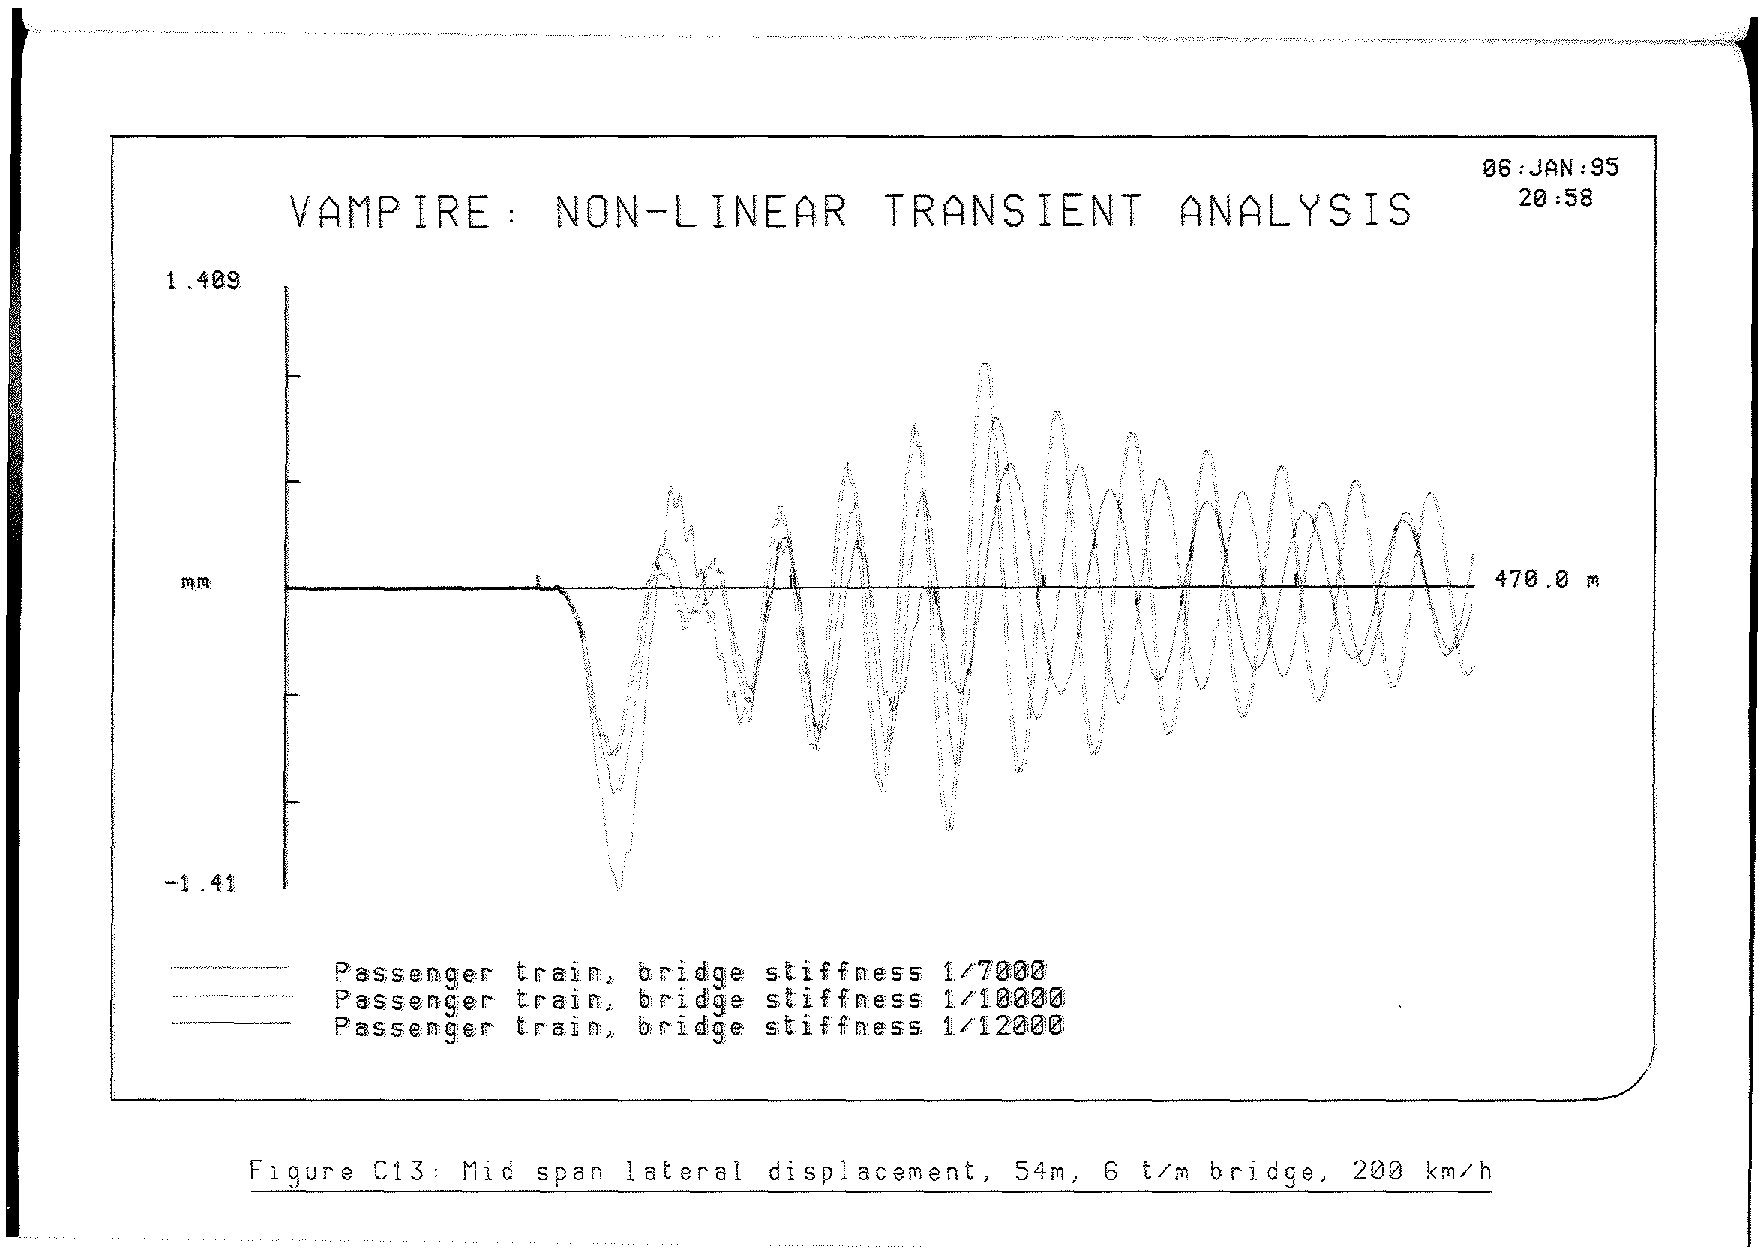
\includegraphics[width=0.8\textwidth]{c13}
    \caption{Figure C13 extracted from \citet{d181dt329} }
    \label{fig:c13}
\end{figure}

\begin{figure}[h!]
    \centering
    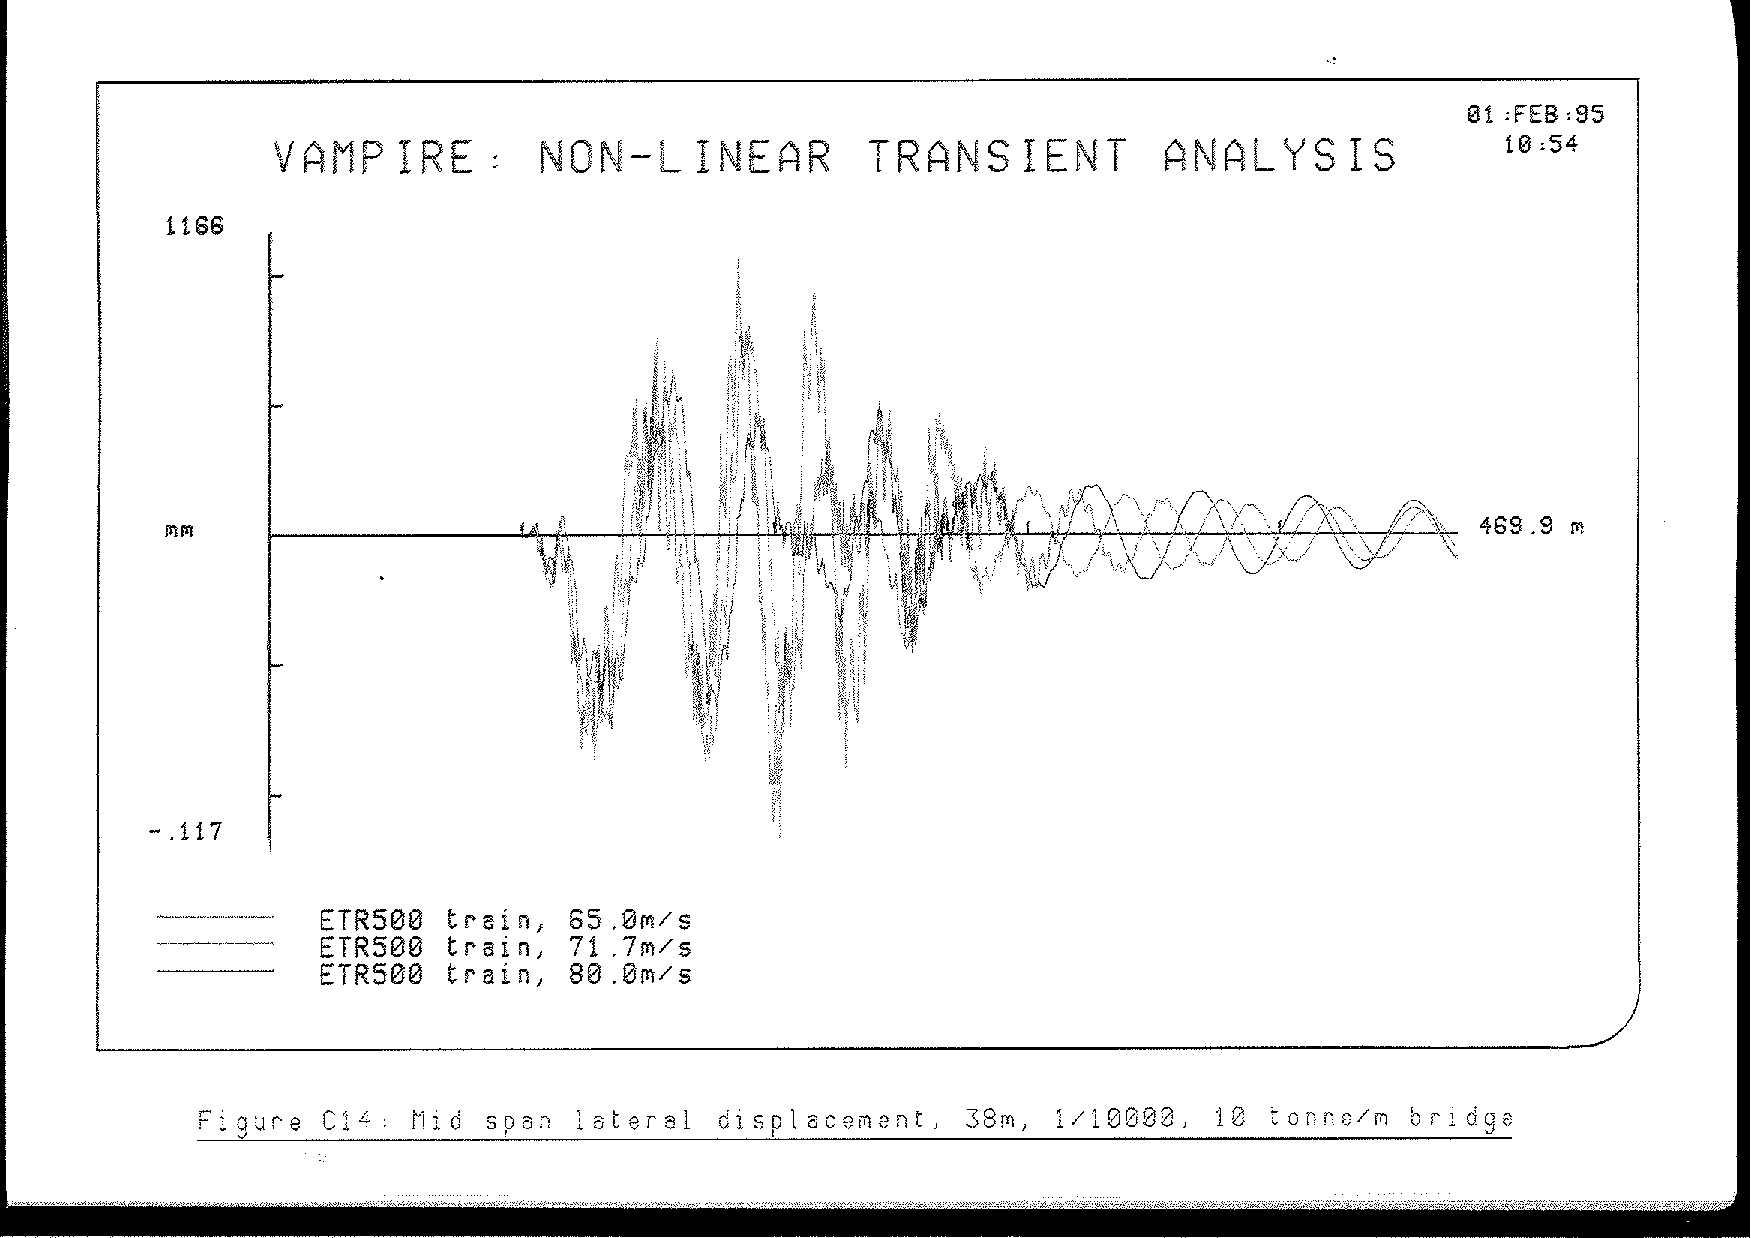
\includegraphics[width=0.8\textwidth]{c14}
    \caption{Figure C14 extracted from \citet{d181dt329}. An minor error is observed in y-axis label. Upper boundary of y-axis should be 0.116 }
    \label{fig:c14}
\end{figure}

To assure conservative comparison, only axle repeat pattern resonance results are selected because their output are more pronounced than kinematic resonance effect. Altogether 5 sets of reference data are selected. They include 2 reference data for freight trains(C3,C9), 2 reference data for passenger train(C12,C13) and 1 reference data for high-speed train(C14). Due to the fact that freight trains yield greater force than the other two types of trains, the analytical result should be conservative for the latter 3 cases. Since the output of C3 and C9 are already presented in Table.\ref{tab:parametersetupsandequivalentforce} so they are not being presented with other 3 sets of data this time. The bridge parameters and trains speed involved in these 3 cases(C12,C13,C14) are input into the analytical solution to yield analytical results.

\begin{table}[h!]
    \centering
    \caption{Comparison of results of simulation output and analytical output using refined load model}
    \begin{tabular}{c|ccc}
        \hline
         & C12 & C13 & C14\\
        \hline
        Stiffness($\sfrac{\delta_0}{t}$) & 1/10000 & 1/12000 & 1/10000\\
        Span($m$) & 54 & 54 & 38\\
        Mass per unit length($kg/m$) & 6000 & 6000 & 10000\\
        Speed of train($m/s$) & 55.6 & 55.6 & 65\\
        Damping ratio & 1\% & 1\% & 1\%\\
        Train type & Passenger & Passenger & High speed \\
        Track & Passenger Track & Passenger Track & High speed track\\
        \hline
        Peak Simulation displacement($mm$) & 1.48 & 1.41 & 0.117\\
        Peak Analytical displacement($mm$) & 6.6 & 5.8 & 3.0 \\
        \hline
    \end{tabular}
    \label{tab:comparisonresultssimulationanalytical}
\end{table}


In Table.\ref{tab:comparisonresultssimulationanalytical} the parameters involved in these 3 cases and their corresponding peak analytical results as well as peak simulation results are presented. 



\begin{figure}[h!]
\centering
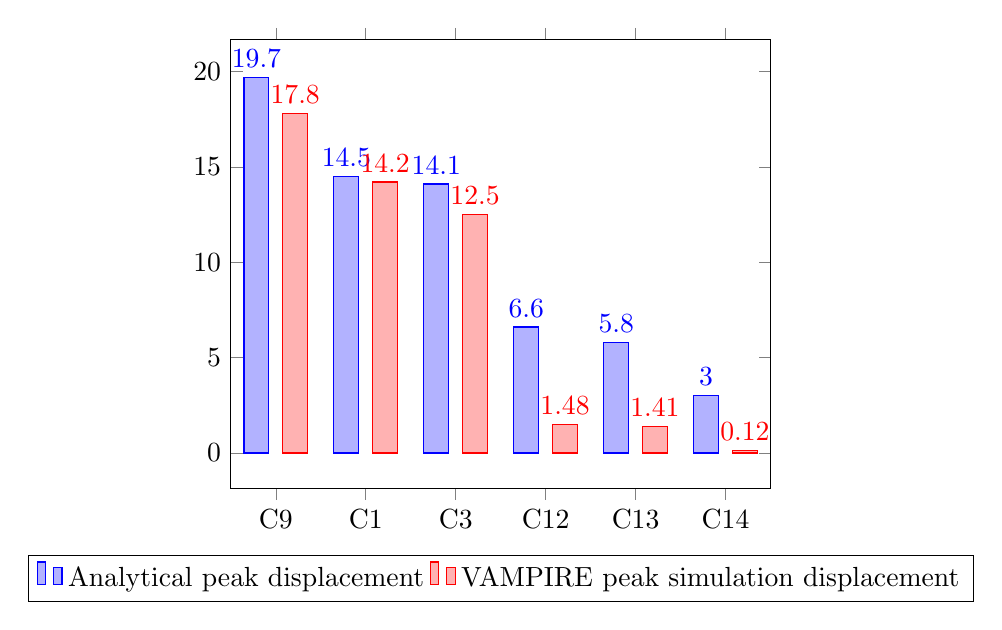
\begin{tikzpicture}
\begin{axis}[
    symbolic x coords={C9,C1,C3,C12,C13,C14},
    xtick=data,
    legend style={at={(0.5,-0.15)},
        anchor=north,legend columns=-1},
    ybar=5pt,% configures `bar shift'
    bar width=9pt,
    nodes near coords,
]
\addplot 
    coordinates {(C9, 19.7) (C1, 14.5) (C3, 14.1)   (C12,6.6) (C13,5.8) 
        (C14, 3.0) };
\addplot 
    coordinates {(C9, 17.8) (C1, 14.2) (C3, 12.5)  (C12,1.48) (C13,1.41)
         (C14,0.117) };
\legend{Analytical peak displacement,VAMPIRE peak simulation displacement}
\end{axis}
\end{tikzpicture}
\caption{Comparison between VAMPIRE peak simulation result and analytical peak result}
\label{fig:comparisonpeaksimulationanalytical}
\end{figure}

To clearer illustrate the comparison of both peak results from simulation and analytical, Figure.\ref{fig:comparisonpeaksimulationanalytical} is created with rearranged x-axis order to make the descending trend more obvious. Please note all data sets except for C1 are valid for verification(C1 is used in creation of expression).

It can be seen that analytical results always keep a conservative margin above the simulation results. As expected, margins for C12,C13,C14 are bigger compared to C9,C1,C3 proofs that the analytical solution becomes more conservative if adopted to passenger train and high-speed train. What's more, the descending trend of analytical results follows the descending trend of simulation results perfectly regardless of train types. Thus considering these reasons, the analytical solution is sufficient for universal application on all train types.

\section{Equivalent load amplitude created using every other setup available}
Although the equivalent load amplitude using C1 as reference has been created, the result is not valid yet because C1 is equivalent to other 5 setup scenarios(C3,C9,C12,C13,C14). It is also necessary to carry out the same calculating process on other 5 setup scenarios.

Taking advantage of the process developed during the creation of C1 equivalent amplitude, the load equivalent amplitude of other 5 setups are calculated and then presented in the Table.\ref{tab:allLoadEquivalentAmplitude}.

\begin{table}[h!]
    \centering
    \caption{Load equivalent amplitude(N) from all available setups}
    \begin{tabular}{cccccc}
        \hline
        C1 & C3 & C9 & C12 & C13 & C14 \\
        \hline
        1928 & 1721 & 1760 & 427 & 463 & 228 \\
        \hline
    \end{tabular}
    \label{tab:allLoadEquivalentAmplitude}
\end{table}

Their corresponding benchmarks are presented in Table.\ref{tab:allBenchmark}.

\begin{table}[h!]
    \centering
    \caption{Benchmark on analytical peak displacement generated by all equivalent load amplitude by comparing simulation peak displacement}
    \begin{tabular}{ccccccc}
        \hline
        Analytical Peak Displacement & C1 & C3 & C9 & C12 & C13 & C14 \\
        \hline
        C1 & 0.0145 & 0.0141 & 0.0197 & 0.0066 & 0.0058 & 0.0003 \\
        C3 & 0.013 & 0.0125 & 0.0174 & 0.0059 & 0.0051 & 0.0036 \\
        C9 & 0.013 & 0.0128 & 0.0178 & 0.0061 & 0.0053 & 0.0032 \\
        C12 & 0.0032 & 0.0031 & 0.0043 & 0.00148 & 0.0013 & 0.0008 \\
        C13 & 0.0035 & 0.0034 & 0.0047 & 0.0016 & 0.00141 & 0.0002 \\
        C14 & 0.0021 & 0.0020 & 0.0028 & 0.0010 & 0.0008 & 0.00012 \\
        \hline
        Simulation Peak Displacement & 0.0014 & 0.0125 & 0.0178 & 0.00148 & 0.00141 & 0.00012 \\
        \hline
        \label{tab:allBenchmark}
    \end{tabular}
\end{table}

Among all the equivalent load amplitude, the one created from C1 is most satisfying because its all outputs are conservative towards simulation output. Other equivalent load amplitude shows at least one nonconservative output. 

It can also be observed that the results of C12,C13,C14 are unacceptable due to the reason that their magnitude are too small. They can't predict reliable result for (C1,C3,C9). Their corresponding equivalent load amplitude will be ignored in the rest of the thesis.

Since there is few data available, it's meaningless to conduct further statistical procedures. The rest of the thesis will use the result of C1 because it's all conservative. However, the following section will give a simple guidance for statistical analysis provided by more simulations were done.

\section{Suggestions for further statistical analysis }

On the basis of more simulations could be conducted in the future, this section aims to give suggestions for further statistical analysis to improve the accuracy of the formula.

\paragraph{Filter out the influence of the parameters} It's essential to learn what roles are parameters playing in the simulation, so the simulations/analysis to be done should be planned ahead with a main objective which is  filtering out the influence on the bridge peak resonance displacement of the parameters such as bridge length, train speed, etc.

For example, by just looking at simulation peak displacement of C12,C13,C14, they are obviously small in magnitude compared to other 3. This is probably due to the reason that they all involve high speed train running. It could be that higher train speed tend to yield smaller deflection. However, this is only a hypothesis and needs more simulations to confirm.

\paragraph{Select correct statistical strategy} 

Content to be added after retrieving EN1990 Annex D.


\chapter{Finalizing the method for practical usage using real bridge parameters}

In practical usage, the speed that generates the highest peak response is unknown. Thus it is necessary to obtain the peak response for all speeds within the possible speed range. This is done by iterating the existing Matlab script with different speed. The increment in speed iteration is set in a way that ensures at least 1000 runs are done to guarantee precession. An example is illustrated as follows to show the usage on a real bridge project.

For an arch railway bridge located near Amsterdam, first step to is to collect following parameters:

$L = 255m$, $m = 5222e3kg$, $\mu = 2.0478e4 kg/m$, $EJ = 6.56e12Nm^2$

where:

$L$: span of the bridge

$\mu$: uniform mass per unit length of the bridge

$EJ$: lateral stiffness of the bridge

to test through a speed range of $1m/s - 30m/s$

Before beginning the calculation, make sure you have fog.m and Speedenvelop.m in your current working directory. By inputting following command in Matlab console, 

\texttt{Speedenvelop(6.56e12,255,2.0478e4,1,30,0.01)}


the envelop for displacement is generated and illustrated in Figure.\ref{fig:spedefEJ6560000000000L255min1max30mu20478.tikz}

\begin{figure}[h!]
\centering 
\newlength\figureheight 
\newlength\figurewidth 
\setlength\figureheight{6cm} 
\setlength\figurewidth{6cm} 
% This file was created by matlab2tikz v0.4.7 (commit 29117077607177efe915cc01d961cced006239c8) running on MATLAB 8.3.
% Copyright (c) 2008--2014, Nico Schlmer <nico.schloemer@gmail.com>
% All rights reserved.
% Minimal pgfplots version: 1.3
% 
\begin{tikzpicture}

\begin{axis}[%
width=\figurewidth,
height=\figureheight,
scale only axis,
xmin=0,
xmax=30,
ymin=0.0075,
ymax=0.011,
title={SpeedEnvelop def from1 to30}
]
\addplot [color=blue,solid,forget plot]
  table[row sep=crcr]{%
1	0.00781568842060085\\
1.2	0.00840892567977264\\
1.4	0.0088768875903958\\
1.6	0.00925769529057003\\
1.8	0.00957910144655464\\
2	0.00982648840148397\\
2.2	0.0100372557099215\\
2.4	0.0102060089657038\\
2.6	0.010347841028453\\
2.8	0.0104753362289414\\
3	0.010566090236029\\
3.2	0.0106426943938749\\
3.4	0.0107156879259678\\
3.6	0.0107656368912521\\
3.8	0.0108134770961416\\
4	0.0108433829006734\\
4.2	0.0108762461970553\\
4.4	0.0109009754438711\\
4.6	0.0109137058875431\\
4.8	0.0109063964703489\\
5	0.0109283926778865\\
5.2	0.0109354115709882\\
5.4	0.010934364378216\\
5.6	0.010925358882146\\
5.8	0.0109155184260617\\
6	0.0109160952245694\\
6.2	0.0109022893020932\\
6.4	0.0108894990281659\\
6.6	0.0108791296950589\\
6.8	0.0108683159097076\\
7	0.0108485530748728\\
7.2	0.0108354499334163\\
7.4	0.0108143121429067\\
7.6	0.0107967054438007\\
7.8	0.0107826189027167\\
8	0.0107571129205081\\
8.2	0.0107450192698353\\
8.4	0.0107182431373167\\
8.6	0.0107081009100856\\
8.8	0.0106810097968274\\
9	0.0106647893596357\\
9.2	0.0106368269751327\\
9.4	0.0106244435627288\\
9.6	0.0105902161380316\\
9.8	0.0105787489298167\\
10	0.0105530497685275\\
10.2	0.0105311301588914\\
10.4	0.0105155111529359\\
10.6	0.0104818416711415\\
10.8	0.0104658192794055\\
11	0.0104515232844051\\
11.2	0.0104195968460413\\
11.4	0.0103992383576141\\
11.6	0.0103875827376142\\
11.8	0.0103585518798102\\
12	0.0103282987036047\\
12.2	0.0103183620397562\\
12.4	0.0103012474040927\\
12.6	0.0102668977746374\\
12.8	0.0102449204320541\\
13	0.0102354809790005\\
13.2	0.0102169579397151\\
13.4	0.0101865143682396\\
13.6	0.0101530378665145\\
13.8	0.0101488592884028\\
14	0.0101342026283539\\
14.2	0.0101129828210581\\
14.4	0.0100781640001081\\
14.6	0.010051230942275\\
14.8	0.0100463931273211\\
15	0.0100339102223161\\
15.2	0.0100154789040376\\
15.4	0.00998674150551577\\
15.6	0.00995047989615967\\
15.8	0.00993544019804088\\
16	0.00993088834100722\\
16.2	0.0099199018939231\\
16.4	0.00990104705345698\\
16.6	0.00987441551082942\\
16.8	0.00984237739719204\\
17	0.00980928040956712\\
17.2	0.0098093242438416\\
17.4	0.00980329783311577\\
17.6	0.00979122702961792\\
17.8	0.00977314390458511\\
18	0.00974908670711774\\
18.2	0.00972108217302529\\
18.4	0.0096776691907686\\
18.6	0.00966812567615805\\
18.8	0.0096672743699076\\
19	0.00966167442250244\\
19.2	0.00965133478148734\\
19.4	0.00963626874305325\\
19.6	0.00961649393213872\\
19.8	0.00959203227865456\\
20	0.00956290998985286\\
20.2	0.0095021185042862\\
20.4	0.00950695108828918\\
20.6	0.00950797086177456\\
20.8	0.00950518266938973\\
21	0.00949859410737403\\
21.2	0.00948821551471712\\
21.4	0.00947405996230233\\
21.6	0.00945635016311157\\
21.8	0.00943490732597904\\
22	0.00940971735699768\\
22.2	0.00931048059107463\\
22.4	0.00931929357671497\\
22.6	0.00932536783564737\\
22.8	0.00932827887006457\\
23	0.00932803971339443\\
23.2	0.00932466491318731\\
23.4	0.00931817052503146\\
23.6	0.00930857410555171\\
23.8	0.00929589470449585\\
24	0.0092803683442182\\
24.2	0.00926243390849551\\
24.4	0.0092414380792758\\
24.6	0.00916278336234724\\
24.8	0.00909609061802426\\
25	0.00910564521095271\\
25.2	0.00911382028447303\\
25.4	0.00911959836984988\\
25.6	0.00912274595493189\\
25.8	0.00912328389307619\\
26	0.00912136767440461\\
26.2	0.00911807810466714\\
26.4	0.00911219402539695\\
26.6	0.00910373969614448\\
26.8	0.0090927400294876\\
27	0.00907945686157787\\
27.2	0.00906461860626204\\
27.4	0.00904726523290454\\
27.6	0.00902380873477224\\
27.8	0.00882644457839617\\
28	0.00883996385182427\\
28.2	0.00885231633946435\\
28.4	0.00886244919403873\\
28.6	0.00887051931610704\\
28.8	0.00887784576510649\\
29	0.0088829756466977\\
29.2	0.00888593368675971\\
29.4	0.00888785865101469\\
29.6	0.00888798738354364\\
29.8	0.00888597303168551\\
30	0.00888235391855735\\
};
\end{axis}
\end{tikzpicture}% 
\caption{Peak deflection at mid-span with regard to changing train speed. Parameters: $EJ = 6.56e12Nm^2$, $L= 255m$,$\mu = 20478 kg/m$, $c_{min}=1m/s$, $c_{max} = 30m/s$} 
\label{fig:spedefEJ6560000000000L255min1max30mu20478.tikz} 
\end{figure}

The plot shows that the critical speed appears at approximately $5m/s$ and corresponding peak deflection response is approximately $11mm$. 

Since the relationship between end support rotation angle and mid-span deflection is widely known as:

$$ \varphi = \frac{3}{L}\cdot \delta_0  $$

and rotation is yielded as:

$$ \varphi = \frac{3}{255}\times 0.011 = 0.00013 $$

This value is much lower than the rotation value regulated in EN1991-2. See Section.\ref{sec:Transverse-deformations-and-vibrations} for criteria details.

Thus the conclusion can be made that this bridge is safe subjected to lateral dynamic load.

However, if encountering unfavourable peak result, a filter can be applied on the train speed to further cut off the peak response. In previous chapter it has been already be concluded that all resonance effects between train and bridge are wavelength phenomenon. In order to couple frequency with bridge's first natural bending frequency, the train needs to operate at a certain speed range. 

For example, according to Chapter.\ref{sec:wavelengthstudy}, the possible wavelength range for trains in the Netherlands is approximately 10m-30m, including both axle repeat wavelength and kinematic wavelength. 

The natural frequency of the bridge in this example is 

$$ f_1 = \frac{\pi}{2l^2}\sqrt{\frac{EJ}{\mu}} = \frac{\pi}{2\times 255^2}\sqrt{\frac{6.56e12}{1.0478e4}} = 0.4Hz$$

so the possible resonance speedis obtained by multiplying wavelength range with natural frequency, yielding: $4m/s$ and $12m/s$

Although this speed filtering range doesn't help to cut off maximum response in this case because critical speed stills remains in the speed range, the filter can be more effective for bridges possessing higher first natural frequency simply because both lower and upper boundary for speed filtering range is linear to beam's first natural frequency. While it's not likely for upper boundary to shift to the left side of the critical speed, it's more favourable for lower boundary to shift to the right side of the critical speed.

\section{Conclusion}

The new practical method for checking lateral resonance response of railway bridge is developed in this chapter. This method is capable to simulate a resonance scenario where the bridge was passed by a moving railway vehicle. 

The method shows conservative prediction compared to VAMPIRE simulations. However, since lack of data can be used to further verify the practical method, results on longer span bridges can not be verified until new simulations or measurements data are obtained.

A general conclusion in finalizing phase of practical method is, for a certain bridge, faster train speed doesn't necessary cause higher resonance response of the bridge. As can be seen in Figure.\ref{fig:spedefEJ6560000000000L255min1max30mu20478.tikz}, critical speed appears at approximately $5m/s$, and response start to fall when speed is higher than $5m/s$. This means comparing to higher load amplitude caused by higher train speed, the shorter loading time caused by same reason is more dominating. By considering the fact in Figure.\ref{fig:comparisonpeaksimulationanalytical} that the analytical is even more conservative for higher speed, it can be concluded than high-speed trains cause less dynamic problem for lateral bridge dynamics.

Matlab scripts are already written and attached for the convenience of readers. Since the explicit solution has been given in the chapter, it's completely possible to adopt them in other mathematical software for different preferences.

\chapter{Conclusion}


Two proposed criteria in RP6\citet{d181} were adopted in Eurocode 1991-2. One of them is 1.2Hz criterion. It was adopted without amending. The other one is lateral force models. Loading models were adopted in a different name as 'nosing force' in \citet[A6.5.2]{EC12}. 

\begin{enumerate}[-]
\item The 1.2Hz criterion was aiming to avoid the occurrence of resonance between bridge first lateral vibration mode and vehicle sway mode, however, no research can be found among all D181 report series to support this hypothesis. This criterion was proposed without a valid background.

\item Nosing force in EN1991-2 has a single characteristic value of 100kN, while RP6 proposes different values for different scenarios. Also, it is proved that nosing force isn't conservative when resonance happens between the vehicle and the bridge.
\end{enumerate}

In addition, D181 did research on other 2 resonance phenomenons, including axle repeat pattern resonance and kinematic movement resonance. Resonance was proofed to be possible and was successfully reproduced using VAMPIRE software. These two resonance are wavelength phenomenon, meaning resonance can happen on any train/bridge combination.

However, the dynamic effects start to build up at a broader frequency, which means even if the resonance is avoided between bridge and train, the response of the bridge will still be amplified by dynamic loading. The relationship between total peak lateral force of the first two traction units and speed is found by using the simulation output and regression approach. The lateral force is greatly dependant on track quality, train type and speed.

Nosing force model was proposed by investigating the peak lateral force on track with a standard deviation of 7mm. Such track irregularities ensures the occurrence of hunting effects thus this value is conservative. However, for tracks maintained as regulation requires, up to 2mm standard deviation is allowed. Since track force increases as track standard deviation does, it can be concluded that 100kN of characteristic value for nosing force is very conservative.

By using the knowledge above, a practical method for easy calculating real-time mid-span resonance responses of the bridge is also developed. The method features a analytical model and an equivalent amplitude model. The equivalent amplitude model is developed based on both the simulation result of VAMPIRE software and the relationship between lateral force and train speed discovered earlier in the report. The practical method shows reasonable conservative prediction when compared to other reference data in DT329 reports.

However, as VAMPIRE simulation results only have span up to 120m, there’s no benchmark can be found to validate the correctness of the formula for longer span inputs. So it is highly advisable that more simulations/measurements to be done to verify the correctness of result for longer span bridges.

\chapter{Recommandations on future reseraches}

Future reseaches to be proposed in this section are mainly related to heavy FEM transient analysis. Although D181 commiittee conducted a number of simulations in D181 report seriers, the response of longer span bridges remaines unknown. What's more, D181 report series were created in 1990's. The trains and their parameters used in the report are too old for nowadays usage.

The aim of proposed FEM simulations is to verify the practical method described in this thesis. The method is needed to be verified for longer span bridges and modern vehicle design. As a conclusion, simulations with following objectives are needed to be done:

\begin{enumerate}
    \item Lateral forces on tracks of modern vehicles/tracks
    \item Resonance response of bridges with span longer than 150m
\end{enumerate}

These simulations should be done with following extra requirements on the basis of simulations done in resonance study of DT329:

\begin{enumerate}
    \item More realistic and up-to-date data on modern train vehicles
    \item More realistic data on lateral track irregularities
    \item Broader range of bridge span to be investigated(greater than 150m)
\end{enumerate}

More accurate statistical result can be yielded with more simulation data. Since now only 6 sets of data can be used, the new practical method can hardly be globally reliable. However, it is recommended that future research uses a larger simulation data base to further improve the accuracy of the new method.

Transient simulations of this topic is very resource demanding. It is impossible for this thesis to carry out these simulations. Thus above simulations are proposed to whoever poceesing the resource and willingness to further investigate the topic. It is also proposed that lateral force data caused by running trains to be evaluated more frequently.

The practical method should be verified by comparing its own result with result of newly conducted simulations. The result of practical method should be conservative according to the comparison. 

It is possible to modify the amplitude in practical method to a less conservative value according to newly conducted simulations. It is expected that newly conducted simulations yield smaller lateral force on tracks because of the advanced suspension systems implemented in modern vehicle designs and better track quality.

%!TEX root = main.tex
\begin{appendices}

% \chapter{Basic concepts of railway bridge dynamics}

% In this chapter basic concepts of railway bridge dynamics will be described in order to provide preliminary relevant knowledge for following chapters. The knowledge will be introduced in the order of railway dynamics related only to bridge dynamics related. 

% \section{Basic railway dynamic effects}

% \subsection{Sources induce transverse dynamic reactions}
% According to \citet{da2007dynamic}, \citet{fryba1996dynamics} and \citet{EC12}, following sources are identified:

% \begin{enumerate} [-]
%     \item Sinusoidal motion of conical wheels along cylindrical rail heads. See Section.\ref{sec:klingel}
%     \item Horizontal track irregularities. See Section.\ref{sec:lateraltrackirrgularities}
%     \item Centrifugal forces on curved tracks. This source is not disccused because only straight tracks are discussed in this thesis.
%     \item Train switches. This source is not disccussed because of the same reasone as above item.
% \end{enumerate}

% \subsection{Lateral movement of a wheelset on straight track}

% Following knowledge in all subsections of this section is extracted from \citet{esveld2001modern}. 

% \subsubsection{Theory according to Klingel}\label{sec:klingel}

% \begin{quote}
% If a wheelset with conical tire profiles is laterally displaced from central position, this displacement is counteracted due to different rolling radii of the wheels. This results in a periodical movement of the wheelset which was described by Klingel in 1883 and is therefore often referred to as the Klingel movement. When analysing the case, the wheelset is modelled as a biconus travelling on an ideally straight track as shown in Figure.\ref{fig:wheelsetbiconus}

% \begin{figure}[h]
%     \centering
%     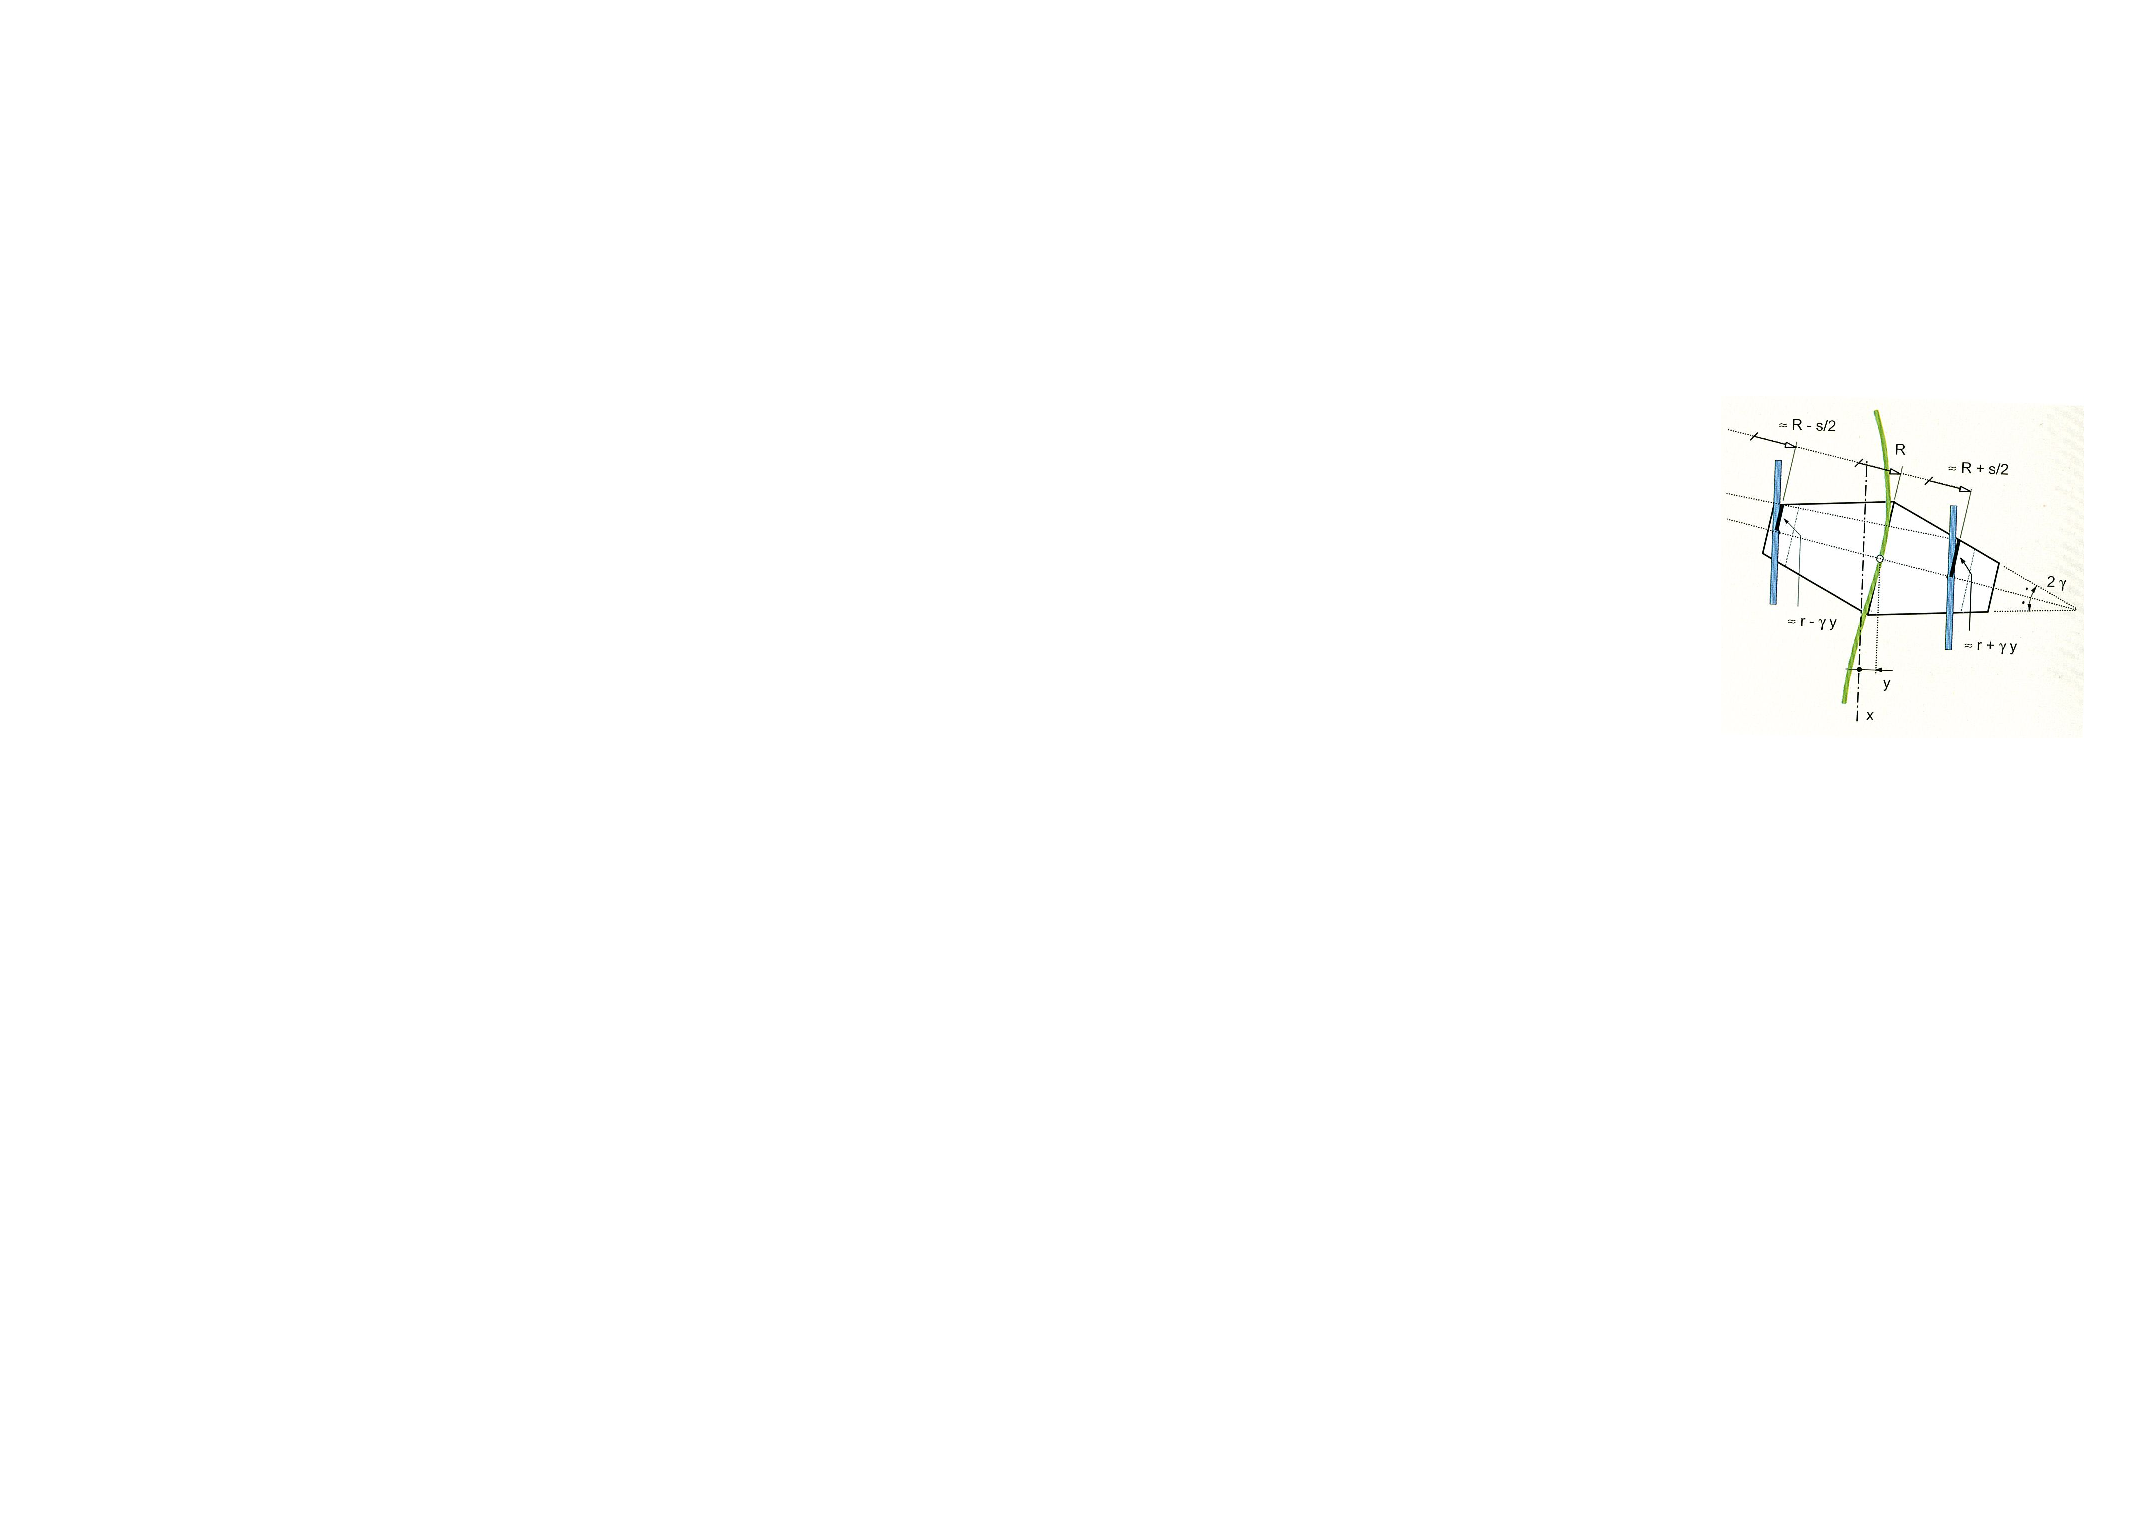
\includegraphics[width=0.5\textwidth]{wheelsetbiconus}
%     \caption{Wheelset biconus in general position. Extracted from \citet[Figure 2.2]{esveld2001modern}}
%     \label{fig:wheelsetbiconus}
% \end{figure}


% The Klingel movement is therefore purely a kinematic movement in which forces play no part in the derivation. As a result, Figure.\ref{fig:klingelmovement} visualizes the Klingel movement. The lateral displacement $y$ is a harmonic, undamped function of the distance co-ordinate $x$ as long as the amplitude moves within the flangeway clearance $fwc$. This is illustrated in Figure.\ref{fig:fwc}.

% \begin{figure}[h]
%     \centering
%     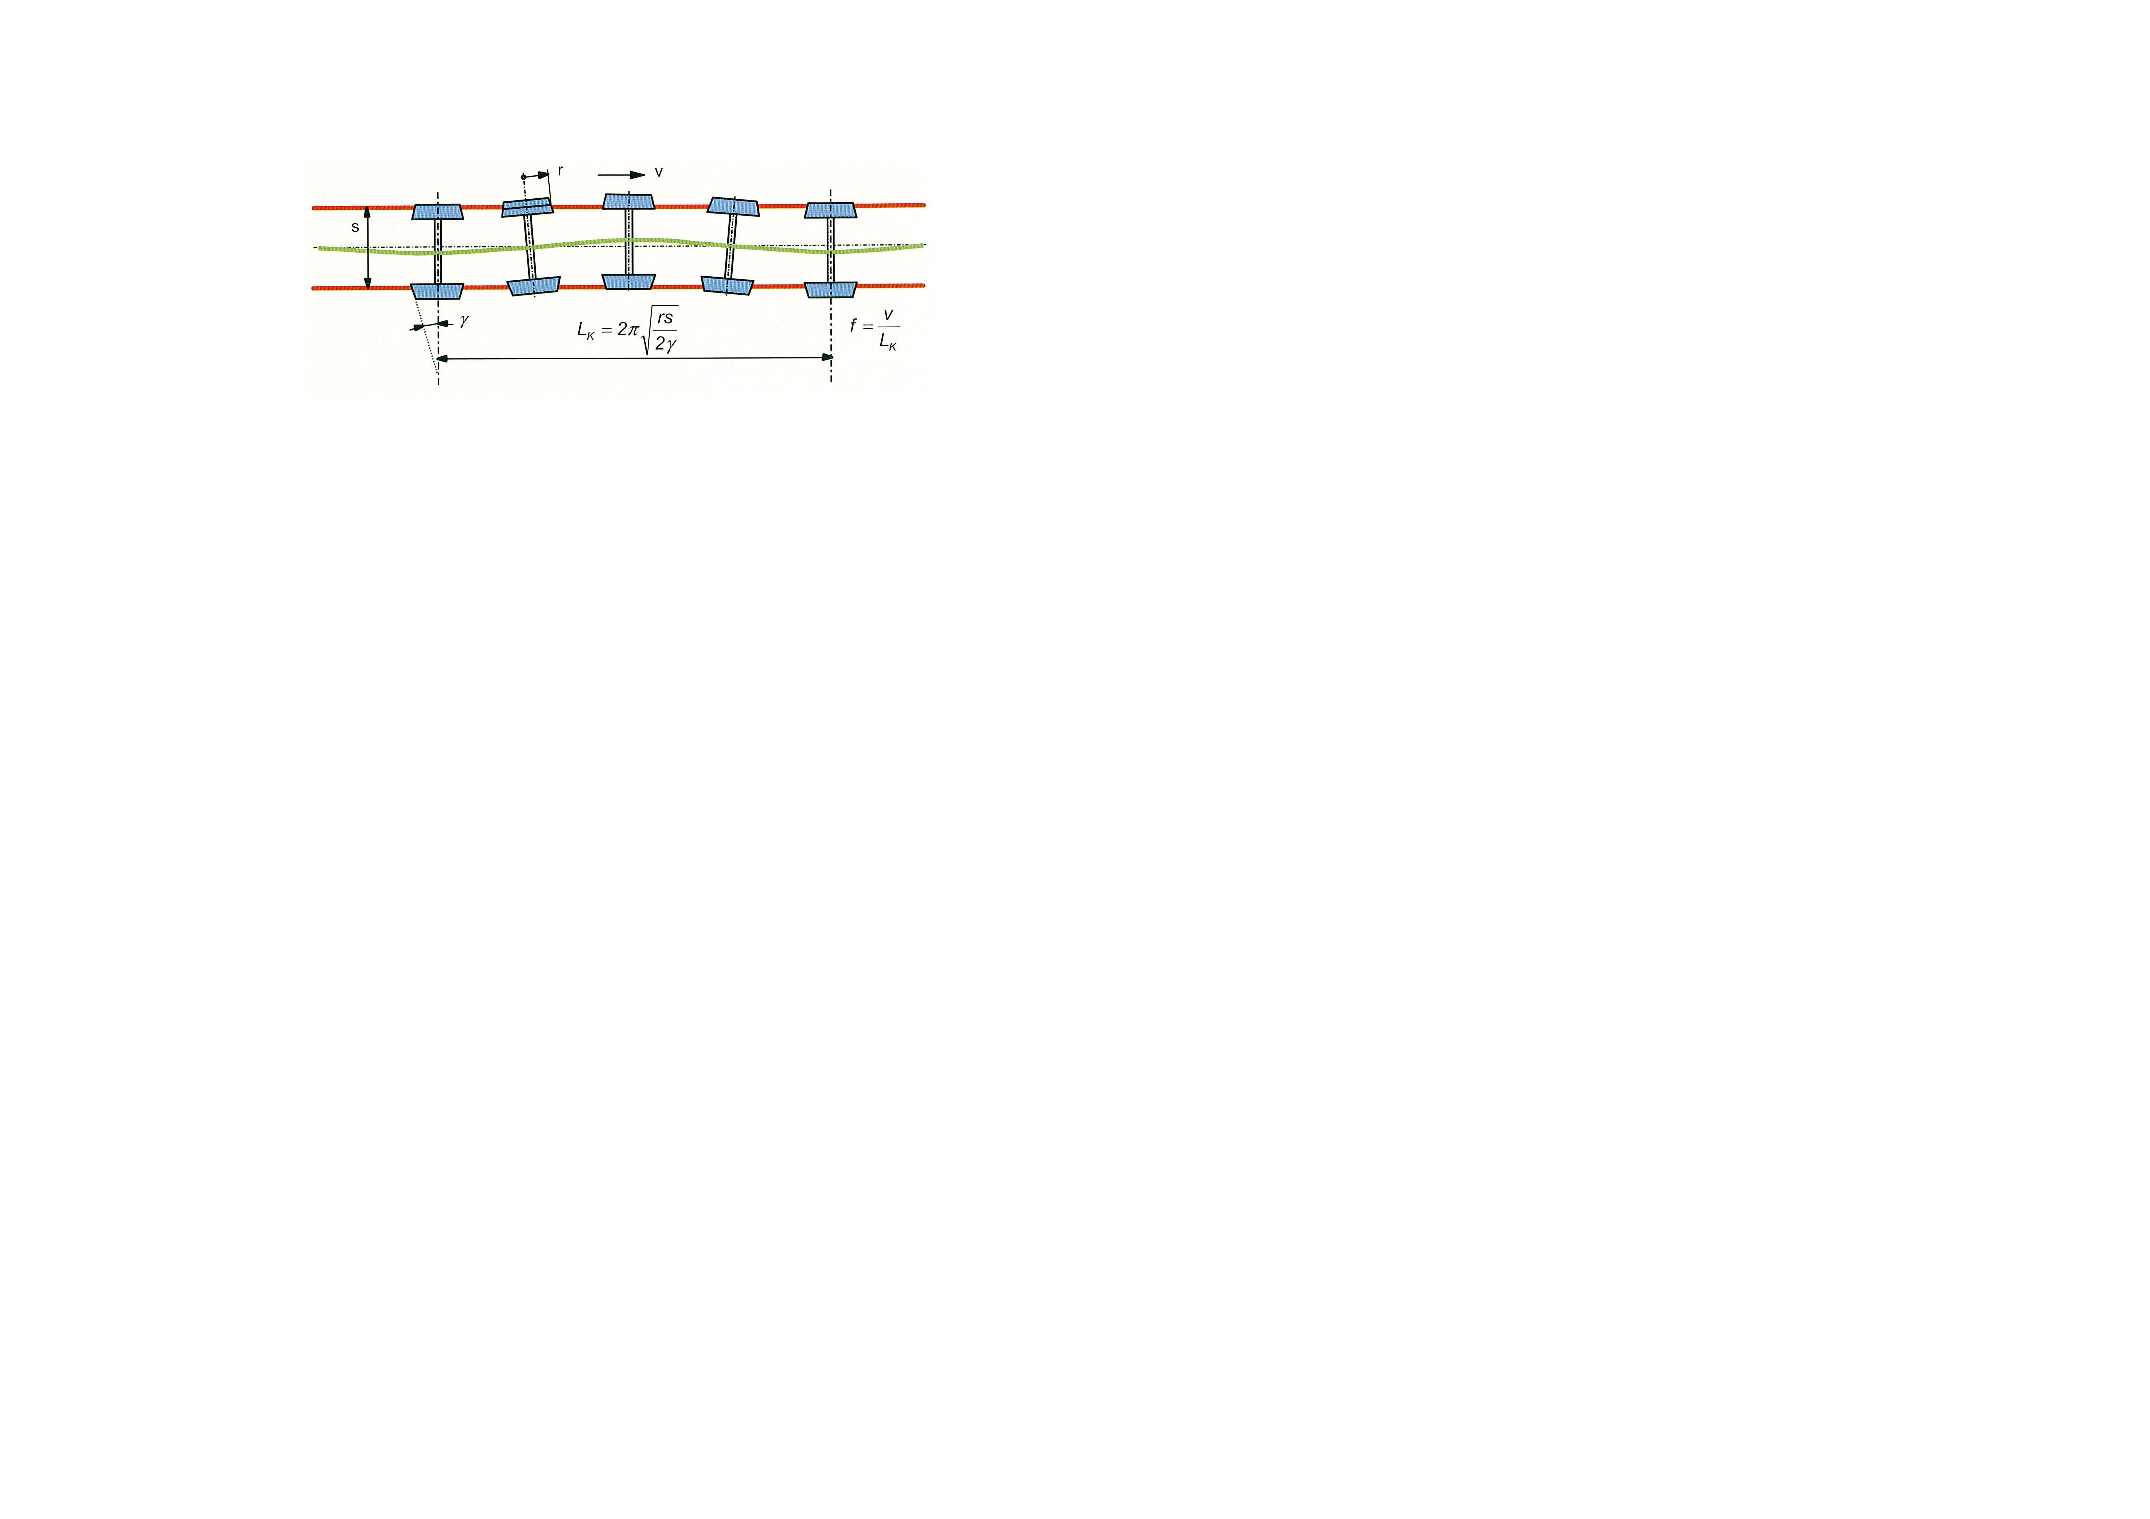
\includegraphics[width=0.8\textwidth]{klingelmovement}
%     \caption{Klingel movement. Extracted from \citet[Figure 2.3]{esveld2001modern}}
%     % \label{fig:klingelmovement}
% \end{figure}

% \begin{figure}[h]
%     \centering
%     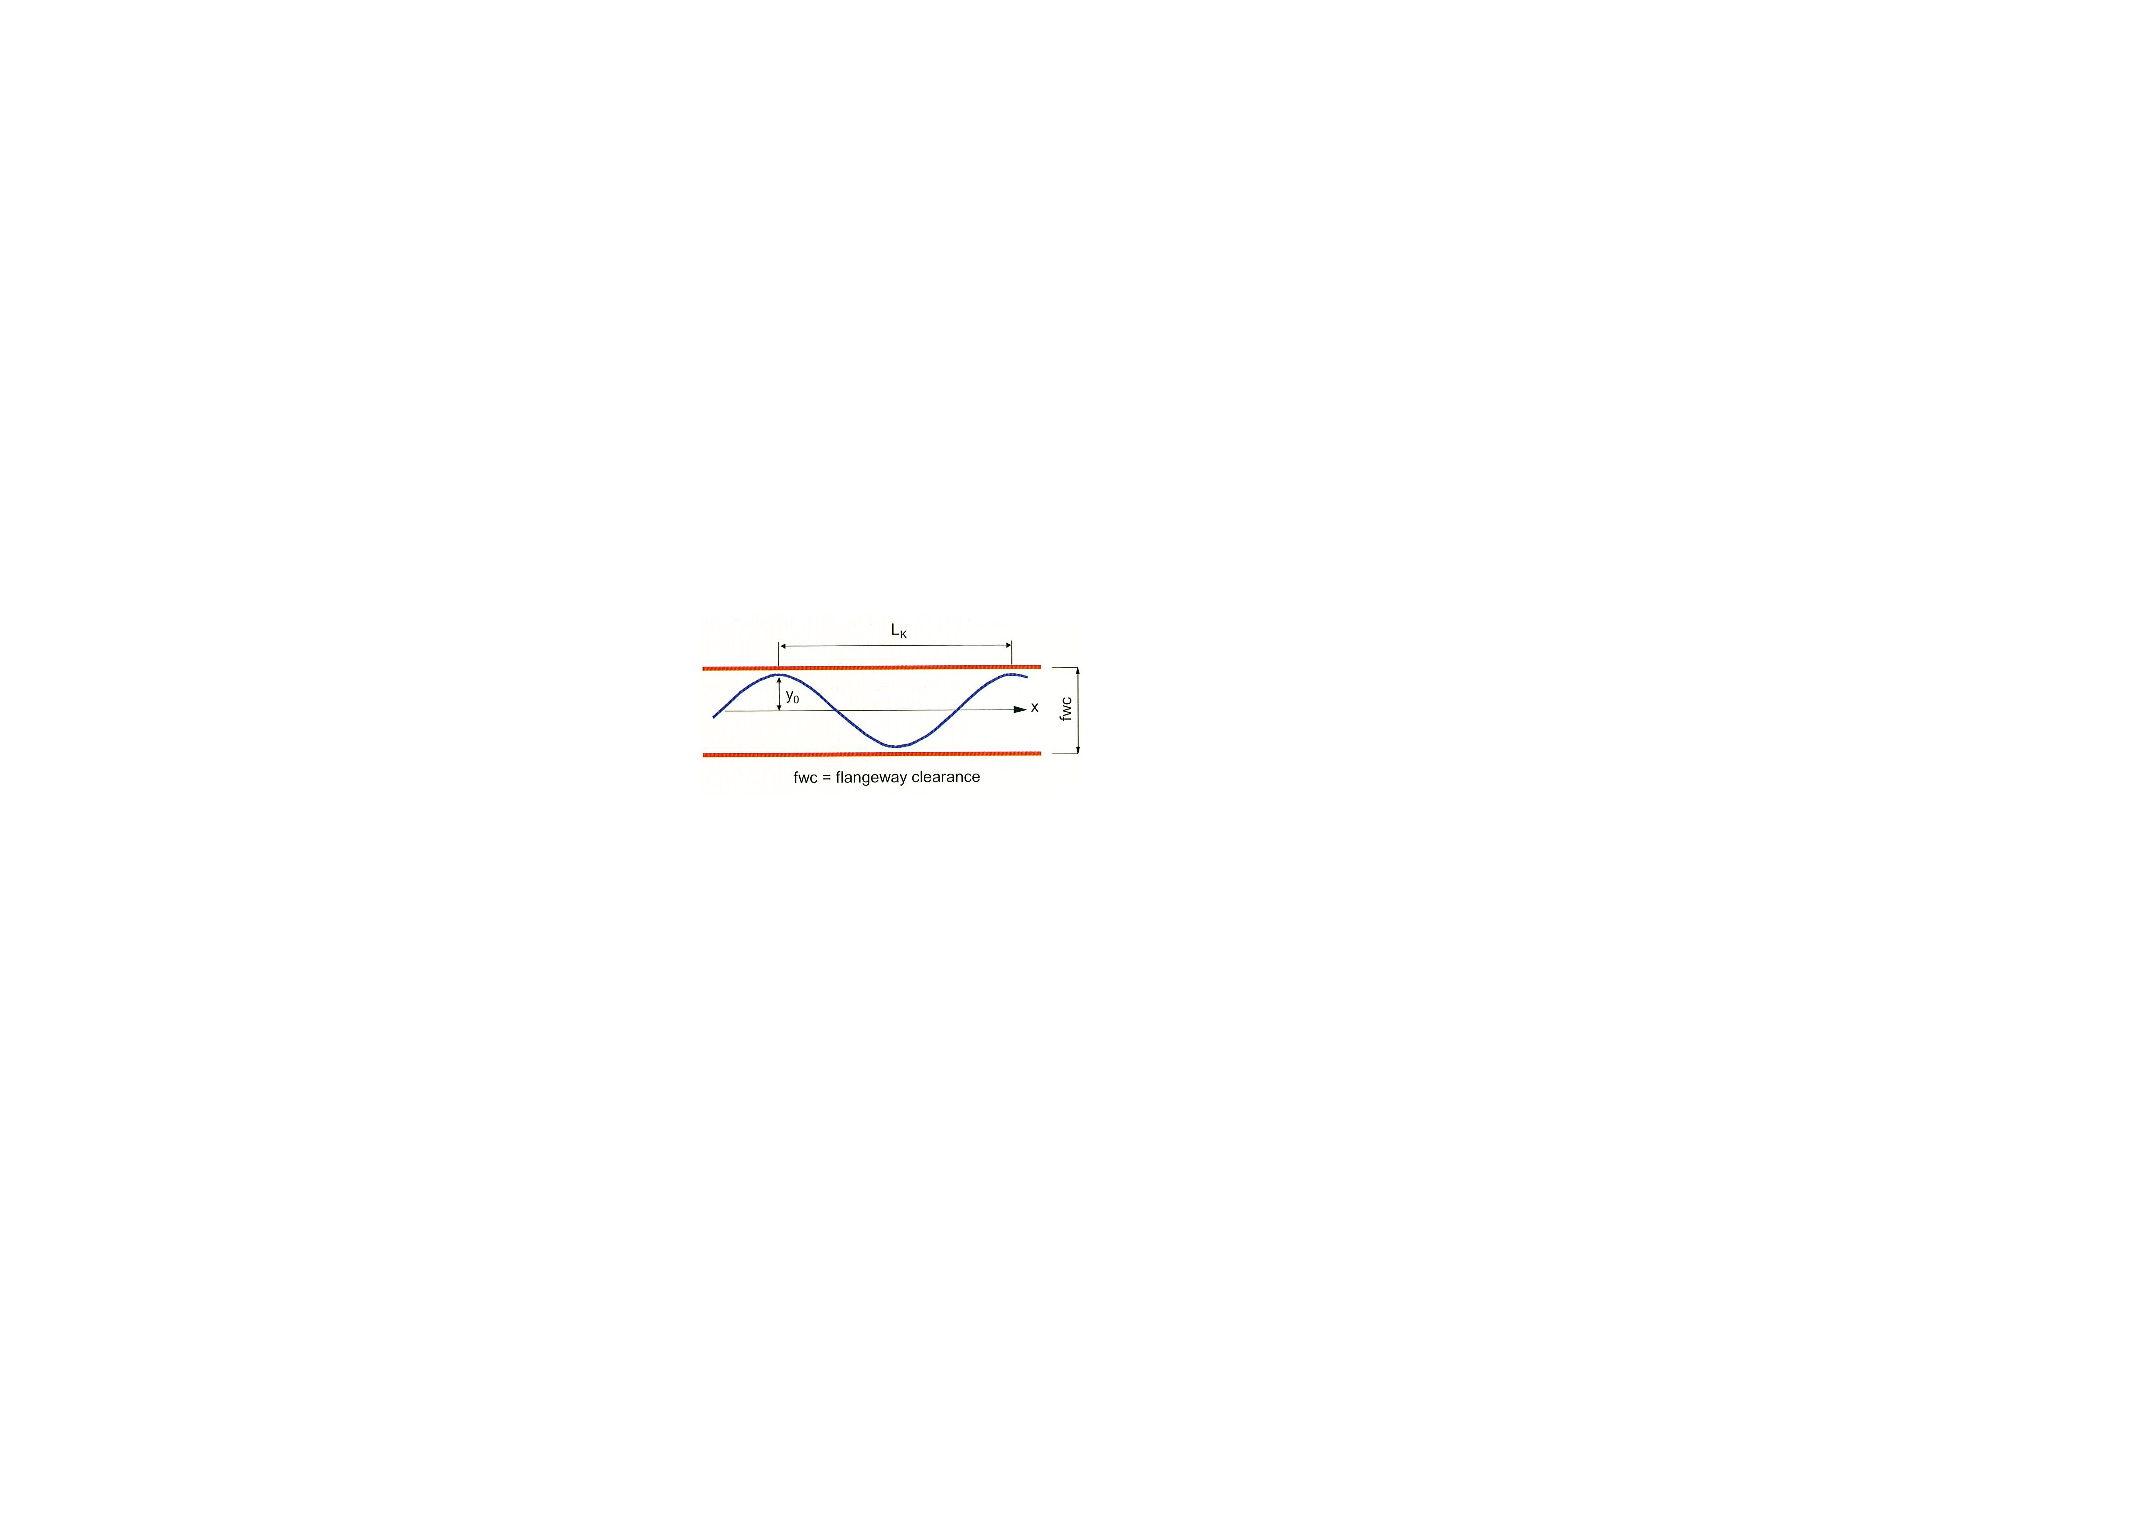
\includegraphics[width=0.5\textwidth]{fwc}
%     \caption{Undisturbed lateral movement of a wheelset. Extracted from \citet[Figure 2.4]{esveld2001modern}}
%     \label{fig:fwc}
% \end{figure}

% Introducing the speed, the time domain frequency of the Klingel movement is:

% $$ f = \frac{V}{L_k} $$

% and hence the maximum lateral acceleration can be calculated as:

% $$\ddot{y}_{max} = 4\pi^2y_0\frac{v^2}{L_k^2}$$

% If the frequency $f$ coincides with one of the natural frequencies of the rolling stock, the vehicle ride becomes unstable. The lateral acceleration, which is a measure of the forces, shows the adverse effect of high speed and/or small wavelength. A conicity, for example, of 1:40 in comparison with 1:20 therefore gives a greater wavelength and a lower lateral acceleration at the same speed. The progressively increasing conicity in the case of worn profiles due to increasing lateral axle movement, therefore, has an adverse effect in this respect.
% \end{quote}
% \subsubsection{Hunting movement}
% \begin{quote}
% It should be noted that the Klingel theory is simple and instructive but does not include the effect of coupled axes, mass forces, and adhension forces. In reality, the amplitude $y_0$ of the Klingel movement is dependent on alignment, dynamic vehicle behaviour, and the speed of the rolling stock. 

% Generally speaking, $y_0$ due to slip will increase with speed until it is equal to half the flangeway clearance. Flanging then occurs as a result of which the axle will rebound. 

% This means that the lateral movement takes on a completely different behaviour which is known as hunting. As shown in the drawing in Figure\ref{fig:flangingwheelset} the movement changes from a harmonic to a zig-zag shape. The wavelength becomes shorter and the frequency increases quickly until it is in the critical range for the rollin g stock and resonance occurs.

% \begin{figure}[h!]
%     \centering
%     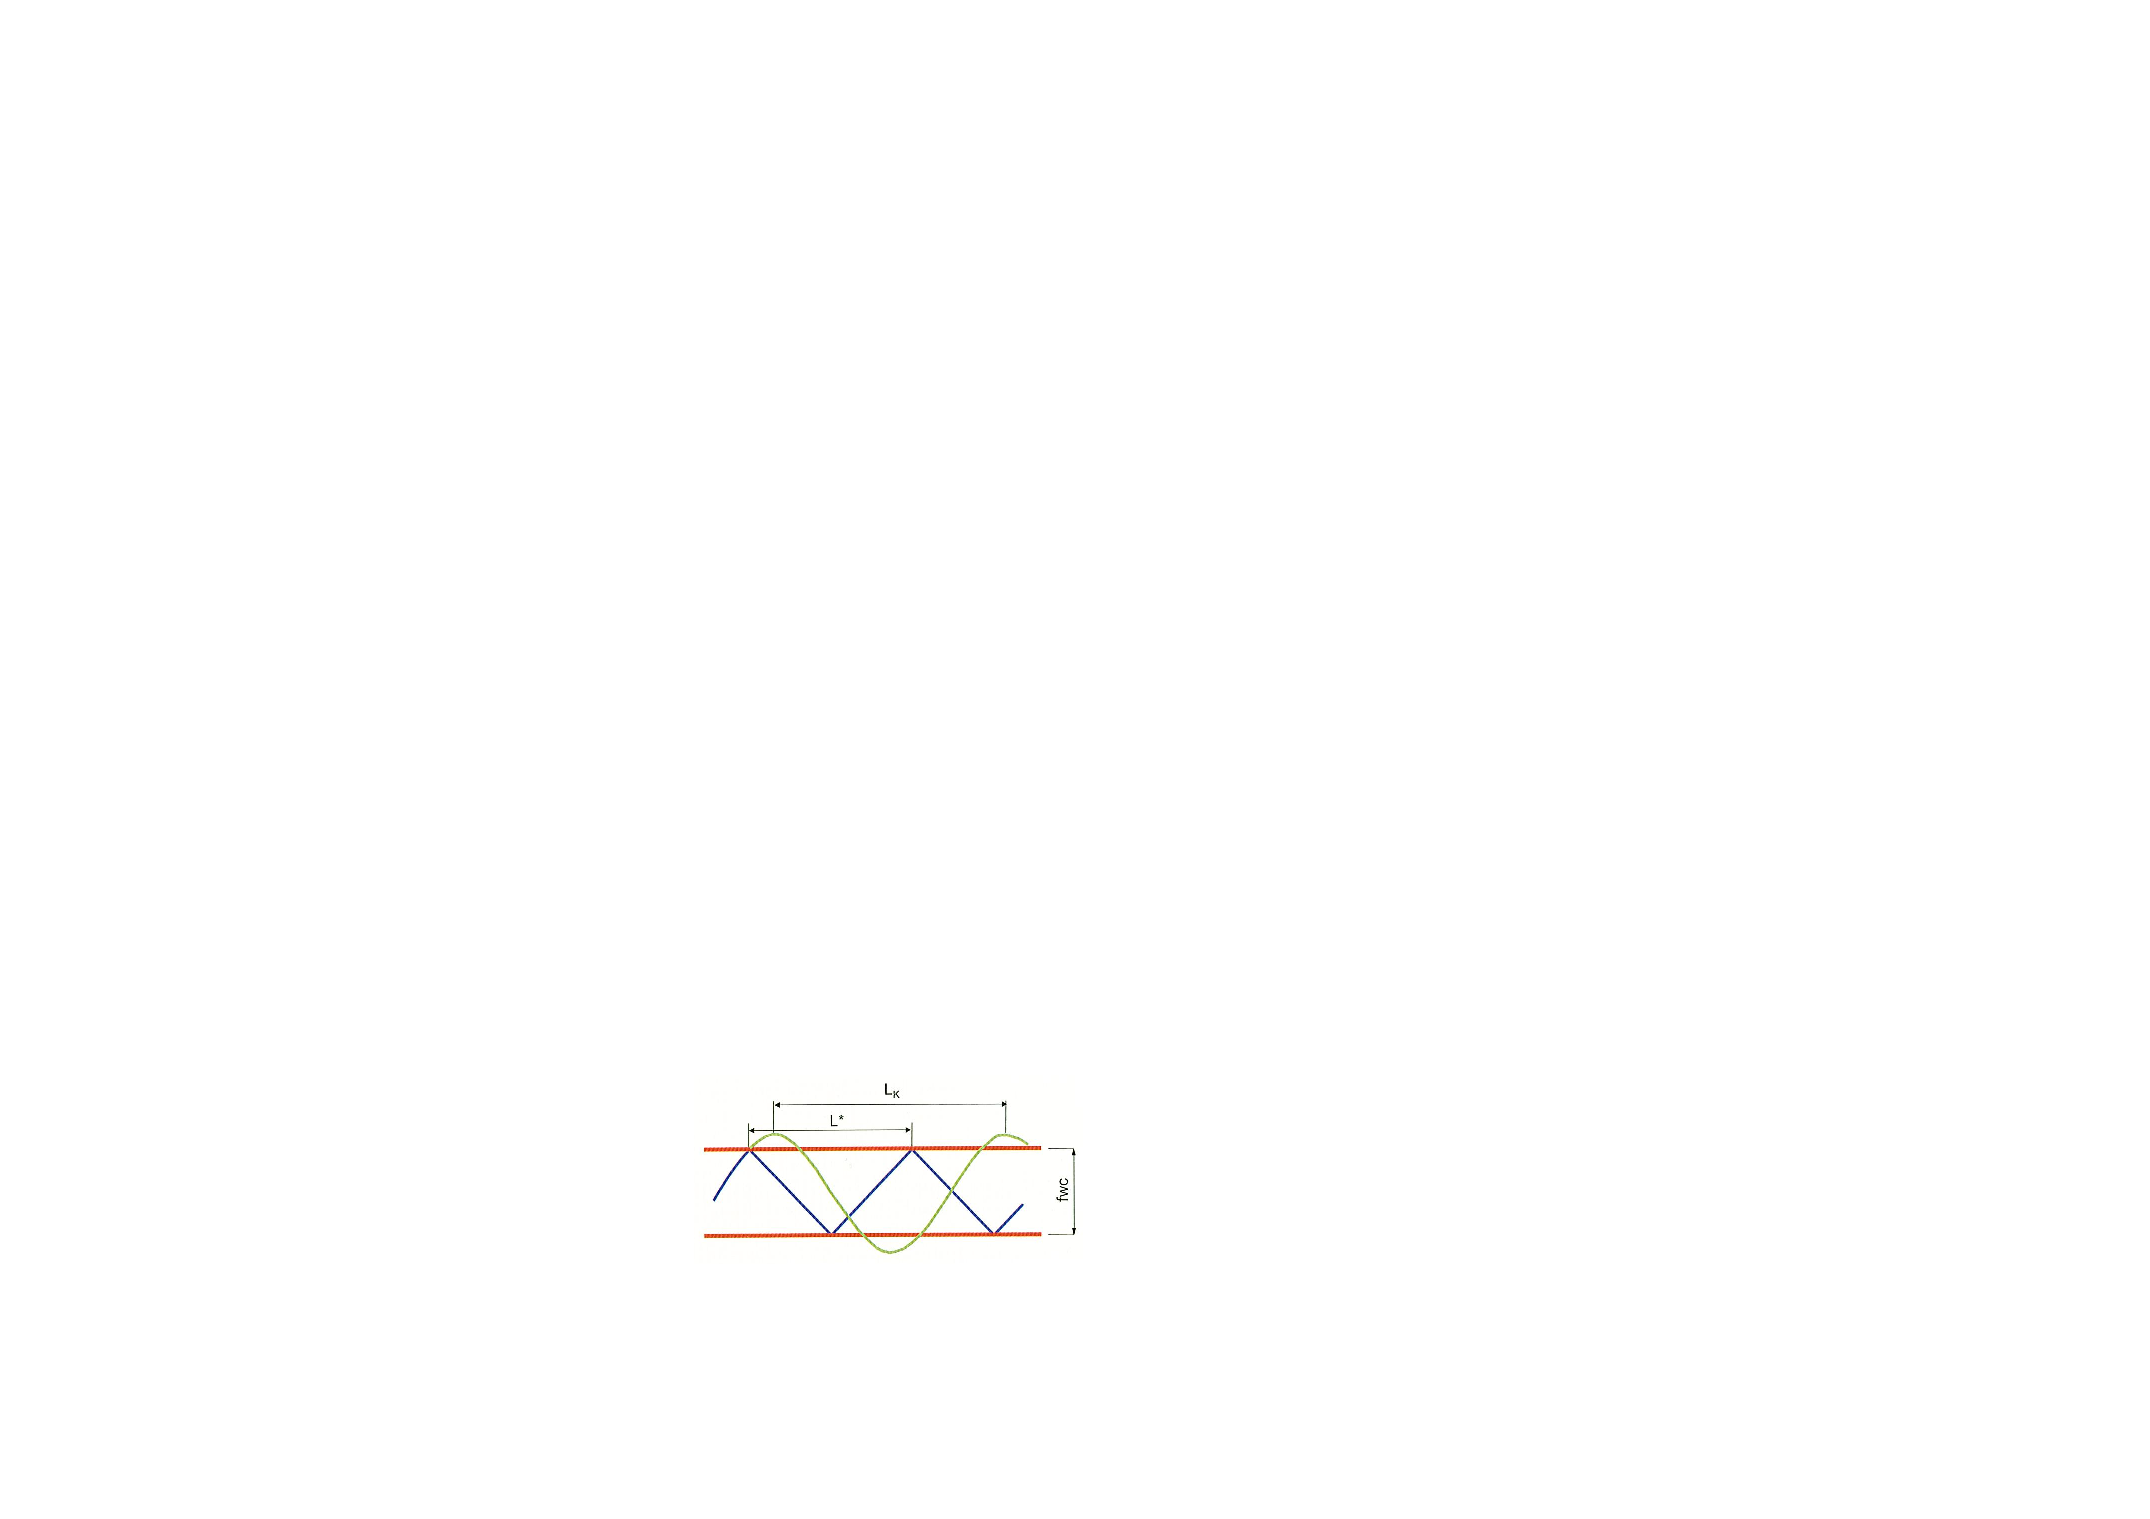
\includegraphics[width=0.5\textwidth]{flangingwheelset}
%     \caption{Influence of flanging on lateral wheelset movement. Extracted from \citet[Figure 2.5]{esveld2001modern}}
%     % \label{fig:flangingwheelset}
% \end{figure}

% This phenomenon is shown in Figure\ref{fig:amplitudefrequencystability}. The bogie design, as far as conicity and flangeway clearance are concerned, must be such that stable running is always guaranteed for the speed range in which the vehicle is to be used.


% \begin{figure}[h!]
%     \centering
%     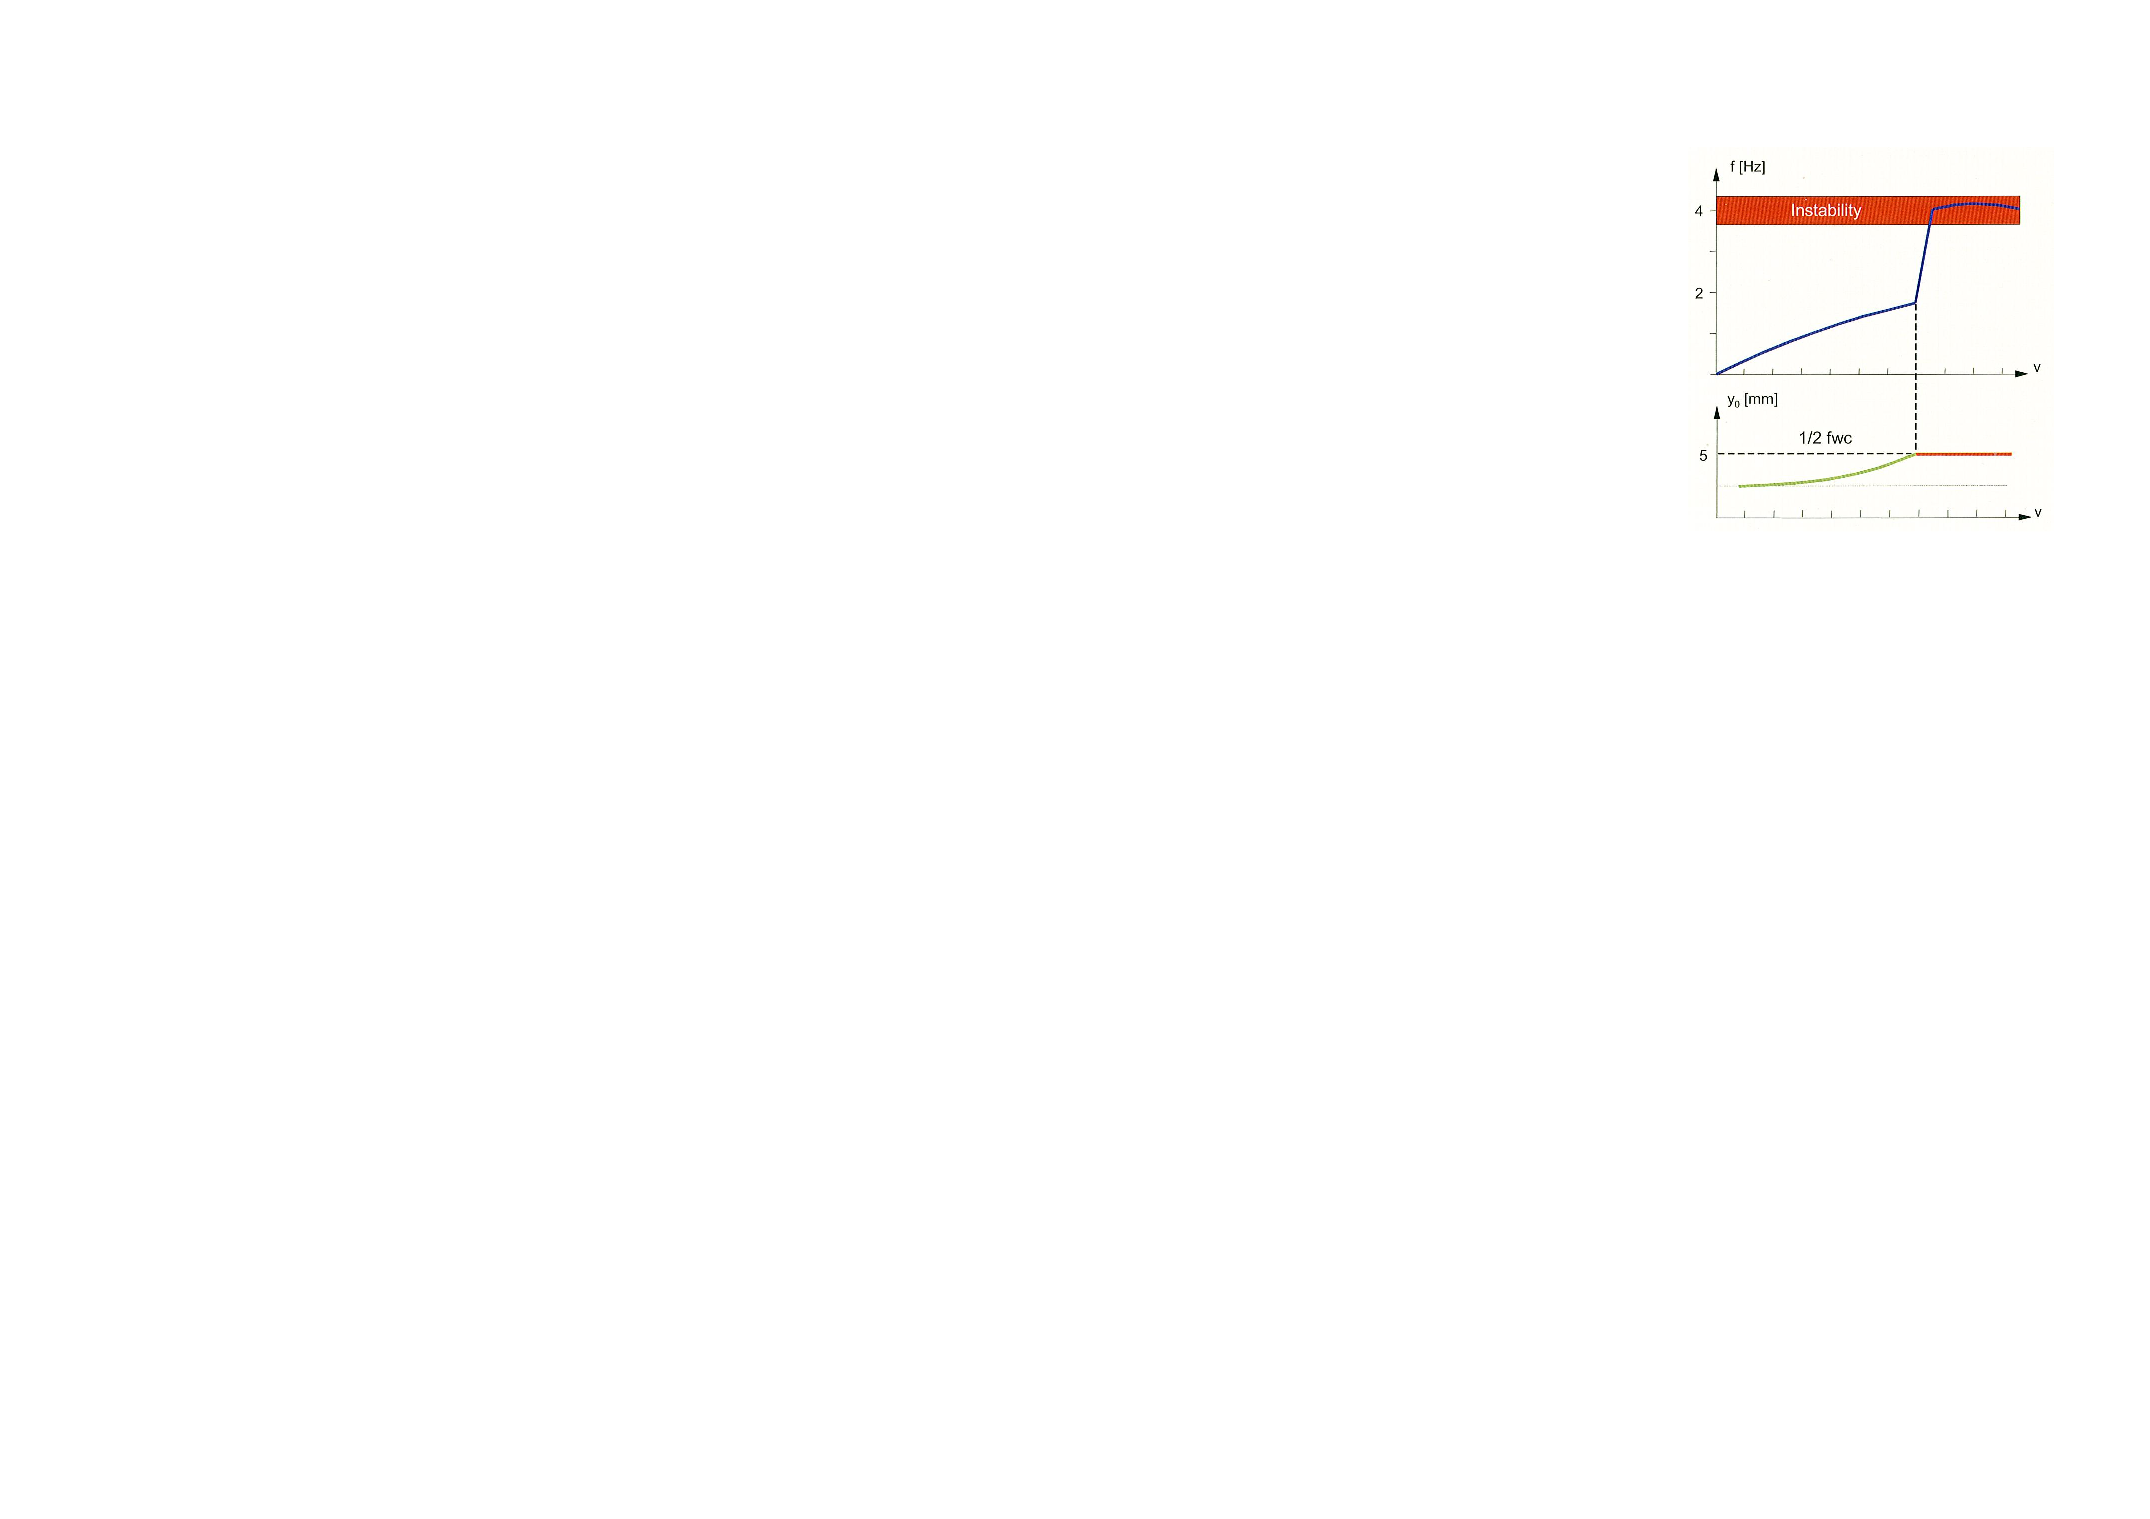
\includegraphics[width=0.5\textwidth]{amplitudefrequencyinstability}
%     \caption{Increase in amplitude and frequency with speed and the development of instability. Extracted from \citet[Figure 2.6]{esveld2001modern}}
%     \label{fig:amplitudefrequencystability}
% \end{figure}

% \subsection{Single and two-point contact between wheel and rail}
% In the case of single-point contact, according to Figure.\ref{fig:singlecontact}, wheel load and lateral force act on the same point. This situation occurs when using worn wheel profiles. In the case of two-point contact, shown in Figure.\ref{fig:doublecontract}, the application points do not coincide.

% Flanging occurs in the situation of double contact. 

% \begin{figure}[h!]
% \centering
%     \begin{subfigure}[b]{0.2\textwidth}
%         \centering
%         
\includegraphics[width=\textwidth]{singlecontact}
%         \caption{Single contact point.  Extracted from \citet[Figure 2.13]{esveld2001modern}}
%         \label{fig:singlecontact}
%     \end{subfigure}
%     \begin{subfigure}[b]{0.5\textwidth}
%         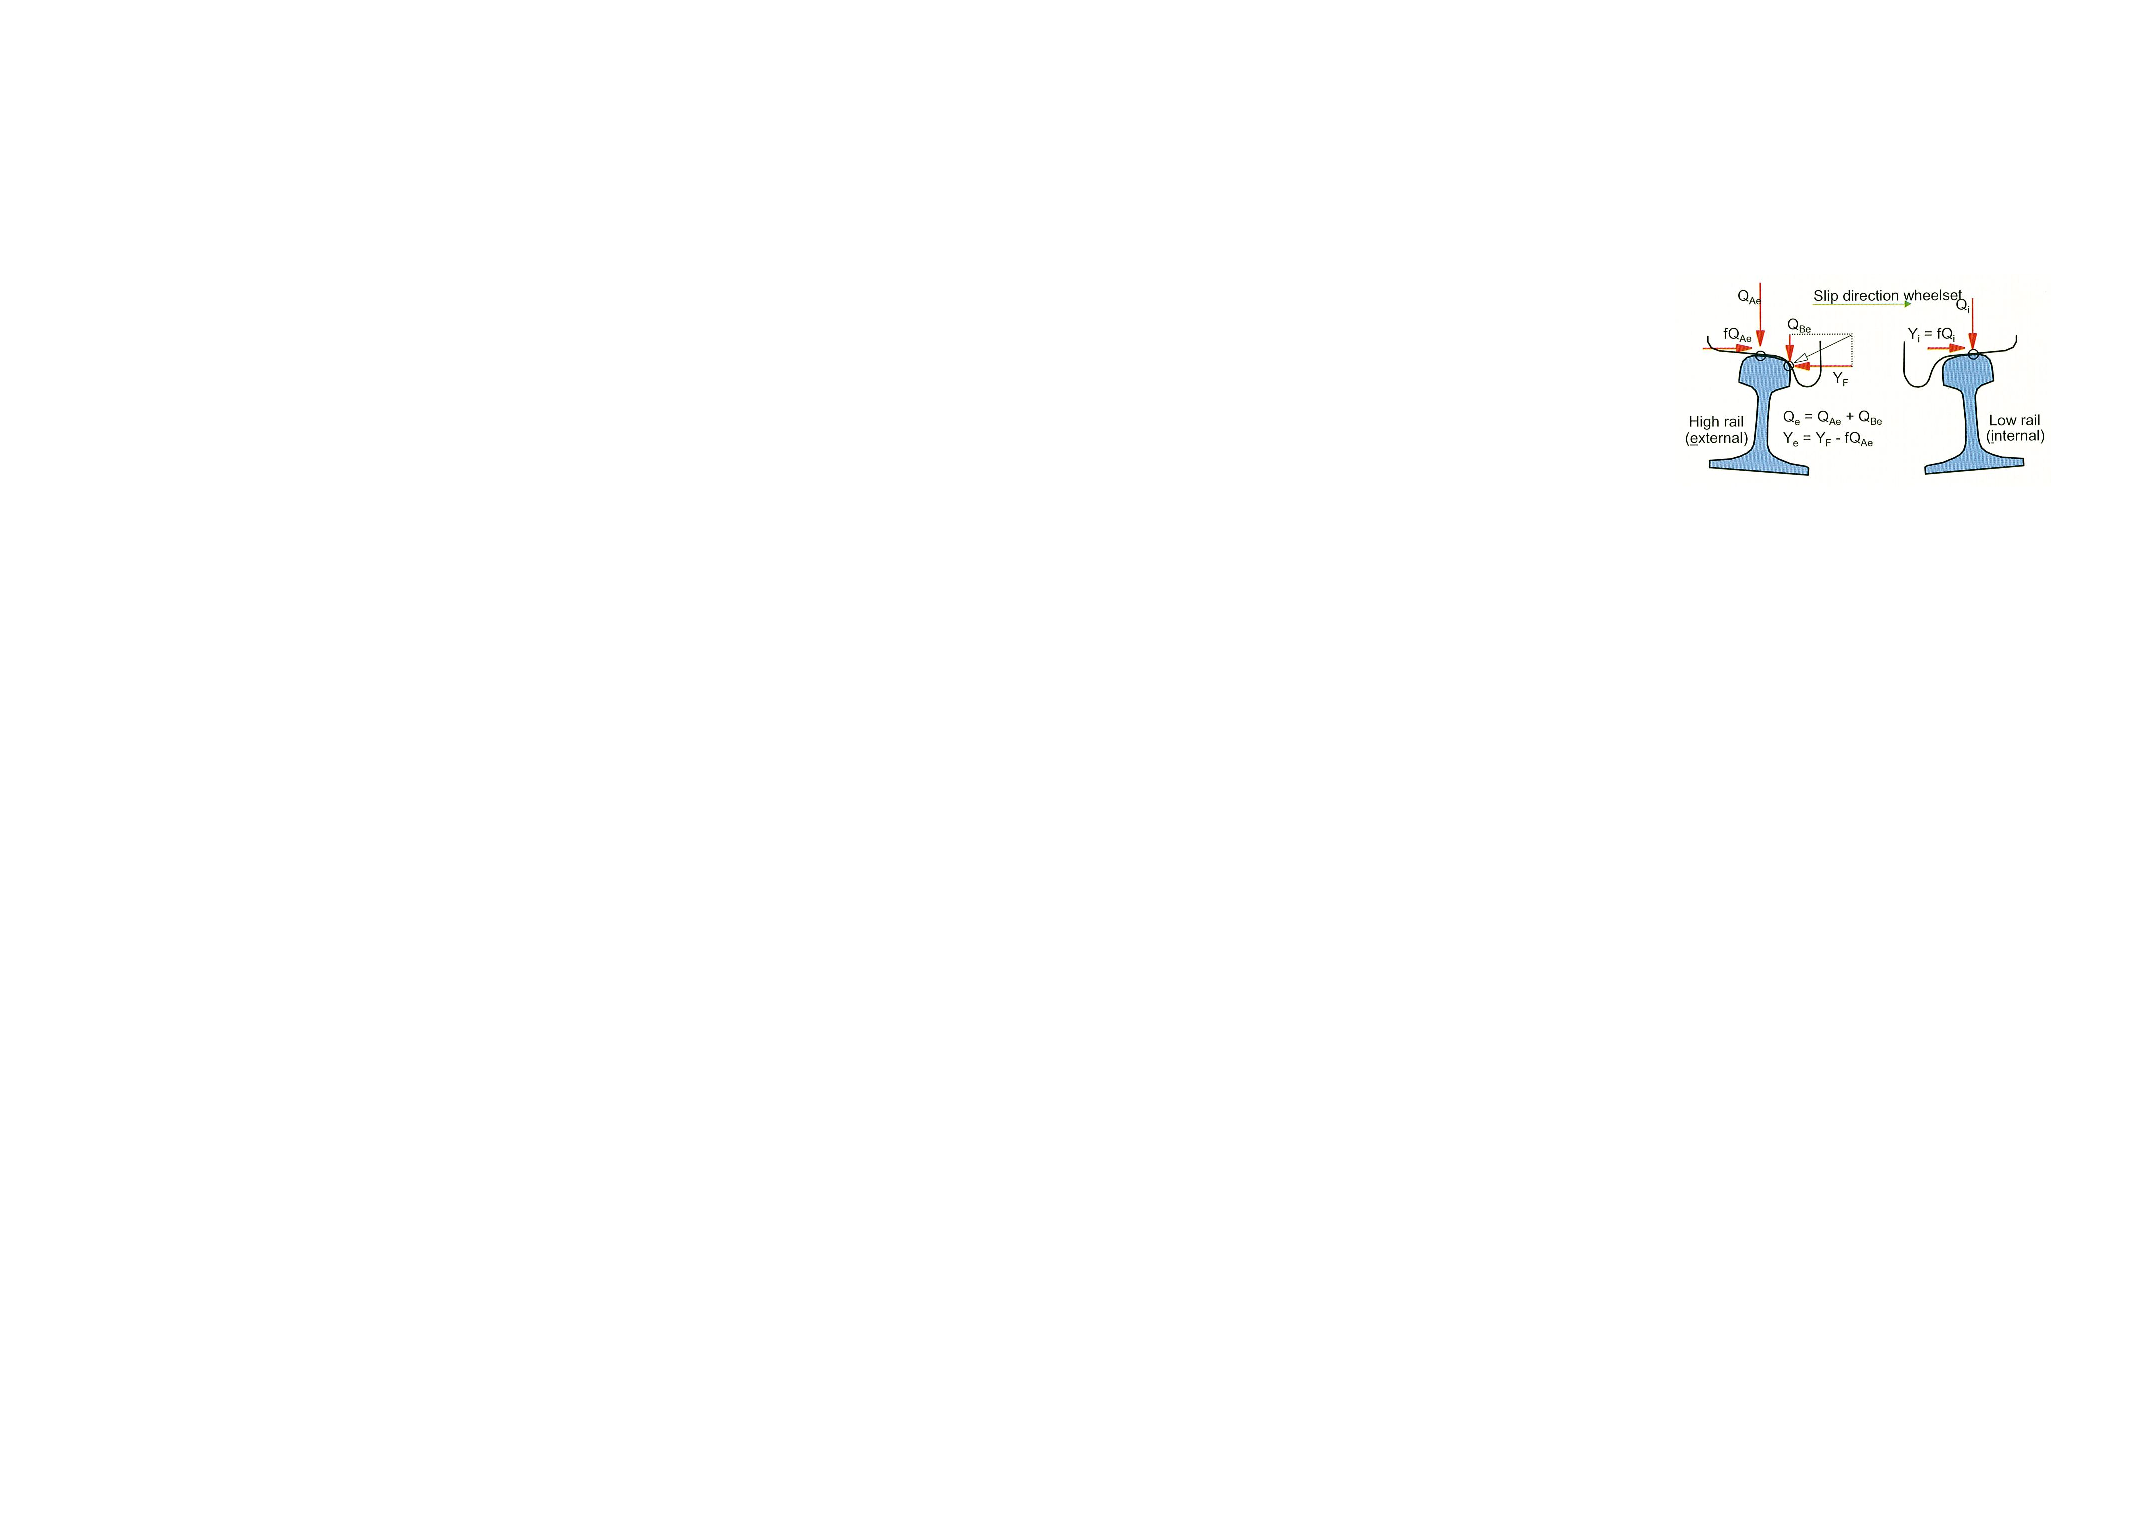
\includegraphics[width=\textwidth]{doublecontact}
%         \caption{Double contact point. Forces on rails in case of lateral slip in curves. Extracted from \citet[Figure 2.14]{esveld2001modern}}
%         \label{fig:doublecontract}
%     \end{subfigure}
%     \caption{Single and double contact of wheel-rail interface}
% \end{figure}
% \end{quote}
% \section{Wheel-Rail Interface}
% Following knowledge in all subsections of this section is extracted from \citet{esveld2001modern}. 
% \subsection{Wheelset and track dimensions}
% \begin{quote}
% Generally the track guage is used as a distance measured between the two rails, more specifically the distance between the inside of the railheads measured 14mm below the surface of the rail. By choosing 14 mm the measurement is less influenced by lipping or lateral wear on the rail head and by the radius r = 13 mm of the rail head face. On normal track the gauge is $1435^{+10}_{-3}$ mm with with a maximum gradient of 1:3000. For new track, however, NS apply the following standards:

% \begin{enumerate}
% \item Mean gauge per 200 m: $1435^{+10}_{-1}$ mm
% \item Standard deviation within a 200 m section less than 1 mm
% \end{enumerate}

% % \begin{figure}[h]
% % \centering
% % 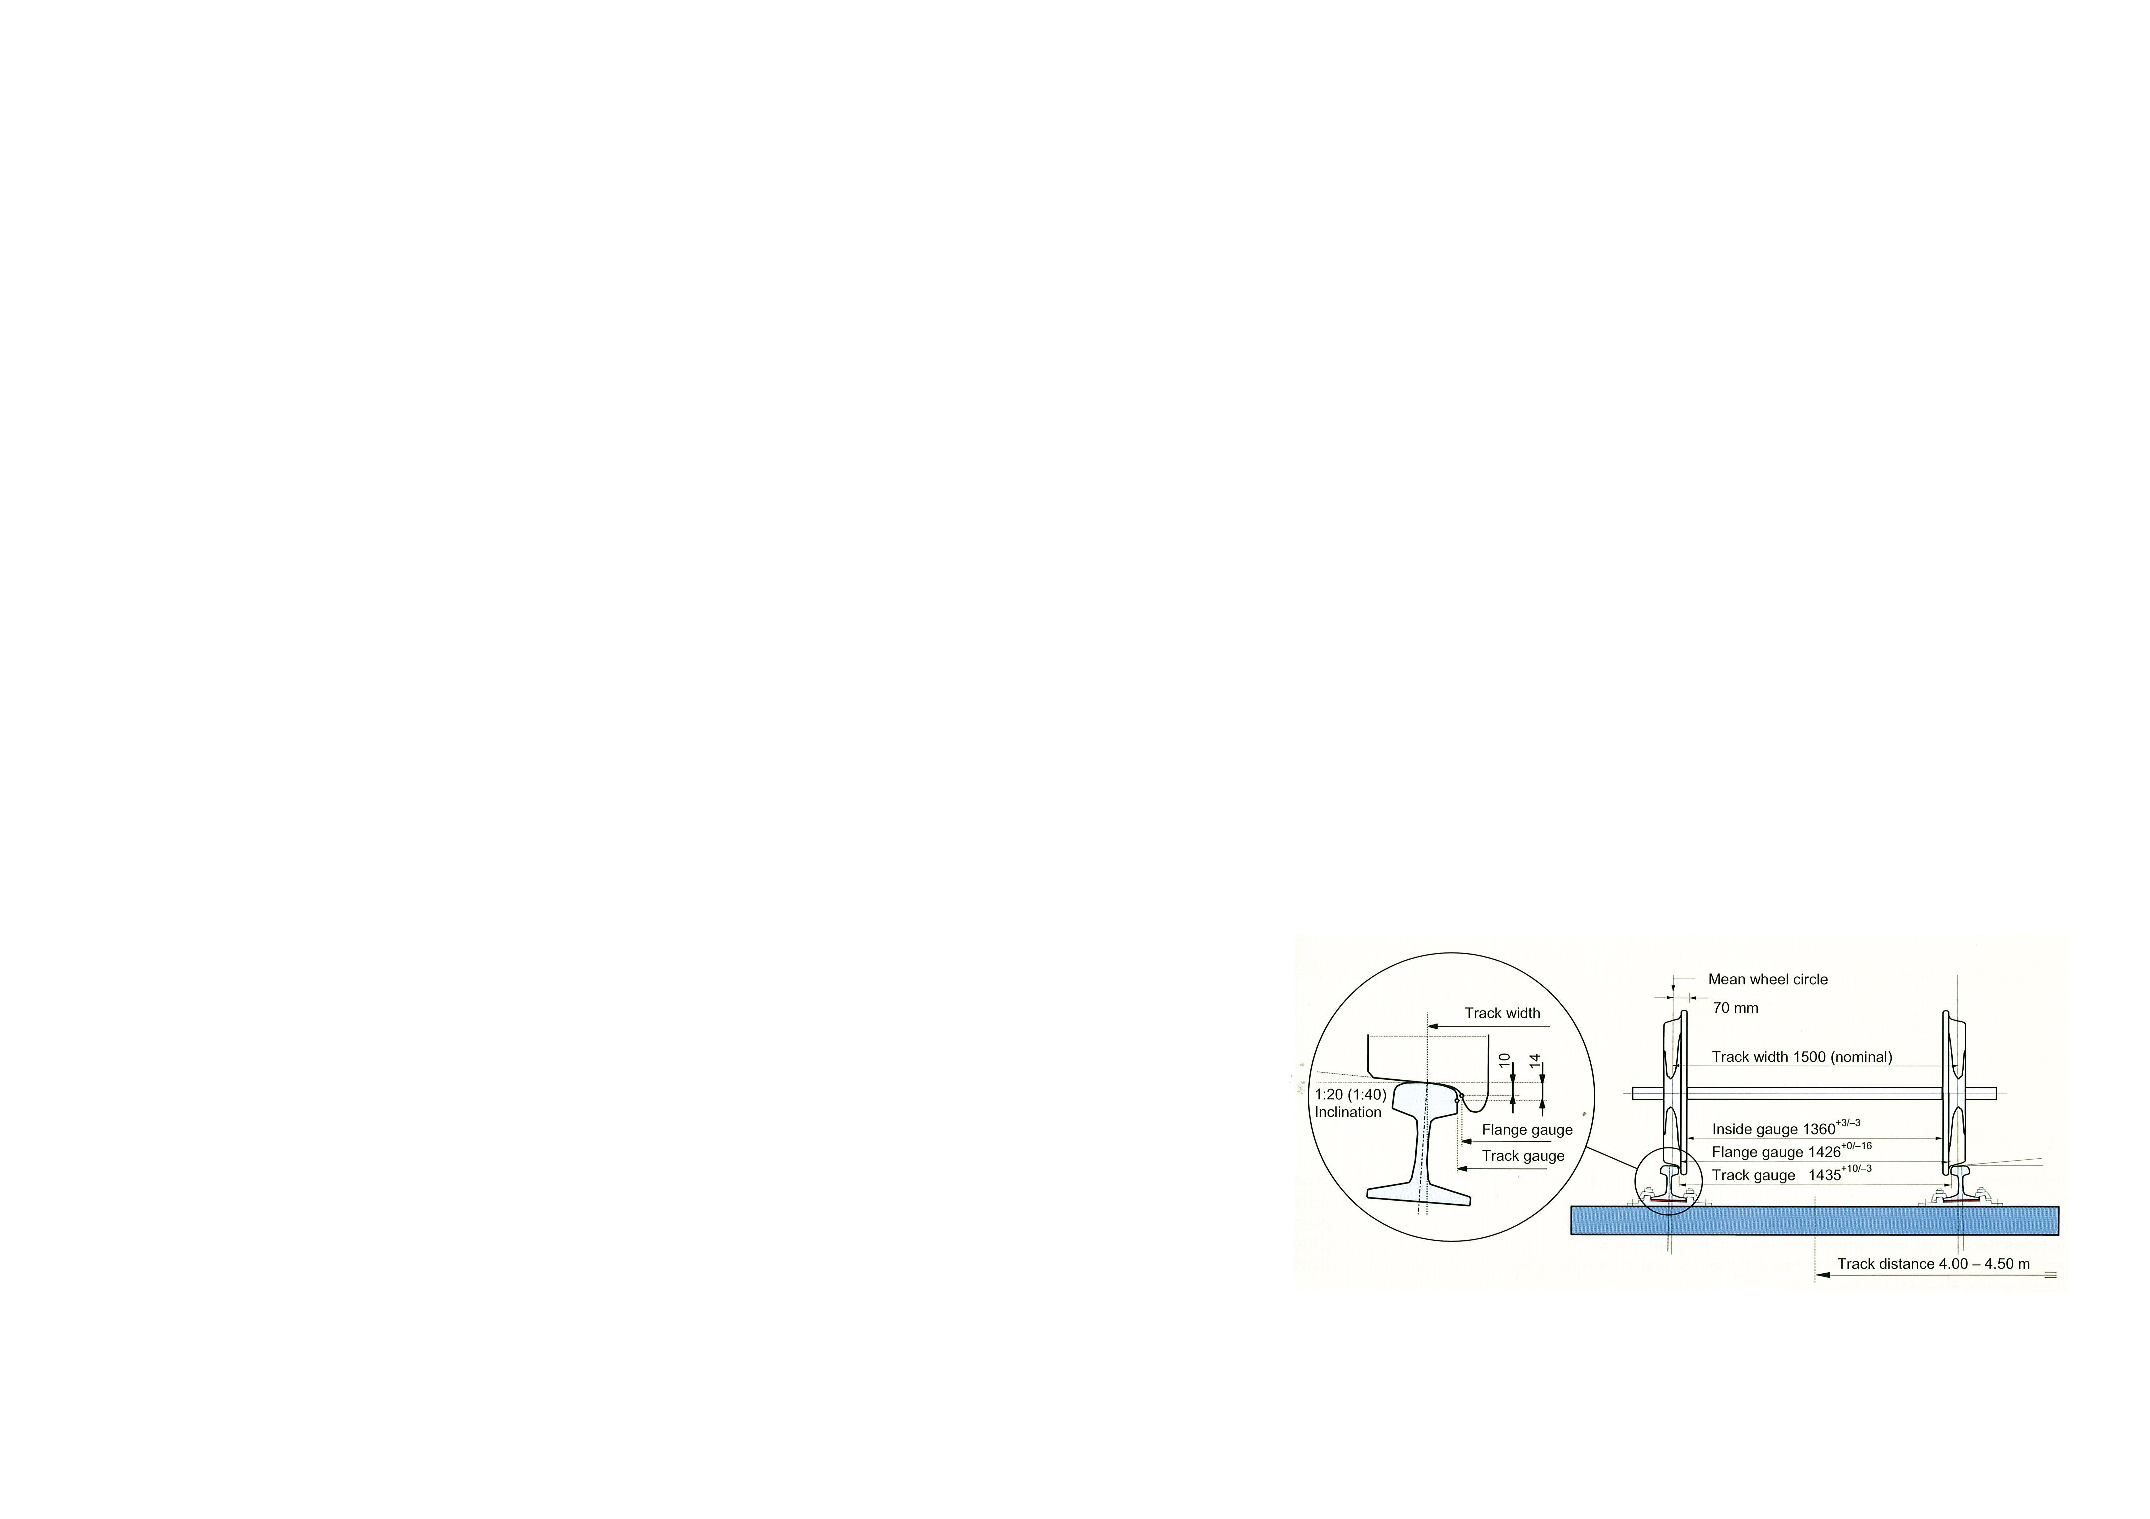
\includegraphics[width=0.8\textwidth]{wheelsettrackdimension.pdf}
% % \caption{Wheelset and track dimensions for straight normal gauge track. Extracted from \citet[p.17]{esveld2001modern}}
% % \label{fig:wheelset and track dimensions}
% % \end{figure}

% \end{quote}

% \subsection{Conicity and Equivalent Conicity of Wheels}

% \begin{quote}

% Originally conical tire profiles with an inclination of 1:20 were used. Since a centrally applied load on the railhead is desired, a rail inclination of 1:20, as shown in Figure 2.1, was also selected; this for instance still applies to NS profile NP 46. UIC 54 rail usually has an inclination of 1:40. This inclination matches the S 1002 worn wheel profile which is in general use in Europe. During manufacturing the tires are given a profile which matches the average shape cause by wear. In contrast to the straight conical profile this has a hollow form.

% It is clear that regarding a worn profile the conicity depends on the actual shape of the rail head and tire, including any wear, track gauge, and rail inclination. Likewise, elastic deformation of the wheelset and rail fastenings plays a role.

% Generally, the effective or equivalent conicity is defined as:

% $$ \gamma_e = \frac{\Delta r}{2y} = \frac{r_1 - r_2}{2y}  $$

% Here $r_1 - r_2$ is the instantaneous difference in rolling radius of the wheel treads; generally speaking this is a non-linear function of the lateral displacement y of the wheelset with respect to the central position. The difference between conical and worn profiles is given in Figure.\ref{fig:conicalwornprofiles}. To enable numerical comparisons $\gamma_e$ is determined at a certain lateral displacement $y=\bar{y}$.

% \end{quote}

% \subsection{Worn wheel profiles}

% \begin{quote}

% A perfectly conical wheel profile is unstable as far as its shape is concerned, but will take on a shape that is stable as the effect of wear.

% Practical research has shown that over a period of time wheel profiles stabilise with wear at an equivalent conicity of 0.2 to 0.3. With regards to running stability, the equivalent conicity must remain below 0.4 and to ensure the centering effect it must be greater than 0.1.

% \begin{figure}[h]
%     \centering
%     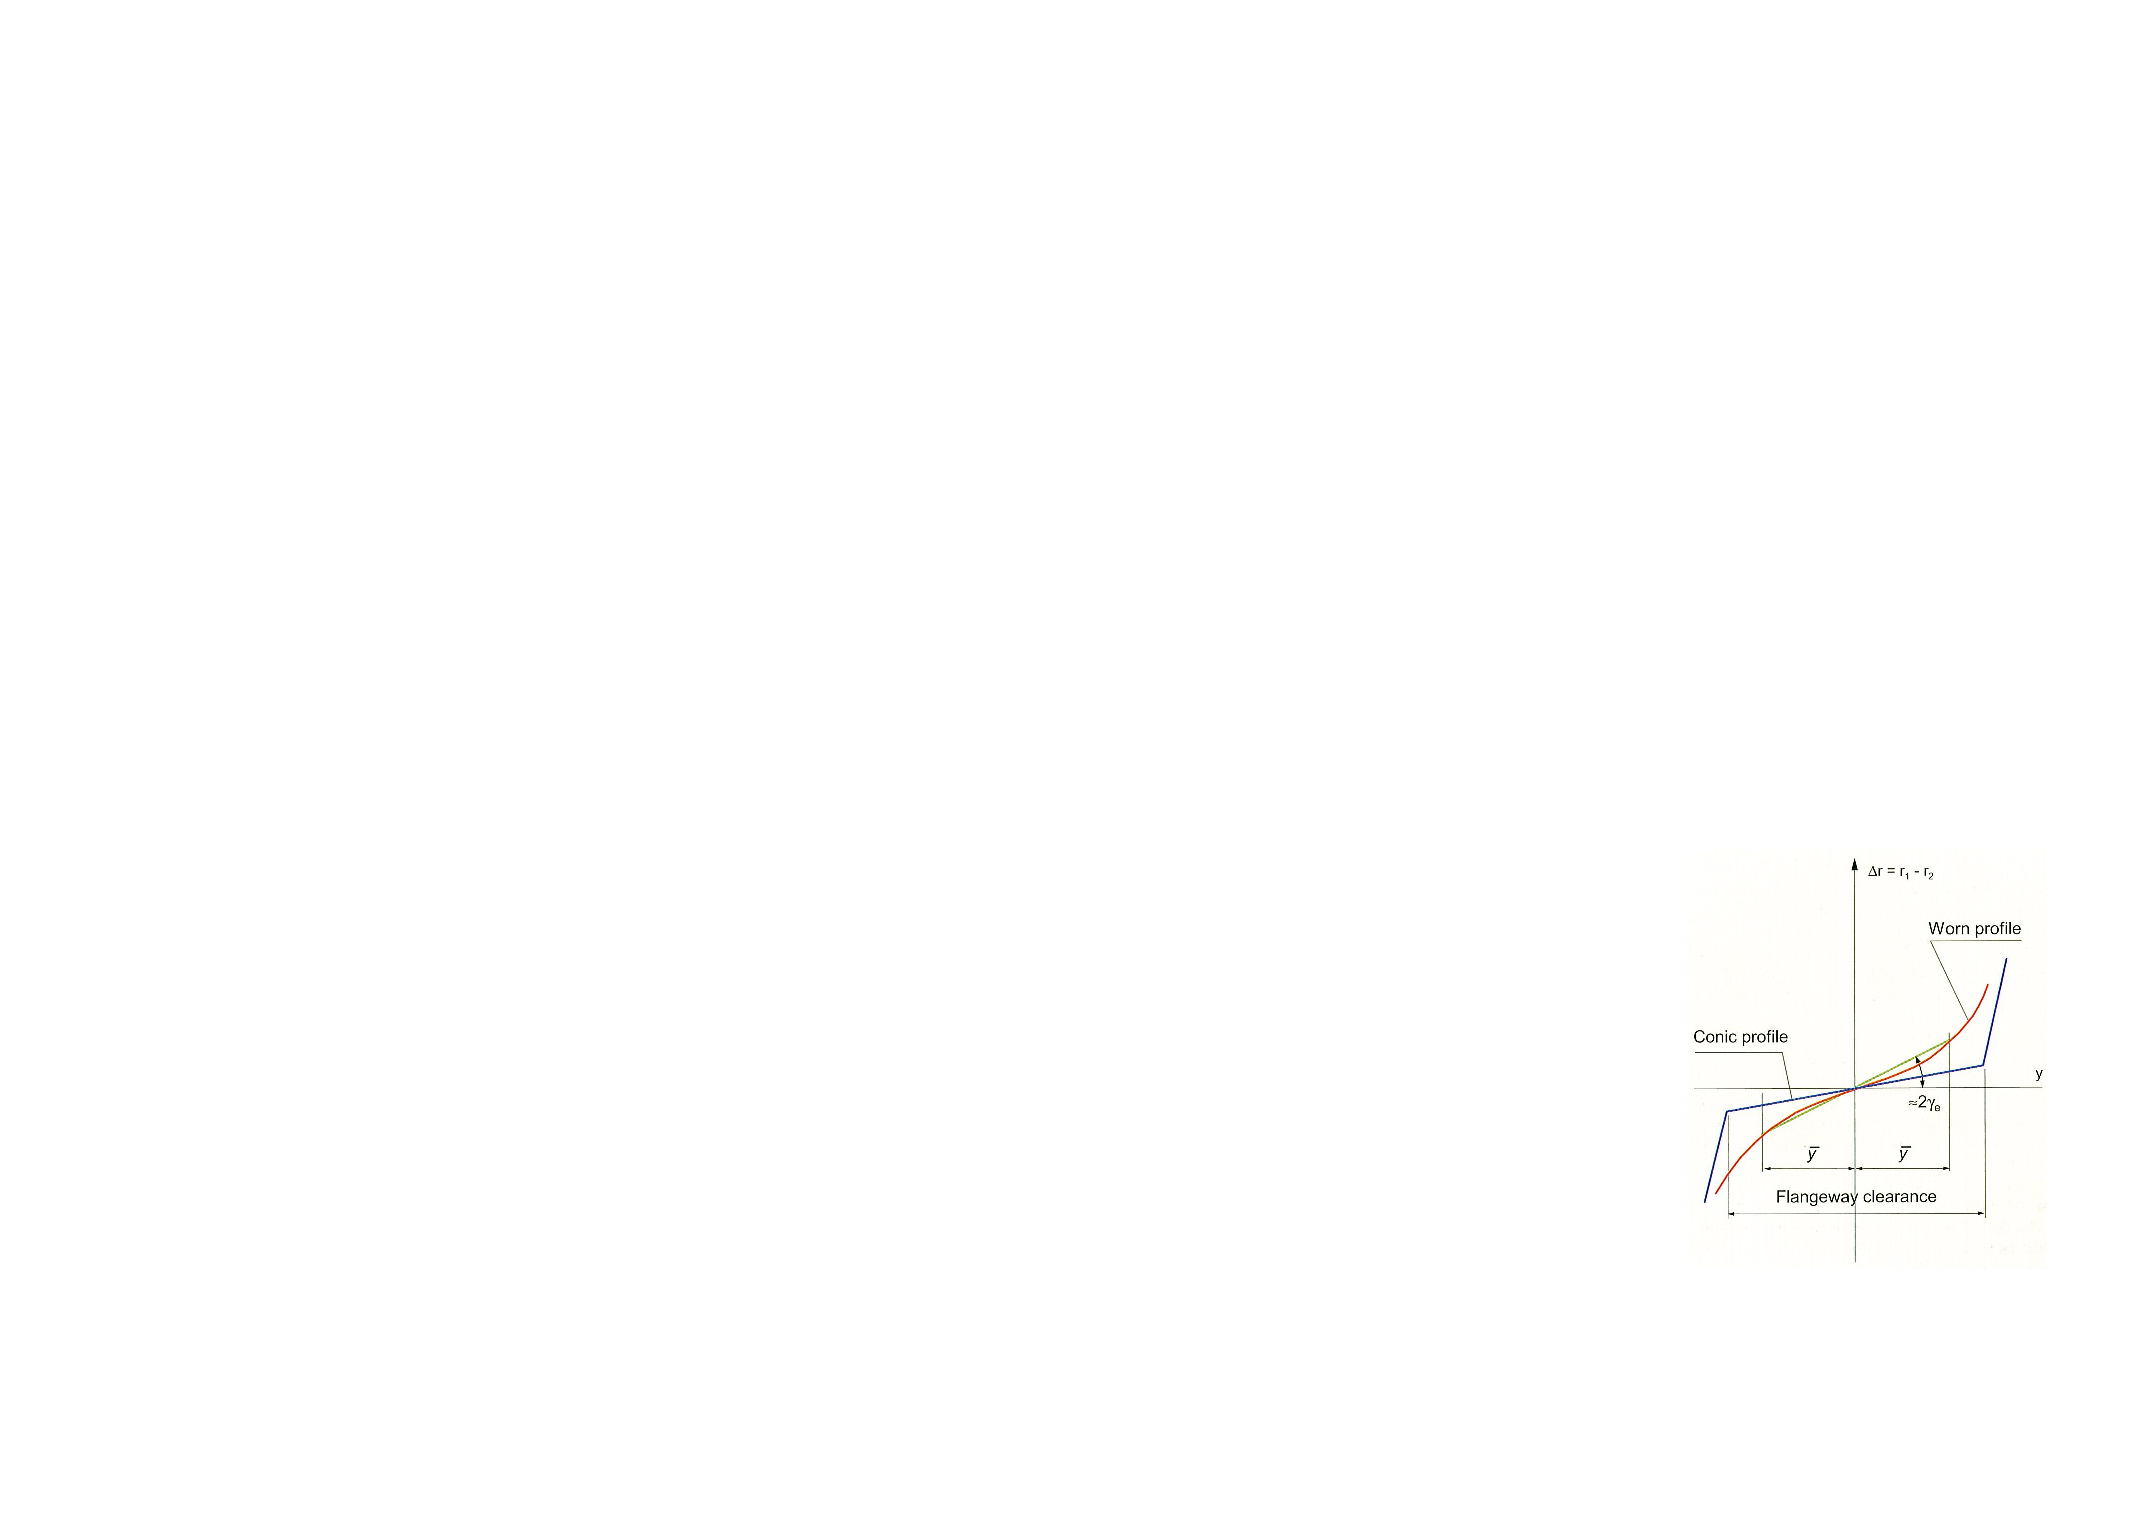
\includegraphics[width=0.6\textwidth]{conicalwornprofiles.pdf}
%     \caption{$y-\Delta r$ curves. Difference between conical and worn wheel profiles. Extracted from \citet[2.4]{esveld2001modern}}
%     \label{fig:conicalwornprofiles}
% \end{figure}

% With a conical profile the conicity is constant and above equation becomes:

% $$ \gamma_e = \frac{\Delta r}{2y} =\frac{(r+\gamma y)-(r-\gamma y)}{2y} = \gamma $$

% \end{quote}

% \section{Lateral Track Irregularities}\label{sec:lateraltrackirrgularities}

% This section describes allowable lateral track irregularities defined in EN13848-5\citet{13848}. 

% Lateral alignment irregularities was defined in EN13838-1. It states:"Deviation $y_p$ in y-direction of consecutive positions of point P... on any rail, expressed as an excursion from the mean horizontal position (reference line) covering the wavelength ranges stipulated below and calculated from successive measurements ...". See Figure \ref{fig:lateraldeviationdefine}.

% For lateral deviations, the following wavelengths shall be considered: $D1 = 3 -25 m$, $D2 = 25 - 70 m$ and $D3 = 70 - 200 m$. 

% \begin{figure}[h]
%     \centering
%     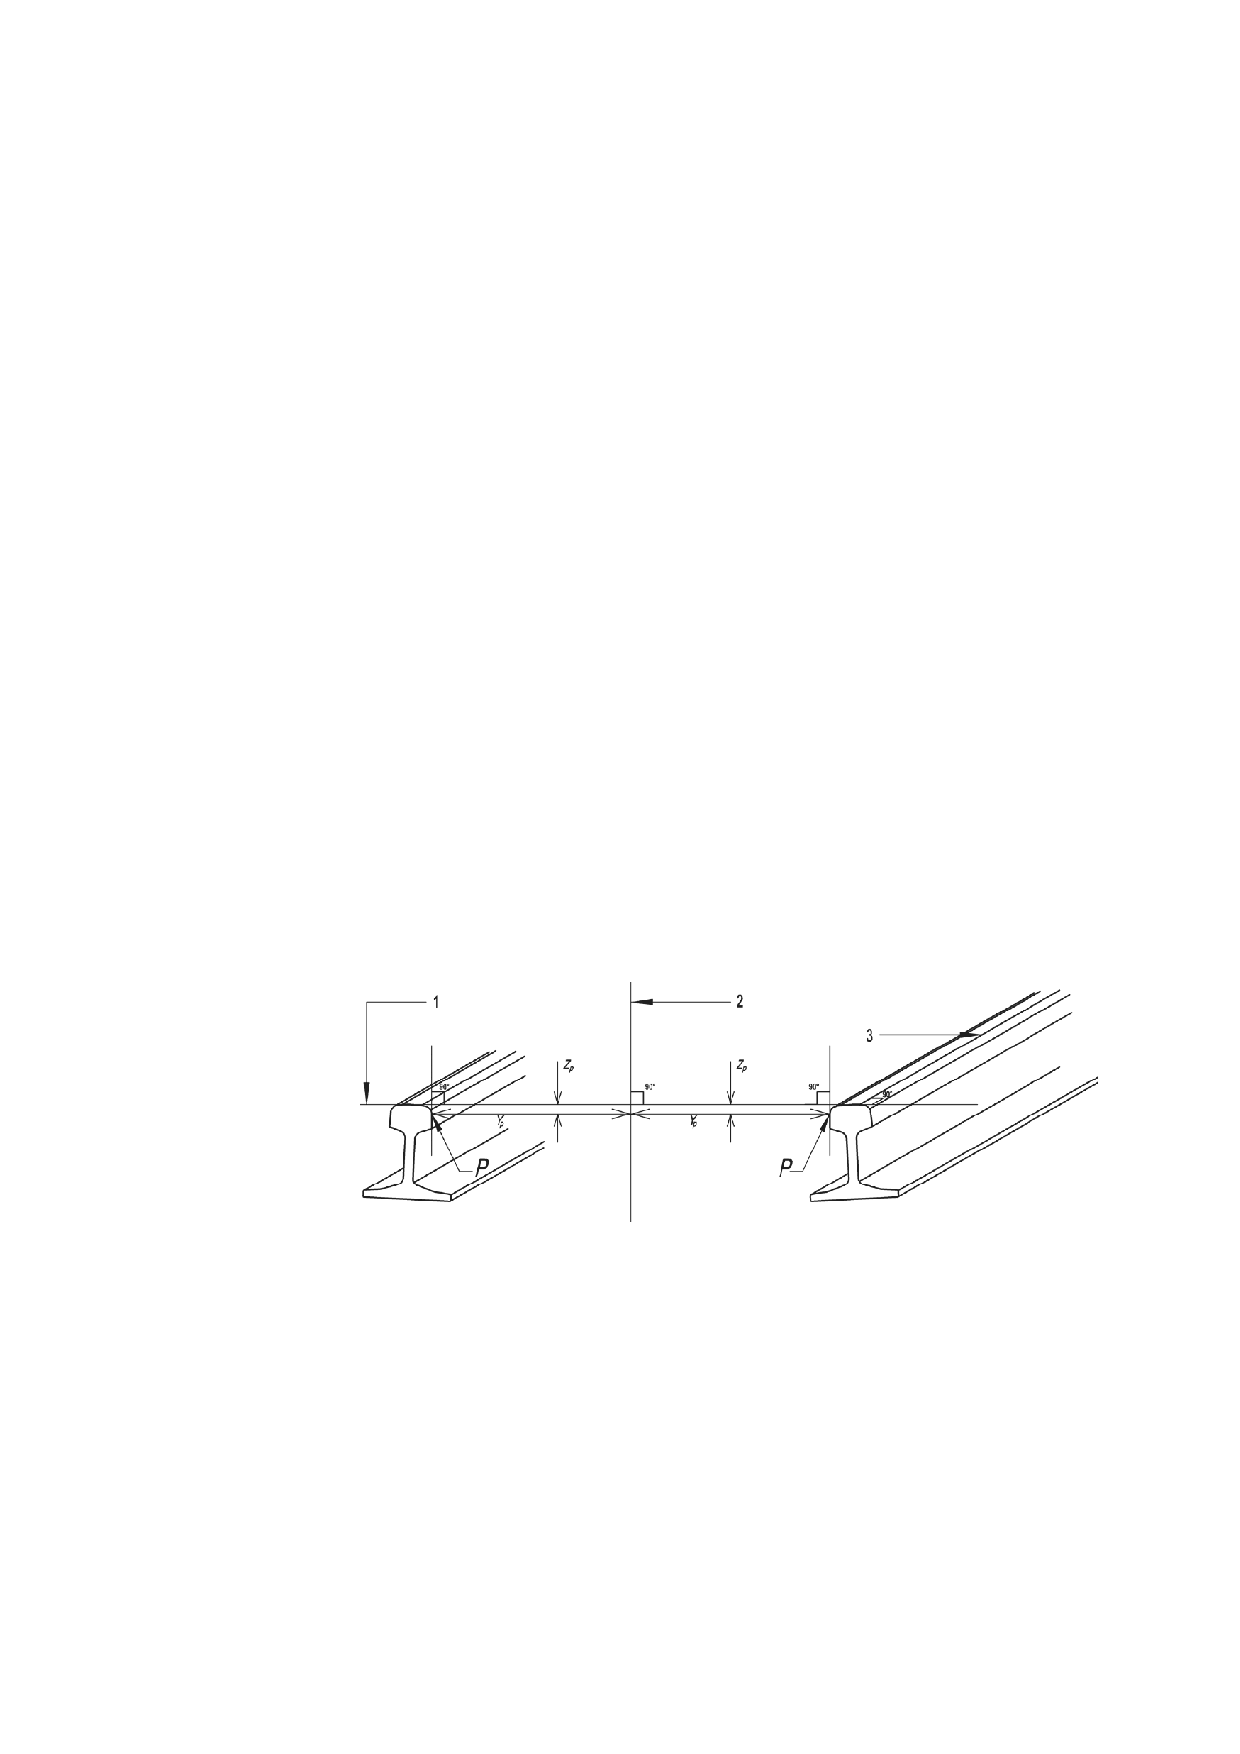
\includegraphics[width=0.8\textwidth]{lateraldeviationdefine}
%     \caption{Lateral deviation definition. Lateral deviations $y_p$ for each rail with 1: running surface, 2: reference line and 3: centre line of running table}
%     % \label{fig:lateraldeviationdefine}
% \end{figure}

% Table \ref{tab:lateraldeviation} defines the allowable standard deviation for lateral track irregularities. Lateral track irregularity has great influence on vehicle's lateral dynamic behaviour.

% \begin{table}[h]
%     \centering
%     \caption{Alignment - AL - Standard deviation. Extracted from \citet[Table B.6]{13848}}
%     \begin{tabular}{cc}
%         \hline
%         Speed(km/h) & Standard deviation(mm) \\
%         \hline
%         $V\leq 90$ & 1.5 to 1.8 \\
%         $80 < V \leq 120$ & 1.2 to 1.5 \\
%         $120 < V \leq 160$ & 1.0 to 1.3 \\
%         $160 <V \leq 230$ & 0.8 to 1.1 \\
%         $230 <V \leq 300$ & 0.7 to 1.0 \\
%         \hline
%     \end{tabular}
%     % \label{tab:lateraldeviation}
% \end{table}


% \section{Dynamic theories}

% \subsection{Natural frequencies and shapes of bridge}
% Undamped Euler-Bernoulli beam theory is adopted to obtain natural wave shapes and frequencies of a bridge structure. This theory is the simplest bridge dynamic model which assumes that the bridge behaves as a vibrating uniform beam. 

% The bridge is simply supported at both ends, and the stiffness is specified as a deflection at the mid span per unit span length arising from a static point load of 100kN at mid span.

% The equation of vibration of a uniform beam is:

% $$\frac{\partial^2 y}{\partial t^2} + a^2\frac{\partial^4 y}{\partial x^4}=0$$

% where: 

% y = deflection of beam

% x = coordinates along longitudinal axis

% t = time 

% $a^2$ = EI/m

% EI = flexural rigidity

% and, m = mass per unit length

% The general solution is:

% $$y(x,t) = (A\cos pt+B\sin pt)(C\cos kx + D\sin kx + F\cosh kx + Gsinh kx)$$

% which consists of independent time and distance parts. The distance dependent part of the solution gives the family of mode shapes which the beam will exhibit. Thus, generally, a beam has mode shapes which satisfy:

% $$y(x) = C\cos kx + D\sin kx + F\cosh kx + Gsinh kx $$

% For a beam which is simply supported at either end the general solution simplifies, giving a family of normalized amplitude mode shapes as follows:

% $$y_r = \sin \frac{r\pi x}{L}$$

% for $r = 1,2,3...,n$ and $L = span length$

% with corresponding angular frequencies, $\omega_r$, of:

% $$\omega_r = \frac{r^2 \pi^2}{L^2}\sqrt{\frac{EI}{m}}$$

% thus natural frequencies $f_r$ of beam, are:

% $$f_r = \frac{r^2 \pi}{2L^2}\sqrt{\frac{EI}{m}}$$

% \subsection{Basic resonance concept}
% The most simplest resonance scenario happens at a one degree-of-freedom mass-spring system loaded by a force whose frequency coincides with the natural frequency of mass-spring system.
% \begin{figure}[h]
% 	\centering
% 	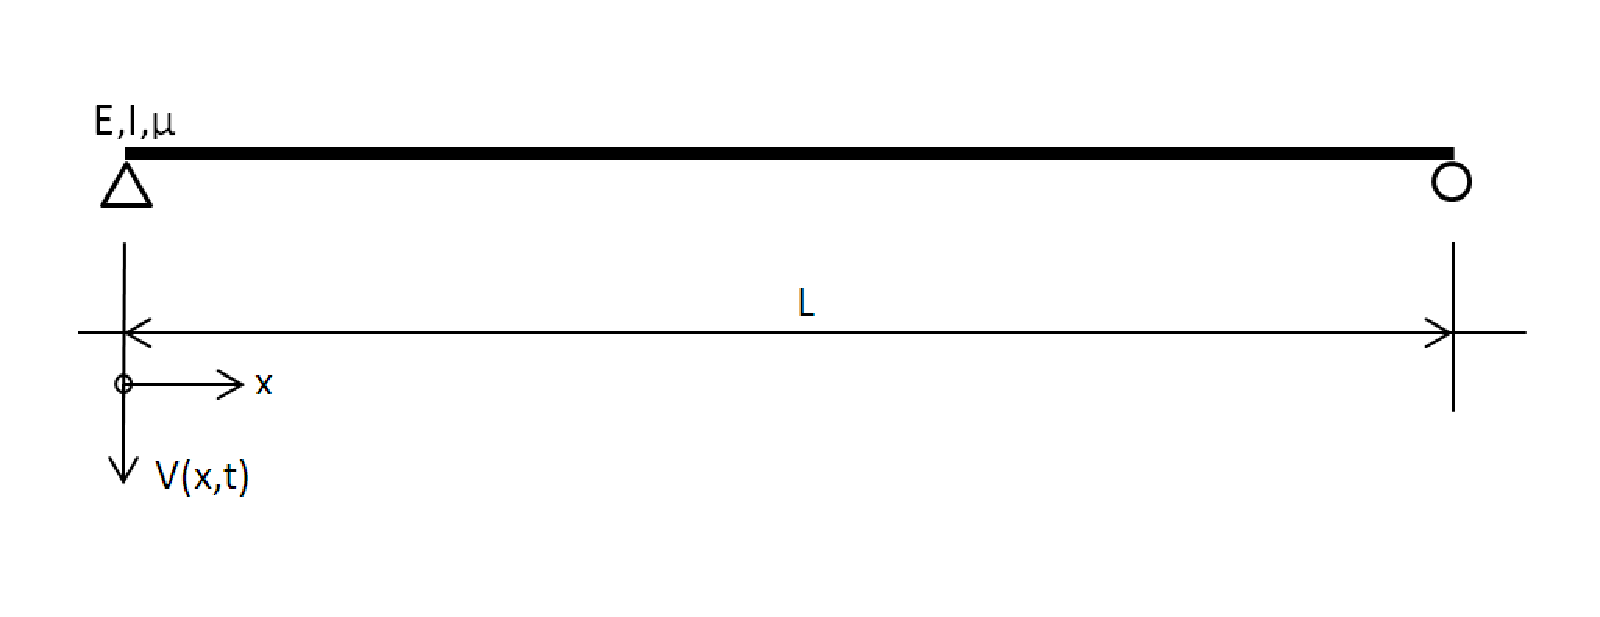
\includegraphics[width=0.8\textwidth]{massbeammodel.pdf}
% 	\caption{Mass beam model of span L}
% 	\label{fig:massbeammodel}
% \end{figure}

% Assume there is a simple one degree-of-freedom mass-spring system and an external force is acting on it. The force is given as $F(t)= F_0 \cos(\omega t)$. In this case the equation of motion takes the form
% \begin{equation}
% 	m\ddot{x} + kx = F_0 \cos(\omega t)
% \end{equation}

% The general solution can be written as
% \begin{equation}
% 	x(t) = A\cos(\omega_n t)+B\sin(\omega_n t) +\frac{F_0}{k}\frac{1}{1-\omega^2/\omega_n^2}\cos(\omega t)
% \end{equation}

% where $\omega_n = 2\pi\sqrt{k/m}$

% The unknown constants A and B depend on the initial conditions.

% The steady-state solution is given as:

% \begin{equation}
% 	x_{steady}= X \cos(\omega t) = \frac{F_0}{k}\frac{1}{1-\omega^2/\omega_n^2}\cos(\omega t)
% \end{equation}

% The amplitude of vibrations of the mass-spring system is given by:
% \begin{equation}
% 	|X|=|\frac{F_0}{k}\frac{1}{1-\omega^2/\omega_n^2}|
% \end{equation}

% The amplitude-frequency dependencies is shown in \ref{fig:amplitude-frequency-characteristic} 

% \begin{figure}[h]
% 	\centering
% 	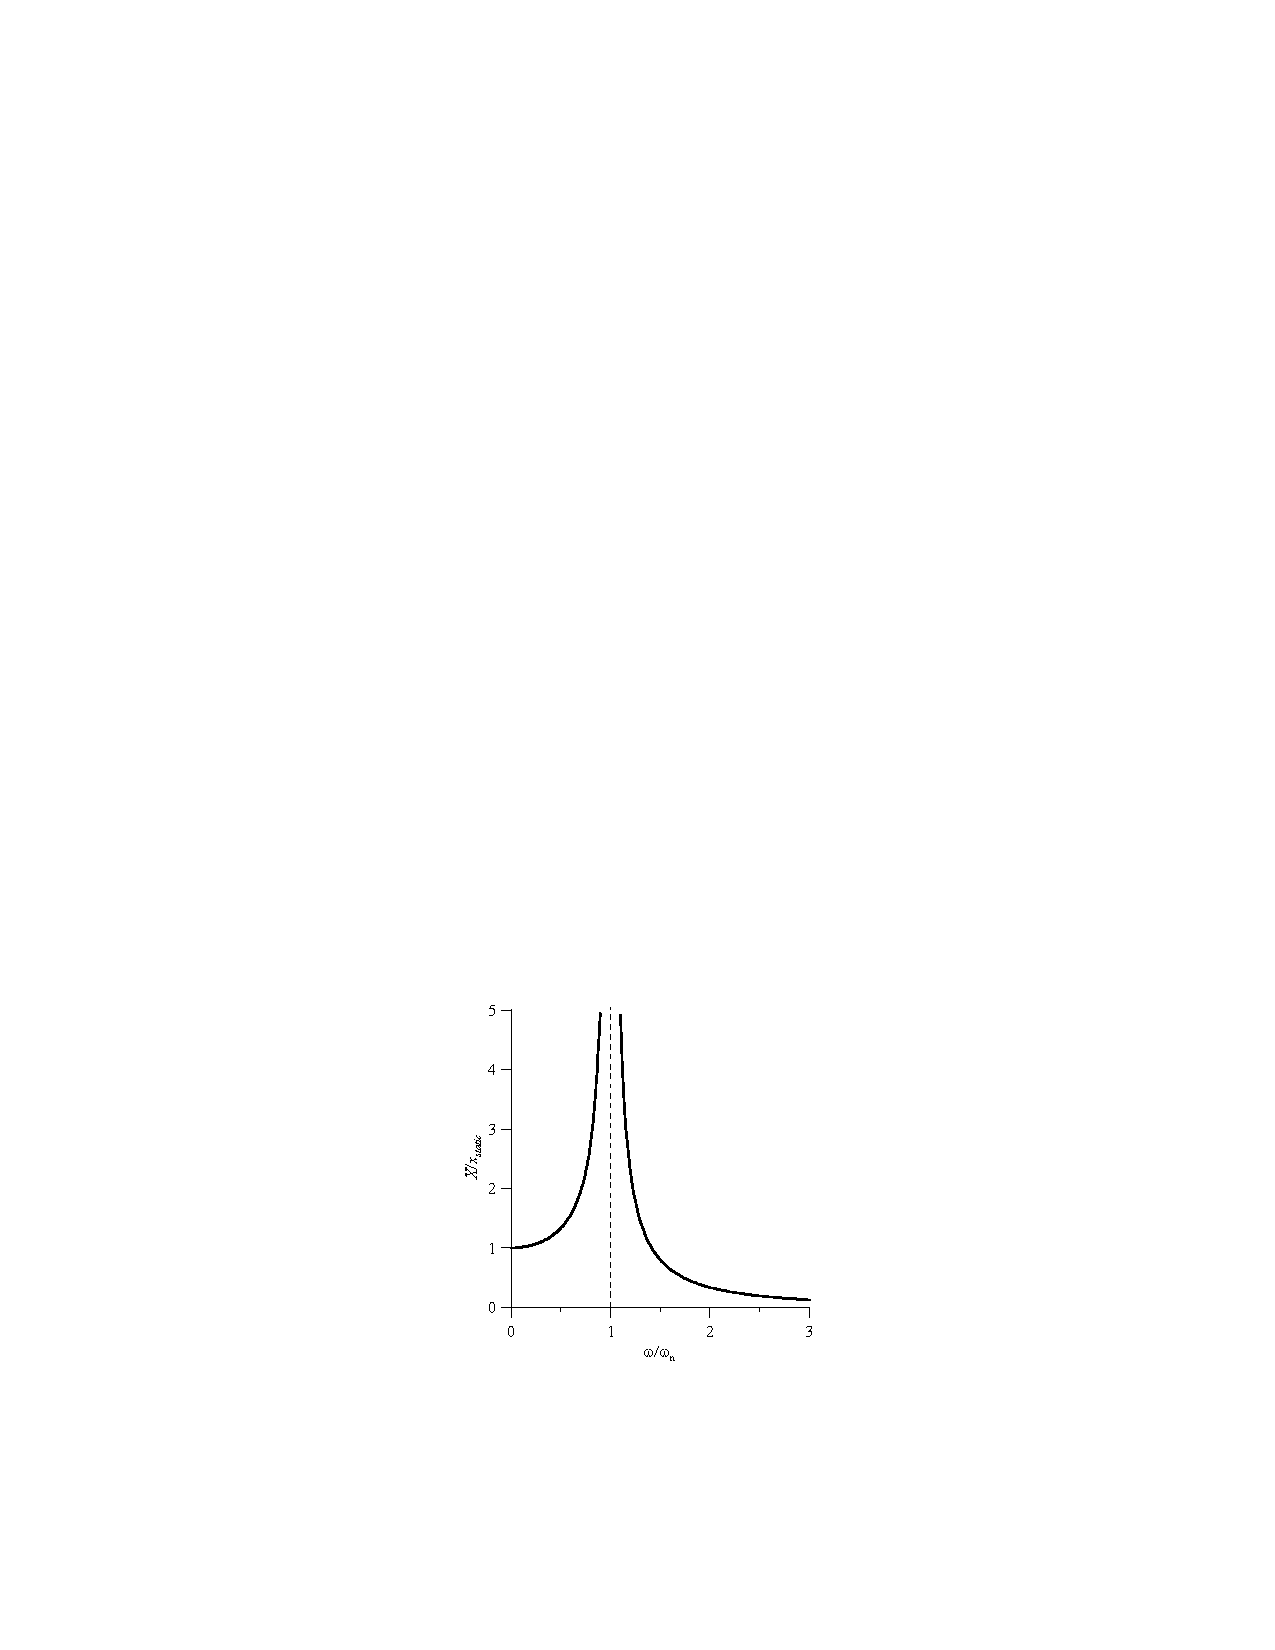
\includegraphics[width=0.6\textwidth]{amplitudefrequencycharacteristic.pdf}
% 	\caption{Amplitude-frequency characteristic. Extracted from \citet[2.2.2]{dynamicslecturenote}}
% 	\label{fig:amplitude-frequency-characteristic}
% \end{figure}

% When the frequency of force equals frequency of mass-spring system, the amplitude of vibration is infinitely high. It means system becomes unstable and normally it's a dangerous sign. This phenomenon is called resonance.

% Resonance can also happen when a harmonic force is loaded on an Euler-Bernoulli beam. It can be loaded anywhere on the beam to produce resonance. 


% \section{Analysing methods for lateral dynamics of railway bridges }

% Several analysing methods for vertical dynamics of railway bridges were briefed in \citet[A6.2]{UIC776-2}. Methods that can be applied also on lateral direction are selected:

% \begin{quote}

% Various programs are available and details can be found in ERRI report D 214/RP7 (see Bibliography - page 43); they can be used to calculate the dynamic response under live train loads, of isostatic bridges, series of isostatic decks, continuous bridges using the beam theory, the dynamic response of plates and by taking into account the two longitudinal and transversal modes. They can also run calculations for orthotropic square plates and skew plates.

% ...

% Two types of analyses can be carried out: with or without interaction with the train.

% The most problematic cases, for example special structures (bridges with long spans such as bowstring bridges), have to be solved using generic finite element programs.

% Various programs such as ANSYS, NASTRAN, ABAQUS, SAP, FASTRUDL and so on, can be used to obtain the modal responses of bridge decks. Modelling can be done with beam models using torsional characteristics if the bridge is not a skew bridge and the structure is not a special case (see above). However, spatial modelling is necessary in such cases.

% Dynamic analysis of a structure can be used to resolve a system of differential equations of lesser importance. Two fundamental approaches may be implemented: one method consists in solving the system of equation by direct integration, whereas the other defines the solution based on the natural modes of vibration of the structure. This is known as modal superposition. 
% \end{quote}

% \subsection{Modal analysis}

% Knowledge on modal analysis is extracted from \citet{UIC776-2}

% \begin{quote}

% Modal analysis is used to calculate the natural modes and frequencies of the model, as well as resulting variables(participation factors, effective modal masses)

% For undamped, free vibrations, the equation of movement without a second element is reduced to:

% $$  [K] - \omega^2[M][\Phi_i] = 0 $$

% where $\Phi$ represents the circular frequency vector (=pulse) and $[\Phi]$ is the modal crossing matrix consisting of natural orthonorm modal vectors $[\Phi_i]$ in relation to $[M]$ or $[K]$.

% In principle, all the modes with natural frequencies lower than the cut-off frequency should be retained; in practice, the modes retained are often those making an important contribution to the response(criterion of the sum of effective modal mass of the structure). When the natural vectors are calculated, the modal matrix is formed $[\Phi]$ after which the $\omega_i$ can be deduced.

% \end{quote}

% \subsection{Analysis by modal superposition}

% Knowledge on modal superposition is extracted from \citet{UIC776-2}

% \begin{quote}
% The fundamental equation of the dynamic approach represents a system of N simultaneous differential equations, where N is the number of degrees of freedom of the structure. If three-dimensional modelling is used, this number N is equal to six times the number of nodes less the number of ddl blocked at the supprt. When the number increases to a value that is very high for large models, the size of the problem needs to be reduced by transformation techniques. Solving the differential equations then becomes faster and is more accurate.

% The integration method used is now as follows: for each mode i, the resulting equation gives an evaluation introduced by the Duhamel integral of the Fourier transform. The sum of the solutions gives the full response. The integration approach for mobile loads is a slow process.

% Modal superposition is used to accurately quantify the respective contributions of each mode to the total dynamic response and to identify the risks of resonance and dynamic amplification of some types of stresses.
% \end{quote}

% \subsection{Numerical methods}

% Knowledge on numerical methods is extracted from \citet{UIC776-2}

% \begin{quote}

% When the analysis uses numerical methods to directly integrate the dynamic equation, the loads become the dynamic system in the case of vehicles and their internal behaviour impacts the response from the structure.

% - the two systems can be considered separate systems,

% - the vehicle can be considered a finite element.

% This last method takes track profile defects into account and deduces the force of interaction between the structure and the vehicle as well as the internal forces in the dynamic system that is built.

% In this method, the equation of the dynamics is solved, with or without prior transformation, by using the conventional algorithms for numerical resolution of second-degree differential equations. These numerical methods calculates the response to regularly spaced time intervals(in general). The selected time pitch determines the accuracy of the results and has a bearing on the length of computer calculations.

% Numerical integration methods are all based on the search for balanced solutions of the dynamic equation at regular time intervals.

% \end{quote}

% \subsubsection{VAMPIRE}

% VAMPIRE is a FEM simulation software developed by DeltaRail. It allows the user to build a dynamic model of any rail vehicle and study the response of the vehicle to real measured track geometry or user specified inputs in the form of track displacements and external force inputs. Rail vehicles can be modelled with simulated instrumentation allowing almost any aspect of behaviour to be studied. 

% \begin{figure}[h!]
%     \centering
%     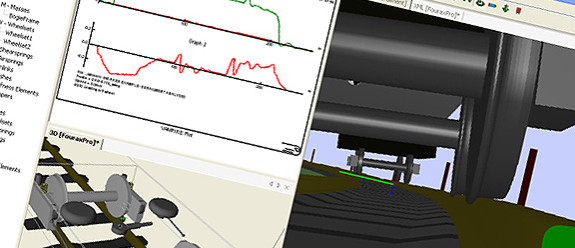
\includegraphics[width=0.8\textwidth]{vampire}
%     \caption{A sample project being conducted in VAMPIRE}
%     \label{fig:vampire}
% \end{figure}

% There are also many similar simulation software on the market which puts emphasis on railway vehicle dynamic behaviour, but VAMPIRE is specially selected for introduction because it was the software used by D181 committee, whose report series originally proposed 1.2Hz criterion by using the assistance of VAMPIRE. Also, the output results provided by D181 reports is an important foundation for the development of new practical method. More detailed description of these VAMPIRE simulation runs will be illustrated in Chapter.\ref{sec:D181reportseries}.

\chapter{Literature Review of regulations regarding lateral railway bridge dynamics in 1991-2} 
Eurocode 1990 and Eurocode 1991-2 and their corresponding National Annex are primary codes to be fulfilled through out the whole process of conducting a railway bridge in Netherlands. It is of great importance to study dynamic effect on railway bridges due to increasing usage of public train service.

This literature review aims to filter out criteria and requirements related to lateral railway bridge dynamics in EN1991-2.


\section{Factors influencing dynamic behaviour}
As stated in\citet[6.4.2]{EC12} there are 11 factors influencing dynamic behaviour of a railway bridge. The principal factors which influence dynamic behaviour are:
\begin{enumerate}[-]
	\item the speed of traffic across the bridge
	\item the span L of the element and the influence line length for deflection of the element being considered
	\item the mass of the structure
	\item the natural frequencies of the whole structure and relevant elements of the structure and the associated mode shapes (eigenforms) along the line of the track
	\item the number of axles, axle loads and the spacing of axles
	\item the damping of the structure
	\item vertical irregularities in the track
	\item the unsprung/sprung mass and suspension characteristics of the vehicle
	\item the presence of regularly spaced supports of the deck slab and/or track (cross girders, sleepers etc.)
	\item vehicle imperfections (wheel flats, out of round wheels, suspension defects etc.)
	\item the dynamic characteristics of the track (ballast, sleepers, track components etc.)
\end{enumerate}

\vspace*{0.2cm}

Other factors may include:

\begin{enumerate}

	\item The track number of the bridge and their alignment. 
	\item Multiple trains running on bridge simultaneously. 
	\item Track alignment

\end{enumerate}

\section{Requirements for railway bridge verification}
\citet{EC0} propose following requirements. Criteria regarding lateral direction are bolded.


\begin{enumerate}
	\item Checks on bridge deformations shall be performed for traffic safety purposes for the following items:
	\begin{enumerate}[-]
		\item vertical accelerations of the deck
		\item vertical deflection of the deck throughout each span
		\item unrestrained uplift at the bearings(to avoid premature bearing failure)
		\item vertical deflection of the end of the deck beyond bearings(to avoid destabilising the track, limit uplift forces on rail fastening systems and limit additional rail stresses) 
		\item twist of the deck measured along the centre line of each track on the approaches to a bridge and across a bridge(to minimise the risk of train derailment)
		\item rotation of the ends of each deck about a transverse axis or the relative total rotation between adjacent deck ends(to limit additional rail stresses, limit uplift forces on rail fastening systems and limit angular discontinuity at expansion devices and switch blades)
		\item longitudinal displacement of the end of the upper surface of the deck due to longitudinal displacement and rotation of the deck end(to limit additional rail stresses and minimise disturbance to track ballast and adjacent track formation)
		\item \textbf{horizontal transverse deflection(to ensure acceptable horizontal track radii)}
		\item \textbf{horizontal rotation of a deck about a vertical axis at ends of a deck (to ensure acceptable horizontal track geometry and passenger comfort)}
		\item \textbf{limits on the first natural frequency of lateral vibration of the span to avoid the occurrence of resonance between the lateral motion of vehicles on their suspension and the bridge}
	\end{enumerate}
	\item Checks on bridge deformations should be performed for passenger comfort, i.e. vertical deflection of the deck to limit coach body acceleration in accordance with A2.4.4.3\citet{EC0}
	\item The limits given in A2.4.4.2 and A2.4.4.3\citet{EC0} take into account the mitigating effects of track maintenance (for example to overcome the effects of the settlement of foundations, creep, etc.) 
\end{enumerate}


\section{Horizontal transverse dynamic effects}
There's only one criterion in the Eurocodes mentiones that the bridge's first lateral natural frequency should not be lower that 1.2 Hz. 

However, as more and more long-span bridges are built nowadays, this requirement is not valid for more bridges. This is because, in general, the lateral natural frequency of a bridge decreases when span increases. For bridges with span longer than 150m, there's few bridge can have a lateral frequency higher than 1.2Hz, according to senior engineers' designing experience.

So it is vital to discuss horizontal dynamic effects for the sake of longer span bridges. In addition, a study has been carried out on the requirements for horizontal vibration of railway bridges to make the results of dynamic analysis usable.



\subsection{Nosing force}\label{sec:nosingforce}
Nosing force is defined in Eurocode 1991-2. Its original background can be found in \citet[Proposed criteria]{d181}. It is defined as a representation of actions, in combine with actions like vertical loads, dynamic effects, centrifugal forces, traction and braking forces, etc.

The evidence of RP6 is the background of nosing force in EN1991-2 is the following repeating literature:

In \citet[6.5.2]{EC12}:
\begin{quote}
	(1)P The nosing force shall be taken as a concentrated force acting horizontally, at the top of the rails, perpendicular to the centre-line of track. It shall be applied on both straight track....
\end{quote}

In \citet[4.1B]{d181}:
\begin{quote}
	These forces shall be applied at the top of the rails in the most unfavourable position and acting horizontally, perpendicular to the track centreline...
\end{quote}

With another statement also helps proofing RP6 is the background of nosing force in EN1991-2 in \citet[4:Draft Recommendations]{d181}:

\begin{quote}
	These can therefore be expressed as follows: (Article \textbf{6.5.2} of ENV 1991-3 of 1994)...
\end{quote}

ENV 1991-3 was renamed to EN 1991-2 in 2003.

Originally in \citet[4:Draft Recommendations]{d181}, nosing forces was defined as lateral forces from vehicle/bridge interaction as a result of \textbf{hunting}.

The characteristic value of the nosing force shall be taken as $Q_{sk} = 100kN$. It shall not be multiplied by the factor $\Phi$ (\citet[6.45]{EC12}) or by the factor $f$ in \citet[6.51]{EC12}. 

The characteristic value of the nosing force should be multiplied by the factor $\alpha$ in accordance with \citet[6.3.2]{EC12} for values of $\alpha \geq 1$

The nosing force shall always be combined with a vertical traffic load.



\subsection{Verification of the Limit States}
\citet[6.4.6.5]{EC12} proposes following principles to be followed during design:

To ensure traffic safety:
\begin{enumerate}
	\item The verification of maximum peak deck acceleration shall be regarded as a traffic safety requirement checked at the serviceability limit state for the prevention of track instability
	\item The dynamic enhancement of load effects shall be allowed for by multiplying the static loading by the dynamic factor $\varPhi$ defined in \citet[6.4.5]{EC12}. If a dynamic analysis is necessary, the results of the dynamic analysis shall be compared with the results of the static analysis enhanced by $\varPhi$ (and if required multiplied by $\alpha$ in accordance with \citet[6.3.2]{EC12}) and the most unfavourable load effects shall be used for the bridge design.
	\item If a dynamic analysis is necessary, a check shall be carried out according to \citet[6.4.6.6]{EC12} to establish whether the additional fatigue loading at high speeds and at resonance is covered by consideration of the stresses due to load effects from $\varPhi \times LM71$ (and if required $\varPhi \times Load Model SW/0$ for continuous structures and classified vertical load in accordance with \citet[6.3.2(3)]{EC12} where required). The most adverse fatigue loading shall be used in the design.  
\end{enumerate}

\subsection{Serviceability limit states - traffic safety}


\subsubsection{Transverse deformations and vibrations}\label{sec:Transverse-deformations-and-vibrations}
\citet[A2.4.4.2.4]{1990a2}  proposed that transverse deformation and vibration of the deck shall be checked for characteristic combinations of Load Model 71 and SW/0 as appropriate multiplied by the dynamic factor $\phi$ and $\alpha$ (or real train with the relevant dynamic factor if appropriate), wind loads, nosing force, centrifugal forces in accordance with \citet[6]{EC12} and the effect of a transverse temperature differential across the bridge.

The transverse deflection $ \delta_h $ at the top of the deck should be limited to ensure:

\begin{enumerate}
	\item a horizontal angle of rotation of the end of a deck about a vertical axis not greater than the values given in Table.~\ref{tab:maximumhorizontalrotation} , or
	\item the change of radius of the track across a deck is not greater than the values in Table.~\ref{tab:maximumhorizontalrotation} , or
	\item at the end of a deck the differential transverse deflection between the deck and adjacent track formation or between adjacent decks does not exceed the specified value
\end{enumerate}

\begin{table}[h]
	\centering
	\begin{tabularx}{0.8\textwidth}{cXcc}
	\hline
	Speed range V(km/h) & Maximum horizontal rotation(radian) & \multicolumn{2}{c}{Maximum change of radius of curvature}\\
	& & Single deck & Multi-deck bridge\\
	\hline
	$ V\leq 120 $ & $ \alpha_1 $ & $ r_1 $ & $ r_4 $ \\
	$ 120\leq V \leq 200 $ & $\alpha_2 $ & $r_2$ & $ r_5 $ \\
	$V>200$ & $ \alpha_3 $ & $r_3$ & $r_6$\\
	\hline
	\end{tabularx}
	\\
	NOTE 1 The change of the radius of curvature may be determined using:
			$$ r = \frac{L^2}{8 \delta_h}$$
			
	NOTE 2 The transverse deformation includes the deformation of the bridge deck and the substructure(including piers, piles and foundations).
			
	NOTE 3 The values for the set of $\alpha_i$ and $r_i$ may be defined in the National Annex. The recommended values are:
			
	$ \alpha_1 = 0.0035$; $\alpha_2=0.0020$; $\alpha_3=0.0015$;
			
	$ r_1  =1700$; $r_2=6000$; $r_3=14000$;
			
	$ r_4 = 3500$; $r_5 = 9500$; $ r_6 = 17500$
	
	\caption{Maxiumum horizontal rotation and maximum change of radius of curvature}
	\label{tab:maximumhorizontalrotation}
\end{table}

\textbf{The first natural frequency of lateral vibration of a span should not be less than $f_{h0}$. The value for $f_{h0}$ may be defined in the National Annex. The recommended value is: $f_{h0}=1.2 Hz$}

Evidence of \citet{d181} is the origin of \citet[A.2.4.4.2.4(3)]{EC12} is found in \citet[p4.2: Lateral Frequencies]{d181}:

\begin{quote}
In order to avoid the phenomena of lateral resonance in vehicles, the first natural frequency of lateral vibration of the span $f_{lt}$ such that:

$$f_{lt} \geq 1.2Hz$$

\end{quote}

Until now there's no further instructions in EN1991-2 for bridges which can not pass 1.2Hz criterion. However, for bridges longer than 100 meters, they are almost guaranteed to fail 1.2Hz criterion.

\section{Conclusion}

By reviewing EN1991-2 thoroughly, it is found that there are altogether two regulations regarding lateral dynamics of railway bridges. They are:

\begin{enumerate}
	\item Nosing force(action)
	\item 1.2Hz criterion 
\end{enumerate}

Although vertical dynamics of railway bridges is focused a lot, there's only two statements about lateral dynamics of railway bridges. What's more, there's no quantifying criteria even if a dynamic analysis is done. 

These two regulations have the same background documents: D181 report series. The analysis of D181 report series will be carried out in following chapter.
% ]{modeltrackstructure.pdf}

\chapter{General information of report series D181 and its selected documents}\label{app:generalInformationD181}

\section{Structure of report series}

Reports involved in the series are listed below in the order of publishing time:

\begin{enumerate}
    \item RP 1: Summaries of national standards and literature survey
    \item RP 2: Submitted programs and example of application
    \item RP 3: Dynamic measurements on the steel bridge over the Brenta river on the MilanVenice line at 234 + 0.963 km
    \item RP 4: Dynamic measurements on steel bridges over the Váh river by Sala on the MarcheggSzob line at 117 748 km
    \item DT 312: Etude de l'influence de la fréquence du filtre sur les valeurs mesurées des forces verticales et latérales sur les rails
    \item RP 5: Dynamic measurements on the metal arched bridge on PKP
    \item DT 313: Analyse des déformations latérales d'un pont souple (cas du PONT de LIXHE) Ligne SNCB de TONGRESMONTZEN par J.J. REBER SBB Bau GD
    \item DT 329: Parametric study Part 1: Parametric study Initial phase (September 1994) Part 2: Parametric study Phase 2 (February 1995) Authors: L.T. James and G.A. Scott
    \item RP 6: Final Report
\end{enumerate}

In this thesis document DT 329 and document RP 6 are obtained and studied, but other reports in English version are not available to the researcher.

\section{Modelling of Parametric Research DT329}\label{sec:modelling329}
A special version of VAMPIRE with bridge module implemented was used to run simulation analysis. 

For an overview of modelling setup in both research phases, see Figure \ref{fig:modelling overview}. Following paragraphs will give details of modelling.


\begin{figure}[h]
\centering
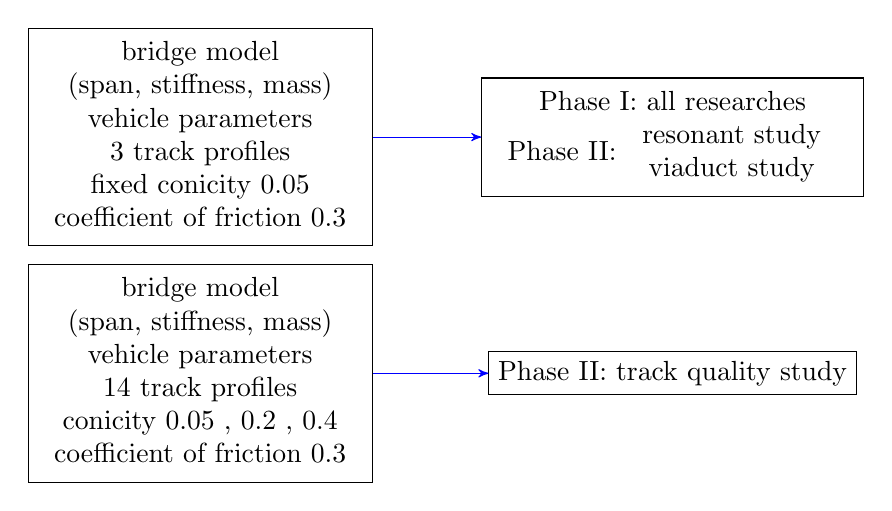
\begin{tikzpicture}

    \node[draw] (parameters) at (0,0) {
        \begin{tabular}{c}
            bridge model \\
            (span, stiffness, mass) \\
            vehicle parameters \\
            3 track profiles \\
            fixed conicity 0.05\\
            coefficient of friction 0.3 \\
        \end{tabular}
    };

    \node[draw] (phase I) at (6,0) {
        \begin{tabular}{c}
            Phase I: all researches \\
            Phase II: 
                \begin{tabular}{c}
                    resonant study\\
                    viaduct study\\
                \end{tabular} \\
        \end{tabular}
    };

    \node[draw] (phase II) at (6,-3) {Phase II: track quality study};

    \draw[->,draw=blue] (parameters) to (phase I);

    \node[draw] (parameters2) at (0,-3) {
        \begin{tabular}{c}
            bridge model \\
            (span, stiffness, mass) \\
            vehicle parameters \\
            14 track profiles \\
            conicity 0.05 , 0.2 , 0.4\\
            coefficient of friction 0.3 \\
        \end{tabular}
    };

    \draw[->,draw=blue] (parameters2) to (phase II);

\end{tikzpicture}

\caption{Overview of modelling setups for different studies conducted in DT329 }
\label{fig:modelling overview}
\end{figure}


\subsection{Model of bridge}
The bridge cases were modelled by assuming the bridges to behave as simply supported uniform beams. Transverse beam theory was then used to determine the frequencies and mode shapes of vibration for a given combination of span, mass per unit length and flexural rigidity. The modal information for the bridge was then used in a 'Normal Modes' analysis of the bridge.

For each case, all lateral modes of vibration up to and including 20 Hz were used. In order to prevent this artificially over-simplifying the model, if fewer than five modes were 20 Hz or less, all of the first five were used.

\subsection{Bridge parameters}

The spans considered were: 20 m, 33 m, 54 m, 90 m and 120 m. The flexibilities, defined as deflection of mid span over span length due to a static point load of 100 kN at mid span, are: 1/4000, 1/10000, and 1/20000. The mass per unit lengths required are: 2 tonnes/m, 6 tonnes/m, and 10 tonnes/m.

For the initial phase, see Figure \ref{fig:bridgeparametercombination} for a selection of eleven of the possible combinations examined.

\begin{figure}[h]
    \centering
    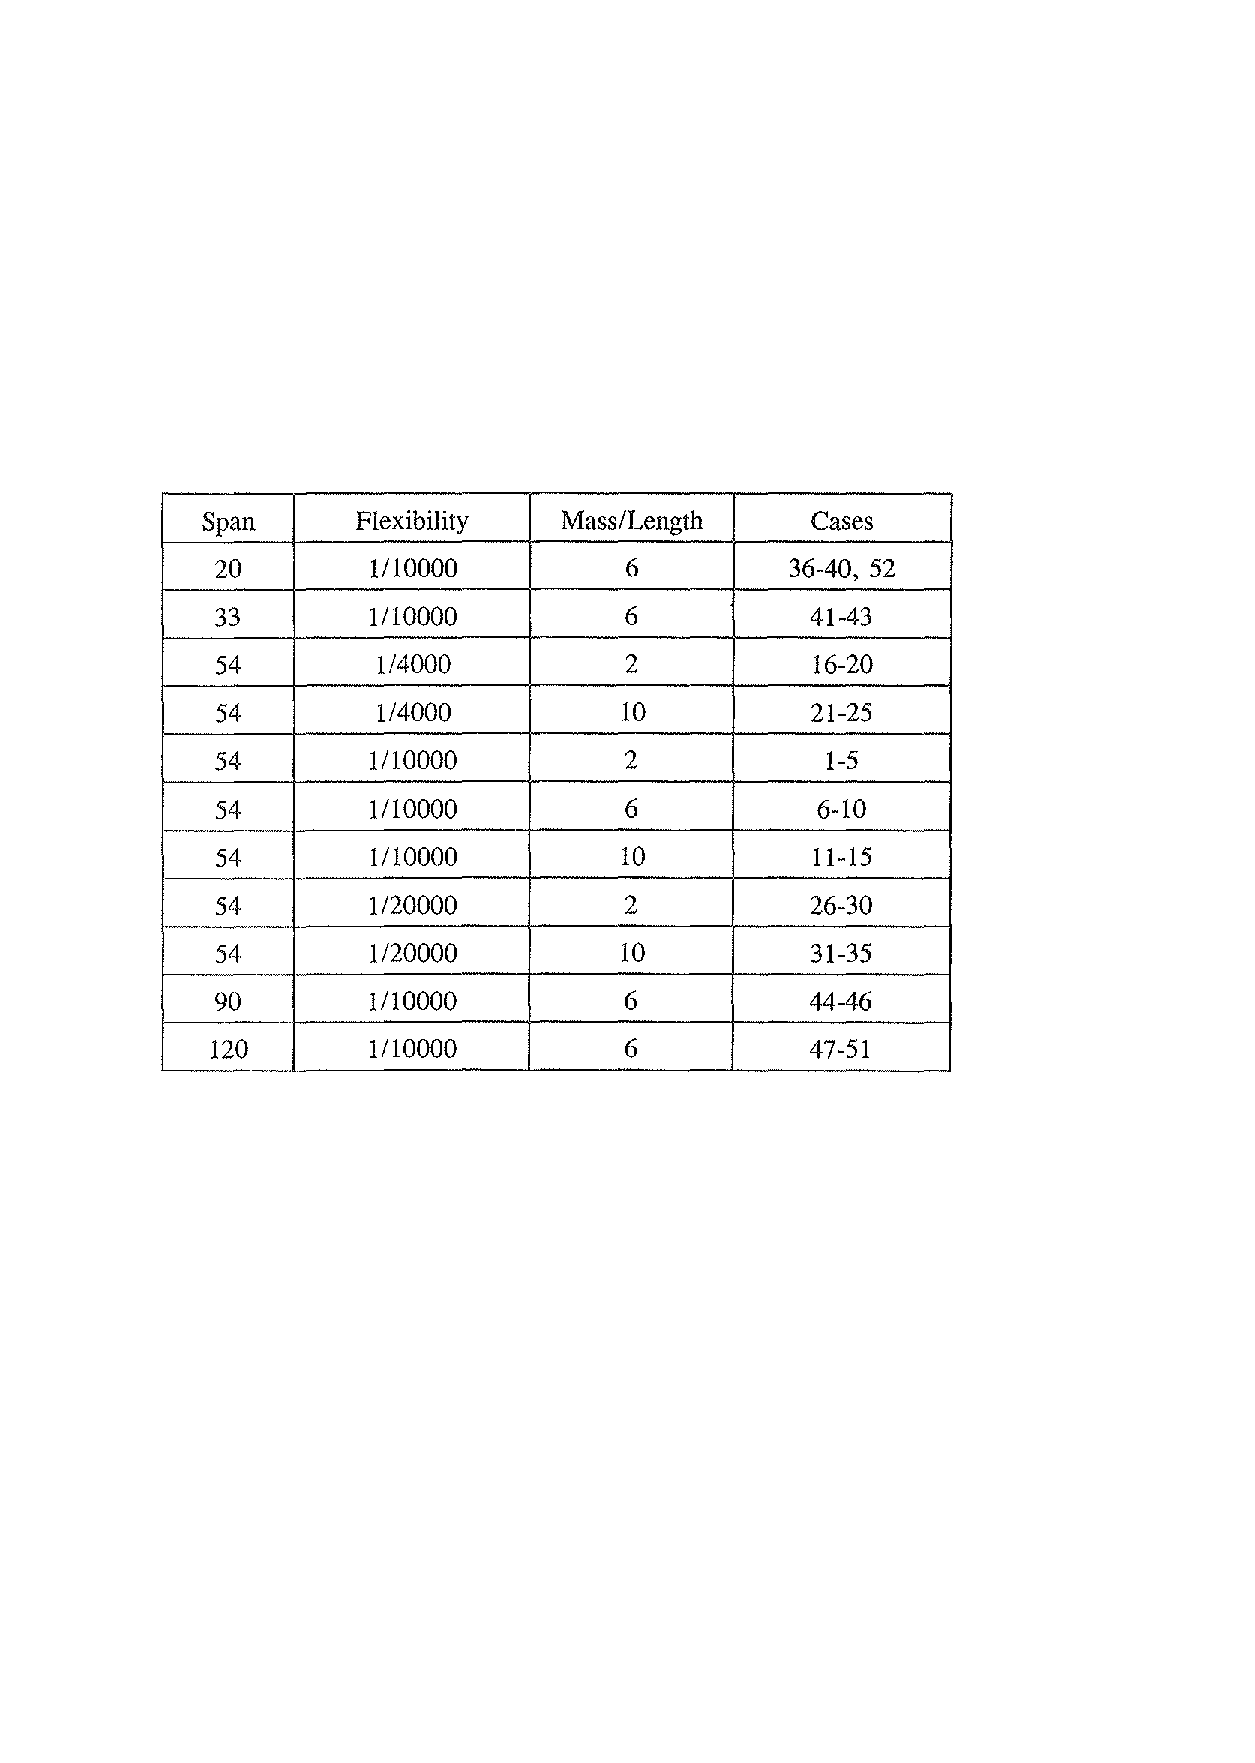
\includegraphics[width=\textwidth]{bridgeparametercombination}
    \caption{Bridge parameter combination}
    \label{fig:bridgeparametercombination}
\end{figure}

\subsection{Vehicle parameters}
Three train types are considered: a typical freight train, a typical standard passenger train, and a typical high speed passenger train. Appendix.\ref{app:dt329data} details the parameters used to construct each model. In general, each model consists of a locomotive and a number of identical vehicles appropriate to the train type. The total number of axles in each train is 24. Although effects on the train are only examined on the first vehicle of each type, extra vehicles are added to the train to see what cumulative effects occur to the bridge.

The freight train consists of a British Railways Class 56 locomotive and nine UIC wagons. This has a total length of 131.56 m, which assumes a nominal vehicle coupling distance of 4 m. Runs at 60 km/h and 100 km/h are required.

The standard passenger train consists of an E444 locomotive and five UIC coaches. This has a total length of 143.8 m. It is based on one of two train models used as part of the study of the FS Bridge discussed in report RP 3 of the Committee, differing only by the addition of three extra coaches. This is required to run at 160 km/h and 200 km/h.

The high speed passenger train consists of an ETR500 locomotive and five ETR500 coaches, having a total length of 145.8 m. It is based on the other FS bridge study train model mentioned above, differing from the original by an additional three ETR500 coaches. It is required to run at 300 km/h and 350 km/h.

\subsection{Track}

For initial study phase, the track samples used were consistent with each train type. PSD plots of each are shown in Figures \ref{fig:track1} to \ref{fig:track3}. Sample TRACKFRT.DAT was used for all analysis runs for the freight train. This is measured data from a typical BR freight line. Sample TRACKPN.DAT was used for the standard passenger train analysis runs. This is measured data from a part of the BR East Coast main line. Sample TRACKPH.DAT was used for high speed passenger train analysis runs. This is measured data from a typical DB high speed line.

Samples of 500 m were chosen so that there would be 100 m before the bridge and at least 100 m after the bridge for all combinations of span and train length. The initial 100 m is required to check vehicle behaviour on the track irregularity alone, and the portion after the train has left the bridge is required to check that the bridge vibrations decay.

For secondary study phase, the track data used to excite the mathematical models was taken from the British Rail Research library of measured track data. For the viaduct and resonance investigations, the track files used were the same as those used in the first part of the study. For the investigation of the influence of track quality, additional track data was used so as to give the widest possible range of realistic track qualities.

\subsection{Contact data}
For each run the same contact data was used, consisting of rails inclined at 1:20, and wheel profiles of conicity of 0.05 (based on standard British Rail 113A rails and PI wheel profiles). The coefficient of friction applied was 0.3.


\subsection{Data produced}

For every analysis run the following results were obtained at intervals of 0.01 seconds.

BRIDGE DATA:

Lateral displacement at mid span Lateral acceleration at mid span

\vspace*{\baselineskip}

VEHICLE LATERAL ACCELERATION DATA:

Loco body at leading pivot

Leading coach/wagon body at leading pivot/axle 

Loco leading bogie

Leading coach/wagon leading bogie/axle

\vspace*{\baselineskip}

TOTAL LATERAL FORCE DATA:

Loco leading bogie

Leading coach/wagon leading bogie/axle

\vspace*{\baselineskip}

LATERAL FORCES ON INDIVIDUAL WHEELS

Leading coach/wagon, first axle, left and right wheels 

Leading coach/wagon, second axle, left and right wheels 

Loco, first axle, left and right wheels

Loco, second axle, left and right wheels

\vspace*{\baselineskip}

In addition, for freight train runs, since the locomotive has two bogies of three axles, the forces on the individual wheels of the third axle were also produced.

Peak values for each of the outputs produced for the required ranges were obtained. For bridge outputs, peak values were taken for the period where any part of the train was on the bridge. For loco and leading coach/wagon outputs, peak values were taken whilst the vehicle in question was in contact with the bridge.

Peak values for each output were then read into a spread sheet where they could be compared more easily to check for emerging trends. The spread sheet has been partially automated to produce graphs of a single output for each train type for a single varying bridge parameter, for given values of the other bridge parameters. Figures 4 to 30 of original \citet{d181dt329} report show typical plots which have been produced in this manner.



\chapter{Plots and diagrams used in D181 DT 329}\label{app:dt329data}

\begin{figure}[h]
    \centering
    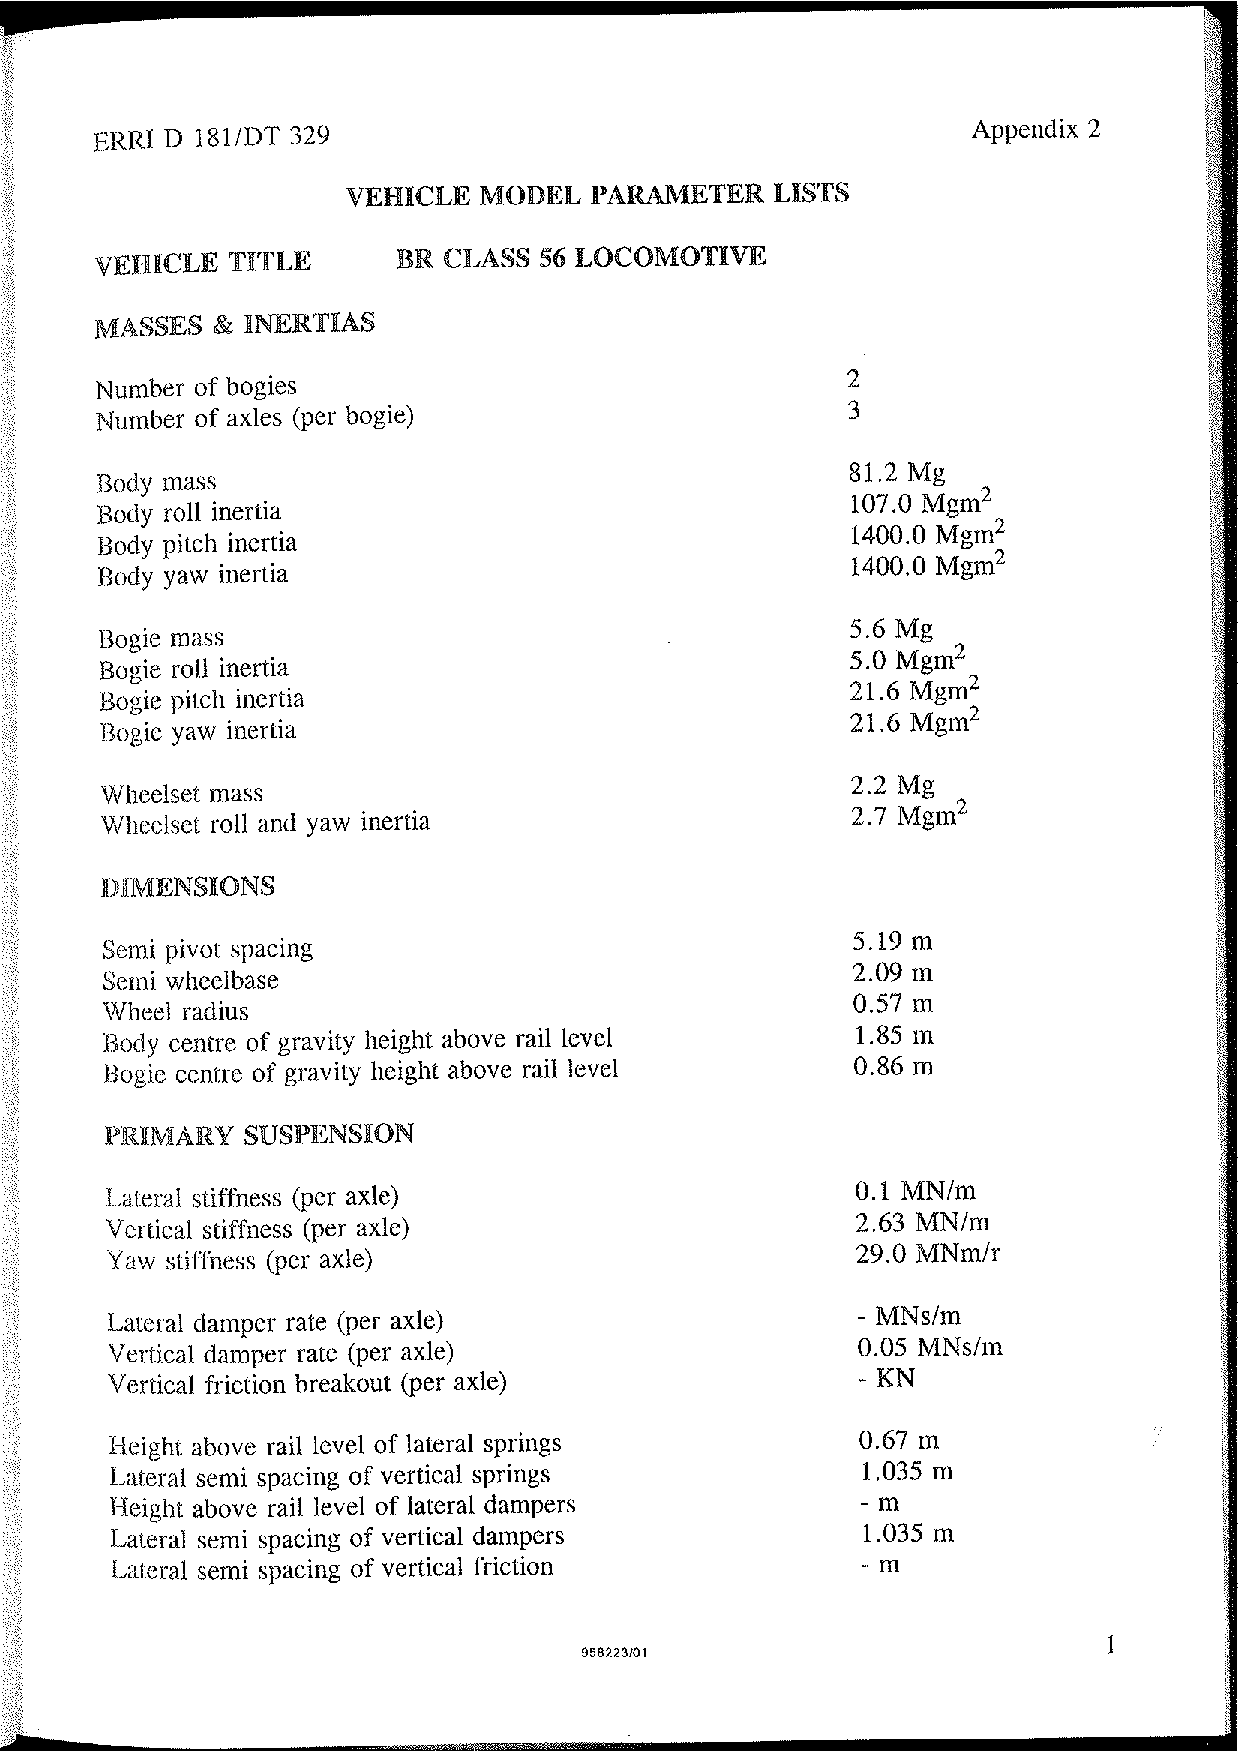
\includegraphics[width=\textwidth]{vp11}
    \caption{BR CLASS 56 LOCOMOTIVE. Extract from \citet[Appendix 2]{d181dt329}}
\end{figure}

\begin{figure}[h]
    \centering
    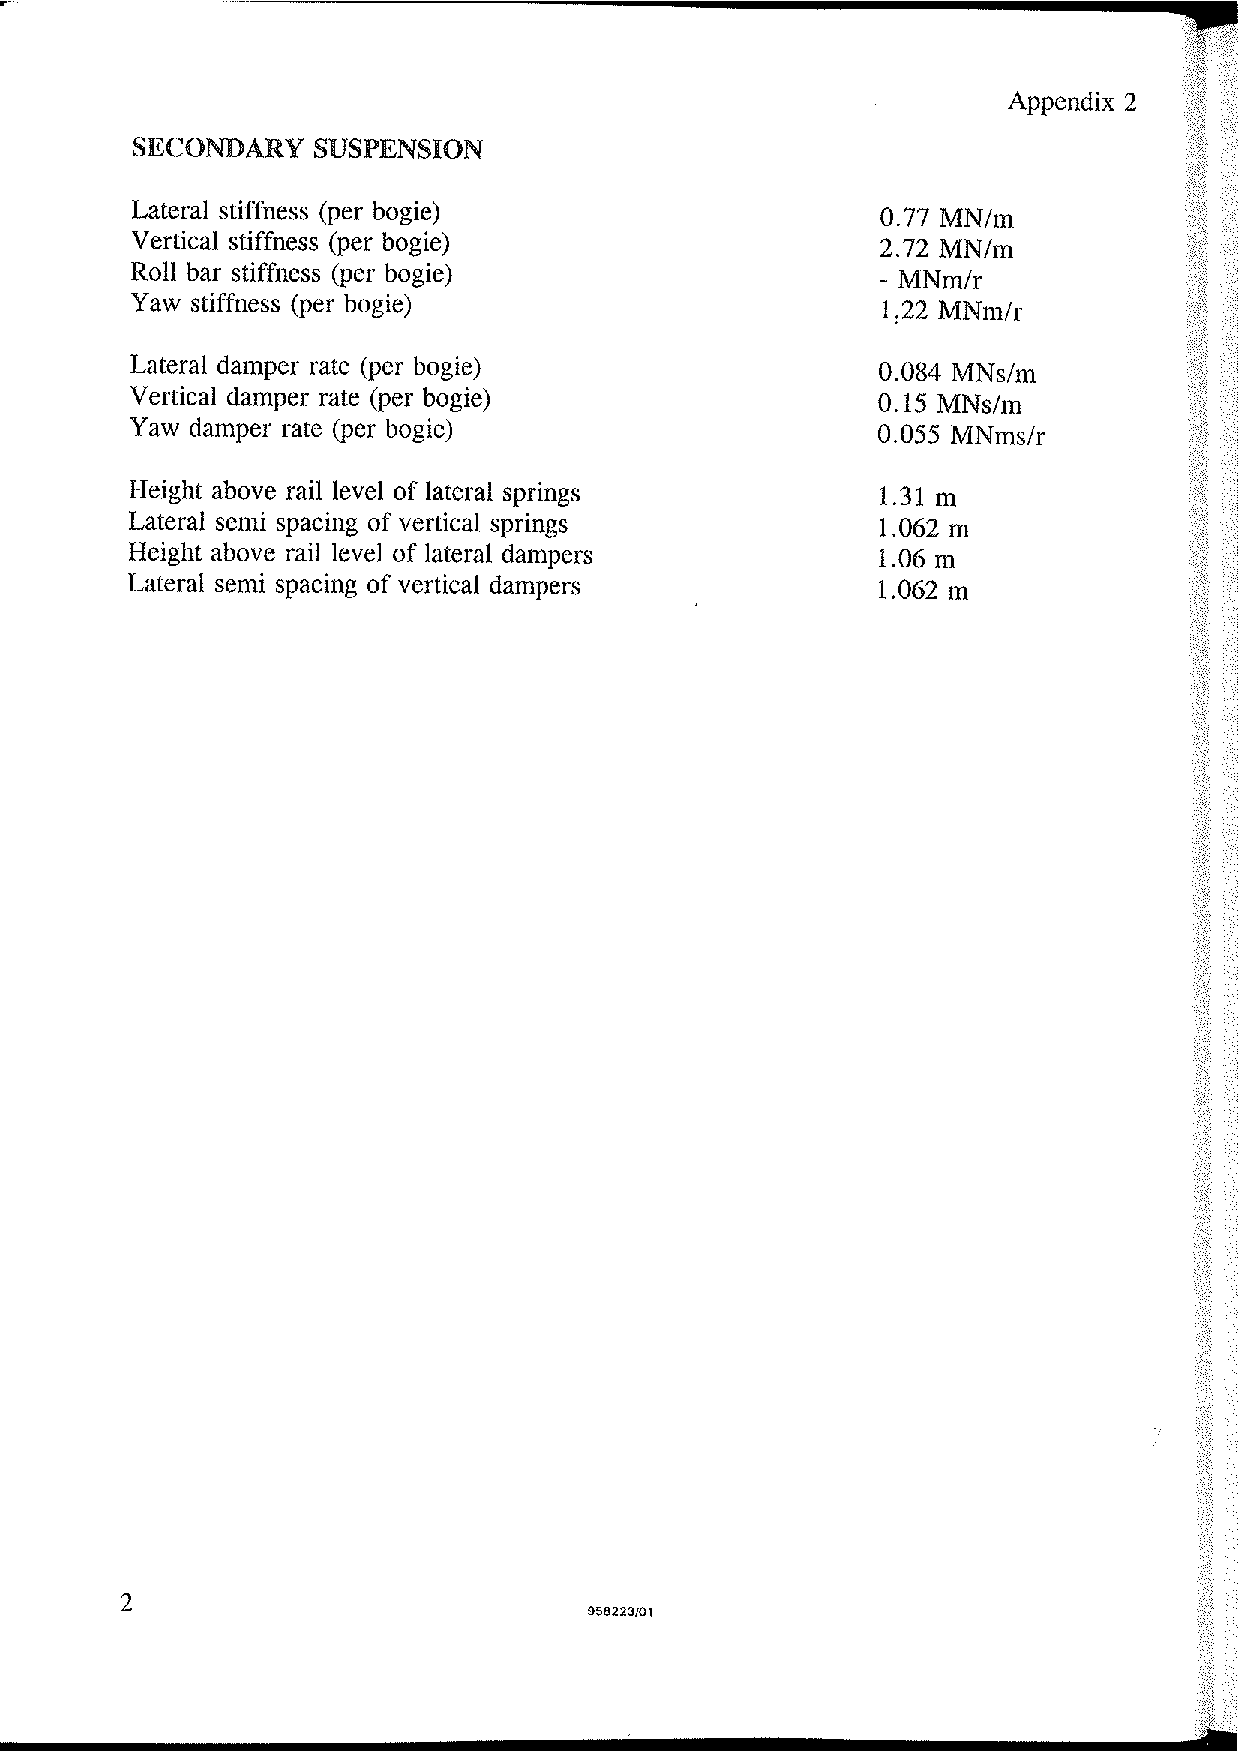
\includegraphics[width=\textwidth]{vp12}
    \caption{BR CLASS 56 LOCOMOTIVE. Extract from \citet[Appendix 2]{d181dt329}}
\end{figure}

\begin{figure}[h]
    \centering
    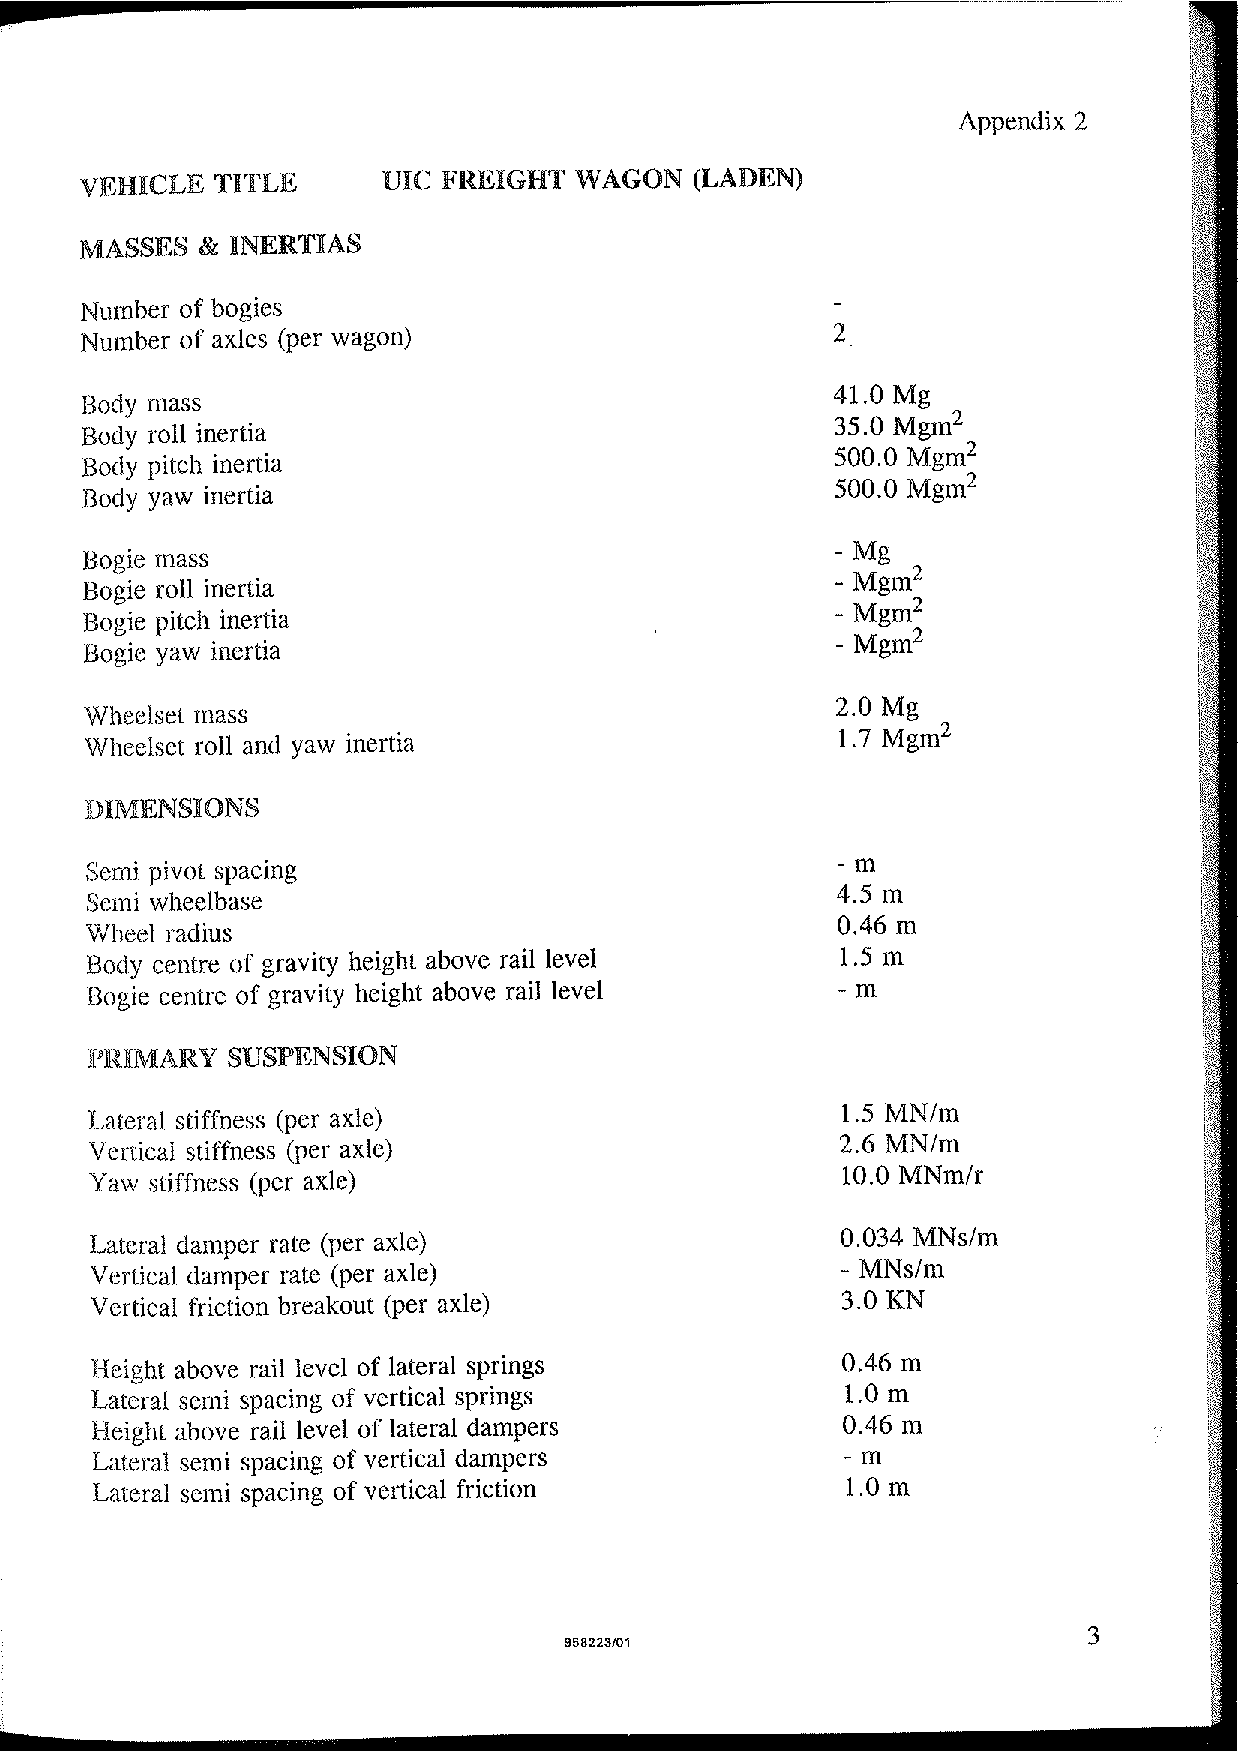
\includegraphics[width=\textwidth]{vp21}
    \caption{UIC FREIGHT WAGON (LADEN). Extract from \citet[Appendix 2]{d181dt329}}
\end{figure}

\begin{figure}[h]
    \centering
    \includegraphics[width=\textwidth]{vp22}
    \caption{UIC FREIGHT WAGON (LADEN). Extract from \citet[Appendix 2]{d181dt329}}
\end{figure}

\begin{figure}[h]
    \centering
    \includegraphics[width=\textwidth]{vp31}
    \caption{FS ETR500 LOCOMOTIVE. Extract from \citet[Appendix 2]{d181dt329}}
\end{figure}

\begin{figure}[h]
    \centering
    \includegraphics[width=\textwidth]{vp32}
    \caption{FS ETR500 LOCOMOTIVE. Extract from \citet[Appendix 2]{d181dt329}}
\end{figure}

\begin{figure}[h]
    \centering
    \includegraphics[width=\textwidth]{vp41}
    \caption{FS ETR500 COACH. Extract from \citet[Appendix 2]{d181dt329}}
\end{figure}

\begin{figure}[h]
    \centering
    \includegraphics[width=\textwidth]{vp42}
    \caption{FS ETR500 COACH. Extract from \citet[Appendix 2]{d181dt329}}
\end{figure}

\begin{figure}[h]
    \centering
    \includegraphics[width=\textwidth]{vp51}
    \caption{FS E444 LOCOMOTIVE. Extract from \citet[Appendix 2]{d181dt329}}
\end{figure}

\begin{figure}[h]
    \centering
    \includegraphics[width=\textwidth]{vp52}
    \caption{FS E444 LOCOMOTIVE. Extract from \citet[Appendix 2]{d181dt329}}
\end{figure}

\begin{figure}[h]
    \centering
    \includegraphics[width=\textwidth]{vp61}
    \caption{UIC COACH. Extract from \citet[Appendix 2]{d181dt329}}
    \label{fig:uicoach}
\end{figure}

\begin{figure}[h]
    \centering
    \includegraphics[width=\textwidth]{vp62}
    \caption{UIC COACH. Extract from \citet[Appendix 2]{d181dt329}}
\end{figure}

\begin{figure}[h]    \centering
    \includegraphics[width=\textwidth]{track1}
    \caption{Horizontal track irregularities for freight trains. Extract from \citet[Figure 2.1]{d181}}
    \label{fig:track1}
\end{figure}

\begin{figure}[h]
    \centering
    \includegraphics[width=\textwidth]{track2}
    \caption{Horizontal track irregularities for standard passenger trains. Extract from \citet[Figure 2.1]{d181}}
\end{figure}

\begin{figure}[h]
    \centering
    \includegraphics[width=\textwidth]{track3}
    \caption{Horizontal track irregularities for high speed passenger train. Extract from \citet[Figure 2.1]{d181}}
    \label{fig:track3}
\end{figure}

\begin{table}[h]
    \centering
    \begin{tabular}{c|c|c|c}
    \hline
    \multirow{2}{*}{Freight train: Principle axle repeat patterns} & dist & \multicolumn{2}{c}{Speed} \\
    & m & 60 km/h & 100 km/h \\
    \hline
    wagon n axle 2 - wagon n+1 axle 1 & 4.00 & 4.17 & 6.94 \\
    wagon wheelbase & 9.00 & 1.85 & 3.09 \\
    wagon n axle m - wagon n+1 axle m & 13.0 & 1.28 & 2.14 \\
    wagon n axle m - wagon n+2 axle m & 26.0 & 0.64 & 1.07 \\
    \hline
    \multirow{2}{*}{Passenger train: Principle axle repeat patterns} & dist & \multicolumn{2}{c}{Speed} \\
    & m & 160 km/h & 200 km/h \\
    \hline
    coach n axle 1 - 2, and coach n axle 3 - 4 & 2.56 & 17.36 & 21.70 \\
    coach n axle m - coach n+1 axle m & 26.4 & 1.68 & 2.10 \\
    coach n axle m - coach n+2 axle m & 52.8 & 0.84 & 1.05 \\
    \hline
    \multirow{2}{*}{ETR 500 train: Principle axle repeat patterns} & dist & \multicolumn{2}{c}{Speed} \\
    & m & 300 km/h & 350 km/h \\
    \hline
    coach n axle 1 - 2 and coach n axle 3 - 4 & 3.0 & 27.78 & 32.41 \\
    coach n axle m - coach n+1 axle m & 26.1 & 3.19 & 3.72 \\
    coach n axle m - coach n+2 axle m & 52.2 & 1.60 & 1.86 \\
    coach n axle m - coach n+3 axle m & 69.3 & 1.20 & 1.40 \\
    \hline
    \end{tabular}
    \caption{Axle repeat patterns and typical frequencies. Extracted from \citet[Appendix C]{d181dt329}}
    \label{tab:329axlerepeat}
\end{table}

\begin{table}[h]
    \centering
    \begin{tabular}{c|c|c|c}
    \hline
    Kinematic wavelength, m & Freight train & Passenger train & ETR500 train \\
    \hline
    Locomotive & 39 - 45 & 32 - 38 & 39 - 45 \\
    Coach/wagon & 24 - 39 & 34 - 38 & 36 - 40 \\
    \hline
    \end{tabular}
    \caption{Kinematic wavelength ranges per vehicle, with BR P1 profiles. Extracted from \citet[Appendix C]{d181dt329}}
    \label{tab:329kinematicwavelength}
\end{table}

% \chapter{Essentials of analytical approach to be adopted in practical checking method}\label{sec:analyticalmodel}
 
% \section{Introduction}
% This chapter aims to give a preliminary knowledge of a selected analytical model that simulates the perfect resonance scenario for railway bridge under lateral dynamic load. The knowledge contains the simplified model itself, its assumptions, field of application and explicit solutions. 

% The output response of the solution to the analytical model is able to provide the maximum bridge response in worst case scenario. Thus it is sufficient to be adopted in practical purposes for verifications of lateral railway bridge dynamics.


% \section{Overview}

% To give a clear view of this chapter, following overview is created:

% \begin{enumerate}
%     \item The model, its assumptions and field of application. 
%     \item Procedure of solution deduction
%     \item Damping
% \end{enumerate}

% \section{The model, its assumptions and field of application}

% \begin{figure}[h]
%     \centering
%     \includegraphics[width=0.5\textwidth]{harmonicloadbeam}
%     \caption{Schematic representation of a generic beam crossed by a harmonic load}
%     % \label{fig:harmonicloadbeam}
% \end{figure}

% Presented in Figure.\ref{fig:harmonicloadbeam}, the model features a simply supported beam which is the simplification of bridge structure and a moving harmonic load introducing resonant dynamic effects caused by the presence of moving train.

% The beam is assumed to be uniform in both geometry and material. The stiffness of the beam is the equivalent uniform lateral bending stiffness of the bridge. 

% The load is moving in the same speed as the train. The magnitude of load amplitude is going to be discussed in the following chapter. The load's self vibration frequency is equal to the first natural lateral bending frequency of the beam.


% This model is valid for single span railway bridges that has a sinuous first natural lateral vibration shape.  

% \section{Solution deduction}

% Solution provided by Fryba\citet{fryba1999vibration} is used to analyse the problem. A harmonic moving along a beam is a fundamental dynamics topic and was first solved by S.P.Timoshenko. Fryba further deduced the basic results, and set them forth in the form of useful formulae. This model is used to simulate a perfect resonance scenario which yields conservative results for designing and checking of the dynamics behaviour of the bridge. Deduction procedure is extracted from \citet[Section II.2.1]{fryba1999vibration} and presented below.

% \begin{quote}

% The solution of the problem of a harmonic concentrated force moving at constant speed $c$ over a simply supported beam with span $l$ is carried out under the same assumptions as that discussed in Chap. 1. The time-variable concentrated force is of the form

% \begin{equation}%\label{eq:equationofmotion}
%     P(t) = Q \sin \Omega t
% \end{equation}

% where $Q$ is the amplitude and $\Omega$ is the circular frequency of the harmonic force. Vibration of the beam is then described by the equation

% \begin{equation}
%     EJ\frac{\partial^4 v(x,t)}{\partial x^4} + \mu\frac{\partial^2 v(x,t)}{\partial t^2} +2\mu\omega_b \frac{\partial v(x,t)}{\partial t} = \delta(x-ct)Q\sin\Omega t 
% \end{equation}

% by the boundary conditions (1.2) and by the initial conditions (1.3). The symbols used in \ref{eq:equationofmotion} have the same meaning as those of Chap. 1.

% Eq.\ref{eq:equationofmotion} together with conditions (1.2) and (1.3) will again be solved by the method of integral transformations. Following the Fourier sine transformation according to (1.9), Eqs.\ref{eq:equationofmotion} and (1.2) give

% \begin{equation}
%     \frac{d^2 V(j,t)}{d t^2} + 2\omega_b\frac{dV(j,t)}{dt} + \omega_{(j)}^2 V(j,t) = \frac{Q}{\mu} \sin\Omega t \sin j\omega t
% \end{equation}

% Solving the above with (1.3) by the Laplace-Carson transformation (1.15) - making use of Eq.(27.24) in doing so and of the notation

% \begin{equation}
%     \begin{tabular}{cc}
%         $r_1 = \Omega + j\omega$; & $r_2 = \Omega - j\omega$ \\
%     \end{tabular}
% \end{equation}

% we get

% \begin{equation}\label{eq:V*}
%     V^* (j,p) = \frac{Q}{2\mu} (\frac{1}{p^2+r_2^2}-\frac{1}{p^2+r_1^2})\frac{p^2}{(p+\omega_b)^2+\omega_{(j)}^{'2}}
% \end{equation}

% After inverse transformations of Eq.\ref{eq:V*} according to (27.24) and (1.9) the required result for $t \leq T$ is

% \begin{dmath}\label{eq:v(x,t)complicated}
%     v(x,t) = \sum_{j=1}^{\infty} \frac{Q}{\mu l}\{\frac{1}{(\omega_{(j)}^2 - r_2^2)+4\omega_b^2r_2^2}[(\omega_{j}^2-r_2^2])(\cos r_2t-e^{-\omega_bt}\cos \omega_{(j)}^' t) + 2\omega_b r_2 \sin r_2 t - \frac{\omega_b}{\omega_{(j)}^'}(\omega_{(j)}^2 + r_2^2)e^{-\omega_b t}\sin \omega_{(j)}^'t]-\frac{1}{(\omega_{(J)}^2 - r_1^2)^2 + 4\omega_b^2r_1^2}[(\omega_{(j)}^2-r_1^2)(\cos r_1t-e^{-\omega_b t}\cos\omega{(j)}^'t)+2\omega_b r_1 \sin r_1 t- \frac{\omega_b}{\omega_{(j)}^'}(\omega_{(j)}^2+r_1^2)e^{-\omega_b t}\sin \omega_{(j)}^' t]\}\sin\frac{j\pi x}{l}
% \end{dmath}

% We shall now simplify Eq.\ref{eq:v(x,t)complicated} to fit the case most frequently met with in practical applications. Thus, for example, it is entirely satisfactory to use only the first of its terms($j=1$); further, as we know from Chap. 1, parameters $\alpha$ and $\beta$ are usually much smaller than 1 ($\alpha = \sfrac{\omega}{\omega_{(1)}} \ll 1$, $\beta = \sfrac{\omega_b}{\omega_{(1)}} \ll 1$). And finally, since in practice a harmonic force is always accompanied by a constant force $P$, we shall introduce in \ref{eq:v(x,t)complicated} also the deflection $v_0$ according to (1.21). Following these simplifications Eq.(2.6) takes on the form

% \begin{dmath}\label{eq:v(x,t)withP}
% v(x,t) = v_0 \frac{Q}{p}\frac{\omega_{(1)}^2}{\Omega^2}\frac{1}{(\frac{\omega_{(1)}^2}{\Omega^2}-1)^2+4(\frac{\omega^2}{\Omega^2}+\frac{\omega_b^2}{\Omega^2})}\{[(\frac{\omega_{(1)}^2}{\Omega^2}-1)^2+4\frac{\omega_b^2}{\Omega^2}]^{\sfrac{1}{2}} \sin (\Omega t + \varphi)\sin \omega t + 2\frac{\omega}{\Omega}(\cos \Omega t \cos \omega t - e^{-\omega_b t}\cos \omega_{(1)}t)\}\sin\frac{\pi x}{l}
% \end{dmath}

% where

% \begin{equation}
%     \tan \varphi = -\frac{2\sfrac{\omega_b}{\Omega}}{\sfrac{\omega_{(1)}^2}{\Omega^2}-1}
% \end{equation}

% The beam reaches the state of highest dynamic stressing in the region of resonance, i.e. whenever $\Omega$ is close or just equal to $\omega_{(1)}$, i.e.

% \begin{equation}
%     \Omega = \omega_{(1)}
% \end{equation}

% In such a case Eq.\ref{eq:v(x,t)withP} can further be simplified to 

% \begin{equation}\label{eq:v(x,t)simplewithP}
%     v(x,t) = v_0 \frac{Q\omega_{(1)}}{2P}\frac{\cos \omega_{(1)}t}{\omega^2+\omega_b^2}[\omega(\cos\omega t - e^{-\omega_b t})-\omega_b\sin\omega t]\sin\frac{\pi x}{l}
% \end{equation}

% \end{quote}

% According to (1.21)

% \begin{equation}
%     v_0 = \frac{Pl^3}{48EJ} \approx \frac{2P}{\mu l \omega_{(1)}^2} = \frac{2Pl^3}{\pi ^4 EJ}
% \end{equation}

% substitute $v_0$ into Eq.\ref{eq:v(x,t)simplewithP}

% \begin{equation}
%     v(x,t) = \frac{l^3Q\omega_{(1)}}{\pi^4 EJ}\frac{\cos \omega_{(1)}t}{\omega^2+\omega_b^2}[\omega(\cos\omega t - e^{-\omega_b t})-\omega_b\sin\omega t]\sin\frac{\pi x}{l}
% \end{equation}

% And the mid-span response time-history for deflection is :

% \begin{equation}%\label{eq:v(x,t)simpleharmonic}
%     v(\sfrac{l}{2},t) = \frac{l^3Q\omega_{(1)}}{\pi^4 EJ}\frac{\cos \omega_{(1)}t}{\omega^2+\omega_b^2}[\omega(\cos\omega t - e^{-\omega_b t})-\omega_b\sin\omega t]
% \end{equation}

% where:

% $v$ : deflection of the beam($m$)

% $l$ : span of the beam($m$)

% $EJ$ : lateral stiffness of the beam($Nm^2$)

% $Q$ : amplitude of harmonic load($N$)

% $c$ : speed of the train($m/s$)

% $\zeta$ : damping ratio

% $\mu$ : mass per unit length of the beam($kg/m$)

% $\omega_1$ : first natural circular frequency of the beam

% $\omega_1=\frac{\pi^2}{l^2}\sqrt{\frac{EJ}{\mu}}$

% $\omega = \sfrac{\pi c}{l}$

% $\omega_b = \frac{1}{2}\zeta\omega_1 $


 
% Above expression is the ready-to-use expression being adopted in practical checking method to be discussed in following chapter.


% \section{Damping}
% Damping is an important parameter influencing the dynamic behaviour of a structure. \ref{eq:equationofmotion} uses a different form of damping expression $\omega_b$, which can be converted from normal damping coefficient. Equation of motion using damping coefficient:

% \begin{equation}%\label{eq:equationofmotiondampingcoefficient}
%     EJ\frac{\partial^4 v(x,t)}{\partial x^4} + \mu\frac{\partial^2 v(x,t)}{\partial t^2} +\chi \frac{\partial v(x,t)}{\partial t} = \delta(x-ct)Q\sin\Omega t 
% \end{equation}

% where $\chi$ stands for damping coefficient. By comparing \ref{eq:equationofmotiondampingcoefficient} and \ref{eq:equationofmotion}:

% \begin{equation}
%     \omega_b = \frac{\chi}{2\mu}
% \end{equation}

% where:

% $\omega_b$: circular frequency of damping

% $\chi$: damping coefficient

% $\mu$: mass per unit length of the bridge

% also, in \citet[Page.704]{abu2000vibration} it is mentioned that:

% \begin{quote}
%     The external and internal damping of the beam are assumed to be proportional to the mass and stiffness of the beam respectively,i.e., $r_a = \gamma_1 \mu$.., where $\gamma_1$ and $\gamma_2$ are proportionality constants.
% \end{quote}

% thus:


% \begin{equation}
%     \omega_b = \frac{\gamma_1}{2}
% \end{equation}

% and it is mentioned in \citet[Eq.8]{abu2000vibration} that:

% $$\zeta = \frac{\gamma_1}{\omega_1}$$

% so:

% $$\gamma_1 = \zeta\omega_1$$

% so:

% $$\omega_b = \frac{1}{2}\zeta\omega_1 = \frac{1}{2}\frac{\zeta\pi^2}{l^2}\sqrt{\frac{EJ}{\mu}}$$

% where $\zeta$ is the structure damping ratio stated in EN1991-

% Adopting $\zeta = 1\%$ for steel railway bridges. This $\zeta$ value is used among all DT329 simulations run files. See Figure.\ref{fig:examplerunfile} for example.
% T329 resonance study. By comparing with the output of reproduced resonance in DT329, the analytical model can be verified.

% \section{Verification of the explicit solution}
% Since circular frequency of damping $\omega_b$ is not clearly defined by Fryba, it is necessary to verify the correctness of both explicit solution and deduced $\omega_b$ expression.

% The verification is done by comparing the result of Eq.\ref{eq:v(x,t)simpleharmonic} with the result of a explicit solution in a different form obtained by another deducing method.  

% The result in \citet{abu2000vibration} is selected to compare. This report is researching vibration of beams with general boundary conditions due to a moving harmonic load. The differential equation is illustrated as follows:

% \begin{equation}\label{eq:hilal}
%     EIv''''+\mu \ddot{v} + r_a \dot{v}+r_i \dot{v}''' = p(x,t)
% \end{equation}

% The difference between Eq.\ref{eq:hilal} and Eq.\ref{eq:v(x,t)simpleharmonic} is that it offers broader boundary conditions such as changing speed of the load and various kinds of supports. As a result of more general equation, the deduction steps are much more complicated. However, two solutions should yield same results under same boundary conditions that:

% \begin{enumerate}
%     \item Load moving at constant speed,
%     \item Frequency of load equals frequency of the beam,
%     \item Internal damping is 0,
%     \item Simple hinge support at both ends of the beam.
% \end{enumerate}

% One plot from the parametric study of \citet{abu2000vibration} meets the above requirement and is selected and illustrated in Figure. Parameter used in this plot is $\alpha = 0.25$, $\zeta = 0.05$, $\beta  = 1$

% \begin{figure}[h!]
%     \centering
%     \includegraphics[width=0.5\textwidth]{hilalplot}
%     \caption{Reference plot extracted from \citet{abu2000vibration}. Condition: $\alpha = 0.25$, $\zeta = 0.05$, $\beta  = 1$. Y axis for dynamic amplification factor.}
%     \label{fig:hilalplot}
% \end{figure}

% Next step is to translate parameters used in above plot to usable parameters in Eq.\ref{eq:v(x,t)simpleharmonic}.


% $$c_{cr} = \frac{\omega_1 L}{\pi} = \frac{\pi}{l}\sqrt{\frac{EJ}{\mu}}$$

% $$\alpha = \frac{c}{c_{cr}}$$

% $$c = \alpha c_{cr} = \frac{\alpha\pi}{l}\sqrt{\frac{EJ}{\mu}}$$

% $EJ$,$\mu$,$l$ needs to be selected to yield value for $c$, thus following values are randomly selected:

% $$EJ = 2.43e10 Nm^2$$

% $$l = 54m$$

% $$\mu = 6000 kg/m$$

% $$c_{cr} = 117.05 m/s$$

% $$ c = 29.26 m/s $$

% A Matlab script is written to automate numerical calculating procedure. By typing 

% \texttt{fogtest(2.43e10,54,6000,29.26,0.05)}

% into the console. Figure.\ref{fig:EJ24300000000L54mu6000c29daf.tikz} is obtained.

% \begin{figure}[h!]
% \centering 
% \setlength\figureheight{6cm} 
% \setlength\figurewidth{6cm} 
% % This file was created by matlab2tikz v0.4.7 (commit 949a076472a7bec3ddc3d4cd9cc5273c97709f91) running on MATLAB 8.3.
% Copyright (c) 2008--2014, Nico Schlmer <nico.schloemer@gmail.com>
% All rights reserved.
% Minimal pgfplots version: 1.3
% 
\begin{tikzpicture}

\begin{axis}[%
width=\figurewidth,
height=\figureheight,
scale only axis,
xmin=0,
xmax=2,
ymin=-4,
ymax=4
]
\addplot [color=blue,solid,forget plot]
  table[row sep=crcr]{%
0	0\\
0.00186206896551724	-9.81557918731428e-06\\
0.00372413793103448	-3.92485973868528e-05\\
0.00558620689655172	-8.82641320004888e-05\\
0.00744827586206897	-0.000156808154525201\\
0.00931034482758621	-0.000244807560818895\\
0.0111724137931034	-0.000352170209420864\\
0.0130344827586207	-0.000478784967915698\\
0.0148965517241379	-0.000624521767319481\\
0.0167586206896552	-0.000789231664470319\\
0.0186206896551724	-0.000972746912398953\\
0.0204827586206897	-0.00117488103865367\\
0.0223448275862069	-0.00139542893155333\\
0.0242068965517241	-0.0016341669343347\\
0.0260689655172414	-0.0018908529471638\\
0.0279310344827586	-0.00216522653697387\\
0.0297931034482759	-0.00245700905508991\\
0.0316551724137931	-0.00276590376260297\\
0.0335172413793103	-0.00309159596344666\\
0.0353793103448276	-0.00343375314513037\\
0.0372413793103448	-0.00379202512708536\\
0.0391034482758621	-0.00416604421656322\\
0.0409655172413793	-0.00455542537204366\\
0.0428275862068965	-0.0049597663740878\\
0.0446896551724138	-0.00537864800358338\\
0.046551724137931	-0.00581163422731614\\
0.0484137931034483	-0.0062582723908105\\
0.0502758620689655	-0.00671809341836777\\
0.0521379310344828	-0.00719061202023671\\
0.054	-0.00767532690684718\\
0.0558620689655172	-0.00817172101002975\\
0.0577241379310345	-0.0086792617111522\\
0.0595862068965517	-0.00919740107609054\\
0.061448275862069	-0.00972557609695757\\
0.0633103448275862	-0.0102632089405056\\
0.0651724137931034	-0.0108097072031222\\
0.0670344827586207	-0.0113644641723273\\
0.0688965517241379	-0.0119268590946905\\
0.0707586206896552	-0.0124962574500712\\
0.0726206896551724	-0.0130720112320935\\
0.0744827586206896	-0.0136534592347589\\
0.0763448275862069	-0.0142399273451013\\
0.0782068965517241	-0.0148307288417832\\
0.0800689655172414	-0.0154251646995372\\
0.0819310344827586	-0.0160225238993431\\
0.0837931034482759	-0.0166220837442425\\
0.0856551724137931	-0.0172231101806802\\
0.0875172413793103	-0.0178248581252654\\
0.0893793103448276	-0.0184265717968423\\
0.0912413793103448	-0.019027485053758\\
0.0931034482758621	-0.0196268217362131\\
0.0949655172413793	-0.0202237960135815\\
0.0968275862068965	-0.0208176127365785\\
0.0986896551724138	-0.0214074677941622\\
0.100551724137931	-0.0219925484750448\\
0.102413793103448	-0.0225720338336929\\
0.104275862068966	-0.0231450950606914\\
0.106137931034483	-0.0237108958573492\\
0.108	-0.024268592814415\\
0.109862068965517	-0.0248173357947798\\
0.111724137931034	-0.0253562683200327\\
0.113586206896552	-0.0258845279607415\\
0.115448275862069	-0.026401246730324\\
0.117310344827586	-0.0269055514823772\\
0.119172413793103	-0.0273965643113307\\
0.121034482758621	-0.0278734029562845\\
0.122896551724138	-0.0283351812078991\\
0.124758620689655	-0.0287810093181939\\
0.126620689655172	-0.0292099944131192\\
0.12848275862069	-0.0296212409077586\\
0.130344827586207	-0.03001385092402\\
0.132206896551724	-0.0303869247106758\\
0.134068965517241	-0.0307395610656031\\
0.135931034482759	-0.0310708577600861\\
0.137793103448276	-0.0313799119650312\\
0.139655172413793	-0.0316658206789497\\
0.14151724137931	-0.0319276811575626\\
0.143379310344828	-0.0321645913448785\\
0.145241379310345	-0.0323756503055976\\
0.147103448275862	-0.0325599586586926\\
0.148965517241379	-0.0327166190120181\\
0.150827586206897	-0.0328447363977961\\
0.152689655172414	-0.0329434187088317\\
0.154551724137931	-0.0330117771353033\\
0.156413793103448	-0.0330489266019807\\
0.158275862068966	-0.0330539862057153\\
0.160137931034483	-0.0330260796530559\\
0.162	-0.0329643356978319\\
0.163862068965517	-0.0328678885785568\\
0.165724137931034	-0.0327358784554969\\
0.167586206896552	-0.0325674518472536\\
0.169448275862069	-0.0323617620667063\\
0.171310344827586	-0.0321179696561639\\
0.173172413793103	-0.0318352428215708\\
0.175034482758621	-0.0315127578656171\\
0.176896551724138	-0.0311496996195988\\
0.178758620689655	-0.0307452618738761\\
0.180620689655172	-0.030298647806778\\
0.18248275862069	-0.029809070411802\\
0.184344827586207	-0.0292757529229552\\
0.186206896551724	-0.0286979292380885\\
0.188068965517241	-0.0280748443400706\\
0.189931034482759	-0.0274057547156529\\
0.191793103448276	-0.026689928771875\\
0.193655172413793	-0.0259266472498608\\
0.19551724137931	-0.0251152036358579\\
0.197379310344828	-0.0242549045693701\\
0.199241379310345	-0.0233450702482374\\
0.201103448275862	-0.0223850348305153\\
0.202965517241379	-0.0213741468330077\\
0.204827586206897	-0.0203117695263084\\
0.206689655172414	-0.0191972813262065\\
0.208551724137931	-0.0180300761813122\\
0.210413793103448	-0.0168095639567602\\
0.212275862068966	-0.015535170813849\\
0.214137931034483	-0.0142063395854758\\
0.216	-0.012822530147227\\
0.217862068965517	-0.0113832197839859\\
0.219724137931034	-0.0098879035519203\\
0.221586206896552	-0.0083360946357138\\
0.223448275862069	-0.00672732470090573\\
0.225310344827586	-0.00506114424120609\\
0.227172413793103	-0.00333712292065325\\
0.229034482758621	-0.00155484991048313\\
0.230896551724138	0.000286065779419632\\
0.232758620689655	0.00218599497461664\\
0.234620689655172	0.00414528801588362\\
0.23648275862069	0.00616427444477682\\
0.238344827586207	0.00824326269512078\\
0.240206896551724	0.0103825397905403\\
0.242068965517241	0.0125823710481567\\
0.243931034482759	0.0148429997885672\\
0.245793103448276	0.0171646470522243\\
0.247655172413793	0.0195475113223312\\
0.24951724137931	0.0219917682543657\\
0.251379310344828	0.0244975704123454\\
0.253241379310345	0.027065047011943\\
0.255103448275862	0.0296943036705609\\
0.256965517241379	0.0323854221644705\\
0.258827586206897	0.0351384601931194\\
0.260689655172414	0.0379534511507114\\
0.262551724137931	0.0408304039051558\\
0.264413793103448	0.0437693025844865\\
0.266275862068966	0.0467701063708472\\
0.268137931034483	0.0498327493021337\\
0.27	0.0529571400813884\\
0.271862068965517	0.0561431618940342\\
0.273724137931035	0.059390672233036\\
0.275586206896552	0.0626995027320748\\
0.277448275862069	0.0660694590068173\\
0.279310344827586	0.0695003205043603\\
0.281172413793103	0.0729918403609313\\
0.283034482758621	0.076543745267916\\
0.284896551724138	0.0801557353462911\\
0.286758620689655	0.0838274840295311\\
0.288620689655172	0.0875586379550571\\
0.29048275862069	0.0913488168642963\\
0.292344827586207	0.0951976135114118\\
0.294206896551724	0.0991045935807694\\
0.296068965517241	0.103069295613194\\
0.297931034482759	0.107091230941078\\
0.299793103448276	0.111169883632387\\
0.301655172413793	0.115304710443627\\
0.30351724137931	0.119495140781804\\
0.305379310344828	0.123740576675438\\
0.307241379310345	0.128040392754662\\
0.309103448275862	0.13239393624046\\
0.310965517241379	0.136800526943065\\
0.312827586206897	0.141259457269567\\
0.314689655172414	0.145769992240753\\
0.316551724137931	0.150331369517218\\
0.318413793103448	0.154942799434769\\
0.320275862068966	0.159603465049135\\
0.322137931034483	0.164312522190035\\
0.324	0.169069099524586\\
0.325862068965517	0.173872298630094\\
0.327724137931034	0.17872119407623\\
0.329586206896552	0.1836148335166\\
0.331448275862069	0.188552237789721\\
0.333310344827586	0.193532401029408\\
0.335172413793103	0.198554290784571\\
0.337034482758621	0.203616848148417\\
0.338896551724138	0.208718987897069\\
0.340758620689655	0.213859598637574\\
0.342620689655172	0.219037542965308\\
0.34448275862069	0.224251657630757\\
0.346344827586207	0.229500753715663\\
0.348206896551724	0.23478361681851\\
0.350068965517241	0.240099007249341\\
0.351931034482759	0.245445660233871\\
0.353793103448276	0.250822286126875\\
0.355655172413793	0.256227570634824\\
0.35751724137931	0.261660175047732\\
0.359379310344828	0.267118736480177\\
0.361241379310345	0.272601868121471\\
0.363103448275862	0.278108159494919\\
0.364965517241379	0.283636176726144\\
0.366827586206897	0.289184462820415\\
0.368689655172414	0.294751537948938\\
0.370551724137931	0.300335899744058\\
0.372413793103448	0.305936023603311\\
0.374275862068966	0.311550363002279\\
0.376137931034483	0.317177349816177\\
0.378	0.322815394650113\\
0.379862068965517	0.328462887177965\\
0.381724137931034	0.334118196489785\\
0.383586206896552	0.339779671447686\\
0.385448275862069	0.345445641050113\\
0.387310344827586	0.351114414804436\\
0.389172413793103	0.35678428310779\\
0.391034482758621	0.362453517636058\\
0.392896551724138	0.368120371740943\\
0.394758620689655	0.373783080855018\\
0.396620689655172	0.379439862904672\\
0.39848275862069	0.385088918730867\\
0.400344827586207	0.390728432517602\\
0.402206896551724	0.396356572227985\\
0.404068965517241	0.401971490047827\\
0.405931034482759	0.407571322836642\\
0.407793103448276	0.413154192585953\\
0.409655172413793	0.418718206884799\\
0.41151724137931	0.424261459392328\\
0.413379310344828	0.429782030317375\\
0.415241379310345	0.435277986904894\\
0.417103448275862	0.440747383929147\\
0.418965517241379	0.446188264193508\\
0.420827586206897	0.451598659036792\\
0.422689655172414	0.456976588845944\\
0.424551724137931	0.46232006357501\\
0.426413793103448	0.467627083270221\\
0.428275862068966	0.47289563860108\\
0.430137931034483	0.478123711397325\\
0.432	0.483309275191616\\
0.433862068965517	0.488450295767824\\
0.435724137931034	0.49354473171478\\
0.437586206896552	0.498590534985337\\
0.439448275862069	0.503585651460623\\
0.441310344827586	0.508528021519305\\
0.443172413793103	0.513415580611761\\
0.445034482758621	0.518246259838978\\
0.446896551724138	0.523017986536041\\
0.448758620689655	0.527728684860068\\
0.450620689655172	0.532376276382418\\
0.45248275862069	0.536958680685035\\
0.454344827586207	0.541473815960768\\
0.456206896551724	0.545919599617503\\
0.458068965517241	0.550293948885949\\
0.459931034482759	0.554594781430921\\
0.461793103448276	0.558820015965959\\
0.463655172413793	0.562967572871105\\
0.46551724137931	0.567035374813693\\
0.467379310344828	0.571021347371965\\
0.469241379310345	0.574923419661363\\
0.471103448275862	0.578739524963313\\
0.472965517241379	0.582467601356336\\
0.474827586206897	0.586105592349322\\
0.476689655172414	0.589651447516774\\
0.478551724137931	0.59310312313587\\
0.480413793103448	0.596458582825156\\
0.482275862068965	0.599715798184694\\
0.484137931034483	0.602872749437488\\
0.486	0.605927426072021\\
0.487862068965517	0.608877827485703\\
0.489724137931034	0.611721963629069\\
0.491586206896552	0.614457855650545\\
0.493448275862069	0.617083536541579\\
0.495310344827586	0.619597051781993\\
0.497172413793103	0.621996459985335\\
0.499034482758621	0.624279833544076\\
0.500896551724138	0.626445259274457\\
0.502758620689655	0.628490839060793\\
0.504620689655172	0.630414690499073\\
0.50648275862069	0.632214947539652\\
0.508344827586207	0.633889761128852\\
0.510206896551724	0.635437299849293\\
0.512068965517241	0.636855750558771\\
0.513931034482759	0.63814331902748\\
0.515793103448276	0.639298230573417\\
0.517655172413793	0.640318730695758\\
0.51951724137931	0.641203085706045\\
0.521379310344828	0.641949583356971\\
0.523241379310345	0.642556533468602\\
0.525103448275862	0.643022268551835\\
0.526965517241379	0.643345144428911\\
0.528827586206897	0.643523540850792\\
0.530689655172414	0.643555862111235\\
0.532551724137931	0.643440537657353\\
0.534413793103448	0.643176022696495\\
0.536275862068965	0.642760798799259\\
0.538137931034483	0.642193374498452\\
0.54	0.641472285883818\\
0.541862068965517	0.640596097192338\\
0.543724137931034	0.639563401393946\\
0.545586206896552	0.638372820772449\\
0.547448275862069	0.637023007501506\\
0.549310344827586	0.635512644215449\\
0.551172413793103	0.633840444574796\\
0.553034482758621	0.632005153826269\\
0.554896551724138	0.630005549357133\\
0.556758620689655	0.627840441243693\\
0.558620689655172	0.625508672793767\\
0.56048275862069	0.623009121082959\\
0.562344827586207	0.62034069748457\\
0.564206896551724	0.617502348192959\\
0.566068965517241	0.614493054740209\\
0.567931034482759	0.611311834505898\\
0.569793103448276	0.607957741219835\\
0.571655172413793	0.604429865457582\\
0.57351724137931	0.600727335128594\\
0.575379310344828	0.596849315956828\\
0.577241379310345	0.592795011953648\\
0.579103448275862	0.588563665882864\\
0.580965517241379	0.584154559717757\\
0.582827586206897	0.579567015089932\\
0.584689655172414	0.574800393729829\\
0.586551724137931	0.569854097898763\\
0.588413793103448	0.564727570812318\\
0.590275862068966	0.559420297054966\\
0.592137931034483	0.553931802985745\\
0.594	0.548261657134866\\
0.595862068965517	0.542409470591096\\
0.597724137931035	0.536374897379779\\
0.599586206896552	0.530157634831351\\
0.601448275862069	0.523757423940224\\
0.603310344827586	0.51717404971388\\
0.605172413793103	0.510407341512074\\
0.607034482758621	0.503457173375987\\
0.608896551724138	0.496323464347213\\
0.610758620689655	0.489006178776454\\
0.612620689655172	0.481505326621797\\
0.61448275862069	0.473820963736455\\
0.616344827586207	0.465953192145843\\
0.618206896551724	0.457902160313883\\
0.620068965517241	0.449668063398425\\
0.621931034482759	0.441251143495659\\
0.623793103448276	0.432651689873427\\
0.625655172413793	0.42387003919331\\
0.62751724137931	0.414906575721403\\
0.629379310344828	0.405761731527673\\
0.631241379310345	0.396435986673787\\
0.633103448275862	0.386929869389337\\
0.634965517241379	0.377243956236354\\
0.636827586206897	0.367378872262029\\
0.638689655172414	0.357335291139542\\
0.640551724137931	0.347113935296942\\
0.642413793103448	0.336715576033949\\
0.644275862068965	0.326141033626664\\
0.646137931034483	0.315391177420043\\
0.648	0.304466925908124\\
0.649862068965517	0.293369246801887\\
0.651724137931034	0.282099157084721\\
0.653586206896552	0.270657723055406\\
0.655448275862069	0.259046060358566\\
0.657310344827586	0.247265334002526\\
0.659172413793103	0.235316758364535\\
0.661034482758621	0.223201597183277\\
0.662896551724138	0.210921163538648\\
0.664758620689655	0.198476819818751\\
0.666620689655172	0.185869977674043\\
0.66848275862069	0.173102097958634\\
0.670344827586207	0.160174690658672\\
0.672206896551724	0.147089314807804\\
0.674068965517241	0.133847578389661\\
0.675931034482759	0.120451138227375\\
0.677793103448276	0.10690169986007\\
0.679655172413793	0.0932010174063413\\
0.68151724137931	0.079350893414683\\
0.683379310344828	0.0653531787008695\\
0.685241379310345	0.0512097721722685\\
0.687103448275862	0.0369226206390988\\
0.688965517241379	0.0224937186126111\\
0.690827586206897	0.00792510809020755\\
0.692689655172414	-0.00678112167249782\\
0.694551724137931	-0.021622834402677\\
0.696413793103448	-0.0365978470643081\\
0.698275862068966	-0.0517039301252449\\
0.700137931034483	-0.0669388078372642\\
0.702	-0.0823001585291173\\
0.703862068965517	-0.0977856149125212\\
0.705724137931035	-0.113392764401088\\
0.707586206896552	-0.129119149442143\\
0.709448275862069	-0.144962267861408\\
0.711310344827586	-0.160919573220491\\
0.713172413793103	-0.176988475187163\\
0.715034482758621	-0.193166339918363\\
0.716896551724138	-0.209450490455876\\
0.718758620689655	-0.225838207134646\\
0.720620689655172	-0.242326728003651\\
0.72248275862069	-0.258913249259291\\
0.724344827586207	-0.275594925691231\\
0.726206896551724	-0.292368871140608\\
0.728068965517241	-0.309232158970556\\
0.729931034482759	-0.326181822548973\\
0.731793103448276	-0.343214855743434\\
0.733655172413793	-0.360328213428194\\
0.73551724137931	-0.377518812003182\\
0.737379310344828	-0.394783529924907\\
0.739241379310345	-0.412119208249166\\
0.741103448275862	-0.429522651185513\\
0.742965517241379	-0.446990626663316\\
0.744827586206897	-0.464519866909372\\
0.746689655172414	-0.482107069036923\\
0.748551724137931	-0.499748895646021\\
0.750413793103448	-0.51744197543507\\
0.752275862068966	-0.535182903823492\\
0.754137931034483	-0.552968243585347\\
0.756	-0.570794525493843\\
0.757862068965517	-0.588658248976563\\
0.759724137931034	-0.606555882781318\\
0.761586206896552	-0.624483865652484\\
0.763448275862069	-0.64243860701768\\
0.765310344827586	-0.660416487684699\\
0.767172413793103	-0.678413860548483\\
0.769034482758621	-0.696427051308071\\
0.770896551724138	-0.714452359193322\\
0.772758620689655	-0.732486057701319\\
0.774620689655172	-0.750524395342251\\
0.77648275862069	-0.768563596394667\\
0.778344827586207	-0.786599861669912\\
0.780206896551724	-0.80462936928562\\
0.782068965517241	-0.822648275448076\\
0.783931034482759	-0.840652715243304\\
0.785793103448276	-0.858638803436699\\
0.787655172413793	-0.876602635281054\\
0.78951724137931	-0.894540287332788\\
0.791379310344828	-0.912447818276233\\
0.793241379310345	-0.930321269755765\\
0.795103448275862	-0.948156667215639\\
0.796965517241379	-0.96595002074732\\
0.798827586206897	-0.983697325944142\\
0.800689655172414	-1.00139456476311\\
0.802551724137931	-1.01903770639363\\
0.804413793103448	-1.03662270813303\\
0.806275862068966	-1.05414551626864\\
0.808137931034483	-1.07160206696622\\
0.81	-1.08898828716459\\
0.811862068965517	-1.10630009547625\\
0.813724137931034	-1.12353340309376\\
0.815586206896552	-1.14068411470167\\
0.817448275862069	-1.15774812939389\\
0.819310344827586	-1.17472134159613\\
0.821172413793103	-1.19159964199341\\
0.823034482758621	-1.2083789184622\\
0.824896551724138	-1.22505505700717\\
0.826758620689655	-1.24162394270226\\
0.828620689655172	-1.25808146063576\\
0.83048275862069	-1.27442349685944\\
0.832344827586207	-1.29064593934118\\
0.834206896551724	-1.30674467892118\\
0.836068965517241	-1.32271561027131\\
0.837931034482759	-1.33855463285751\\
0.839793103448276	-1.35425765190498\\
0.841655172413793	-1.36982057936584\\
0.84351724137931	-1.38523933488926\\
0.845379310344828	-1.40050984679354\\
0.847241379310345	-1.41562805304017\\
0.849103448275862	-1.43058990220948\\
0.850965517241379	-1.4453913544777\\
0.852827586206897	-1.46002838259521\\
0.854689655172414	-1.47449697286571\\
0.856551724137931	-1.48879312612616\\
0.858413793103448	-1.50291285872708\\
0.860275862068966	-1.51685220351325\\
0.862137931034483	-1.53060721080421\\
0.864	-1.54417394937472\\
0.865862068965517	-1.55754850743462\\
0.867724137931035	-1.57072699360804\\
0.869586206896552	-1.58370553791162\\
0.871448275862069	-1.59648029273158\\
0.873310344827586	-1.60904743379932\\
0.875172413793103	-1.62140316116541\\
0.877034482758621	-1.63354370017161\\
0.878896551724138	-1.64546530242077\\
0.880758620689655	-1.65716424674438\\
0.882620689655172	-1.6686368401674\\
0.88448275862069	-1.67987941887032\\
0.886344827586207	-1.69088834914804\\
0.888206896551724	-1.70166002836545\\
0.890068965517241	-1.7121908859094\\
0.891931034482759	-1.7224773841368\\
0.893793103448276	-1.73251601931877\\
0.895655172413793	-1.74230332258036\\
0.89751724137931	-1.75183586083578\\
0.899379310344828	-1.76111023771883\\
0.901241379310345	-1.77012309450837\\
0.903103448275862	-1.77887111104844\\
0.904965517241379	-1.78735100666293\\
0.906827586206897	-1.79555954106455\\
0.908689655172414	-1.80349351525777\\
0.910551724137931	-1.81114977243564\\
0.912413793103448	-1.81852519887012\\
0.914275862068965	-1.82561672479576\\
0.916137931034483	-1.83242132528648\\
0.918	-1.83893602112529\\
0.919862068965517	-1.84515787966654\\
0.921724137931034	-1.85108401569071\\
0.923586206896552	-1.85671159225129\\
0.925448275862069	-1.86203782151373\\
0.927310344827586	-1.86705996558604\\
0.929172413793103	-1.87177533734095\\
0.931034482758621	-1.87618130122941\\
0.932896551724138	-1.88027527408512\\
0.934758620689655	-1.88405472591992\\
0.936620689655172	-1.88751718070989\\
0.93848275862069	-1.89066021717181\\
0.940344827586207	-1.89348146952989\\
0.942206896551724	-1.8959786282725\\
0.944068965517241	-1.89814944089869\\
0.945931034482759	-1.89999171265432\\
0.947793103448276	-1.90150330725756\\
0.949655172413793	-1.90268214761362\\
0.95151724137931	-1.90352621651842\\
0.953379310344827	-1.90403355735105\\
0.955241379310345	-1.90420227475488\\
0.957103448275862	-1.90403053530698\\
0.958965517241379	-1.90351656817583\\
0.960827586206896	-1.90265866576697\\
0.962689655172414	-1.90145518435654\\
0.964551724137931	-1.89990454471246\\
0.966413793103448	-1.89800523270297\\
0.968275862068965	-1.89575579989265\\
0.970137931034483	-1.89315486412533\\
0.972	-1.89020111009409\\
0.973862068965517	-1.88689328989794\\
0.975724137931034	-1.88323022358511\\
0.977586206896552	-1.87921079968277\\
0.979448275862069	-1.87483397571303\\
0.981310344827586	-1.87009877869496\\
0.983172413793103	-1.86500430563268\\
0.985034482758621	-1.85954972398914\\
0.986896551724138	-1.85373427214557\\
0.988758620689655	-1.8475572598464\\
0.990620689655172	-1.84101806862959\\
0.99248275862069	-1.83411615224208\\
0.994344827586207	-1.82685103704035\\
0.996206896551724	-1.81922232237589\\
0.998068965517241	-1.81122968096549\\
0.999931034482759	-1.80287285924615\\
1.00179310344828	-1.79415167771457\\
1.00365517241379	-1.78506603125105\\
1.00551724137931	-1.77561588942767\\
1.00737931034483	-1.7658012968007\\
1.00924137931034	-1.75562237318698\\
1.01110344827586	-1.74507931392443\\
1.01296551724138	-1.73417239011622\\
1.0148275862069	-1.72290194885885\\
1.01668965517241	-1.71126841345382\\
1.01855172413793	-1.69927228360288\\
1.02041379310345	-1.68691413558676\\
1.02227586206897	-1.67419462242723\\
1.02413793103448	-1.66111447403259\\
1.026	-1.64767449732623\\
1.02786206896552	-1.63387557635847\\
1.02972413793103	-1.6197186724014\\
1.03158620689655	-1.60520482402676\\
1.03344827586207	-1.59033514716674\\
1.03531034482759	-1.57511083515772\\
1.0371724137931	-1.55953315876676\\
1.03903448275862	-1.54360346620095\\
1.04089655172414	-1.52732318309944\\
1.04275862068966	-1.51069381250813\\
1.04462068965517	-1.49371693483709\\
1.04648275862069	-1.4763942078005\\
1.04834482758621	-1.4587273663392\\
1.05020689655172	-1.44071822252582\\
1.05206896551724	-1.42236866545236\\
1.05393103448276	-1.40368066110033\\
1.05579310344828	-1.38465625219338\\
1.05765517241379	-1.36529755803233\\
1.05951724137931	-1.34560677431276\\
1.06137931034483	-1.32558617292503\\
1.06324137931034	-1.30523810173669\\
1.06510344827586	-1.2845649843575\\
1.06696551724138	-1.26356931988678\\
1.0688275862069	-1.24225368264335\\
1.07068965517241	-1.22062072187791\\
1.07255172413793	-1.198673161468\\
1.07441379310345	-1.17641379959545\\
1.07627586206897	-1.15384550840647\\
1.07813793103448	-1.1309712336543\\
1.08	-1.10779399432453\\
1.08186206896552	-1.08431688224316\\
1.08372413793103	-1.06054306166728\\
1.08558620689655	-1.03647576885867\\
1.08744827586207	-1.01211831164013\\
1.08931034482759	-0.987474068934819\\
1.0911724137931	-0.962546490288424\\
1.09303448275862	-0.937339095374474\\
1.09489655172414	-0.911855473482685\\
1.09675862068966	-0.886099282990505\\
1.09862068965517	-0.860074250817898\\
1.10048275862069	-0.833784171865461\\
1.10234482758621	-0.807232908435964\\
1.10420689655172	-0.78042438963941\\
1.10606896551724	-0.753362610781681\\
1.10793103448276	-0.726051632736905\\
1.10979310344828	-0.698495581303635\\
1.11165517241379	-0.670698646544895\\
1.11351724137931	-0.642665082112342\\
1.11537931034483	-0.614399204554451\\
1.11724137931034	-0.585905392609072\\
1.11910344827586	-0.55718808648028\\
1.12096551724138	-0.528251787099785\\
1.1228275862069	-0.499101055372936\\
1.12468965517241	-0.469740511409543\\
1.12655172413793	-0.440174833739573\\
1.12841379310345	-0.410408758513911\\
1.13027586206897	-0.38044707869031\\
1.13213793103448	-0.350294643204681\\
1.134	-0.319956356127899\\
1.13586206896552	-0.289437175808249\\
1.13772413793103	-0.258742113999691\\
1.13958620689655	-0.227876234976094\\
1.14144827586207	-0.196844654631626\\
1.14331034482759	-0.165652539567445\\
1.1451724137931	-0.134305106164915\\
1.14703448275862	-0.102807619645439\\
1.14889655172414	-0.0711653931171906\\
1.15075862068965	-0.0393837866088264\\
1.15262068965517	-0.00746820609047376\\
1.15448275862069	0.0245758975179002\\
1.15634482758621	0.0567430293505014\\
1.15820689655172	0.0890276516119292\\
1.16006896551724	0.121424184605382\\
1.16193103448276	0.153927007772639\\
1.16379310344828	0.18653046074566\\
1.16565517241379	0.219228844409508\\
1.16751724137931	0.252016421976482\\
1.16937931034483	0.284887420071166\\
1.17124137931034	0.317836029826191\\
1.17310344827586	0.350856407988532\\
1.17496551724138	0.383942678036045\\
1.1768275862069	0.417088931304075\\
1.17868965517241	0.450289228121873\\
1.18055172413793	0.483537598958629\\
1.18241379310345	0.516828045578793\\
1.18427586206897	0.550154542206551\\
1.18613793103448	0.583511036699169\\
1.188	0.61689145172896\\
1.18986206896552	0.650289685973619\\
1.19172413793103	0.683699615314713\\
1.19358620689655	0.717115094044015\\
1.19544827586207	0.75052995607753\\
1.19731034482759	0.783938016176824\\
1.1991724137931	0.817333071177532\\
1.20103448275862	0.85070890122469\\
1.20289655172414	0.88405927101465\\
1.20475862068966	0.917377931043391\\
1.20662068965517	0.950658618860812\\
1.20848275862069	0.98389506033091\\
1.21034482758621	1.01708097089743\\
1.21220689655172	1.05021005685482\\
1.21406896551724	1.08327601662411\\
1.21593103448276	1.11627254203361\\
1.21779310344828	1.14919331960395\\
1.21965517241379	1.18203203183734\\
1.22151724137931	1.21478235851071\\
1.22337931034483	1.2474379779724\\
1.22524137931034	1.27999256844227\\
1.22710344827586	1.31243980931476\\
1.22896551724138	1.34477338246478\\
1.2308275862069	1.37698697355603\\
1.23268965517241	1.40907427335151\\
1.23455172413793	1.44102897902596\\
1.23641379310345	1.47284479547986\\
1.23827586206897	1.50451543665486\\
1.24013793103448	1.53603462685009\\
1.242	1.56739610203938\\
1.24386206896552	1.59859361118881\\
1.24572413793103	1.6296209175745\\
1.24758620689655	1.66047180010024\\
1.24944827586207	1.69114005461471\\
1.25131034482759	1.72161949522796\\
1.2531724137931	1.75190395562694\\
1.25503448275862	1.78198729038971\\
1.25689655172414	1.81186337629802\\
1.25875862068966	1.84152611364805\\
1.26062068965517	1.87096942755897\\
1.26248275862069	1.90018726927899\\
1.26434482758621	1.92917361748869\\
1.26620689655172	1.95792247960128\\
1.26806896551724	1.98642789305949\\
1.26993103448276	2.01468392662882\\
1.27179310344828	2.04268468168686\\
1.27365517241379	2.0704242935084\\
1.27551724137931	2.09789693254601\\
1.27737931034483	2.12509680570574\\
1.27924137931034	2.15201815761788\\
1.28110344827586	2.17865527190213\\
1.28296551724138	2.20500247242724\\
1.2848275862069	2.23105412456465\\
1.28668965517241	2.25680463643582\\
1.28855172413793	2.28224846015307\\
1.29041379310345	2.3073800930536\\
1.29227586206897	2.33219407892636\\
1.29413793103448	2.35668500923155\\
1.296	2.3808475243125\\
1.29786206896552	2.40467631459945\\
1.29972413793103	2.42816612180528\\
1.30158620689655	2.45131174011258\\
1.30344827586207	2.47410801735204\\
1.30531034482759	2.49654985617168\\
1.3071724137931	2.51863221519687\\
1.30903448275862	2.54035011018061\\
1.31089655172414	2.56169861514405\\
1.31275862068966	2.5826728635068\\
1.31462068965517	2.60326804920689\\
1.31648275862069	2.62347942780997\\
1.31834482758621	2.64330231760768\\
1.32020689655172	2.6627321007048\\
1.32206896551724	2.68176422409489\\
1.32393103448276	2.70039420072433\\
1.32579310344828	2.71861761054428\\
1.32765517241379	2.73643010155058\\
1.32951724137931	2.7538273908111\\
1.33137931034483	2.77080526548037\\
1.33324137931034	2.78735958380135\\
1.33510344827586	2.80348627609396\\
1.33696551724138	2.81918134573023\\
1.3388275862069	2.83444087009571\\
1.34068965517241	2.84926100153711\\
1.34255172413793	2.86363796829571\\
1.34441379310345	2.87756807542654\\
1.34627586206897	2.89104770570286\\
1.34813793103448	2.90407332050594\\
1.35	2.91664146069982\\
1.35186206896552	2.92874874749085\\
1.35372413793103	2.94039188327174\\
1.35558620689655	2.95156765245004\\
1.35744827586207	2.96227292226073\\
1.35931034482759	2.97250464356278\\
1.3611724137931	2.98225985161945\\
1.36303448275862	2.99153566686216\\
1.36489655172414	3.00032929563768\\
1.36675862068966	3.00863803093857\\
1.36862068965517	3.01645925311657\\
1.37048275862069	3.02379043057877\\
1.37234482758621	3.03062912046646\\
1.37420689655172	3.03697296931646\\
1.37606896551724	3.04281971370463\\
1.37793103448276	3.04816718087165\\
1.37979310344828	3.05301328933062\\
1.38165517241379	3.05735604945658\\
1.38351724137931	3.06119356405757\\
1.38537931034483	3.06452402892729\\
1.38724137931034	3.06734573337898\\
1.38910344827586	3.06965706076065\\
1.39096551724138	3.07145648895127\\
1.3928275862069	3.0727425908379\\
1.39468965517241	3.07351403477369\\
1.39655172413793	3.07376958501649\\
1.39841379310345	3.07350810214801\\
1.40027586206897	3.07272854347342\\
1.40213793103448	3.07142996340134\\
1.404	3.0696115138039\\
1.40586206896552	3.06727244435701\\
1.40772413793103	3.06441210286063\\
1.40958620689655	3.06102993553884\\
1.41144827586207	3.05712548731988\\
1.41331034482759	3.05269840209576\\
1.4151724137931	3.04774842296163\\
1.41703448275862	3.04227539243464\\
1.41889655172414	3.0362792526523\\
1.42075862068966	3.0297600455503\\
1.42262068965517	3.0227179130196\\
1.42448275862069	3.01515309704288\\
1.42634482758621	3.00706593981022\\
1.42820689655172	2.99845688381388\\
1.43006896551724	2.98932647192233\\
1.43193103448276	2.9796753474333\\
1.43379310344828	2.96950425410585\\
1.43565517241379	2.95881403617157\\
1.43751724137931	2.94760563832466\\
1.43937931034483	2.93588010569106\\
1.44124137931034	2.92363858377641\\
1.44310344827586	2.91088231839311\\
1.44496551724138	2.89761265556616\\
1.4468275862069	2.88383104141794\\
1.44868965517241	2.86953902203197\\
1.45055172413793	2.85473824329555\\
1.45241379310345	2.83943045072127\\
1.45427586206897	2.82361748924756\\
1.45613793103448	2.80730130301815\\
1.458	2.79048393514046\\
1.45986206896552	2.77316752742312\\
1.46172413793103	2.75535432009242\\
1.46358620689655	2.73704665148785\\
1.46544827586207	2.71824695773687\\
1.46731034482759	2.69895777240865\\
1.4691724137931	2.67918172614723\\
1.47103448275862	2.65892154628378\\
1.47289655172414	2.63818005642833\\
1.47475862068966	2.61696017604078\\
1.47662068965517	2.59526491998148\\
1.47848275862069	2.57309739804124\\
1.48034482758621	2.55046081445104\\
1.48220689655172	2.52735846737145\\
1.48406896551724	2.50379374836176\\
1.48593103448276	2.47977014182907\\
1.48779310344828	2.4552912244573\\
1.48965517241379	2.43036066461634\\
1.49151724137931	2.40498222175134\\
1.49337931034483	2.37915974575235\\
1.49524137931034	2.35289717630426\\
1.49710344827586	2.32619854221745\\
1.49896551724138	2.29906796073892\\
1.5008275862069	2.27150963684433\\
1.50268965517241	2.24352786251089\\
1.50455172413793	2.21512701597134\\
1.50641379310345	2.18631156094911\\
1.50827586206897	2.15708604587483\\
1.51013793103448	2.12745510308432\\
1.512	2.09742344799826\\
1.51386206896552	2.06699587828364\\
1.51572413793103	2.03617727299715\\
1.51758620689655	2.0049725917108\\
1.51944827586207	1.97338687361971\\
1.52131034482759	1.94142523663254\\
1.5231724137931	1.90909287644444\\
1.52503448275862	1.87639506559295\\
1.52689655172414	1.84333715249682\\
1.52875862068966	1.80992456047818\\
1.53062068965517	1.77616278676804\\
1.53248275862069	1.74205740149544\\
1.53434482758621	1.70761404666037\\
1.53620689655172	1.67283843509083\\
1.53806896551724	1.63773634938397\\
1.53993103448276	1.60231364083181\\
1.54179310344828	1.56657622833155\\
1.54365517241379	1.5305300972808\\
1.54551724137931	1.49418129845791\\
1.54737931034483	1.45753594688764\\
1.54924137931034	1.42060022069238\\
1.55110344827586	1.38338035992923\\
1.55296551724138	1.34588266541308\\
1.5548275862069	1.30811349752595\\
1.55668965517241	1.27007927501297\\
1.55855172413793	1.23178647376492\\
1.56041379310345	1.1932416255881\\
1.56227586206897	1.15445131696118\\
1.56413793103448	1.11542218777982\\
1.566	1.0761609300889\\
1.56786206896552	1.03667428680298\\
1.56972413793103	0.996969050414972\\
1.57158620689655	0.957052061693447\\
1.57344827586207	0.916930208368785\\
1.57531034482759	0.876610423808494\\
1.5771724137931	0.836099685681924\\
1.57903448275862	0.795405014614693\\
1.58089655172414	0.754533472833041\\
1.58275862068966	0.713492162798518\\
1.58462068965517	0.672288225833134\\
1.58648275862069	0.630928840735399\\
1.58834482758621	0.589421222387485\\
1.59020689655172	0.547772620353747\\
1.59206896551724	0.505990317471045\\
1.59393103448276	0.464081628430972\\
1.59579310344828	0.422053898354493\\
1.59765517241379	0.379914501359069\\
1.59951724137931	0.337670839118835\\
1.60137931034483	0.295330339417868\\
1.60324137931034	0.252900454697023\\
1.60510344827586	0.210388660594604\\
1.60696551724138	0.167802454481152\\
1.6088275862069	0.125149353988706\\
1.61068965517241	0.0824368955347899\\
1.61255172413793	0.0396726328414738\\
1.61441379310345	-0.00313586455014921\\
1.61627586206897	-0.0459810127698149\\
1.61813793103448	-0.0888552151118905\\
1.62	-0.131750863532865\\
1.62186206896552	-0.174660340152219\\
1.62372413793103	-0.217576018756199\\
1.62558620689655	-0.260490266304447\\
1.62744827586207	-0.303395444438885\\
1.62931034482759	-0.346283910994752\\
1.6311724137931	-0.389148021513328\\
1.63303448275862	-0.431980130756066\\
1.63489655172414	-0.47477259421984\\
1.63675862068966	-0.517517769652992\\
1.63862068965517	-0.5602080185717\\
1.64048275862069	-0.602835707776611\\
1.64234482758621	-0.645393210869144\\
1.64420689655172	-0.68787290976735\\
1.64606896551724	-0.730267196220853\\
1.64793103448276	-0.772568473324615\\
1.64979310344828	-0.814769157031215\\
1.65165517241379	-0.856861677661293\\
1.65351724137931	-0.898838481411805\\
1.65537931034483	-0.940692031861823\\
1.65724137931034	-0.982414811475503\\
1.65910344827586	-1.02399932310194\\
1.66096551724138	-1.06543809147161\\
1.6628275862069	-1.1067236646889\\
1.66468965517241	-1.14784861572074\\
1.66655172413793	-1.18880554388062\\
1.66841379310345	-1.22958707630801\\
1.67027586206897	-1.27018586944265\\
1.67213793103448	-1.31059461049349\\
1.674	-1.35080601890192\\
1.67586206896552	-1.39081284779905\\
1.67772413793103	-1.43060788545653\\
1.67958620689655	-1.47018395673094\\
1.68144827586207	-1.50953392450099\\
1.68331034482759	-1.54865069109771\\
1.6851724137931	-1.58752719972684\\
1.68703448275862	-1.62615643588352\\
1.68889655172414	-1.66453142875869\\
1.69075862068966	-1.70264525263706\\
1.69262068965517	-1.74049102828627\\
1.69448275862069	-1.77806192433695\\
1.69634482758621	-1.81535115865342\\
1.69820689655172	-1.85235199969466\\
1.70006896551724	-1.88905776786537\\
1.70193103448276	-1.92546183685665\\
1.70379310344828	-1.96155763497626\\
1.70565517241379	-1.99733864646787\\
1.70751724137931	-2.03279841281928\\
1.70937931034483	-2.06793053405921\\
1.71124137931034	-2.10272867004232\\
1.71310344827586	-2.13718654172233\\
1.71496551724138	-2.17129793241282\\
1.7168275862069	-2.20505668903552\\
1.71868965517241	-2.23845672335581\\
1.72055172413793	-2.27149201320515\\
1.72241379310345	-2.30415660369013\\
1.72427586206897	-2.33644460838801\\
1.72613793103448	-2.36835021052827\\
1.728	-2.3998676641602\\
1.72986206896552	-2.43099129530599\\
1.73172413793103	-2.46171550309931\\
1.73358620689655	-2.49203476090891\\
1.73544827586207	-2.52194361744722\\
1.73731034482759	-2.55143669786355\\
1.7391724137931	-2.58050870482167\\
1.74103448275862	-2.60915441956166\\
1.74289655172414	-2.63736870294562\\
1.74475862068966	-2.66514649648711\\
1.74662068965517	-2.69248282336419\\
1.74848275862069	-2.71937278941559\\
1.75034482758621	-2.74581158412003\\
1.75220689655172	-2.77179448155841\\
1.75406896551724	-2.79731684135852\\
1.75593103448276	-2.82237410962239\\
1.75779310344828	-2.84696181983562\\
1.75965517241379	-2.87107559375896\\
1.76151724137931	-2.89471114230165\\
1.76337931034483	-2.91786426637638\\
1.76524137931034	-2.94053085773578\\
1.76710344827586	-2.96270689979017\\
1.76896551724138	-2.98438846840641\\
1.7708275862069	-3.00557173268775\\
1.77268965517241	-3.02625295573431\\
1.77455172413793	-3.04642849538433\\
1.77641379310345	-3.06609480493576\\
1.77827586206897	-3.08524843384816\\
1.78013793103448	-3.10388602842476\\
1.782	-3.12200433247443\\
1.78386206896552	-3.13960018795364\\
1.78572413793103	-3.15667053558795\\
1.78758620689655	-3.17321241547324\\
1.78944827586207	-3.18922296765625\\
1.79131034482759	-3.2046994326945\\
1.7931724137931	-3.21963915219543\\
1.79503448275862	-3.23403956933457\\
1.79689655172414	-3.2478982293527\\
1.79875862068966	-3.26121278003185\\
1.80062068965517	-3.27398097215016\\
1.80248275862069	-3.28620065991525\\
1.80434482758621	-3.29786980137628\\
1.80620689655172	-3.30898645881447\\
1.80806896551724	-3.31954879911196\\
1.80993103448276	-3.32955509409908\\
1.81179310344828	-3.33900372087978\\
1.81365517241379	-3.34789316213535\\
1.81551724137931	-3.35622200640613\\
1.81737931034483	-3.36398894835135\\
1.81924137931034	-3.371192788987\\
1.82110344827586	-3.37783243590154\\
1.82296551724138	-3.38390690344966\\
1.8248275862069	-3.38941531292378\\
1.82668965517241	-3.39435689270347\\
1.82855172413793	-3.39873097838265\\
1.83041379310345	-3.40253701287454\\
1.83227586206897	-3.40577454649439\\
1.83413793103448	-3.40844323701999\\
1.836	-3.41054284972983\\
1.83786206896552	-3.41207325741903\\
1.83972413793103	-3.41303444039307\\
1.84158620689655	-3.41342648643908\\
1.84344827586207	-3.41324959077505\\
1.84531034482759	-3.4125040559767\\
1.8471724137931	-3.41119029188209\\
1.84903448275862	-3.40930881547414\\
1.85089655172414	-3.4068602507409\\
1.85275862068966	-3.40384532851367\\
1.85462068965517	-3.40026488628306\\
1.85648275862069	-3.39611986799301\\
1.85834482758621	-3.39141132381271\\
1.86020689655172	-3.38614040988669\\
1.86206896551724	-3.3803083880629\\
};
\end{axis}
\end{tikzpicture}% 
% \caption{Time history of dynamic amplification factor in mid-span of the beam. Parameters:$EJ=2.43e10Nm^2$,$L=54m$,$\mu=6000kg/m$,$c=29.26m/s$} 
% \label{fig:EJ24300000000L54mu6000c29daf.tikz} 
% \end{figure}

% By observing Figure.\ref{fig:hilalplot} and Figure.\ref{fig:EJ24300000000L54mu6000c29daf.tikz} it can be concluded that results are the same on y-axis. The difference of x-axis is because in Figure.\ref{fig:hilalplot} time axis is scaled to 1 but in Figure.\ref{fig:EJ24300000000L54mu6000c29daf.tikz} time is not scaled. Then it can be further concluded that Eq.\ref{eq:v(x,t)simpleharmonic} and expression for $\omega_b$ are both correct.


\chapter{Speeds which do not require dynamic compatibility checks} \label{app:speedsafe}

\begin{figure}[h]
    \centering
    \includegraphics[width=0.7\textwidth]{speedsafe.pdf}
    \caption{Speed limit (in km/h) in relationship Line Category/Locomotive Class and vehicle type. Extract from \citet[Appendix F]{EC15528}}
\end{figure}


\begin{figure}[h]
    \centering
    \includegraphics[width=\textwidth]{lateralloadcasesample}
    \caption{LATERAL WHEEL AND AXLE FORCES FOR BRIDGES. Extract from \citet[Fig 3.1]{d181}}
    \label{fig:lateralloadcasesample}
\end{figure}

\begin{figure}[h]
    \centering
    \includegraphics[width=\textwidth]{examplerunfile}
    \caption{Example run file. Extracted from \citet{d181dt329}.  }
    \label{fig:examplerunfile}
\end{figure}

\chapter{MU-Groups and MU-Classes}\label{app:mu}

\section{Definition}
Multiple units can be grouped according to type of traffic service(high speed - long distance, intercity - regional and commuter/suburban) or to the kind of running gear (conventional bogies, articulated bogies and single axles).


In some cases due to potential excessive dynamic load effects in bridge line category checks are not sufficient to demonstrate compatibility. To minimise the need for undertaking a dynamic check of individual trains, several typical and wide spread MU-designs have been grouped in MU-classes. For these groups of vehicles, load models covering the specified design parameter ranges have been developed to allow the efficient dynamic analysis of bridges. For practical reasons, the number of MU classes was limited and for trains outside the range of parameters covered, the process of checking an individual train existing at the time of publication of this standard as state of the art shall be used.

Each MU-class is defined by:

\begin{enumerate}[-]
\item ranges of train parameters covered and;
\item a corresponding load model for carrying out dynamic checks on bridges.
\end{enumerate}

Each MU-Group comprises of serveral MU-Classes. Table

\begin{table}[h]
    \centering
    \begin{tabular}{c|c}
        \hline
        MU-Group & MU-Class\\
        \hline
        \multirow{2}{*}{conventional bogie(CB)} & $CB_1$ \\
        & $CB_2$ \\
        \hline
        \multirow{4}{*}{articulated bogie(AB)} & $AB_1$ \\
        & $AB_2$ \\
        & $AB_3$ \\
        & $AB_4$ \\
        \hline
        \multirow{2}{*}{single axle(SA)} & $SA_1$ \\
        & $SA_2$ \\
        \hline
    \end{tabular}
    \caption{Relationship MU-groups - MU-classes}
    \label{tab:MU}
\end{table} 

\begin{figure}[h]
\centering
\includegraphics[width=0.8\textwidth]{trainparameters.pdf}
\caption{Train parameters related to MU-Groups. Extracted from \citet[Annex C]{EC15528}}
\label{fig:trainparameters}
\end{figure}

\begin{table}[h]
    \centering
    \begin{tabular}{c|c|c}
    \hline
    Name & Parameter & Unit \\
    $2a^*$ & Bogie spacing between pivot centres within a vehicle & m \\
    $2a^+$ & Axle spacing in bogie & m \\
    $u1+u2$ & Bogie spacing between pivot centres of adjacent vehicles & m \\
    $u3$ & Overhang of end coaches & m \\
    L\_Coa & Coach length & m \\
    No\_Coa & Number of coaches within an unit & - \\
    No\_Units & Number of units within a train & - \\
    \hline
    \end{tabular}
    \caption{Explanation of train parameters. Extracted from \citet[Annex C]{EC15528}}
    \label{tab:explanationtrainparameters}
\end{table}

\subsection{Train parameters of MU-Class CB\_1}

\begin{table}[h]
    \centering
    \begin{tabular}{c|c}
    \hline
    max No\_Units & 2 \\
    max No\_Coa & 8 \\
    L\_Coa & $23.8m \leq L\_Coa \leq 25.3m $ \\
    $2a^*$ & $16.8m \leq 2a^* \leq 18.0m $ \\
    $2a^+$ & $2m \leq 2a^+ \leq 3m $ \\
    $(u1+u2)$ & $7.0m \leq (u1+u2) \leq 7.6m $ \\
    $u3$ & $4m \leq u3 \leq 6m $ \\
    \hline
    \end{tabular}
    \caption{Train parameters for conformity with MU-Class CB\_1}
    \label{tab:CB1}
\end{table}

\subsection{Train parameters of MU-Class CB\_2}

\begin{table}[h]
    \centering
    \begin{tabular}{c|c}
    \hline
    max No\_Units & 2 \\
    max No\_Coa & 7 \\
    L\_Coa & $ 25.3 m \leq L\_Coa \leq 27.5 m $ \\
    $2a^*$ & $ 18.0 m \leq 2a^* \leq 19.5 m $ \\
    $2a^+$ & $ 2 m \leq 2a^+ \leq 3m $ \\
    $(u1+u2)$ & $7.2m \leq (u1+u2) \leq 8.0 m $ \\
    $u3$ & $4m \leq u3 \leq 6m $ \\
    \hline
    \end{tabular}
    \caption{Train parameters for conformity with MU-Class CB\_2}
    \label{tab:CB2}
\end{table}


\subsection{Train parameters of MU-Class AB\_1}

\begin{table}[h]
    \centering
    \begin{tabular}{c|c}
    \hline
    max No\_Units & 4 \\
    max No\_Coa & 5 \\
    $2a^*$ & $ 14.9 m \leq 2a^* \leq 16.0 m $ \\
    $2a^+$ & $ 2 m \leq 2a^+ \leq 3m $ \\
    $u3$ & $3m \leq u3 \leq 5.5m $ \\
    \hline
    \end{tabular}
    \caption{Train parameters for conformity with MU-Class AB\_1}
    \label{tab:AB1}
\end{table}

\subsection{Train parameters of MU-Class AB\_2}

\begin{table}[h]
    \centering
    \begin{tabular}{c|c}
    \hline
    max No\_Units & 4 \\
    max No\_Coa & 5 \\
    $2a^*$ & $ 18.8 m \leq 2a^* \leq 19.5 m $ \\
    $2a^+$ & $ 2 m \leq 2a^+ \leq 3m $ \\
    $u3$ & $3m \leq u3 \leq 5.5m $ \\
    \hline
    \end{tabular}
    \caption{Train parameters for conformity with MU-Class AB\_2}
    \label{tab:AB2}
\end{table}

\subsection{Train parameters of MU-Class AB\_3}

\begin{table}[h]
    \centering
    \begin{tabular}{c|c}
    \hline
    max No\_Units & 2 \\
    max No\_Coa & 11 \\
    $2a^*$ & $ 17.0 m \leq 2a^* \leq 17.5 m $ \\
    $2a^+$ & $ 2 m \leq 2a^+ \leq 3m $ \\
    $u3$ & $4.5m \leq u3 \leq 5.7m $ \\
    \hline
    \end{tabular}
    \caption{Train parameters for conformity with MU-Class AB\_3}
    \label{tab:AB3}
\end{table}

\subsection{Train parameters of MU-Class AB\_4}

\begin{table}[h]
    \centering
    \begin{tabular}{c|c}
    \hline
    max No\_Units & 2 \\
    max No\_Coa & 10 \\
    $2a^*$ & $ 18.7 m \leq 2a^* \leq 19.2 m $ \\
    $2a^+$ & $ 2 m \leq 2a^+ \leq 3m $ \\
    $u3$ & $4.3m \leq u3 \leq 5.3m $ \\
    \hline
    \end{tabular}
    \caption{Train parameters for conformity with MU-Class AB\_4}
    \label{tab:AB4}
\end{table}

\subsection{Train parameters of MU-Class SA\_1}

\begin{table}[h]
    \centering
    \begin{tabular}{c|c}
    \hline
    max No\_Units & 3 \\
    max No\_Coa & 10 \\
    $2a^*$ & $ 9.2 m \leq 2a^* \leq 9.8 m $ \\
    $u3$ & $4.25m \leq u3 \leq 6.25m $ \\
    \hline
    \end{tabular}
    \caption{Train parameters for conformity with MU-Class SA\_1}
    \label{tab:SA1}
\end{table}

\subsection{Train parameters of MU-Class SA\_2}

\begin{table}[h]
    \centering
    \begin{tabular}{c|c}
    \hline
    max No\_Units & 2 \\
    max No\_Coa & 14 \\
    $2a^*$ & $ 12.8 m \leq 2a^* \leq 13.5 m $ \\
    $u3$ & $4.25m \leq u3 \leq 6.25m $ \\
    \hline
    \end{tabular}
    \caption{Train parameters for conformity with MU-Class SA\_2}
    \label{tab:SA2}
\end{table}

\chapter{Regression commands for R console}\label{sec:Rregression}

\begin{lstlisting}[keywordstyle=\bfseries\color{blue},language=R]
> F <- c(0,110,170,185)
> v <- c(0,60,100,120)
> f <- function(a,b,v) {a*v^b}
> dat <- data.frame(v,F)
> dat
    v   F
1   0   0
2  60 110
3 100 170
4 120 185

> fm <- nls(F ~ f(a,b,v), data = dat, start = c(a=1, b=1))
> fm
Nonlinear regression model
  model: F ~ f(a, b, v)
   data: dat
     a      b 
5.2064 0.7498 
 residual sum-of-squares: 47.84

Number of iterations to convergence: 6 
Achieved convergence tolerance: 2.868e-06
\end{lstlisting}

\chapter{Matlab scripts}\label{sec:matlabscripts}
\section{fog.m}
\lstinputlisting[breaklines=true]{./matlab/fog.m}
\section{Speedenvelop.m}
\lstinputlisting[breaklines=true]{./matlab/Speedenvelop.m}
% \section{Spanenvelop.m}
% \lstinputlisting{./matlab/Spanenvelop.m}
% \section{Stiffenvelop.m}
% \lstinputlisting{./matlab/Stiffenvelop.m}
% \section{Massenvelop.m}
% \lstinputlisting{./matlab/Massenvelop.m}


\chapter{Train vehicles}

\section{Locomotives}
\subsection{4-axle locomotives}
Generally, the relevant parameters for categorisation of 4-axle locomotives are axle load P (18 t to 22,5 t) and the bogie axle spacing (2,2 m to 3,4 m).

Typically the mass per unit length is less than 6,4 t/m and the distance from the end axle to the end of the nearest coupling plane is greater than 1,9 m

\subsection{6-axle locomotives}

Generally, the relevant parameters for categorisation of 6-axle locomotives are:

\begin{enumerate}[-]
\item the maximum axle load P (18 t to 22 t) in combination with;
\item the distance between axles within a bogie (1,80 m to 2,25 m).
\end{enumerate}

Typically, the mass per unit length (p) is less than 6,4 t/m and the distance from end axle to the end of the nearest coupling plane (a) is greater than 2,1 m.

\section{Trains in Netherlands}

Passenger trains now in service include following models:

\begin{enumerate}
    \item The DD-AR (Dubbeldeksaggloregiomaterieel) \\  EMUs were delivered as DDM-2/3 resembling the bilevel rail cars series DDM-1 from 1985 and operates in fixed formations of 3 or 4 coaches. 4 car trains use a class 1700 locomotive for traction, 3 car trains use an mDDM motorcar, which resembles a DD-AR driving trailer but has electric motors and a single passenger deck on top; the level of this deck is higher than that of a regular single deck rail car, but lower than the upper deck of the other coaches. Three types of coaches are available: Bv (second class), ABv (first and second class) and Bvk (second class driving trailer). The DDM-2/3 series are being modernised from 2010–2013 and after modernisation the series was renamed as NID (Nieuwe Intercity Dubbeldekker).
    \item The VIRM (Verlengd Interregiomaterieel) \\ also called Regiorunner was partially rebuilt from trainsets DD-IRM (Dubbeldeks Interregiomaterieel). DD-IRM was delivered in 3- and 4-car trainsets. 3-car trainsets got one extra coach, 4-car trainsets got two extra coaches. Also, new 4- and 6-car trainsets were built. Thus, a train consists of one or more combinations of 4 or 6 double deck coaches; each combination (multiple unit) has electric motors. More than three hundred coaches are currently operative in the Netherlands.
    \item The Koploper (ICM) (Intercitymaterieel) \\ is a 3- or 4-car multiple unit that when coupled with another one, allows passengers to walk through (the name Koploper being a play on words – literally "head walker", but in actual use meaning "front runner"). The Dutch Railway Company decided to close the heads permanently on 31 October 2005 because the mechanism broke down too often. A scheduled modernisation of around 7 million euro will see the ICM fleet updated. The renovated ICM trains provide 13\% more seats (reducing the leg room to uncomfortable small for the long haul journeys they serve in 2nd class, which is further aggravated by a waste bin that is placed on the backsides of the seats in front), have a new interior, a bathroom accessible by wheelchairs, airconditioning as well as upgrades to the engine and connection systems. The head doors are removed. Also, these (renovated) trains are the first trains in the NS fleet equipped with OBIS. OBIS provides a (free) WiFi-connection on board, along with in-train journey information provided through screens and (automated) vocal announcements through the trains speakers. This journey information provides the actual status, and thus is always up-to-date to the actual situation this trip, and the stations is passes.
    \item The Sprinter (SGM, Stads Gewestelijk Materieel) \\ is a two or three car electric, used on small distances. They are named Sprinter because they're able to accelerate and brake quite fast, making them very suitable for 'stoptrein' services. They were also specifically designed for urban environments where they run commuter services. As a result, they are most commonly found in the Randstad area. The initial idea was that the Sprinter would provide somewhat of a subway/metro service but this plan failed as the cities of Amsterdam and Rotterdam continued to construct their own rapid transit systems. Nevertheless, in the densely populated Randstad, the Sprinters remain popular. Two car versions were revised and renamed to Citypendel. All Sprinters are now refurbished into the new white/yellow/dark blue livery.
\end{enumerate}
\end{appendices}

\bibliography{ref} 
\bibliographystyle{plainnat}
\end{document}